\documentclass[10pt,a4paper,cours,firamath]{nsi}
\usepackage{tabularx}
\usepackage{geometry}
\geometry{top=2cm,bottom=2cm,inner=3cm,outer=2cm,twoside}
\usepackage{systeme}
\renewcommand{\arraystretch}{1.2}
\usepackage{amssymb}
\let\oldemptyset\emptyset
\let\emptyset\varnothing
\begin{document}

\begin{titlepage}
    \begin{center}
        
\includegraphics[width=12cm]{titlepage/img/yin_yang_python}\\[2em]

        {\bigtitlefont \LARGE\color{gray} NSI1}

        {\titlefont\Large\color{gray} Spécialité numérique et sciences informatiques en classe de première\\[2em]}

        {\color{gray}\textbf{Lycée Rabelais\\ Saint Brieuc\\ 2023-2024}}
    \end{center}
\end{titlepage}
\part{Mathématiques}
\chapter{Bases de numération}
\introduction{Partons sur de bonnes bases.}


On note $\N$ l'ensemble des \textit{entiers naturels} : $\N=\lbrace 0;1;2;\ldots\rbrace$.\\

Nous avons l'habitude d'utiliser la base 10 pour représenter les entiers naturels, c'est-à-dire qu'on utilise 10 symboles, appelés \textit{chiffres}
pour les écrire : 0, 1, 2, \ldots, 9.
Or il n'en a pas toujours été ainsi :
\begin{itemize}
    \item 	au \textsc{I}\er millénaire av. J.-C., les Babyloniens utilisaient la base soixante pour mesurer le temps et les angles ;
    \item 	durant le \textsc{I}\er millénaire, les Mayas et les Aztèques se servaient de la base vingt (et d'ailleurs en France, 80 se lit «
          quatre-vingts » ) ;
    \item 	entre le \textsc{vii}\eme et le \textsc{xv}\eme siècle, les astronomes arabes utilisaient la base cent cinquante pour élaborer des tables
          permettant de trouver la position d'un astre dans le ciel à un moment donné.
\end{itemize}
De nos jours, en Informatique, on utilise beaucoup la base deux, dite \textit{binaire} et la base seize, appelée \textit{hexadécimale}.\\
L'objectif de ce chapitre est de donner les méthodes permettant d'écrire un entier naturel dans une base donnée, plus précisément dans les bases 2,
10 et 16. Nous verrons également comment passer facilement du binaire à l'hexadécimal et vice-versa.

\section{\'Ecriture binaire d'un entier naturel}
\subsection{Pourquoi le binaire ?}


\floatpictureleft{0.2}{bases/img/joke1}{
Pour simplifier, disons qu'au niveau le plus «  bas  » {} d'un ordinateur, se trouvent des (millions de) transistors
qui jouent chacun un rôle d'interrupteur. De multiples points de l'ordinateur peuvent alors être soumis à une tension
(état 1) ou non (état 0).
En considérant 2 de ces points, on voit que l'état de ce système peut être 00, 01, 10 ou 11. Cela fait 4 possibilités
et le binaire est né !
}
\subsection{Comprendre l'écriture en base 2}

Puisqu'il n'y a que deux chiffres en binaire, compter est simple mais nécessite rapidement plus de chiffres qu'en base
10 :\\

\begin{center}
    \tabstyle[UGLiBlue]
    \begin{tabular}{CCCCCCCCCCC}
        
        \ccell \'Ecriture décimale & 0 & 1 & 2  & 3  & 4   & 5   & 6   & 7   & 8    & \dots \\
        
        \ccell\'Ecriture binaire   & 0 & 1 & 10 & 11 & 100 & 101 & 110 & 111 & 1000 & \dots \\
    \end{tabular}
\end{center}

\begin{notation}
    On écrira $(11)_{10}$ pour insister sur le fait qu'on parle du nombre 11 \textit{en base 10}, et $(11)_2$ pour dire que c'est une écriture
    binaire.\\
    Lorsque ce n'est pas précisé cela veut dire que l'écriture est en base 10.\\
    Ainsi $(11)_2=3$, et de même, $(111)_2=7$.\\
\end{notation}


Tout entier naturel admet une unique écriture décimale (c'est-à-dire en base 10), il en va de même en binaire:
\begin{propriete}[ : écriture binaire d'un entier naturel]
    Tout entier naturel possède une unique écriture en base 2, dite \textit{écriture binaire}.
    Plus précisément, soit $n\in\N$, alors il existe un unique entier $k\in\N$ et $k+1$ nombres $a_i$, uniques et valant 0
    ou 1 et tels que $$n=a_02^0+a_12^1+\ldots+a_k2^k$$
    ce qui s'écrit aussi
    $$n=\sum_{i=0}^ka_i2^i$$
\end{propriete}
\begin{exemple}
    Lorsqu'on regarde le tableau précédent, on voit que $6=(110)_2$.\\Cela s'interprète ainsi :\\
    
    \tabstyled
    \begin{tabular}{CCCC}
        \ccell Chiffre binaire & 1     & 1     & 0     \\
        \ccell Valeur          & $2^2$ & $2^1$ & $2^0$ \\
    \end{tabular}\ \ \ et on obtient $6=0\times 2^0+1\times 2^1+1\times 2^2$.
\end{exemple}

\begin{methode}[ 1 : passer de la base 2 à la base 10]
    Que vaut $(11101)_2$ ?
    \begin{center}
        \alternaterowcolors[UGLiPurple]
        \begin{tabular}{CCCCCC}
            \ccell Chiffre binaire & 1     & 1     & 1     & 0     & 1     \\
            \ccell Valeur          & $2^4$ & $2^3$ & $2^2$ & $2^1$ & $2^0$ \\
        \end{tabular}
    \end{center}
    \begin{tabbing}
        $(11101)_2$	\= 	$=1\times 2^4+1\times 2^3+1\times 2^2+0\times 2^1+1\times 2^0$	\\
        \>	$=16+8+4+1$	\\
        \>	$=29$
    \end{tabbing}\nopagebreak
\end{methode}
\begin{exercice}
    \begin{enumerate}
        \item Donner l'écriture décimale des onze premières puissances de deux.
        \item Donner l'écriture décimale de $(1101)_2$ et $(1\ 1010)_2$
    \end{enumerate}
    
\end{exercice}

\begin{methode}[ 2 : passer de la base 10 à la base 2]
    Comprenons ce que veut dire une écriture décimale :
    \begin{tabbing}
        $203$	\= 	$=200+3$	\\
        
        \>	$=2\times 10^2+0\times 10^1+3\times 10^0$
    \end{tabbing}
    Faisons la même chose en base 2 :
    \begin{tabbing}
        $203$	\= 	$=128+64+8+2+1$	\\
        
        \>	$=2^7+2^6+2^3+2^1+2^0$	\\
        
        \>	$=1\times 2^7+1\times 2^6+0\times 2^5 + 0\times 2^4 +1\times 2^3+0\times 2^2 + 1\times
            2^1+1\times 2^0$	\\
        
        \> $=(11001011)_2$
    \end{tabbing}
    Cette méthode est pratique quand l'entier est petit et que l'on connaît bien les premières puissances de deux.\\
    Quand ce n'est pas le cas, une autre méthode (la méthode 3) peut être employée.
    
\end{methode}
\'Evidemment, \textsc{Python} connait le binaire et travaille avec des valeurs entières de type \mintinline{python}{int} (\textit{integer} veut dire « entier » en Anglais, pour plus de précisions, voir le chapitre \ref{ch:valeurs}, partie \ref{sec:int} ).\\
Voici comment écrire un \mintinline{python}{int} en binaire et comment obtenir l'écriture
binaire d'un \mintinline{python}{int}.
\begin{pyc}
    \begin{minted}{python}
        >>> 0b11001011 # faire précéder le nombre de 0b
        203
        >>> bin(29)
        '0b11101'
    \end{minted}
\end{pyc}
\begin{exercice}[]
    Appliquer la méthode 2 pour donner les écritures binaires des nombres suivants.
    \begin{enumalph}
        \item 6 ;
        \item 26 ;
        \item 126 ;
        \item 1026.
    \end{enumalph}
\end{exercice}
\subsection{Un algorithme pour déterminer l'écriture binaire d'un entier naturel}
\begin{methode}[ 3 : les divisions successives]
    Voici comment on trouve les chiffres de l'écriture \textit{décimale} de 203 :\\
    
    On divise 203 par 10, cela fait 20, il reste 3, c'est le chiffre des unités.\\
    On recommence avec 20, on le divise par 10, cela fait 2, reste 0, chiffre des dizaines.\\
    On continue, on divise 2 par 10, cela fait 0, reste 2, chiffre des des centaines.\\
    Puisqu'on a trouvé un quotient de 0, on s'arrête.\\
    On peut écrire cela simplement :
    $$\division[10]{203}$$
    Voici maintenant comment on trouve son écriture binaire. On procède comme en base 10 mais en divisant par 2 :
    $$\division[2]{203}$$
    
    On a donc successivement établi :
    \begin{tabbing}
        203	\= 	$=101\times 2 +1$	\\
        \>	$=(50\times 2 +1)\times 2+1  $	\\
        \>	$=((25\times 2 +0)\times 2 +1)\times 2+1  $	\\
        \>	$=(((12\times 2 +1)\times 2 +0)\times 2 +1)\times 2+1  $	\\
        \>	$=((((6\times 2 +0)\times 2 +1)\times 2 +0)\times 2 +1)\times 2+1  $	\\
        \>	$=(((((3\times 2 +0)\times 2 +0)\times 2 +1)\times 2 +0)\times 2 +1)\times 2+1  $	\\
        \>	$=((((((1\times 2 +1)\times 2 +0)\times 2 +0)\times 2 +1)\times 2 +0)\times 2 +1)\times 2+1  $	\\
        
        \>	$=1\times 2^7+1\times 2^6+0\times 2^5 + 0\times 2^4 +1\times 2^3+0\times 2^2 + 1\times 2^1+1\times
            2^0$\\
        \> $=(11001011)_2$
    \end{tabbing}
    Cette succession d'égalités n'est (heureusement) pas à écrire à chaque fois.
\end{methode}

\begin{exercice}[]
    Utiliser la méthode 3 pour retrouver les écritures binaires de l'exercice précédent.
\end{exercice}
Les trois méthodes précédentes se programment facilement et la dernière est de loin la plus courte à écrire.

\subsection{Vocabulaire}

\floatpictureleft{0.4}{bases/img/bitjoke}{
Un chiffre décimal peut être 0, 1, 2, 3, 4, 5, 6, 7, 8 ou 9.\\
Un chiffre binaire peut être seulement 0 ou 1. En Anglais, \textit{chiffre binaire} se traduit par \textit{binary digit},
que l'on abrège en \textit{bit}. On garde cette dénomination en Français.\\

Le bit est «  le plus petit morceau d'information numérique  » {}.\\

Pour les écrire, on regroupe les chiffres décimaux par paquets de 3, comme dans \np{1230014} par exemple.
En binaire on groupe les bits par 4, on écrira donc $17=\left(1\ 0001\right)_2$.
}\medskip\par

La plupart du temps, en machine, les bits sont groupés par 8 (deux paquets de 4). Un tel paquet s'appelle un \textit{octet}, et on écrit donc des \textit{mots binaires} de longueur 8 tels que $0000\ 0011$ : l'octet représente ici le nombre 3. Les bits à zéros ne sont pas inutiles.\\

Lorsqu'on considère un nombre écrit en binaire, on parle souvent de \textit{bit de poids fort} et de
\textit{bit de poids faible} pour parler respectivement du bit associé à la plus grande puissance de 2, et du bit
d'unités.\\
Considérons l'octet $(0010\ 0101)_2$. Son bit de poids fort est 0, son bit de poids faible est 1.

\section{\'Ecriture hexadécimale d'un entier naturel}

La base «  naturelle  » {} de l'informatique est la base 2, mais elle n'est pas très pratique car elle donne lieu à
des écritures trop longues.
La base 10 nous paraît bien meilleure parce que nous avons l'habitude de l'utiliser, mais elle ne fait pas bon ménage
avec la base 2 : il n'y a pas de méthode simple pour passer du décimal au binaire, et vice versa.\\
La base 16, ou base \textit{hexadécimale}, est en revanche très adaptée à l'écriture des paquets de 4 bits, et par
extension à celle des octets et autres écritures binaires.\\

En hexadécimal, on dispose de 16 chiffres : 0, 1, 2, 3, 4, 5, 6, 7, 8, 9, A, B, C, D, E et F.

\begin{propriete}[ : écriture binaire d'un entier naturel]
    Tout entier naturel possède une unique écriture en base 16, dite \textit{écriture hexadécimale}.
    Plus précisément, soit $n\in\N$, alors il existe un unique entier $k\in\N$ et $k+1$ nombres $a_i$, uniques et valant 0, 1, 2, \ldots, ou F et tels
    que $$n=a_016^0+a_16^1+\ldots+a_k16^k$$
    ce qui s'écrit aussi
    $$n=\sum_{i=0}^ka_i16^i$$
\end{propriete}

\begin{remarque}
    On a vu une propriété similaire en base 2 et en fait elle est valable \textit{dans toutes les bases}  $b$ (où $b$ est un entier naturel supérieur ou
    égal à 2). Cela justifie par exemple l'utilisation de la base 20 ou de la base 150.
\end{remarque}

Les méthodes que l'on a vu en base 2 et 10 se transposent en base 16.
\begin{methode}[ 4 : passer de la base 16 à la base 10]
    Déterminons l'écriture décimale de $(D4A)_{16}$ :
    \begin{tabbing}
        $(D4A)_{16}$  	\= $=13\times 16^2 + 4\times 6 + 10\times 16^0$	 car D vaut 13 et A vaut 10.\\
        \>	$=3402$
    \end{tabbing}
\end{methode}
\begin{methode}[ 5 : passer de la base 10 à la base 16]
    Déterminons maintenant l'écriture hexadécimale de 503:
    $$\division[16]{503}$$
    
    $503 = 31 \times 16 + \underline{7}$.\\
    
    $31 = 1\times 16 + \underline{15}$ et 15 s'écrit $\underline{F}$.\\
    
    $1 = {\boldmath 0}\times 16 + \underline{1}$ et on arrête car le quotient est nul.\\
    
    $503=(1F7)_{16}$.\\
    
\end{methode}
\begin{figure}[H]
    \begin{center}
        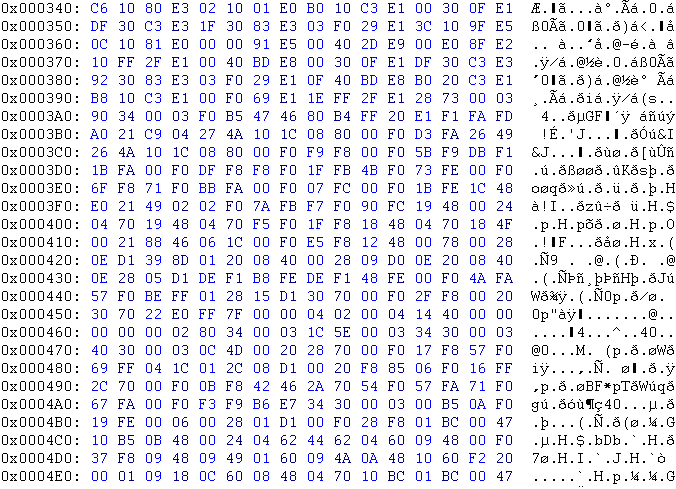
\includegraphics[width=12cm]{bases/img/hex.png}\\
        \caption*{Un éditeur hexadécimal montre le contenu d'un fichier, d'un disque dur, ou de la RAM d'un ordinateur. La première colonne indique l'adresse,
            puis 16 octets écrits en hexadécimal et enfin les caractères correspondants.}
    \end{center}
\end{figure}
\section{Hexadécimal et binaire : un mariage heureux}
Le grand avantage qu'apporte l'hexadécimal s'illustre facilement :

\begin{methode}[ 6 : passer de la base 2 à la base 16]
    \begin{tabbing}
        $(101101000011101)_2$	\=	$=(0101\ 1010\ 0001\ 1101)_2$\\
        \>	$=\left(\underbrace{0101}_5\ \underbrace{1010}_A\ \underbrace{0001}_1\ \underbrace{1101}_D\right)_2$\\
        \>	$=(5A1D)_{16}$
    \end{tabbing}
\end{methode}

\begin{methode}[ 7 : passer de la base 16 à la base 2]
    $(F7B)_{16}=\left(\underbrace{1111}_F\ \underbrace{0111}_7\ \underbrace{1011}_B\right)_2$
\end{methode}
\begin{figure}
    \begin{center}
        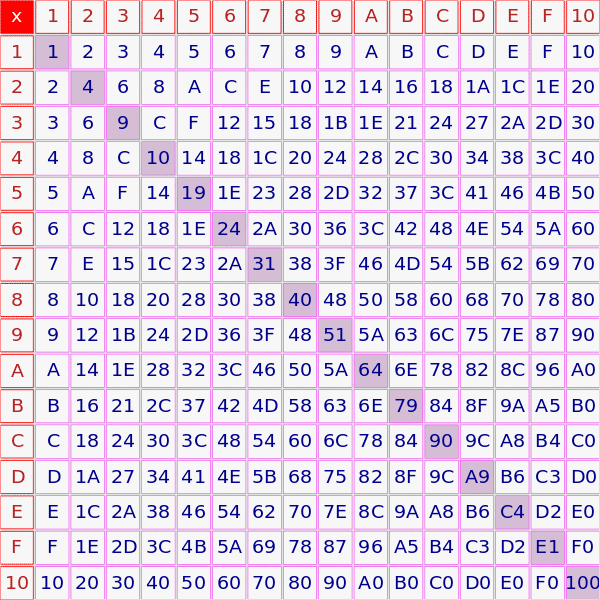
\includegraphics[width=10cm]{bases/img/hexmult.png}\\
        \caption*{Table de multiplication hexadécimale.}
    \end{center}
\end{figure}


\section{Additions}

On pose l'opération à la main : c'est la même chose qu'en base 10.
\subsection*{En base 2}
La seule différence avec la base 10 c'est que deux 1 donnent $(2)_{10}$ donc $(10)_2$, donc un zéro et une retenue de 1.
Quand il y a deux 1 et une retenue de 1 en plus, cela donne $(3)_{10}$ donc $(11)_2$, donc un 1 et une retenue de 1.

\tabulardefault
\begin{exemple}[]
    \begin{center}
        \begin{tabular}{ccccccccc}
              &   &   & $_1$ & $_1$ & $_1$ &   &   &   \\
              & 1 & 1 & 0    & 1    & 0    & 1 & 0 & 1 \\
            + &   &   &      & 1    & 1    & 1 & 0 & 0 \\
            \hline
            = & 1 & 1 & 1    & 1    & 0    & 0 & 0 & 1 \\
        \end{tabular} \\[2em]
    \end{center}
\end{exemple}

\subsection*{En base 16}

C'est encore la même chose. Il faut bien se souvenir de la valeur de A, B, C, D, E et F.\\
Ajouter 8 et 3 ne provoque pas de retenue puisque $8+3=11$ et que $11$ est $B$ en base 16.\\
Dès que l'addition de 2 chiffres dépasse 15, il y aura une retenue : par exemple 9 et A donnent $(19)_{10}$, donc $(13)_{16}$. Ainsi on note 3 et une retenue de 1.

\begin{exemple}
    \begin{center}
        \begin{tabular}{ccccc}
              &   & $_1$ &   &   \\
              & 2 & 4    & 9 & 8 \\
            + & 1 & 7    & A & 3 \\
            \hline
            = & 3 & C    & 3 & B \\
        \end{tabular}
    \end{center}
\end{exemple}

\section{Multiplications par 2 en binaire}

\begin{propriete}[]
    \begin{itemize}
        \item 	Multiplier un nombre écrit en binaire par 2 revient à décaler la virgule d'un cran vers la droite (ou ajouter un zéro à droite si le nombre est entier).
        \item 	Diviser un nombre écrit en binaire par 2 revient à décaler la virgule d'un cran vers la gauche.
    \end{itemize}
\end{propriete}

\begin{exemple}[s]
    \begin{itemize}
        \item 	$(1\ 0101)_2\times (2)_{10}=(10\ 1010)_2$
        \item 	$(11,01)_2\times (16)_{10}=(11\ 0100)_2$
        \item 	$(1\ 1101)_2\div (2)_{10}=(1110,1)_2$
        \item 	$(101)_2\div (32)_{10}=(0,0010\ 1)_2$
    \end{itemize}
\end{exemple}

\begin{remarque}
    Rappelons-nous que $(2)_{10}=(10)_2$, et que plus généralement $2^n$ s'écrit en binaire comme «  un 1 suivi de $n$ zéros » .
\end{remarque}



\section{Exercices}

\begin{exercice}
    \begin{enumerate}
        \item 	Calculer $2^6+2^4+2^3+2^0$.
        \item 	En déduire l'écriture binaire de 89.
    \end{enumerate}
\end{exercice}

\begin{exercice}
    \begin{enumerate}
        \item 	Calculer $2^7+2^3+2^2+2^1$.
        \item 	En déduire l'écriture décimale de  $(1000 1110)_2$.
    \end{enumerate}
\end{exercice}

\begin{exercice}[]
    En utilisant la méthode 2, donner l'écriture binaire de
    \begin{enumerate}
        \item 	56
        \item 	35
        \item 	13
    \end{enumerate}
\end{exercice}

\begin{exercice}[]
    En utilisant la méthode 3, donner l'écriture binaire de
    \begin{enumerate}
        \item 	142
        \item 	273
        \item 	1000
    \end{enumerate}
\end{exercice}

\begin{exercice}
    \begin{itemize}
        \item 	Donner l'écriture décimale de $(1101\ 1010)_2$.
        \item 	Donner l'écriture binaire de 2016.
        \item 	Donner l'écriture hexadécimale de 2016.
    \end{itemize}
\end{exercice}

\begin{exercice}
    \begin{itemize}
        \item 	Donner les écritures décimales de $(11)_2$, $(111)_2$, $(1111)_2$.
        \item   Soit $n \in \N$, conjecturer la valeur de $ \left(\underbrace{1\ldots 1}_{n\textrm{ chiffres}}\right)_2$.
    \end{itemize}
\end{exercice}

\begin{exercice}
    Pour multiplier par dix un entier naturel exprimé en base dix, il suffit d'ajouter un 0 à sa
    droite, par exemple, $12\times 10 = 120$.\\
    Quelle est l'opération équivalente pour les entiers naturels exprimés en base deux?
\end{exercice}

\begin{exercice}
    \begin{enumerate}
        \item 	Donner l'écriture binaire de 174.
        \item 	Donner celle de 17.
        \item 	Poser l'addition de 174 et 17 en binaire.
        \item 	Donner l'écriture décimale du résultat et vérifier.
    \end{enumerate}
\end{exercice}

\begin{exercice}
    \begin{enumerate}
        \item 	Donner l'écriture hexadécimale de 1022.
        \item 	Donner celle de 3489.
        \item 	Poser l'addition de 1022 et 3489 en hexadécimal.
        \item 	Donner l'écriture décimale du résultat et vérifier.
    \end{enumerate}
\end{exercice}

\begin{exercice}[]
    Ajouter $(1101\ 1011)_2$ et $(0011\ 0110)_2$ en posant l'opération.
\end{exercice}

\begin{exercice}[]
    On pose  $a=(1001)_2$, $b=(0010\ 1000)_2$ et $c=(0001\ 0111)_2$.\\
    
    Calculer $a +b+c$ en posant les opérations (on peut faire des étapes ou bien tout calculer en une fois).
\end{exercice}

\begin{exercice}[]
    On reprend les données de l'exercice précédent.	Calculer $a\times 4+b\div 8 +c$.
\end{exercice}

\begin{exercice}[]
    Calculer à la main $(AF3)_{16}+(8AD)_{16}$.
\end{exercice}

\begin{exercice}[]
    Calculer à la main $(123)_{16}+(456)_{16}+(789)_{16}$ en posant une seule opérations si possible.
\end{exercice}

\begin{exercice}[*]
    Le Roi d'un pays imaginaire fait frapper sa monnaie par 8 nains : chacun d'entre eux produit des pièces d'or de 10g chacune.\\
    
    Un jour, son Mage lui annonce : « Majesté, mon miroir magique m'a prévenu que certains de vos nains vous volent. Ils prélèvent 1g d'or sur chaque pièce qu'ils frappent. Pour vous aider à trouver les voleurs, voici une balance magique. Elle est précise au gramme près et peut peser autant que vous voulez. Malheureusement elle ne peut être utilisée qu'une fois.»\\
    
    Le lendemain, le Roi convoque les 8 nains en demandant à chacun d'apporter un coffre rempli de pièces d'or qu'il a frappées.\\
    On suppose que
    \begin{itemize}
        \item chaque nain dispose d'autant de pièces que nécessaire ;
        \item un nain honnête n'a que des pièces de 10g ;
        \item un nain voleur n'a que des pièces de 9g ;
    \end{itemize}
    Peux-tu aider le Roi pour démasquer les voleurs?
\end{exercice}
\newcommand{\carre}[2]
{\draw[thick,fill  = UGLiOrange!50] (#1+.1,#2+.1) rectangle (#1+.9,#2.9);
}





\begin{exercice}

    On dispose d'une clé de cryptage notée $\left(a_1,\:a_2,\:a_3,\:a_4,\:a_5\right) = (63, 62, 65, 68, 34)$.\\
    Cette clé, publiée par la personne destinataire, permet à quiconque de lui envoyer un message crypté. Voici comment on crypte le message.\\
    On associe d'abord à chaque lettre son rang dans l'alphabet, selon la correspondance suivante :
    \begin{center}
        \tabstyled
        \begin{tabularx}{\linewidth}{|l|*{13}{>{\centering \arraybackslash}X|}}\hline
            \ccell Lettre & A  & B  & C  & D  & E  & F  & G  & H  & I  & J  & K  & L  & M  \\ \hline
            \ccell Rang  & 1  & 2  & 3  & 4  & 5  & 6  & 7  & 8  & 9  & 10 & 11 & 12 & 13 \\ \hline
            \ccell Lettre & N  & O  & P  & Q  & R  & S  & T  & U  & V  & W  & X  & Y  & Z  \\ \hline
            \ccell Rang  & 14 & 15 & 16 & 17 & 18 & 19 & 20 & 21 & 22 & 23 & 24 & 25 & 26 \\ \hline
        \end{tabularx}
    \end{center}
    Pour crypter une lettre:
    \begin{itemize}
        \item on détermine son rang à l'aide du tableau de correspondance précédent ;
        \item on écrit ce nombre en base 2 sur 5 bits; on ainsi obtient 5 chiffres $\left(m_1, m_2, m_3,  m_4, m_5\right)$, chaque chiffre étant égal à $0$ ou à $1$ ;
        \item on détermine alors la valeur cryptée, égale à la somme $\sigma =  a_1m_1 + a_2m_2 + a_3m_3 + a_4m_4 + a_5m_5$.
    \end{itemize}
    On remarque qu'une lettre est ainsi cryptée par un nombre entier.\\
    \emph{Exemple} : on veut crypter la lettre «  I  ».
    
    \begin{itemize}
        \item Le rang de I est $9$  ;
        \item on écrit ce nombre en base deux sur 5 bits : $9_{10} = 8 + 1= (01001)_2$,
        \item on calcule la somme $\sigma=0 \times 63 + 1 \times62 + 0 \times 65 + 0 \times 68 + 1 \times 34 = 96$.
    \end{itemize}
    La lettre «  I  » est donc cryptée par l'entier $96$.\\
    
    \textbf{Question :} crypter la lettre «  W   » selon cette méthode.
\end{exercice}

\begin{exercice}[ : un petit jeu]
    On veut programmer un petit jeu : une bille commence dans la grille suivante, toujours à la case départ.\\
    On doit l'amener à la case arrivée en appuyant seulement sur les touches {$\rightarrow$}\ \ et {$\downarrow$}\ \ du clavier.
    Voici un exemple de partie :
    \begin{center}
        \begin{tikzpicture}
            \foreach \i in {0,1,2,3}
                {\foreach \j in {0,1,2,3}
                        {\carre{\i}{\j}}}
            \draw[thick,fill=UGLiBlue] (-.3,3.9)--(-.3,-.3)--(3.9,-.3)--(3.9,-.1)--(-.1,-.1)--(-.1,3.9)--cycle;
            \draw[thick,fill=UGLiBlue] (.1,4.1)--(4.1,4.1)--(4.1,.1)--(4.3,.1)--(4.3,4.3)--(.1,4.3)--cycle;
            \node[left] at (-.1,4.1) {départ};
            \node[right] at (4.1,-.1) {arrivée};
            \draw[ultra thick,->](0,4)--(0,3)--(2,3)--(2,2)--(3,2)--(3,0)--(4.1,0);
        \end{tikzpicture}
    \end{center}
    Pour représenter les différents parcours, on associe à chacun d'entre eux un entier de la manière suivante :
    \begin{itemize}
        \item 	on note la séquence de touches pressées dans l'ordre;
        \item 	on remplace chaque {$\downarrow$}\ \ par 0 et chaque {$\rightarrow$}\ \ par 1;
        \item 	on obtient l'écriture binaire de l'entier final.
    \end{itemize}
    \begin{enumerate}
        \item 	Justifier que l'entier obtenu à partir de l'exemple vaut 105.
        \item 	Combien faut-il de bits pour représenter un chemin donné ?
        \item 	Représenter le parcours associé au nombre 85.
        \item 	On considère un entier $N$ représentant un chemin.
              \begin{enumalph}
                  \item 	Est-il possible d'avoir $N=31$ ?
                  \item 	Rappeler ce que vaut $ (\underbrace{1...1}_{\text{k bits}})_2$.
                  \item 	Quel est le plus petit entier $N$ qui représente un chemin ? Dessiner le chemin associé.
                  \item 	Quel est le plus grand ? Dessiner le chemin associé.\\
              \end{enumalph}
    \end{enumerate}
\end{exercice}

\begin{exercice}[ : additions en base 2]
    Les additions «  à la main » en base 2 s'effectuent de la même manière qu'en base 10, la seule différence c'est que deux 1 donnent $(2)_{10}$ donc $(10)_2$, donc un zéro et une retenue de 1.
    Quand il y a deux 1 et une retenue de 1 en plus, cela donne $(3)_{10}$ donc $(11)_2$, donc un 1 et une retenue de 1. Par exemple,
    on veut calculer $(1101\ 0101)_2+(1\ 1100)_2$, on pose l'opération en mettant les retenues en rouge.
    \begin{center}
        \tabdefault
        \begin{tabular}{ccccccccc}
              &   &   &   & {\color{red}\textbf{\footnotesize 1}} & {\color{red}\textbf{\footnotesize 1}} &   &   &   \\
              & 1 & 1 & 0 & 1                                     & 0                                     & 1 & 0 & 1 \\
            + &   &   &   & 1                                     & 1                                     & 1 & 0 & 0 \\
            \hline
            = & 1 & 1 & 1 & 1                                     & 0                                     & 0 & 0 & 1 \\
        \end{tabular} \\[2em]
    \end{center}
    Le résultat est donc $(1111\ 0001)_2$.
    \begin{enumerate}
        \item 	Donner les écritures décimales de  $(1101\ 0101)_2$, $(1\ 1100)_2$, $(1111\ 0001)_2$ et vérifier qu'il n'y a pas d'erreur d'addition.
        \item 	Vérifier que l'on a bien l'égalité $138+111=249$ lorsque l'on effectue l'addition en binaire.
        \item 	Calculer $(1011\ 1101)_2+(11)_2$ et donner les écritures décimales des 3 nombres intervenant dans cette addition.\\
    \end{enumerate}
\end{exercice}

\begin{exercice}[ : entiers non signés sur un octet]
    Dans certains langages, on utilise un octet (c'est-à-dire 8 bits) pour stocker un entier positif. On stocke dans l'octet l'écriture binaire de l'entier, telle quelle.
    \begin{itemize}
        \item 	en C et C++, ce type de variable s'appelle \texttt{unsigned char};
        \item 	en C\#, il s'appelle \texttt{byte}.
    \end{itemize}
    \begin{enumerate}
        \item 	Quels sont les entiers représentables de cette manière ?
        \item 	Pour ajouter deux valeurs de ce type, on effectue l'addition en binaire, mais s'il y a une retenue à reporter à la fin (qui irait théoriquement dans un 9ème bit) on ne la prend pas en compte : on ne garde que les 8 premiers bits du résultats en partant de la droite.
              \begin{enumalph}
                  \item 	Ajouter avec cette méthode 129 et 130 et donner le résultat sous forme décimale.
                  \item	Ci dessus on a écrit un petit programme en C++. Dire ce qu'il fait et interpréter le résultat affiché dans la console.
              \end{enumalph}
              
              \begin{minted}[breaklines]{cpp}
                #include <iostream> // bibliothèque d'affichage
                int main() // début de la fonction principale
                {
                    unsigned char c = 0; // on définit la variable c
                    for (int i = 0; i < 300; i++) // on fait une boucle pour
                    {
                        std::cout << "valeur de i : " << i; // on affiche la valeur de i
                        std::cout << "  et valeur de c : " << (int)c; // on affiche la valeur de c en base 10
                        std::cout << endl; // on revient à la ligne (END Line)
                        c++; // on augmente c de 1
                    }
                    return 0; // la fonction principale renvoie zéro par convention
                }
            \end{minted}
              Voilà ce que la console affiche :\\
              
              \texttt{valeur de i : 0  et valeur de c : 0}\\
              \texttt{valeur de i : 1  et valeur de c : 1}\\
              \textit{et c\ae tera}\\
              \texttt{valeur de i : 254  et valeur de c : 254}\\
              \texttt{valeur de i : 255  et valeur de c : 255}\\
              \texttt{valeur de i : 256  et valeur de c : 0}\\
              \texttt{valeur de i : 257  et valeur de c : 1}\\
              \textit{et c\ae tera}\\
              \texttt{valeur de i : 298  et valeur de c : 42}\\
              \texttt{valeur de i : 299  et valeur de c : 43}\\
    \end{enumerate}
\end{exercice}

\begin{exercice}[ : entiers signés en complément à 2 sur 8 bits]
    Pour représenter un entier signé (positif ou négatif) sur un octet, on peut penser au système suivant : le bit de poids fort vaut 0 si l'entier est positif et 1 s'il est négatif. Les 7 autres bits servent à représenter la partie numérique du nombre.\\
    Par exemple, $$\Large(\color{UGLiRed}1\color{UGLiBlue}001\ 1010\color{black})_2$$
    représente un nombre négatif car son bit de poids fort est à 1. Sa partie numérique est $(1\ 1010)_2=26$, donc il représente -26.
    \begin{enumerate}
        \item 	\begin{enumalph}
                  \item 	Que représente $(0000\ 0000)_2$ ? Et $(1000\ 0000)_2$ ?
                  \item 	Donner la représentation de +26 et ajouter les représentations de +26 et -26 en binaire. Quel nombre représente le résultat obtenu ? Est-ce cohérent ?
              \end{enumalph}
        \item 	Pour pallier ces problèmes, on représente les entiers \textit{en complément à 2 sur 8 bits} :
              \begin{itemize}
                  \item si on veut représenter un entier compris entre 0 et $2^7-1=127$, alors on le représente tel quel sur un octet ;
                  \item si on veut représenter un entier $n$ compris entre $-2^8=-128$ et -1, alors on le représente par $n+256$.
              \end{itemize}
              \begin{center}
                  \begin{tikzpicture}[scale=.5]
                      \def\RayonListe{6.5}
                      \def\EpaisseurListe{1.5}
                      \def\LongueurListe{16}
                      \draw[fill = UGLiOrange!15] (0,0) circle(\RayonListe+\EpaisseurListe);
                      \draw[fill = white] (0,0) circle(\RayonListe);
                      \foreach \compt in {0,1,...,\numexpr\LongueurListe-1}
                          {\draw (90-\compt/\LongueurListe*360:\RayonListe)--(90-\compt/\LongueurListe*360:\RayonListe+\EpaisseurListe);}
                      \foreach \compt in {0,1,2}	{\draw (90-\compt/\LongueurListe*360-180/\LongueurListe:\RayonListe+\EpaisseurListe/2)node{\color{UGLiGreen}\compt};}
                      \foreach \compt in {3,4,5}	{\draw (90-\compt/\LongueurListe*360-180/\LongueurListe:\RayonListe+\EpaisseurListe/2)node{\color{UGLiGreen}...};}
                      \def \compt{6}	{\draw (90-\compt/\LongueurListe*360-180/\LongueurListe:\RayonListe+\EpaisseurListe/2)node{\color{UGLiGreen} 126};}
                      \def \compt{7}	{\draw (90-\compt/\LongueurListe*360-180/\LongueurListe:\RayonListe+\EpaisseurListe/2)node{ \color{UGLiGreen} 127};}
                      \def \compt{8}	{\draw (90-\compt/\LongueurListe*360-180/\LongueurListe:\RayonListe+\EpaisseurListe/2)node{\color{UGLiRed} -128};}
                      \def \compt{9}	{\draw (90-\compt/\LongueurListe*360-180/\LongueurListe:\RayonListe+\EpaisseurListe/2)node{ \color{UGLiRed} -127};}
                      \foreach \compt in {10,11,12}	{\draw (90-\compt/\LongueurListe*360-180/\LongueurListe:\RayonListe+\EpaisseurListe/2)node{\color{UGLiRed}...};}
                      \def \compt{13}	{\draw (90-\compt/\LongueurListe*360-180/\LongueurListe:\RayonListe+\EpaisseurListe/2)node{\color{UGLiRed} -3};}
                      \def \compt{14}	{\draw (90-\compt/\LongueurListe*360-180/\LongueurListe:\RayonListe+\EpaisseurListe/2)node{\color{UGLiRed} -2};}
                      \def \compt{15}	{\draw (90-\compt/\LongueurListe*360-180/\LongueurListe:\RayonListe+\EpaisseurListe/2)node{\color{UGLiRed} -1};}
                      \def\RayonListe{5}
                      \def\EpaisseurListe{1.5}
                      \def\LongueurListe{16}
                      \draw[fill=UGLiBlue!15] (0,0) circle(\RayonListe+\EpaisseurListe);
                      \draw[fill=white] (0,0) circle(\RayonListe);
                      \foreach \compt in {0,1,...,\numexpr\LongueurListe-1}
                          {\draw (90-\compt/\LongueurListe*360:\RayonListe)--(90-\compt/\LongueurListe*360:\RayonListe+\EpaisseurListe);}
                      \foreach \compt in {0,1,2}	{\draw (90-\compt/\LongueurListe*360-180/\LongueurListe:\RayonListe+\EpaisseurListe/2)node{\color{blue}\compt};}
                      \foreach \compt in {3,4,5}	{\draw (90-\compt/\LongueurListe*360-180/\LongueurListe:\RayonListe+\EpaisseurListe/2)node{\color{blue}...};}
                      \def \compt{6}	{\draw (90-\compt/\LongueurListe*360-180/\LongueurListe:\RayonListe+\EpaisseurListe/2)node{\color{blue} 126};}
                      \def \compt{7}	{\draw (90-\compt/\LongueurListe*360-180/\LongueurListe:\RayonListe+\EpaisseurListe/2)node{\color{blue}  127};}
                      \def \compt{8}	{\draw (90-\compt/\LongueurListe*360-180/\LongueurListe:\RayonListe+\EpaisseurListe/2)node{\color{blue}128};}
                      \def \compt{9}	{\draw (90-\compt/\LongueurListe*360-180/\LongueurListe:\RayonListe+\EpaisseurListe/2)node{\color{blue} 129};}
                      \foreach \compt in {10,11,12}	{\draw (90-\compt/\LongueurListe*360-180/\LongueurListe:\RayonListe+\EpaisseurListe/2)node{\color{blue}...};}
                      \def \compt{13}	{\draw (90-\compt/\LongueurListe*360-180/\LongueurListe:\RayonListe+\EpaisseurListe/2)node{\color{blue} 253};}
                      \def \compt{14}	{\draw (90-\compt/\LongueurListe*360-180/\LongueurListe:\RayonListe+\EpaisseurListe/2)node{\color{blue} 254};}
                      \def \compt{15}	{\draw (90-\compt/\LongueurListe*360-180/\LongueurListe:\RayonListe+\EpaisseurListe/2)node{\color{blue} 255};}
                  \end{tikzpicture}
              \end{center}
              Ce schéma représente l'encodage des entiers relatifs en complément à 2 sur 8 bits (que l'on retrouve dans le type \texttt{char} en C et C++).\\
              
              En bleu figurent les nombres tels qu'ils sont stockés dans la mémoire, sur un octet.\\
              En orange figurent les nombres représentés par les nombres bleus :
              \begin{itemize}
                  \item 	lorsqu'il est compris entre 0 et 127, un nombre bleu représente ce même nombre (affiché en vert);
                  \item 	lorsqu'il est compris entre 128 et 255, un nombre bleu $p$ représente le nombre $p-256$ (affiché en rouge).
              \end{itemize}
              \begin{enumalph}
                  \item 	Donner la représentation en complément à 2 sur 8 bits du nombre +7.
                  \item 	Faire de même avec -3.
                  \item 	Ajouter en binaire ces deux représentations (une éventuelle retenue après le 8\eme bit est ignorée), quel nombre cela représente-t-il ?
              \end{enumalph}
        \item  Recommencer la question précédente et vérifier que l'égalité $-12+8=-4$ est vérifiée en complément à 2 sur 8 bits.\\
        \item Le programme suivant affiche -116. Expliquer ce résultat.
              \begin{minted}{cpp}
                #include <iostream> // nécessaire pour utiliser cout
                int main() // début de la fonction main
                {
                    char c1 = 120; // on définit une première variable
                    char c2 = 20; // puis une deuxième
                    char c3 = c1+c2; // on les ajoute
                    std::cout << (int) c3; // on affiche le résultat en base 10
                    return 0; // la fonction main renvoie traditionnellement zéro
                }
            \end{minted}
    \end{enumerate}
\end{exercice}




\begin{exercice}[ : masque jetable]
    Le but de cet exercice est d'étudier une méthode de cryptage inventée par Gilbert Vernam en 1917, et appelée «  masque jetable  ».
    Dans tout l'exercice, on note respectivement $M$ le mot initial, $K$ la clé de cryptage et $Y$ le mot crypté.
    Les trois nombres $M$, $K$, $Y$ sont des entiers naturels.
    Les chiffres hexadécimaux sont notés 0, 1, 2, 3, 4, 5, 6, 7, 8, 9, A, B, C, D, E, F.
    
    \begin{enumerate}
        \item Questions préliminaires :
              \begin{enumalph}
                  \item Donner la représentation en hexadécimal de l'entier binaire $1011101_2$.
                  \item Calculer en travaillant dans le système hexadécimal les sommes $(7)_{16} + (4)_{16}$ et $(A)_{16} + (C)_{16}$.
              \end{enumalph}
        \item Soit $M$ et $K$ deux entiers naturels écrits en hexadécimal, tels que la longueur de l'écriture de $K$ est supérieure ou égale à celle de $M$, et tels que l'écriture de $K$ ne comporte aucun chiffre $0$.
              
              Pour crypter le mot $M$ avec la clé $K$, on procède comme suit : pour chaque  chiffre $m$ du mot
              initial $M$, on considère le chiffre $k$ de la clé $K$ qui a la même position que $m$ dans l'écriture.
              
              On obtient alors le chiffre $y$ du mot crypté $Y$ qui a la même position que $m$ dans l'écriture du mot initial $M$, de la façon suivante : $y$ est le chiffre hexadécimal des unités de la somme $m + k$.
              
              Le mot crypté $Y$ est déterminé en hexadécimal par la juxtaposition dans le même ordre des
              chiffres $y$ calculés pour chaque chiffre $m$ du mot $M$.
              \begin{center}
                  \begin{tabularx}{\linewidth}{|X|}\hline
                      \emph{Exemple} : avec $M =(49)_{16}$ et $K = (19)_{16}$
                      \begin{itemize}
                          \item Avec le chiffre de rang 1 en partant de la droite : $m = 9$ et $k = 9$ ; donc $m + k = (12)_{16}$ et par suite $y = 2$ ;
                          \item avec le chiffre de rang 2 : $m = 4$ et $k = 1$ ; donc $m +k = (5)_{16}$ et par suite $y = 5$.
                      \end{itemize} \\\hline
                  \end{tabularx}
              \end{center}
              
              Donc le mot crypté est $Y = (52)_{16}$.
              
              \smallskip
              
              \textbf{Question }: avec le mot initial $M = (7 A)_{16}$ et la clé $K = (4C)_{16}$, déterminer le mot crypté $Y$.
        \item Par cette méthode, on admet que le décryptage suit les mêmes étapes en remplaçant la clé $K$ par une autre clé $K'$. Lorsque l'écriture de $K$ comporte au maximum deux chiffres hexadécimaux,
              la clé $K'$ est l'écriture en hexadécimal de la différence (écrite en décimal) $(272)_{10} - (K)_{10}$.
              
              \smallskip
              
              Cette question est une question à choix multiple. Une seule réponse est exacte. Recopier sur la
              copie seulement la réponse exacte. On ne demande pas de justification.
              
              \smallskip
              
              Avec la clé de cryptage $K = (19)_{16}$, la clé de décryptage $K'$ est égale à :
              
              \begin{center}
                  \begin{tabularx}{0.75\linewidth}{X X}
                      \textbf{Réponse A~~} : $(253)_{16}$ & \textbf{Réponse B~~} : $(247)_{16}$ \\
                      \textbf{Réponse C~~} : $(FD)_{16}$  & \textbf{Réponse D~~} : $(F7)_{16}$  \\
                  \end{tabularx}
              \end{center}
    \end{enumerate}
\end{exercice}



\chapter{\'Ecriture des « réels » }
\introduction{Tout cela est-il bien réel ?}

\section{\'Ecriture décimale et arrondi}
On sait que tout nombre réel admet une écriture décimale :
\begin{itemize}
	\item 	« un et demi  »  s'écrit $\np{1,500000}$\ldots\ et on enlève les zéros inutiles, cela fait $1,5$.
	\item 	«trois septièmes  »  s'écrit $\np{0,4285714285714285714285714}\ldots$ et pour insister sur le fait que le motif 428571
	      se répète indéfiniment on écrit $0,\underline{\np{428571}}$.
	\item 	$\pi$ a une écriture décimale qui commence par $\np{3,14159265359}$ mais son écriture décimale comporte une infinité de chiffres
	      \textit{sans qu'aucun motif ne se répète}.
\end{itemize}
On est souvent amenés à \textit{arrondir} les nombres réels : soit le nombre n'est «pas très grand »  et on ne veut garder que quelques chiffres
après la virgule, soit il est «plutôt grand »  et on ne veut garder que quelques chiffres significatifs :

\begin{methode}[ 1]
	On veut arrondir $\frac{3}{7}$ à $10^{-3}$ près, c'est-à-dire à 3 chiffres après la virgule.\\
	Il y a trois possibilités :
	\begin{itemize}
		\item 	\textbf{Arrondi par défaut} : On «coupe »  après le troisième chiffre :\\
		      $$\frac{3}{7}\approx 0,428\quad\textrm{à }10^{-3}\textrm{ près par défaut.}$$
		\item 	\textbf{Arrondi par excès} : On «coupe »  après le troisième chiffre et on ajoute $10^{-3}$,
		      c'est-à-dire un \textit{millième} :\\
		      $$\frac{3}{7}\approx 0,429\quad\textrm{à }10^{-3}\textrm{ près par excès.}$$
		\item 	\textbf{Arrondi au plus près} : On regarde le chiffre immédiatement après le troisième (celui qui correspond
		      à $10^{-4}$). Si c'est 0,1,2,3 ou 4, on prend l'arrondi par défaut, si c'est 5,6,7,8 ou 9, on prend l'arrondi
		      par excès.
		      $$\frac{3}{7}\approx 0,429\quad\textrm{à }10^{-3}\textrm{ au plus proche.}$$
	\end{itemize}
\end{methode}

\begin{exercice}[]
	Utiliser la méthode 1 pour déterminer
	\begin{enumerate}
		\item 	L'arrondi de $\frac{13}{11}$ à $10^{-2}$ près par défaut
		\item 	L'arrondi de $\sqrt{2}$ à $10^{-4}$ près par excès.
		\item 	L'arrondi de $\frac{149}{999}$ à $10^{-3}$ au plus près.
	\end{enumerate}
\end{exercice}

\begin{methode}[ 2]
	On veut arrondir $\np{273692,291}$ à $10^{4}$, c'est à dire à la dizaine de milliers.\\
	Là encore il y a trois possibilités. On commence par remarquer que le chiffre correspondant à $10^4$ est le 7.
	\begin{itemize}
		\item 	\textbf{Arrondi par défaut} : On remplace tous les chiffres à droite du 7 par des zéros. La partie décimale disparaît.
		      $$ \np{273692,291}\approx \np{270000}\quad\textrm{à }10^{4}\textrm{ près par défaut.}$$
		\item  	\textbf{Arrondi par défaut} : On prend l'arrondi par défaut et on ajoute $10^4$.
		      $$ \np{273692,291}\approx \np{280000}\quad\textrm{à }10^{4}\textrm{ près par excès.}$$
		\item 	\textbf{Arrondi au plus près} : On regarde le chiffre immédiatement après celui de $10^4$ (celui qui correspond
		      à $10^{3}$). Si c'est 0,1,2,3 ou 4, on prend l'arrondi par défaut, si c'est 5,6,7,8 ou 9, on prend l'arrondi
		      par excès.
		      $$ \np{273692,291}\approx \np{270000}\quad\textrm{à }10^{4}\textrm{ au plus proche.}$$
	\end{itemize}
\end{methode}

\begin{exercice}[]
	Utiliser la méthode 2 pour déterminer
	\begin{enumerate}
		\item 	L'arrondi de $\np{38564526}$ à $10^3$ près par défaut
		\item 	L'arrondi de $\np{281 564 526}$ à $10^8$ près par excès.
		\item 	L'arrondi de $\np{9524}$ à $10^{3}$ au plus près.
	\end{enumerate}
\end{exercice}

\section{\'Ecriture dyadique et arrondi}

\subsection{\'Ecriture dyadique}
Lorsqu'on écrit un nombre décimal tel que $\np{3,719}$, on a l'égalité suivante:
$$\np{3,719}=3\times 10^0+7\times 10^{-1}+1\times 10^{-2}+9\times 10^{-3}$$
Il est possible de faire la même chose en base 2 : on ajoute des puissances de 2 d'exposants négatifs.

\begin{methode}[ : retrouver l'écriture décimale à partir d'une écriture dyadique]
	On considère le nombre $n=(1010,011)_2$. Quelle est son écriture décimale ?
	\begin{itemize}
		\item 	Sa partie entière est $(1010)_2$, ce qui vaut 10.
		\item 	Sa partie décimale est
		      \begin{tabbing}
			      $(0,011)_2$ \= $=2^{-2}+2^{-3}$\\
			      \>  $=0,25+0,125$\\
			      \>	$=0,375$
		      \end{tabbing}
	\end{itemize}
	Ainsi $$n=10,375$$
\end{methode}
\begin{exercice}[]
	Utiliser la méthode précédente pour déterminer les écriture décimales de
	\begin{enumerate}
		\item 	$(0,101)_2$
		\item 	$(11,01)_2$
		\item 	$(1111,1111)_2$
	\end{enumerate}
\end{exercice}

\begin{methode}[ : construire un nombre dyadique]
	On veut l'écriture du nombre $5,75$ en base 2. Pour la partie entière, c'est simple : $$5=(101)_2$$
	Pour la partie décimale, on remarque que
	\begin{tabbing}
		$0,75$ \= $=0,5+0,25$\\
		\> 	$=\frac{1}{2}$ +$\frac{1}{4}$\\
		\>	$=2^{-1}+2^{-2}$\\
	\end{tabbing}
	Ainsi $$0,75 = (0,11)_2$$
	Finalement $$5,75=(101,11)_2$$
\end{methode}

\begin{exercice}[]
	Utiliser la méthode précédente pour déterminer les écriture dyadiques de
	\begin{enumerate}
		\item 	$3,25$
		\item 	$12,625$
		\item 	$7,8125$
	\end{enumerate}
\end{exercice}

\begin{remarque}[]
	Un nombre décimal n'a pas généralement une écriture dyadique «qui se termine » .\\
	Par exemple 0,1 (qui est pourtant le nombre décimal le plus simple auquel on puisse penser) s'écrit
	$$0,1 = (0,\ 0001\ 1001\ 1001\ \underline{1001} ...)_2$$
\end{remarque}

\subsection{Arrondi}

Pour arrondir un nombre en base 2, on fait pareil qu'en base 10 :

\begin{exemple}[s]
	\begin{enumerate}
		\item 	Arrondissons $n=(1101\ 1010)_2$ à $2^4$ au plus proche :\\
		      L'arrondi par défaut est $(1101\ 0000)_2$ mais comme le bit juste à droite du bit de $2^4$ est un 1, il faut rajouter $2^4$ à
		      notre valeur arrondie, pour avoir la valeur par excès qui, elle, est plus proche :
		      \begin{center}
			      \begin{tabular}{ccccccccc}
				        &   &   & $_1$ &   &   &   &   &   \\
				        & 1 & 1 & 0    & 1 & 0 & 0 & 0 & 0 \\
				      + & 0 & 0 & 0    & 1 & 0 & 0 & 0 & 0 \\
				      \hline
				      = & 1 & 1 & 1    & 0 & 0 & 0 & 0 & 0 \\
			      \end{tabular} \\[2em]

			      Ainsi $n\approx (1110\ 0000)_2$ à $2^4$ au plus proche.
		      \end{center}
		\item 	Pour les nombres dyadiques, c'est la même chose. Arrondissons $m=(11,\ 0011\ 1001)_2$ à $2^{-5}$ au plus proche :\\
		      Le bit de $2^{-6}$ est un 0, donc la bonne valeur arrondie est par défaut :
		      $$m\approx(11,\ 0011\ 1)_2\textrm{ à }2^{-5}\textrm{ au plus proche.}$$
	\end{enumerate}
\end{exemple}

\begin{remarque}
	Quand on nous demande d'arrondir sans préciser, on convient que c'est au plus proche.
\end{remarque}

\begin{exercice}[]
	Utiliser la méthode précédente pour déterminer
	\begin{enumerate}
		\item 	L'arrondi de $(1101\,1010)_2$ à $2^3$ près par défaut.
		\item 	L'arrondi de $(1,1110\,101)_2$ à $2^{-3}$ près par excès.
		\item 	L'arrondi de $(0,001)$ à $2^{-1}$ au plus proche.
	\end{enumerate}
\end{exercice}

\begin{exercice}[]
	Donner l'écriture décimale des nombres suivants\begin{enumerate}
		\item 	$(101,1)_2$
		\item 	$(1,011)_2$
		\item 	$(0,1111\ 111)_2$ en remarquant que c'est «$(111\ 1111)_2$ divisé par $2^7$.
	\end{enumerate}
\end{exercice}
\begin{exercice}[]
	\'Ecrire en base 2 les nombres suivants :
	\begin{enumerate}
		\item 	3,5
		\item 	7,75
		\item 	27,625
	\end{enumerate}
\end{exercice}

\begin{exercice}[]
	\begin{enumerate}
		\item 	Quel est l'arrondi de $(10,011)_2$ à $(0,1)_2$ près ?
		\item 	Quel est l'arrondi de $(1 1011)_2$ à $(100)_2$ près ?
		\item 	Quel est l'arrondi de $(0,0010 11)_2$ à $(0,0001)_2$ près ?
	\end{enumerate}
\end{exercice}

\begin{exercice}[]
	\begin{enumerate}
		\item 	Quel est l'arrondi de $(11,0101)_2$ à $2^{-2}$ près ?
		\item 	Quel est l'arrondi de $(1011 1011)_2$ à 32 près près ?
	\end{enumerate}
\end{exercice}

\begin{exercice}[**]
	On aimerait trouver l'écriture dyadique (illimitée) de $\dfrac{1}{3}$.
	On note donc $$\dfrac{1}{3}=(0,a_1a_2a_3\ldots)_2$$
	où $a_i$ vaut 1 ou 0.
	\begin{enumerate}
		\item 	Expliquer pourquoi $a_1$ vaut \textit{nécessairement 0}.
		\item 	On note $x=\frac{1}{3}$. Montrer que $x$ vérifie $4x=1+x$.
		\item 	Quelle est l'écriture dyadique de $4x$ ?
		\item 	Quelle est celle de $1+x$ ?
		\item 	En écrivant que ces 2 écritures représentent le même nombre, en déduire que $$\dfrac{1}{3}=(0,0101\ 0101\ldots )_2$$
	\end{enumerate}
\end{exercice}


\newcommand{\tabstrut}{\vrule height 1.25em depth 0.5em width 0pt}
\chapter{Arithmétique modulaire}

\section{Entiers naturels et division euclidienne}

\begin{definition}[ (rappel) : ensemble des entiers naturels]
	On note $\N$ l'ensemble des \textit{entiers naturels}. $$\N=\lbrace 0;\,1;\,2;\,3;\,4;\,5;\,6;\,7;\,8;\,9;\,10;\,11;\,12\ldots\rbrace$$
\end{definition}

\begin{definition}[ (rappel) : division euclidienne dans \N]
	
	Soient A et B deux entiers naturels, et $B\neq 0$. Il existe deux nombres uniques Q et R (vérifiant $0\leqslant R<B$) tels que l'on puisse écrire
	$$A = Q\times B + R$$
	
	C'est exactement la division que l'on a apprise en sixième (celle où l'on s'arrête aux nombres entiers):
	\begin{center}

		\begin{tabular}{r|l}
			A & B \\
			\cline{2-2}
			R & Q
		\end{tabular}
		
	\end{center}
	\begin{itemize}
		\item 	A est appelé le \textit{dividende};
		\item 	B est le \textit{diviseur};
		\item	Q est le \textit{quotient};
		\item 	R est le \textit{reste}, il est \textit{impérativement} plus petit que B.
	\end{itemize}
	
\end{definition}

\begin{exemple}[s]
	Effectuons la division euclidienne de 27 par 7 :
	\begin{center}
		\begin{tabular}{r|l}
			27 & 7 \\
			\cline{2-2}
			6  & 3
		\end{tabular}
	\end{center}
	Ainsi on a $\displaystyle\underbrace{27}_{A}=\underbrace{3}_{Q}\times \underbrace{7}_{B}+\underbrace{6}_{R}$.\\[3em]
	
	Effectuons la division euclidienne de 297 par 11 :
	\begin{center}
		\begin{tabular}{r|l}
			297 & 11 \\
			\cline{2-2}
			0   & 27
		\end{tabular}
	\end{center}
	Ainsi on a $\displaystyle\underbrace{286}_{A}=\underbrace{26}_{Q}\times \underbrace{11}_{B}+\underbrace{0}_{R}$.
\end{exemple}

\begin{exercice}[]
	Effectuer les divisions euclidiennes suivantes :
	\begin{multicols}{4}
		\begin{enumalph}
			\item 	28 par 8
			\item 	100 par 9
			\item 	379 par 11
			\item 	427 par 13\\
		\end{enumalph}
	\end{multicols}
\end{exercice}



\begin{definition}[ : diviseurs et multiples]
	Quand la division euclidienne de A par B donne un reste nul (lorsqu'elle tombe juste) on dit que \emph{B est un diviseur de A} ou bien (ce qui revient au même) que \emph{A est un multiple de B}.
\end{definition}

\begin{exemple}[s]
	\begin{itemize}
		\item 	$27 = 3\times 7 +4$ donc 7 ne divise pas 27 (7 n'est pas \textit{un diviseur} de 27).\\
		      On peut dire aussi que 27 n'est pas multiple de 7.
		\item 	$286 = 26\times 11+0$ donc 1 est donc un diviseur de 286.
	\end{itemize}
\end{exemple}
\begin{remarque}[s]
	\begin{enumalph}
		\item 	$28 = 4\times 5 +8$ mais ce n'est pas la division euclidienne de 28 par 5 car le  «  reste »  8 n'est pas plus petit que 5.
		\begin{tabbing}
			$28$ 	\= 	$=4\times 5 + 8$\\
			\>	$=4\times 5 + 5 + 3$\\
			\>	$=5\times 5 +3\qquad$ voilà la division euclidienne.
		\end{tabbing}
		\item 	\textit{ «  une division euclidienne n'en donne pas toujours 2 » 	} :\\
		$27 = 3\times 7 + 4$ est la division euclidienne de 27 par 7.\\
		On peut réarranger : $27 = 7\times 3 +4$ mais ce n'est pas la division euclidienne de 27 par 3  car le reste est trop grand.\\
		
		Ceci dit quand le reste est suffisamment petit, on obtient  «  2 divisions pour le prix d'une  » :
		$162=12\times 13 +1$ est la division euclidienne de 162 par 12, et de 162 par 13 aussi.
		
		\item 	\textit{ «  une division euclidienne qui tombe juste en donne deux en général » } :\\
		$297=27\times 11$ nous donne 2 diviseurs de 297 : 27 et 11.\\
		$16 = 4\times4$ aussi... mais c'est deux fois le même !
		\item 	avec la calculatrice, pour savoir si $B$ divise $A$ il suffit d'entrer $A\div B$ et de regarder si le résultat est entier.
	\end{enumalph}
\end{remarque}


\begin{exercice}[]
	Les égalités suivantes, peuvent-elles être des divisions euclidiennes ?\\
	Si oui, préciser A, B, Q et R.
	\begin{multicols}{2}
		\begin{enumalph}
			\item 	$65=32\times 2 +1$
			\item 	$80=5\times 10 + 30$
			\item 	$100 = 9\times 11 +1$
			\item 	$17=    3\times4 +5	$
		\end{enumalph}
	\end{multicols}
\end{exercice}

\begin{exercice}[]
	
	Les égalités suivantes ne sont pas des divisions euclidiennes.\\
	Transformez-les pour qu'elles le deviennent (il peut y avoir plusieurs possibilités).
	
	\begin{multicols}{2}
		\begin{enumalph}
			\item 	$19=3\times 4 + 7$
			\item 	$30=2\times 10 + 10$
			\item 	$29 = 4\times 5 +9$
			\item 	$23=  4\times 7 -5$\\
		\end{enumalph}
	\end{multicols}
\end{exercice}



\begin{pyc}
	\begin{minted}{python}
>>> a = 17   # déclare une variable a de type int (entier)
>>> b = 5    # idem avec b
>>> q = a // b # // donne le quotient par b

>>> q
5

>>> r = a % b  # %  donne le reste modulo b
>>> r
2	
\end{minted}
\end{pyc}

\section{Diviseurs et nombres premiers}

\begin{propriete}
	Soient $a$ et $b$ deux entiers naturels. Dire que $b$ est un diviseur de $a$ veut dire que la division euclidienne de $a$ par $b$ donne un reste nul.\\
	Cela signifie donc qu'il existe un entier naturel $k$ tel que $$a=k\times b$$
	On peut également dire que $a$ est multiple de $b$.
\end{propriete}

\begin{remarque}
	Si $b$ divise $a$ il existe un entier naturel $k$ tel que $$a=k\times b$$ et donc $k$ divise $a$ également.
\end{remarque}

\begin{exemple}[]
	$20=5\times 4$ donc 5 et 4 sont deux diviseurs de 20.
\end{exemple}

\begin{exercice}[]
	À l'aide de la calculatrice (ou non), déterminer si $b$ divise $a$.
	\begin{enumalph}
		\item 	$a=251$ et $b=13$
		\item 	$a=8$ et $b=80$
		\item 	$a=111$ et $b=37$
		\item 	$a=\np{131072}$ et $b=\np{8192}$\\
	\end{enumalph}
\end{exercice}


\begin{propriete}[s]
	\begin{itemize}
		\item 	Si a est divisible par b alors tout multiple de a est également divisible par b.
		\item 	Si a est divisible par b et que b est divisible par c alors a est divisible par c.
		\item 	Si a et b sont divisibles par c alors a+b aussi et (si a>b)  a-b aussi.
	\end{itemize}
\end{propriete}
\begin{exemple}[s]
	\begin{enumalph}
		\item 	12 est divisible par 3 donc tout multiple de 12 aussi : \np{12000} est donc divisible par 3.
		\item 	120 est divisible par 12 et 12 est divisible par 3 donc 120 est divisible par 3.
		\item 	Puisque \np{12000} et 12 sont divisibles par 3, \np{12000}-12, soit \np{11988}, l'est aussi.
	\end{enumalph}
\end{exemple}
\begin{definition}[ : entier naturel premier]
	Un entier naturel est dit \textit{premier} lorsqu'il admet 2 diviseurs \textit{distincts} : 1 et lui-même.
	\begin{itemize}
		\item 	0 n'est pas premier : $0=1\times 0=2\times 0=3\times 0=...$
		\item 	1 n'a qu'un diviseur : lui-même. Il n'est pas premier.
		\item 	2 est premier.
		\item 	3 aussi.
		\item 	4 ne l'est pas car 1, 2 et 4 divisent 1.
	\end{itemize}
\end{definition}

Il est assez simple de montrer qu'il y a une infinité de nombres premiers. Les nombres premiers jouent un rôle très important en mathématiques et interviennent dans les systèmes de cryptographie (basiques ou sophistiqués).

\begin{exercice}[ : crible d'\'Eratosthène]
	
	Dans la grille suivante :
	\begin{itemize}
		\item 	Entourer 2 et barrer 2 et tous ses multiples.
		\item 	Une fois cela fait, 3 est le premier nombre non barré après 2 donc on l'entoure et on barre tous ses multiples.
		\item 	Continuer jusqu'à ce que tous les nombres de la grilles soient traités (soit barrés soit entourés).
		\item 	Les nombres entourés sont \textit{des nombres premiers}.
	\end{itemize}
	\begin{center}
		\tabstyle[UGLiOrange]
		\xdef\x{0}
		\begin{tabular}{|*{10}{>{\tabstrut\xdef\x{\the\numexpr\x+1\relax}\ifnum\x=1\cellcolor{white} \else\x\fi}c|}}
			\hline
			 &  &  &  &  &  &  &  &  & \\
			\hline
			 &  &  &  &  &  &  &  &  & \\
			\hline
			 &  &  &  &  &  &  &  &  & \\
			\hline
			 &  &  &  &  &  &  &  &  & \\
			\hline
			 &  &  &  &  &  &  &  &  & \\
			\hline
			 &  &  &  &  &  &  &  &  & \\
			\hline
			 &  &  &  &  &  &  &  &  & \\
			\hline
			 &  &  &  &  &  &  &  &  & \\
			\hline
			 &  &  &  &  &  &  &  &  & \\
			\hline
			 &  &  &  &  &  &  &  &  & \\
			\hline
		\end{tabular}
	\end{center}
	
	Recopier ici la liste des nombres premiers trouvés :\\[3em]
	
\end{exercice}



\begin{propriete}[]
	Soit $n$ un entier supérieur ou égal à 2 :\begin{itemize}
		\item 	ou bien $n$ possède un diviseur inférieur ou égal à $\sqrt{n}$ et, à ce moment là, $n$ \textit{n'est pas premier.}
		\item 	ou bien \textit{aucun nombre premier } inférieur à $\sqrt{n}$ ne divise $n$ et \textit{il est premier}.
	\end{itemize}
\end{propriete}



\begin{methode}[ : déterminer si un nombre est premier ou non]
	Voici le début de la liste des nombres premiers :
	$$\lbrace 2;\ 3;\ 5;\ 7;\ 11;\ 13;\ 17;\ 19\rbrace$$
	\begin{itemize}
		\item 	133 est-il premier ?\\
		      
		      $\sqrt{133}\approx 11,5$ donc on regarde si 133 est divisible par 2, 3, 5, 7 ou 11.\\
		      On trouve que 133 = $19\times 7$ donc 133 n'est pas premier.
		\item 	251 est-il- premier ?\\
	
		      $\sqrt{251}\approx 15,8$ donc on regarde si 251 est divisible par 2, 3, 5, 7, 11, ou 13.\\
		      Ce n'est pas le cas : 251 est donc premier.
	\end{itemize}
\end{methode}

\begin{exercice}[]
	
	
	Les nombres suivants sont ils premiers ?
	
	\begin{multicols}{2}
		\begin{enumalph}
			\item 143
			\item 145
			\item 141
			\item 147
			\item 247
			\item 257
		\end{enumalph}
	\end{multicols}
	
\end{exercice}


\begin{propriete}[ : décomposition en produit de facteurs premiers]
	Tout entier naturel supérieur ou égal à 2 se décompose de manière unique (à l'ordre près) en \textit{produit de facteurs premiers}.
\end{propriete}

\begin{methode}[]
	Pour décomposer un nombre en produit de facteurs premiers, on cherche n'abord ses petits diviseurs premiers et on recommence jusqu'à trouver 1 :
	\begin{center}
		\tabdefault
		\begin{tabular}{r|l}
			234 & 2 \hspace*{3ex}on voit que 234 est pair                              \\
			117 & 3 \hspace*{3ex}car 3 est le plus petit nombre premier qui divise 117 \\
			39  & 3 \hspace*{3ex}et ainsi de suite                                     \\
			13  & 13\hspace*{3ex}...                                                   \\
			1   & \hspace*{4.55ex}on arrête
		\end{tabular}
	\end{center}
	On a donc
	\begin{tabbing}
		234 \= $=2\times 3\times 3\times 13$\\
		\> $=2\times 3^2\times 13\qquad$ et c'est la décomposition en produit de facteurs premiers de 234.
	\end{tabbing}
\end{methode}



\begin{exercice}[]
	
	Décomposer les nombres suivants en produit de facteurs premiers.
	
	\begin{multicols}{2}
		\begin{enumalph}
			\item 30
			\item 60
			\item 96
			\item 684
		\end{enumalph}
	\end{multicols}
\end{exercice}


\begin{methode}[ : liste des diviseurs d'un entier]
	Pour trouver \textit{tous} les divieurs d'un entier supérieur ou égal à 2 :
	\begin{enumalph}
		\item 	on le décompose en produit de facteurs premiers.
		\item 	on écrit tous les nombres que l'on peut former en prenant  «  moins de facteurs »  dans cette décomposition.
	\end{enumalph}
\end{methode}

\begin{exemple}[]
	Trouvons tous les diviseurs de 60 : \\
	$60=2\times30=2^2\times 15=2^2\times 3\times 5$.
	Ses diviseurs sont donc \\
	
	\begin{tabular}{l|l}
		1  & $2^0\times 3^0\times 5^0$ \\
		5  & $2^0\times 3^0\times 5^1$ \\
		3  & $2^0\times 3^1\times 5^0$ \\
		15 & $2^0\times 3^1\times 5^1$ \\
		2  & $2^1\times 3^0\times 5^0$ \\
		10 & $2^1\times 3^0\times 5^1$ \\
		6  & $2^1\times 3^1\times 5^0$ \\
		30 & $2^1\times 3^1\times 5^1$ \\
		4  & $2^2\times 3^0\times 5^0$ \\
		20 & $2^2\times 3^0\times 5^1$ \\
		12 & $2^2\times 3^1\times 5^0$ \\
		60 & $2^2\times 3^1\times 5^1$ \\
	\end{tabular}
\end{exemple}

Il est très facile d'oublier des diviseurs. Pour que cela n'arrive pas il faut utiliser une méthode logique pour les énumérer.\\
Voici un exemple d'algorithme qui les donne tous, en reprenant l'exemple de 60.

\begin{encadrecolore}{Algorithme}{UGLiBlue}
	\begin{verbatim}
Variables
i, j, k : entiers
Début
    Pour i allant de 0 à 2
        Pour j allant de 0 à 1
            Pour k allant de 0 à 1
                Afficher 2 ^ i * 3 ^ j * 5 ^ k
            FinPour
        FinPour
    FinPour
Fin
\end{verbatim}
\end{encadrecolore}

\begin{exercice}[]
	
	Donner la liste des diviseurs des nombres suivants.
	
	\begin{multicols}{2}
		\begin{enumalph}
			\item 30
			\item 25
			\item 96
			\item 684
		\end{enumalph}
	\end{multicols}
	
\end{exercice}


\section{pgcd de deux entiers naturels non nuls}

Deux entiers naturels non nuls ont au moins un diviseur commun : 1. Parmi tous les nombres qui les divisent tous les deux il y en a un plus grand : leur pgcd.

\begin{definition}[]
	Soient $a$ et $b$ deux entiers naturels non nuls.\\
	On note $pgcd(a;b)$ et on lit  «  pgcd de $a$ et de $b$ »  le plus grand entier qui divise à la fois $a$ et $b$.
\end{definition}

\begin{exemple}[s]
	Le plus grand nombre qui divise à la fois 12 et 16, c'est 4. Ainsi $pgcd(12;16)=4$.\\
	25 et 27 n'ont aucun diviseur commun plus grand que 1 : $pgcd(25;27)=1$.\\
\end{exemple}

\begin{definition}[]
	Lorsque $pgcd(a;b)=1$ on dit que $a$ et $b$ sont \textit{premiers entre eux}.
\end{definition}

\begin{exemple}[s]
	25 et 27 sont premiers entre eux. 8 et 15 aussi.
\end{exemple}

\begin{remarque}[]
	Il ne faut pas confondre \textit{nombre premier} (tout court) et \textit{nombres premiers entre eux} :
	\begin{itemize}
		\item 	25 et 27 sont premiers entre eux mais aucun de ces deux nombres n'est premier.
		\item 	3 et 30 ne sont pas premiers entre eux : leur pgcd vaut 3. Pourtant 3 est premier.
	\end{itemize}
\end{remarque}

\begin{methode}[]
	Soient $a$ et $b$ deux entiers naturels que l'on a décomposés en produit de facteur premiers :
	\begin{itemize}
		\item 	S'ils n'ont aucun facteur commun alors ils sont premiers entres eux.
		\item 	Sinon, on fait le produit des facteurs communs avec la plus petite puissance qui apparaît dans chacune des décompositions.
	\end{itemize}
\end{methode}

\begin{exemple}[]
	On veut $pgcd(240;72)$.
	\begin{itemize}
		\item 	On commence par décomposer 240 : $240=2^4\times 3^1\times 5^1$.
		\item 	On fait de même pour 72 : $72 = 2^3\times3^2$
		\item 	Il y a deux facteurs premiers en commun dans cette décomposition : 2 et 3. On garde à chaque fois l'exposant le plus petit et on en fait le produit : $$pgcd(a;b)=2^3\times 3^1=24$$
	\end{itemize}
\end{exemple}


\begin{exercice}
	En utilisant les décompositions en produit de facteurs premiers, donner le \textsc{PGCD} de
	
	\begin{multicols}{2}
		\begin{enumalph}
			\item 15 et 27
			\item 63 et 99
			\item 222 et 148
			\item 192 et 69
		\end{enumalph}
	\end{multicols}
\end{exercice}


\begin{propriete}[]
	Soient $a$ et $b$ 2 entiers non nuls. Si $b<a$ et qu'on effectue la division euclidienne de $a$ par $b$, on obtient $$a = q\times b +r$$ et à ce moment là
	$$pgcd(a;b)=pgcd(b;r)$$
\end{propriete}
\begin{methode}[ : Algorithme d'Euclide]
	Cette méthode se base sur la propriété précédente. On veut trouver le pgcd de 420 et 182.
	\begin{tabbing}
		$420$ 	\= $=2\times 182+56\qquad$ \= donc $pgcd(420;182)=pgcd(182,56)$ et on recommence.\\
		$182$	\>= $=3\times 56+14$ \>  donc $pgcd(182,56)=pgcd(56,14)$ et on poursuit.\\
		$56$	\> $=3\times 14+\boxed{0}$ \> et on s'arrête.
	\end{tabbing}
	La dernière ligne nous indique que $pgcd(56;14)=14$, ainsi $pgcd(420;182)=14$.
\end{methode}


\begin{exercice}[]
	
	En utilisant la méthode de votre choix, donner le \textsc{PGCD} de
	
	\begin{multicols}{2}
		\begin{enumalph}
			\item 198 et 256
			\item 546 et 230
			\item 180 et 105
			\item 357 et 399
		\end{enumalph}
	\end{multicols}
	
\end{exercice}



\begin{exercice}[]
	En utilisant l'algorithme d'Euclide, donner le \textsc{PGCD} de
	
	\begin{multicols}{2}
		\begin{enumalph}
			\item 130 et 85
			\item 4114 et 1530
			\item 882 et 540
			\item 1725 et 1309
		\end{enumalph}
	\end{multicols}
\end{exercice}

\begin{exercice}[]
	On dispose de 280 roses rouges et 490 roses blanches, avec lesquelles on veut faire le plus grand nombre possible de bouquets identiques.\\
	Combien peut-on faire de tels bouquets et quelle est la composition de chacun d'eux ?\\
	
\end{exercice}

\begin{exercice}

	Une feuille A4 a pour dimensions 21 cm et 29,7 cm. Alice cherche à savoir comment elle peut quadriller sa feuille à l'aide de carrés de mêmes
	dimensions, qui soient les plus gros possibles.\\
	Quelle sera la taille des carrés ? Combien en fera-t-elle ?
\end{exercice}



\section{Congruences}

\begin{definition}[]
	Soit $n$ un entier naturel non nul et $a$ et $b$ deux entiers naturels.\\
	On dit que $a$ et $b$ sont \textit{congrus modulo $n$} si les divisions euclidiennes de $a$ et $b$ par $n$ donnent le même reste.\\
	On écrit cela $$a\equiv b\quad [n]$$
\end{definition}
\begin{exemple}[]
	\begin{enumalph}
		\item 	Prenons deux multiples de 5, ils sont tous congrus modulo 5 puisque lorsqu'on les divise par 5 le reste est nul.\\
		$$15\equiv 20\quad[5]$$
		\item 	Ajoutons leur 2 à tous les deux, ils sont encore congrus modulo 5 puisque lorsqu'on les divise par 5 le reste est 2.
		$$17\equiv 22\quad[5]$$
		\item 	Dans la vie courante, on raisonne parfois \textit{modulo} 12 :
		\begin{tabbing}
			16 \= $=1\times 12 +4$\\
			16	\>$\equiv 4 \quad[12]$
		\end{tabbing}
		Et de même $17\equiv 5 \quad[12]$ et $18\equiv 6 \quad[12]$ : 	 «  5 heures de l'après-midi, c'est 17:00 »  et c\ae tera.
	\end{enumalph}
\end{exemple}
\begin{propriete}[]
	Soient $a$ et $b$ deux entiers naturels tels que $a>b$.\\
	Dire que $a\equiv b\quad[n]$ revient à dire que $a-b$ est un multiple de $n$.
\end{propriete}
\begin{exemple}[s]
	\begin{enumalph}
		\item 	On a vu que $17\equiv 22\quad[5]$, et en effet $22-17=5$.
		\item 	Partons de 11 et ajoutons lui un multiple de 3 : $11+7\times 3 = 32$.\\
		11 et 32 sont congrus modulo 3 : la différence est $32-11=7\times 3$, et en faisant les divisions euclidiennes on trouve :
		$11=3\times 3 +2$ et $32=10\times 3+2$ donc 11 et 32 on le même reste dans la division euclidienne par 3.
	\end{enumalph}
\end{exemple}

\begin{exercice}[]
	Ci dessous, il y a 4 congruences. Dire si elles sont vraies ou non :
	
	\begin{enumalph}
		\item 	En faisant les  «  divisions euclidiennes par le modulo » .
		\item 	En regardant si la différence des deux nombres est un  «  multiple du modulo  » .
	\end{enumalph}
	Quelle est-la méthode la plus rapide ?
	
	\begin{multicols}{2}
		\begin{enumalph}
			\item $19\equiv 13\quad[6]$
			\item $53\equiv 29\quad[5]$
			\item $28\equiv 0 \quad[7]$
			\item $257\equiv 353\quad[32]$
		\end{enumalph}
	\end{multicols}
	
\end{exercice}


\begin{propriete}[ : compatibilité avec les opérations]
	
	Soient a, b, c, d, n et p 5 entiers naturels, et n non nul.\\
	
	Supposons que $a\equiv b\quad[n]$ et $c\equiv d \quad [n]$. Alors
	$$ a+p \equiv b +p \quad [n]$$
	$$ a+c \equiv b + d \quad [n]$$
	$$ a-c \equiv b - d \quad [n]$$
	$$ a\times p \equiv b \times p \quad [n]$$
	$$ a\times c \equiv b \times d \quad [n]$$
	$$ a^p \equiv b^p \quad [n]$$
\end{propriete}

\begin{exemple}[s]
	\begin{enumalph}
		\item 		Par quel nombre se termine $123456789\times 981234567$ ?\\
		$123456789=12345678\times 10 +9$ donc le premier nombre est congru à 9 modulo 10.\\
		De même le deuxième est congru à 7 modulo 10.\\
		Donc leur produit est congru à $9\times7=63$ modulo 10, donc 3 modulo 10.\\
		Ainsi $123456789\times 981234567$ se termine par 3.
		\item 	Que vaut 1314 modulo 13 ?\\
		\begin{tabbing}
			1314 	\= $=13\times 100 +14$\\
			\> $\equiv 0\times 100 +1\quad[13]$\\
			\> $\equiv 1\quad [13]$
		\end{tabbing}
	\end{enumalph}
\end{exemple}


\begin{exercice}[]
	\begin{enumerate}
		\item 	Vérifier que $90\equiv 6\quad[7]$ et que $66\equiv 3\quad[7]$.
		\item 	En utilisant les propriétés des congruences, compléter les résultats suivants en
		      mettant l'entier naturel le plus petit possible :
		      \begin{multicols}{2}
			      \begin{enumalph}
				      \item 	$90 + 66\equiv\dotfill\quad[7]$
				      \item 	$90 \times 66\equiv\dotfill\quad[7]$
				      \item 	$902\equiv\dotfill\quad[7]$
				      \item 	$663\equiv\dotfill\quad[7]$
			      \end{enumalph}
		      \end{multicols}
	\end{enumerate}
\end{exercice}


\begin{exercice}[]
	
	\begin{enumerate}
		\item 	Faire les divisions euclidiennes de 200 et de 900 par 13 et traduire les résultats en congruences.
		\item 	En utilisant les propriétés des congruences, compléter les résultats suivants en mettant l'entier naturel le plus petit possible :
		      
		      \begin{multicols}{2}
			      \begin{enumalph}
				      \item 	$200 + 900\equiv\dotfill\quad[13]$
				      \item 	$200 \times 900\equiv\dotfill\quad[13]$
				      \item 	$2002\equiv\dotfill\quad[13]$
				      \item 	$9003\equiv\dotfill\quad[13]$
				      \item 	$2900\equiv\dotfill\quad[13]$
				      \item 	$9413\equiv\dotfill\quad[13]$
			      \end{enumalph}
		      \end{multicols}
	\end{enumerate}
\end{exercice}


\begin{propriete}[]
	Modulo $n$, les multiples de $a$ sont les multiples de $pgcd(a,n)$.
\end{propriete}

\begin{methode}[]
	Soit une liste \texttt{L} de longueur 90, dont les éléments sont \texttt{L[0]}, \texttt{L[1]} \ldots \texttt{L[89]}.\\
	On la parcourt en commençant par \texttt{L[0]} et en ajoutant 50 à chaque fois, modulo 90, indéfiniment.\\
	Alors, puisque $pgcd(50,90)=10$, les multiples de 50 modulo 90 sont les multiples de 10 modulo 90 : cela veut dire qu'on ne parcourra pas tous les éléments de la liste, mais seulement :\\
	\texttt{L[0]}, \texttt{L[10]}, \texttt{L[20]}, \texttt{L[30]}, \texttt{L[40]}, \texttt{L[50]}, \texttt{L[60]}, \texttt{L[70]} \texttt{L[80]}, \texttt{L[90]}.
\end{methode}

\begin{remarque}[]
	Si on parcourt une liste de longueur $n$ en faisant des  «  sauts de $p$ indices modulo $n$ »  alors on ne parcourra l'ensemble de la liste que si $n$ et $p$ sont premiers entre eux.
\end{remarque}



\begin{exercice}[ : parcours d'une liste circulaire à pas constant]
	
	On considère le motif suivant  : les cases sont numérotés de 0 à 11 (il y en a donc 12).
	
	\begin{center}
		\def\RayonListe{3}
		\def\EpaisseurListe{1}
		\def\LongueurListe{12}
		\begin{tikzpicture}[scale=.5]
			
			\draw (0,0) circle(\RayonListe);
			\draw (0,0) circle(\RayonListe+\EpaisseurListe);
			\foreach \compt in {0,1,...,\numexpr\LongueurListe-1}
				{
					\draw (90-\compt/\LongueurListe*360:\RayonListe)--(90-\compt/\LongueurListe*360:\RayonListe+\EpaisseurListe);
					\draw (90-\compt/\LongueurListe*360-180/\LongueurListe:\RayonListe+\EpaisseurListe/2)node{\tiny \compt};
				}
		\end{tikzpicture}
	\end{center}
	\begin{enumerate}
		\item 	On choisit de parcourir les cases en partant de zéro et en se déplaçant à chaque fois de 3 cases, indéfiniment.\\
		      Colorier toutes les case parcourues.
		\item 	Recopier leurs indices (leur numéro):\\
		      
		      Case parcourues : \dotfill
		      
		\item
		      Refaire \textbf{1.} et \textbf{2.} mais en sautant 4 cases.\\
		      Case parcourues : \dotfill
		      
		      \begin{center}
			      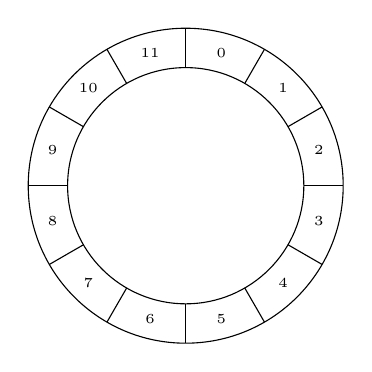
\begin{tikzpicture}[scale=.5]
				      \def\RayonListe{3}
				      \def\EpaisseurListe{1}
				      \def\LongueurListe{12}
				      \draw (0,0) circle(\RayonListe);
				      \draw (0,0) circle(\RayonListe+\EpaisseurListe);
				      \foreach \compt in {0,1,...,\numexpr\LongueurListe-1}
					      {
						      \draw (90-\compt/\LongueurListe*360:\RayonListe)--(90-\compt/\LongueurListe*360:\RayonListe+\EpaisseurListe);
						      \draw (90-\compt/\LongueurListe*360-180/\LongueurListe:\RayonListe+\EpaisseurListe/2)node{\tiny \compt};
					      }
			      \end{tikzpicture}
		      \end{center}
		      
		\item 	
		      Refaire \textbf{1.} et \textbf{2.} mais en sautant 5 cases.\\
		      Case parcourues : \dotfill
		      
		      \begin{center}
			      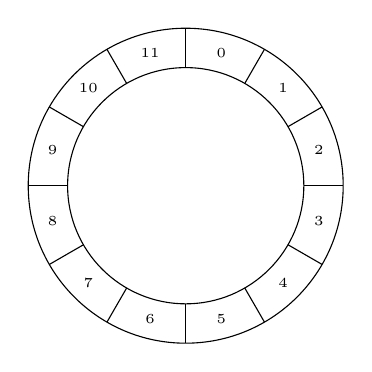
\begin{tikzpicture}[scale=.5]
				      \def\RayonListe{3}
				      \def\EpaisseurListe{1}
				      \def\LongueurListe{12}
				      \draw (0,0) circle(\RayonListe);
				      \draw (0,0) circle(\RayonListe+\EpaisseurListe);
				      \foreach \compt in {0,1,...,\numexpr\LongueurListe-1}
					      {
						      \draw (90-\compt/\LongueurListe*360:\RayonListe)--(90-\compt/\LongueurListe*360:\RayonListe+\EpaisseurListe);
						      \draw (90-\compt/\LongueurListe*360-180/\LongueurListe:\RayonListe+\EpaisseurListe/2)node{\tiny \compt};
					      }
			      \end{tikzpicture}
		      \end{center}
		\item 	Comment expliquer la différence entre la dernière liste et les deux premières ?
	\end{enumerate}
\end{exercice}


\begin{exercice}[]
	On parcourt une liste circulaire de longueur 84 comme à l'exercice précédent, en partant de la case d'indice zéro et en sautant 735 cases (et oui
	cela fait beaucoup) à chaque fois, indéfiniment.\\
	La liste sera-t-elle parcourue entièrement ? Si ce n'est pas le cas, donner la liste des cases parcourues.\\
	\textit{Justifier les réponses}.
\end{exercice}

\chapter{Logique propositionnelle}
\section{Notion de proposition}


\begin{definition}[ : proposition]
	Une proposition est un énoncé qui a un sens et pour lequel on peut dire avec certitude qu'il est vrai ou faux. On dit qu'on peut lui associer une \textit{valeur de vérité}. Cette valeur peut se noter \textsc{vrai} ou \textsc{faux} mais on peut aussi choisir de la noter 0 (pour faux) ou 1 (pour vrai).
\end{definition}
\begin{exemple}[s]
	\begin{itemize}
		\item 	« $2+2 = 5$ » est une proposition fausse.
		\item 	« $2+2\equiv 1\ [3]$ » est une proposition vraie.
	\end{itemize}
\end{exemple}

\begin{exercice}[]
	L'affirmation « Cette affirmation est fausse » est-elle une proposition ?
\end{exercice}
\section{Connecteurs logiques}
\begin{definition}[ : négation d'une proposition]
	L'opérateur de négation se note avec une barre $\barmaj{\ }$. C'est un opérateur \textit{unaire}, c'est à dire qu'il s'applique à \textit{une} proposition.\\
	Il est défini par la table de vérité suivante :
	\tabstyle[UGLiGreen]
	\begin{center}
		\begin{tabular}{|c|c|}
			\ccell $P$ & \ccell $\barmaj{ P}$ \\
			0          & 1                    \\
			1          & 0                    \\
		\end{tabular}
	\end{center}
	$\barmaj{P}$ se lit « non P ».
\end{definition}

\begin{definition}[ : conjonction de deux propositions]
	L'opérateur de \textit{conjonction} correspond au \texttt{and} de \textsc{Python}, au \texttt{And} de \textsc{Visual Basic}, au \texttt{\&\&} de \textsc{C++}.
	Il se note $\wedge$, c'est un opérateur \textit{binaire} car il s'applique à deux propositions.\\
	Il est défini par la table de vérité suivante :
	\begin{center}
		\tabstyled
		\begin{tabular}{|c|c|c|}
			\rowcolor{UGLiGreen}
			\ccell $P$ & \ccell $Q$ & \ccell $P\wedge Q$ \\
			
			
			0                  & 0                  & 0                          \\
			
			
			0                  & 1                  & 0                          \\
			
			
			1                  & 0                  & 0                          \\
			
			1                  & 1                  & 1                          \\
		\end{tabular}
	\end{center}
	$P\wedge Q$ se lit « P et Q » et n'est vrai que si P est vrai et Q aussi.
\end{definition}

\begin{definition}[ : disjonction de deux propositions]
	L'opérateur de \textit{disjonction} correspond au \texttt{or} de \textsc{Python}, au \texttt{Or} de \textsc{Visual Basic}, au \texttt{||} de \textsc{C++}.
	Il se note $\vee$, c'est un opérateur \textit{binaire}.	Il est défini par la table de vérité suivante :
	\begin{center}
		\tabstyled
		\begin{tabular}{|c|c|c|}
			
			\rowcolor{UGLiGreen}
			\ccell\boldmath$P$ & \ccell\boldmath$Q$ & \ccell\boldmath$P\vee Q$ \\
			
			\rowcolor{white}
			0                  & 0                  & 0                        \\
			
			\rowcolor{white}
			0                  & 1                  & 1                        \\
			
			\rowcolor{white}
			1                  & 0                  & 1                        \\
			
			1                  & 1                  & 1                        \\
		\end{tabular}
	\end{center}
	$P\vee Q$ se lit « P ou Q » et est vrai dès que P est vrai ou Q est vrai.
\end{definition}

\begin{definition}[ : équivalence de deux propositions]
	Il se note $\Leftrightarrow$, c'est un opérateur \textit{binaire}.
	Il est défini par la table de vérité suivante :
	\begin{center}
		\tabstyled
		\begin{tabular}{|c|c|c|}
			\rowcolor{UGLiGreen}
			\ccell $P$ & \ccell $Q$ & \ccell $P\Leftrightarrow Q$ \\
			0                  & 0                  & 1                                   \\
			0                  & 1                  & 0                                   \\
			1                  & 0                  & 0                                   \\
			1                  & 1                  & 1                                   \\
		\end{tabular}
	\end{center}
	$P\Leftrightarrow Q$ se lit « P équivaut à Q » et n'est vrai que si P et Q ont la même valeur de vérité.
\end{definition}


\begin{definition}[ : implication]
	Il se note $\Rightarrow$, c'est un opérateur \textit{binaire}.
	Il est défini par la table de vérité suivante :
	\begin{center}
		\tabstyled
		\begin{tabular}{|c|c|c|}
			\rowcolor{UGLiGreen}
			\ccell\boldmath$P$ & \ccell\boldmath$Q$ & \ccell\boldmath$P\Rightarrow Q$ \\
			0                  & 0                  & 1                               \\
			0                  & 1                  & 1                               \\
			1                  & 0                  & 0                               \\
			1                  & 1                  & 1                               \\
		\end{tabular}
	\end{center}
	$P\Rightarrow Q$ se lit « P implique Q ».
	\begin{itemize}
		\item 	Quand P est fausse, $P\Rightarrow Q$ est vraie : « le faux implique n'importe quoi ».
		\item 	Quand P est vraie, $P\Rightarrow Q$ n'est vraie que si Q est aussi vraie : « le vrai n'implique que le vrai ».
	\end{itemize}
\end{definition}

\begin{exercice}[]
	On note P et Q les affirmations suivantes :\\
	P = « Paul aime le foot  »\\
	Q = « Paul aime les maths  »\\
	Représenter les affirmations suivantes sous forme symbolique en utilisant P, Q et des
	connecteurs logiques.\\
	• A = « Paul aime le foot mais pas les maths  »\\
	• B = « Paul n'aime ni le foot, ni les maths »\\
	• C = « Paul aime le foot ou il aime les maths et pas le foot  »\\
	• D = « Paul aime les maths et le foot ou il aime les maths mais pas le foot  »\\
\end{exercice}

\begin{exercice}[]
	Donner les valeurs de vérité des propositions suivantes :\\
	• A = $(\pi = 5)\wedge(2 + 3 = 5)$\\
	• B = $(\pi = 5)\vee( 2 + 3 = 5)$\\
	• C = $(\pi=3,14)\Rightarrow (5+6=11)$\\
	• D = $(\pi=5)\Rightarrow(2 +3=5)$\\
	• E = $(4 = 5)\Rightarrow A$\\
	• F = $(5+5=10)\Leftrightarrow(\pi=11)$
\end{exercice}

\begin{exercice}[ (à faire plus tard)]
	Donner les valeurs de vérité des propositions suivantes :\\
	• A = $(11>0)\wedge(3<2)$\\
	• B = $(11>0)\vee( 3 <2)$\\
	• C = $(3>6)\vee (6>20)$\\
	• D = $(3<2)\Rightarrow(5=5)$\\
	• E = $(4 \neq 1)\Rightarrow (4=1)$\\
	• F = $(4<5)\Leftrightarrow(10+1=11)$
\end{exercice}


\begin{methode}[ : Montrer qu'une proposition est vraie]
	On peut montrer qu'une proposition composée est vraie en faisant prendre toutes les valeurs de vérités possibles aux propositions qui la compose et en trouvant sa table de vérité :\\
	
	Montrons que $(P\wedge Q)\Leftrightarrow(Q\wedge P)$ est vraie quelque soient les valeurs de vérité de P et de Q.
	
	\tabstyled
	\begin{center}
		\begin{tabular}{|c|c|c|c|c|}
			\rowcolor{UGLiPurple}
			\ccell\boldmath$P$ & \ccell\boldmath$Q$ & \ccell\boldmath$P\wedge Q$ & \ccell\boldmath$Q \wedge P$ & \ccell\boldmath$(P\wedge Q)\Leftrightarrow(Q\wedge P)$ \\
			0                  & 0                  & 0                          & 0                           & 1                                                      \\
			0                  & 1                  & 0                          & 0                           & 1                                                      \\
			1                  & 0                  & 0                          & 0                           & 1                                                      \\
			1                  & 1                  & 1                          & 1                           & 1                                                      \\
		\end{tabular}
	\end{center}
\end{methode}

\begin{exercice}[ : l'implication]
	Vérifier que la table de vérité de $P\Rightarrow Q$ est la même que celle de $\barmaj{P}\vee Q$.
\end{exercice}

\begin{exercice}[ : l'équivalence comme double implication]
	Vérifier que la table de vérité de $P\Leftrightarrow Q$ est la même que celle de $(P\Rightarrow Q)\wedge(Q\Rightarrow P)$.
\end{exercice}

\begin{exercice}[ : le ou exclusif]
	
	Notons $xor$ cet opérateur binaire. $P\ xor\ Q$ est vraie si (et seulement si) une et une seule des 2 propositions est vraie.
	\begin{enumerate}
		\item 	Donner la table de vérité de P xor Q.
		\item 	Vérifier que c'est la même que $(P\wedge \barmaj{Q})\vee(\barmaj{P}\wedge Q)$
		\item 	Vérifier que c'est la même que celle de $(P\vee Q)\wedge(\barmaj{P\wedge Q})$
	\end{enumerate}
\end{exercice}

\begin{exercice}[ : les lois de De Morgan]
	
	\begin{enumerate}
		\item 	Montrer que $\barmaj{P\wedge Q}\Leftrightarrow \barmaj{P} \vee \barmaj{Q}$
		\item 	Montrer que $\barmaj{P\vee Q}\Leftrightarrow (\barmaj{P} \wedge \barmaj{Q})$
	\end{enumerate}
\end{exercice}

\begin{propriete}[ : équivalences classiques]
	Les propositions suivantes sont vraies quelles que soient les valeurs de vérité de P, Q et R.\\
	On dit que ce sont des \textit{tautologies}.
	
	\begin{tabbing}
		$(P\wedge Q) \Leftrightarrow(Q\wedge P)$ 		\hspace{4cm}	\=commutativité de $\wedge$ \\
		$(P\vee Q) \Leftrightarrow(Q\vee P)$ 						 	\>commutativité de $\vee$ \\
		$((P\vee Q)\vee R) \Leftrightarrow(P\vee(Q\vee R))$ 			\>associativité de $\vee$ \\
		$((P\wedge Q)\wedge R) \Leftrightarrow(P\wedge(Q\wedge R))$ 	\>associativité de $\wedge$ \\
		$(P\wedge (Q\vee R))\Leftrightarrow((P\wedge Q)\vee(P\wedge R))$ \>distributivité de $\wedge$ sur $\vee$\\
		$(P\vee (Q\wedge R))\Leftrightarrow((P\vee Q)\wedge(P\vee R))$ \>distributivité de $\vee$ sur $\wedge$\\
		$(P\Rightarrow Q)\Leftrightarrow(\barmaj{P} \vee Q)$\\
		$\barmaj{P\wedge Q}\Leftrightarrow (\barmaj{P}\vee \barmaj{Q})$ \> loi de De Morgan\\
		$\barmaj{P\vee Q}\Leftrightarrow (\barmaj{P} \wedge \barmaj{Q})$ \> loi de De Morgan\\
	\end{tabbing}
\end{propriete}

\begin{exemple}[ : utilité de le proposition suivante]
	
	\begin{itemize}
		\item 	« Il viendra mardi et il apportera son PC ou bien il viendra mercredi et il apportera son PC »\\
		      se simplifie en :\\	« Il viendra mardi ou mercredi et il apportera son PC ».
		\item 	« On n'a pas :  Jean est gentil ou Jean est drôle » peut se réécrire :\\
		      « Jean n'est pas gentil et Jean n'est pas drôle ».
	\end{itemize}
\end{exemple}

\begin{exercice}[]
	Simplifier « On n'a pas : Pierre habite Saint Brieuc et Pierre est brun ».
\end{exercice}


\section{Calcul des prédicats}

\begin{definition}[s : quantificateurs, variables, prédicats]
	
	Le symbole $\forall$ se lit « pour tout » et s'appelle \textit{quantificateur universel}.\\
	Le symbole $\exists\,$ se lit « il existe » et s'appelle \textit{quantificateur existentiel}.\\
	
	Une \textit{variable} est un symbole qui peut prendre plusieurs valeurs.
	
	Un \textit{prédicat} est un énoncé sans valeur de vérité qui contient au moins une variable, et qui devient une proposition en ajoutant un ou des quantificateurs.
\end{definition}

\begin{exemple}[s]
	\begin{itemize}
		\item 	« $x<1$ » est un prédicat comportant une variable $x$.
		\item 	$\exists\, x\in R,\ x<1$ est une proposition. Cette proposition est vraie : il existe un nombre réel strictement plus petit que 1 (et même une infinité) : 0 par exemple.
		\item 	$\forall x\in\R,\ x<1$ est une autre proposition... fausse ! Tout nombre réel n'est pas strictement plus petit que 1 : 2 par exemple.
	\end{itemize}
\end{exemple}

\begin{propriete}[ : ordre des quantificateurs]
	Dans un prédicat à plusieurs variables, quand plusieurs quantificateurs de la même catégorie se suivent, on peut les échanger librement.\\
	On \textit{ne peut pas} échanger un quantificateur $\exists\,$ et un quantificateur $\forall$.
\end{propriete}

\begin{exemple}[s]
	\begin{itemize}
		\item 	$\forall x\in\R,\ \forall y\in\R,\ \exists\, z \in\R, x+y<z$ est une proposition vraie : pour tous réels x et y on peut prendre z égal à $x+y+1$.\\
		      On peut échanger les quantificateurs universels : $\forall y\in\R,\ \forall x\in\R,\ \exists\, z \in\R, x+y<z$ est équivalent à la proposition précédente.
		\item 	$\forall x\in\R,\ \exists\, y \in\R, x<y$ est une proposition vraie mais on ne peut pas échanger les quantificateurs : on obtient :
		      $\exists\, y\in\R,\ \forall x \in\R, x<y$ est fausse : cela voudrait dire qu'il existe un réel $y$ plus grand que tous les autres !
	\end{itemize}
\end{exemple}

\begin{propriete}[ : négation d'une proposition quantifiée]
	On obtient la négation d'une proposition quantifiée en changeant les $\exists\,$ en $\forall$, les $\forall$ en $\exists\,$ et en changeant le prédicat final par sa négation.
\end{propriete}

\begin{exemple}[]
	On considère la propriété P : $$\forall n\in\N,\ \exists\, k\in\N,\ n=2k$$
	Sa négation est $\barmaj{P}$ :  $$\exists\, n\in\N,\ \forall k\in\N,\ n\neq 2k$$
	P est fausse puisqu'elle affirme que tout entier naturel est divisible par 2 !\\ Sa négation est vraie : elle affirme qu'il existe un entier naturel qui n'est pas divisible par 2 (3 par exemple).
\end{exemple}

\begin{methode}[s : preuve de propositions quantifiées]
	\begin{itemize}
		\item 	Pour prouver qu'une proposition quantifiée par $\forall$ est fausse, il suffit de donner un \textit{contre exemple}.
		\item 	Pour prouver qu'une proposition quantifiée par $\exists\, x...$ est vraie, on peut déterminer la valeur de $x$ qui convient.
		\item 	Pour prouver qu'une proposition quantifiée par $\forall$ est vraie on a souvent recours à un raisonnement ou au calcul littéral.
		\item 	De même pour prouver qu'une proposition quantifiée par $\exists\, x...$ est fausse.
	\end{itemize}
\end{methode}

\begin{exemple}[s]
	\begin{itemize}
		\item 	Montrons que $\forall x \in \R,\ \exists\, y\in \R,\ 3y+1=x$ :\\
		      Soit $x\in\R$ alors $3y+1=x\Leftrightarrow y=\frac{1}{3}(x-1)$. Donc  $\frac{1}{3}(x-1)$ convient.
		\item 	Montrons que $\forall x\in\R,\ \exists\, y\in\R,\ x=y^2$ est fausse :\\
		      Prenons $x=-1$. Il n'existe aucun $y\in\R$ tel que $x=y^2$. En effet d'après la règle des signes, $y^2$ est obligatoirement positif.
	\end{itemize}
\end{exemple}

\begin{exercice}[]
	Vrai ou faux ? Justifier.
	\begin{itemize}
		\item 	$\forall n \in \N,\ \forall p \in \N,\ p-n \equiv 0\ [2]$
		\item 	$\forall n \in \N,\ \exists\, p \in \N,\ p-n \equiv 0\ [2]$
		\item 	$\exists\, n \in \N,\ \exists\, p \in \N,\ p-n \equiv 0\ [2]$
		\item 	$\exists\, n \in \N,\ \forall p \in \N,\ p-n \equiv 0\ [2]$
	\end{itemize}
\end{exercice}

\begin{exercice}[]
	Donner les négations des propositions suivantes et dire laquelle est vraie : la proposition ou sa négation.
	\begin{itemize}
		\item 	$\exists\, x\in\R,\ 3x=2$
		\item 	$\forall x\in\R,\ x=x+1$
		\item 	$\forall x\in\R,\ \forall y\in\R, x\leqslant y$
		\item 	$\exists\, x\in\R,\ \forall y\in\R,\ x^2=y$
		\item 	$\forall x\in\R,\ \exists\, y\in\R,\ x^2=y$
	\end{itemize}
\end{exercice}


\section{Exercices}


\begin{exercice}

	En utilisant les tables de vérités, montrer que, quelles que soient les valeurs de vérité de P et Q, on a $$\barmaj{P} \wedge \barmaj{Q} \Leftrightarrow \barmaj{P\vee Q}$$
	
	Compléter
	
	\begin{center}
		\tabstyled
		\begin{tabular}{|c|c|c|c|c|c|c|}
			
			\ccell $P$ & \ccell $Q$ & \ccell$\barmaj{P}$ & \ccell$\barmaj{Q}$ & \ccell$\barmaj{P} \wedge \barmaj{Q}$ & \ccell$P\vee Q$ & \ccell$\barmaj{P\vee Q}$ \\
			         &          &                    &                    &                                      &                 &                          \\
			         &          &                    &                    &                                      &                 &                          \\
			         &          &                    &                    &                                      &                 &                          \\
			         &          &                    &                    &                                      &                 &                          \\
		\end{tabular}
	\end{center}
	Indiquer les colonnes identiques qui permettent de conclure.
\end{exercice}

\begin{exercice}
	En utilisant les tables de vérités, montrer que, quelles que soient les valeurs de vérité de P et Q, on a $$(P\vee Q)\wedge (P\vee \barmaj{Q})\Leftrightarrow P$$
	
	Compléter
	
	\begin{center}
		\tabstyled
		\begin{tabular}{|c|c|c|c|c|c|c|}
			
			\ccell $P$ & \ccell $Q$ & \ccell$\barmaj{P}$ & \ccell$\barmaj{Q}$ & \ccell$P \vee Q$ & \ccell$P\vee \barmaj{Q}$ & \ccell$(P\vee Q)\wedge (P\vee \barmaj{Q})$ \\
			
			         &          &                    &                    &                  &                          &                                            \\
			
			         &          &                    &                    &                  &                          &                                            \\
			
			         &          &                    &                    &                  &                          &                                            \\
			
			         &          &                    &                    &                  &                          &                                            \\
		\end{tabular}
	\end{center}
	Indiquer les colonnes identiques qui permettent de conclure.
\end{exercice}

\begin{exercice}[ : lois de De Morgan]
	En utilisant des tables de vérité, montrer que, quelles que soient les valeurs de vérité de P et Q, on a $$\barmaj{P\vee Q}=\barmaj{P}\wedge\barmaj{Q}$$
	De même  montrer que $$\barmaj{P\wedge Q}=\barmaj{P}\vee\barmaj{Q}$$
\end{exercice}
\begin{exercice}[ : on peut retrouver tous les opérateurs à partir du nor]
	
	Pour toutes propositions $A$ et $B$ on définit l'opération  «  nor » , notée $\downarrow$ par : $$A\downarrow B \Longleftrightarrow\barmaj{A\vee B}$$
	
	Cette opération est dite \textit{universelle} car elle permet de retrouver toutes les autres opérations.
	
	\begin{enumerate}
		\item 	Montrer que $A\downarrow A \Longleftrightarrow \barmaj{A}$ (on peut donc retrouver l'opération « non »).
		\item 	En déduire que l'on peut retrouver l'opération « et » ainsi : $$(A\downarrow B)\downarrow(A\downarrow B) = A\vee B$$
		\item 	Comment à partir de $A$, $B$ et $\downarrow$ obtenir $A\wedge B$ (penser aux lois de De Morgan) ?
	\end{enumerate}
\end{exercice}

\begin{exercice}

	Sans chercher à démontrer quoi que ce soit, donner les négations des propositions suivantes
	
	\begin{enumerate}
		\item 	$\forall x\in \R,\, \forall y\in\R,\, \exists\, z\in \R,\, x<z<y$
		\item 	$\exists\, x\in \R,\, \exists\, y\in\R,\, x+y>3$
		\item 	$\forall n\in \N^*,\, \exists\, p\in\N^*$ n divise p ou p divise n.
	\end{enumerate}
	
\end{exercice}

\begin{exercice}
	\begin{enumerate}
		\item 	A : $\forall n \in \N$ 3 divise n ou 2 divise n\\
		      Montrer que A est fausse
		\item 	B : $\exists\, n \in \N$, 3 divise n et 4 divise n\\
		      Montrer que B est vraie
		\item 	C :  «  Quand on prend trois nombres entiers qui se suivent, leur somme est toujours un multiple de 3  » .\\
		      Montrer que C est vraie.
		      
		\item 	D :  «  Quand on prend quatre nombres entiers qui se suivent, leur somme est toujours un multiple de 4  » .\\
		      Montrer que D est fausse.
		\item 	E :  «  Il existe deux entiers k et n plus grands que 1 tels que k divise à la fois n et n+1.\\
		      Montrer que E est fausse.
	\end{enumerate}
\end{exercice}

\chapter{Matrices}
\section{Notion de matrice}
\begin{definition}[ : matrice]
	Une matrice $A$ peut être vue comme « un tableau de nombres ».\\
	Supposons qu'elle comporte n lignes et p colonnes (n et p sont des entiers plus grands que 1), on la note ainsi
	$$A = \begin{matrice}
			a_{11}      & a_{12}&\cdots & a_{1p} \\
			a_{21}  & a_{22}& \cdots & a_{2p} \\
			\vdots 	& \vdots & \ddots & \vdots \\
			a_{n1}  & a_{n2}    & \cdots & a_{np}
		\end{matrice}$$
	L'élément qui se situe à la i\eme ligne et à la j\eme colonne est noté $a_{ij}$. On l'appelle également \textit{coefficient}.\\
	
	\textbf{Attention} : les indices des lignes et des colonnes commencent à 1 (et non à zéro comme dans la plupart des langages informatiques).\\
	
	Pour résumer l'écriture précédente on écrit
	$$A=(a_{ij})_{\substack{1\leqslant i\leqslant n\\1\leqslant j\leqslant p}}$$
	
	On dit aussi que $A$ est une matrice $n\times p$. Si $n=p$ on dit que $A$ est une \textit{matrice carrée d'ordre $n$}.
\end{definition}

\begin{exemple}[s]
	\begin{itemize}
		\item 	$B =	\begin{matrice}
				      1      & 2 & 4 \\
				      -3  & 5 & 0
			      \end{matrice}$ est une matrice à 2 lignes et 3 colonnes. On a $b_{21}=-3$.
		\item 	$C =	\begin{matrice}
				      2,4      & 7 & 4 & -1 \\
				      -3  & 5 & 10,1 & 1 \\
				      0,01 & 3 & 12 & 100
			      \end{matrice}$ est une matrice à 3 lignes et 4 colonnes. On a $c_{33}=12$.
		\item 	$D =	\begin{matrice}
				      4      & 2\\
				      2  &8
			      \end{matrice}$ est une matrice carrée d'ordre 2.
		      
		      
	\end{itemize}
\end{exemple}

\begin{exercice}[]
	On considère 	$E =	\begin{matrice}
			-4      & 7,6 & 4 & -1 & 12 \\
			8 & -3  & 5,7 & 101 & 1 \\
			12 & 0,01 & 3 & 12 & 1
		\end{matrice}$.\\
	
	Donne les valeurs de $e_{12}$, $e_{21}$, $e_{35}$ et $e_{24}$.
\end{exercice}

Le script \textsc{Python} suivant permet de générer une matrice $n\times p$ avec des coefficients entiers aléatoires compris entre -100 et 100.

\begin{pyc}
	\begin{minted}{python}
		from random import randint

		n = int(input("Entrez le nombre de lignes : "))
		p = int(input("Entrez le nombre de colonnes : "))

		matrice = []  # une matrice est une liste de lignes

		for i in range(n):  # il y a n lignes
			ligne = []  # on construit une ligne vide
			for j in range(p):  # il y a p colonnes
				ligne.append(randint(-100, 100))  # on remplit la ligne aléatoirement
			matrice.append(ligne)  # on ajoute la ligne à la liste de lignes
	\end{minted}
\end{pyc}
\begin{exercice}[]
	\begin{enumerate}
		\item \'Ecris complètement la matrice suivante : $M=(m_{ij})_{\substack{1\leqslant i\leqslant 3\\1\leqslant j\leqslant 5}}$ où $m_{ij}=i$ si i=j et 0 sinon.
		\item 	\'Ecris complètement la matrice suivante : $M=(m_{ij})_{\substack{1\leqslant i\leqslant 4\\1\leqslant j\leqslant 5}}$ où $m_{ij}=0$ si i<j et 1 sinon.
		\item 	\'Ecris complètement la matrice suivante : $M=(m_{ij})_{\substack{1\leqslant i\leqslant 3\\1\leqslant j\leqslant 3}}$ où $m_{ij}=1$ si $i+j$ est pair et 0 sinon.
		\item \textsc{bonus} : écris des programmes \textsc{Python} qui génèrent ces matrices.
	\end{enumerate}
\end{exercice}

\begin{definition}[s : Matrices nulles et identités]
	\begin{itemize}
		\item 	Une matrice dont tous les coefficients sont nuls est dite \textit{nulle} (c'est « un tableau de zéros »);
		\item 	la matrice \textit{carrée d'ordre $n$} dont tous les éléments sont nuls sauf ceux de la \textit{diagonale} (c'est-à-dire ceux qui s'écrivent $a_{ii})$ qui valent 1 s'appelle \textit{la matrice identité d'ordre $n$} et se note $I_n$.
	\end{itemize}
\end{definition}

\begin{exemple}[]
	La matrice identité $I_3$ est
	$I_3= \begin{matrice}
			1&0&0\\
			0&1&0\\
			0&0&1
		\end{matrice}$.
\end{exemple}

\section{Opérations sur les matrices}

\begin{definition}[ : addition]
	Soient $A$ et $B$ deux matrices $n\times p$, on note $A+B$ la matrice $n\times p$ obtenu en ajoutant les coefficients correspondants de $A$ et de $B$ :
	
	$$\begin{matrice}
			a_{11}      & \cdots & a_{1p} \\
			
			\vdots 	& \ddots & \vdots \\
			a_{n1}      & \cdots & a_{np}
		\end{matrice} +\begin{matrice}
			b_{11}      & \cdots & b_{1p} \\
			
			\vdots 	& \ddots & \vdots \\
			b_{n1}      & \cdots & b_{np}
		\end{matrice}=
		\begin{matrice}
			a_{11} +b_{11}     & \cdots & a_{1p}+b_{1p} \\
			
			\vdots 	& \ddots & \vdots \\
			a_{n1}+n_{n1}      & \cdots & a_{np}+b_{np}
		\end{matrice}$$
\end{definition}

\begin{exemple}[]
	Prenons $A = \begin{matrice}
			3&1\\
			4&7\\
			-2&8
		\end{matrice}$ et $B = \begin{matrice}
			2&5\\
			1&-3\\
			-5&9
		\end{matrice}$, alors $A+B=\begin{matrice}
			5&6\\5&4\\-7&17
		\end{matrice}$.\end{exemple}
\begin{remarque}[]
	\textbf{Attention :} on ne peut ajouter deux matrices que si elles ont les mêmes dimensions (c'est-à-dire même nombre de lignes et même nombre de colonnes).
\end{remarque}
\begin{definition}[ : multiplication par un réel]
	Soient $A$ une matrice $n\times p$ et $k$ un nombre réel, on note $kA$ la matrice $n\times p$ obtenue en multipliant chaque coefficient de $A$ par $k$ :
	
	$$k\begin{matrice}
			a_{11}      & \cdots & a_{1p} \\
			\vdots 	& \ddots & \vdots \\
			a_{n1}      & \cdots & a_{np}
		\end{matrice}=\begin{matrice}
			k\times a_{11}      & \cdots & k\times a_{1p} \\
			\vdots 	& \ddots & \vdots \\
			k\times a_{n1}      & \cdots &k\times a_{np}
		\end{matrice}
	$$
\end{definition}

\begin{exemple}[]
	Prenons $A = \begin{matrice}
			8&3&1\\
			4&7&2\\
			-2&1&8
		\end{matrice}$ et $k=5$, alors on obtient que $5A = \begin{matrice}
			40&15&5\\
			20&35&10\\
			-10&5&40
		\end{matrice}$.\end{exemple}


La propriété suivante énonce quelques résultats utiles pour calculer.
\begin{propriete}[ : règles de calcul]
	Soient $A$, $B$ et $C$ trois matrices de mêmes dimensions et $k$ et $k'$ 2 réels.
	\begin{itemize}
		\item 	$A+B = B+A$
		\item 	$(A+B)+C = A+(B+C)$
		\item 	$k(A+B) = kA + kB$
		\item 	$(k+k')A = kA+k'A$
	\end{itemize}
\end{propriete}

\begin{exercice}[]
	On pose $A=\begin{matrice}
			1&2\\3&-4
		\end{matrice}$, $B=\begin{matrice}
			11&10\\-9&7
		\end{matrice}$ et $C=\begin{matrice}
			-3&-2\\5&-5
		\end{matrice}$.\\
	
	Montrer que $B-2A+3C$ est une matrice nulle.
\end{exercice}

\begin{definition}[ : multiplication de deux matrices]
	
	Soient $A$ une matrice $n\times p$ et $B$ une matrice $p\times q$ (le nombre de colonnes de la 1\ere est égal au nombre de lignes de la 2\eme) alors il est possible de définir la matrice $C=A\times B$, produit de $A$ par $B$.\\
	C'est une matrice $n\times q$ dont les coefficients sont ainsi :
	\begin{center}
		\begin{tabular}{cc}
			                                                                                                                                    & $\begin{matrice}
					                                                                                                                                       b_{11}   &\cdots   &\cellcolor{lightgray!50}\color{UGLiOrange}b_{1j}& \cdots & a_{1q} \\
					                                                                                                                                       \vdots 	& \ddots &\cellcolor{lightgray!50}\color{UGLiOrange}\cdots&\dots & \vdots \\
					                                                                                                                                       b_{k1} & \cdots & \cellcolor{lightgray!50}\color{UGLiOrange}b_{kj}&\cdots & b_{kq}\\
					                                                                                                                                       \vdots 	& \cdots &\cellcolor{lightgray!50}\color{UGLiOrange}\cdots&\ddots & \vdots \\
					                                                                                                                                       b_{p1}    &\cdots  &\cellcolor{lightgray!50}\color{UGLiOrange}b_{pj} & \cdots &b_{pq}
				                                                                                                                                       \end{matrice}$ \\
			
			$\begin{matrice}
					 a_{11}   &\cdots   &\cdots& \cdots & a_{1p} \\
					 \vdots 	& \ddots &\cdots&\dots & \vdots \\
					 \rowcolor{lightgray!50} \color{UGLiGreen}    a_{i1} & \color{UGLiGreen}\cdots &\color{UGLiGreen} a_{ik}&\color{UGLiGreen}\cdots & \color{UGLiGreen}a_{ip}\\
					 \rowcolor{white}\vdots 	& \cdots &\cdots&\ddots & \vdots \\
					 a_{n1}    &\cdots  & \cdots & \cdots &a_{np}
				 \end{matrice}$ & 
			$\begin{matrice}
					 c_{11}   &\cdots   &\cdots& \cdots & c_{1q} \\
					 \vdots 	& \ddots &\cdots&\dots & \vdots \\
					 \vdots & \cdots &\cellcolor{lightgray!50} \color{UGLiRed}c_{ij}&\cdots & \vdots\\
					 \vdots 	& \cdots &\cdots&\ddots & \vdots \\
					 c_{n1}    &\cdots  & \cdots & \cdots &c_{nq}
				 \end{matrice}$
		\end{tabular}
	\end{center}
	{\LARGE$$ {\color{UGLiRed}c_{ij}} = {\color{UGLiGreen}a_{i1}}\times {\color{UGLiOrange}b_{1j}}+ {\color{UGLiGreen}a_{i2}}\times {\color{UGLiOrange}b_{2j}}+\ldots+ {\color{UGLiGreen}a_{ip}}\times {\color{UGLiOrange}b_{pj}}$$}
\end{definition}

\begin{exemple}[]
	
	Prenons $A=\begin{matrice}
			1&3 & -2 \\5 &-3&4
		\end{matrice}$ et $B=\begin{matrice}
			-5 & 1 & 0 & 2\\2& 1 & -1 & -8\\3 &4 & 0 & 9
		\end{matrice}$ alors $A$ est une matrice $2\times 3$, $B$ est une matrice $3\times 4$ donc il est possible de définir la matrice $C=A\times B$, ce sera une matrice $2\times 4$.
	\begin{center}
		\begin{tabular}{cc}
			                                                                      & $\begin{matrice}
					                                                                         -5 & 1 & \color{UGLiOrange}0 & 2\\2& 1 & \color{UGLiOrange}-1 & -8\\3 &4 & \color{UGLiOrange}0 & 9
				                                                                         \end{matrice}$ \\
			$\begin{matrice}
					 1&3 & -2 \\\color{UGLiGreen}5 &\color{UGLiGreen}-3&\color{UGLiGreen}4
				 \end{matrice}$ & $\begin{matrice}
					                   -5&-4&-3&-40\\-19&18&\color{UGLiRed}3&70
				                   \end{matrice}$
		\end{tabular}
	\end{center}
	Par exemple, pour calculer $c_{33}$, on fait ${\color{UGLiGreen}5}\times {\color{UGLiOrange}0}+ {\color{UGLiGreen}(-3)}\times {\color{UGLiOrange}(-1)}+ {\color{UGLiGreen}4}\times {\color{UGLiOrange}0}={\color{red}3} $.
\end{exemple}

\begin{remarque}[]
	\textbf{Attention :}
	\begin{itemize}
		\item 	on ne peut multiplier $A$ par $B$ que si le nombre de colonnes de $A$ est égal au nombre de lignes de $B$;
		\item 	ce n'est pas parce qu'on peut calculer $A\times B$ qu'on peut calculer $B\times A$ : les matrices de l'exemple précédent ne permettent pas de calculer $B\times A$ car le nombre de colonnes de $B$ n'est pas égal au nombre de lignes de $A$:
		      \begin{center}
			      \begin{tabular}{cc}
				                                                                                                         & $\begin{matrice}
						                                                                                                            1&3 & -2 \\\color{UGLiGreen}5 &\color{UGLiGreen}-3&\color{UGLiGreen}4
					                                                                                                            \end{matrice}$ \\
				      $\begin{matrice}
						       -5 & 1 & \color{UGLiOrange}0 & 2\\2& 1 & \color{UGLiOrange}-1 & -8\\3 &4 & \color{UGLiOrange}0 & 9
					       \end{matrice}$ & Impossible
			      \end{tabular}
		      \end{center}
		\item pour pouvoir calculer $A\times B$ et $B\times A$ il faut que ces deux matrices soient carrées d'ordre $n$ et \textit{en général} on n'a pas $A\times B=B\times A$.
	\end{itemize}
\end{remarque}

\begin{exercice}[]
	\begin{itemize}
		\item 	On pose $A=\begin{matrice}
				      1&2\\3&0
			      \end{matrice}$ et $B=\begin{matrice}
				      5&2\\0&3
			      \end{matrice}$.\\
		      
		      Calculer $AB$ et $BA$.
		      
		\item 	Recommencer avec $A=\begin{matrice}
				      -4&6\\-3&5
			      \end{matrice}$ et $B=\begin{matrice}
				      8&-10\\5&-7
			      \end{matrice}$.
	\end{itemize}
\end{exercice}

\begin{propriete}[s de calcul]
	
	$A$, $B$ et $C$ sont des matrices.\\
	Lorsque les opérations sont possibles (bonnes dimensions des matrices) on a :
	\begin{itemize}
		\item 	$A(BC)=(AB)C$;
		\item 	$(A+B)C=AC+BC$;
		\item 	$A(B+C)=AB+AC$.\\
	\end{itemize}
	Soit $k$ un nombre réel alors on a également $A\times kB=kAB$.\\
	
	Si $A$ est \textit{carrée d'ordre} $n$ on a
	\begin{itemize}
		\item 	$AI_n=I_nA=A$ où $I_n$ est la matrice identité d'ordre $n$.
		\item 	$A\times 0=0\times A=0$ en notant 0 la matrice carrée d'ordre $n$ nulle.
	\end{itemize}
\end{propriete}

\section{Exemple concret d'utilisation}

Imaginons une école qui forme des ingénieurs en informatique, avec seulement 3 matières.
Trois élèves de première année ont obtenu les résultats suivants :

\begin{center}
	\textbf{Résultats pour le premier trimestre}\\[1em]
	\tabstyle[UGLiBlue]
	\begin{tabular}{|c|c|c|c|c|}
		\hline
		\bcell   & \ccell Maths & \ccell Physique & \ccell Info \\
		\hline
		Adam     & 12           & 8               & 16          \\
		\hline
		Bertrand & 18           & 14              & 12          \\
		\hline
		Charles  & 5            & 20              & 15          \\
		\hline
	\end{tabular}\\
	
	\textbf{Résultats pour le deuxième trimestre}\\[1em]
	
	\begin{tabular}{|c|c|c|c|c|}
		\hline
		\bcell   & \ccell Maths & \ccell Physique & \ccell Info \\
		\hline
		Adam     & 10           & 10              & 14          \\
		\hline
		Bertrand & 18           & 12              & 14          \\
		\hline
		Charles  & 7            & 14              & 17          \\
		\hline
	\end{tabular}
\end{center}

Ces deux tableaux peuvent s'écrire matriciellement
$S_1= \begin{matrice}
		12 & 8 & 16 \\
		18 & 14 & 12 \\
		5 & 20 & 15 \\
	\end{matrice}$
et $S_2= \begin{matrice}
		10 & 10 & 14 \\
		18 & 12 & 14 \\
		7 & 14 & 17 \\
	\end{matrice}$\\

Pour calculer les moyennes mensuelles des élèves « en une fois » on peut définir $M=0,5(S_1+S_2)$:

$$M = 0,5 \times \left[\begin{matrice}
			12 & 8 & 16 \\
			18 & 14 & 12 \\
			5 & 20 & 15 \\
		\end{matrice}+\begin{matrice}
			10 & 10 & 14 \\
			18 & 12 & 14 \\
			7 & 14 & 17 \\
		\end{matrice}\right]$$

$$M = 0,5\times \begin{matrice}
		22 & 18 & 30 \\
		36 & 16 & 26 \\
		12 & 34 & 32 \\
	\end{matrice}$$

$$M = \begin{matrice}
		11 & 9 & 15 \\
		18 & 8 & 13 \\
		6 & 17 & 16 \\
	\end{matrice}$$

Le coefficient des mathématiques est 1, celui de la physique est 2 et celui de l'informatique est 5.\\
Pour passer en deuxième année, il faut un total de points supérieur ou égal à 120.

Pour faire « d'un coup » le total des points, on peut considérer la matrice de coefficients $C=\begin{matrice}
		1\\2\\5
	\end{matrice}$.\\

Les points des élèves sont donnés par la matrice $$P=MC$$
$$P = \begin{matrice}
		11 & 9 & 15 \\
		18 & 8 & 13 \\
		6 & 17 & 16 \\
	\end{matrice}\begin{matrice}
		1\\2\\5
	\end{matrice}$$

$$P = \begin{matrice}
		104\\109\\120\\
	\end{matrice}$$

Ainsi seul Charles est admis à passer en 2\eme année.

\section{Matrices inversibles et systèmes}

\begin{definition}[ et propriété : Matrice inversible, inverse d'une matrice]
	Soit $A$ une matrice \textbf{carrée d'ordre $n$}. S'il existe une matrice $B$ d'ordre $n$ telle que
	$$AB = I_n\qquad\text{ou}\qquad BA=I_n$$
	
	alors automatiquement les deux égalités sont vérifiées, $B$ est nécessairement \textit{unique} et on dit alors que $B$ \textit{est l'inverse de $A$}. De manière symétrique $A$ est également l'inverse de $B$ si bien qu'on dit que $A$ et $B$ sont inverses l'une de l'autre.
	
	On note ceci $A=B^{-1}$ ou, ce qui revient au même, $B=A^{-1}$.
\end{definition}

\begin{exemple}[]
	$A=\begin{matrice}
			-1&2\\-2&3
		\end{matrice}$ et $B=\begin{matrice}
			3&-2\\2&-1
		\end{matrice}$ sont inverses l'une de l'autre :
	\begin{center}
		\begin{tabular}{cc}
			 & $\begin{matrice}
					    3&-2\\2&-1
				    \end{matrice}$ \\
			$\begin{matrice}
					 -1&2\\-2&3
				 \end{matrice}$
			 & $\begin{matrice}
					    1&0\\0&1
				    \end{matrice}$
		\end{tabular}
	\end{center}
\end{exemple}
\begin{exercice}[]
	Montrer que $A=\begin{matrice}
			3 & -2&1\\
			-2&2&-1\\
			1&-1&1
		\end{matrice}$ et
	$B=\begin{matrice}
			1& 1&0\\
			1&2&1\\
			0&1&2
		\end{matrice}$ sont inverses.
	
\end{exercice}
\begin{remarque}[]
	Il existe des matrices non inversibles, par exemple $\begin{matrice}
			1 & 2\\ 2 & 4
		\end{matrice}$.
\end{remarque}


\newcolumntype{C}{>{{}}c<{{}}} % for columns with binary operators
\renewcommand\vv{\multicolumn{1}{c}{\vdots}}
\begin{methode}[ : résoudre des systèmes avec des matrices]
	On considère un \textit{système de $n$ équations à $n$ inconnues} :
	
	$$\left\lbrace
		\setlength{\arraycolsep}{0pt}
		\begin{array}{c<{x_1} C c<{x_2} C c C c<{x_n} C l}
			a_{11} & + & a_{12} & + & \cdots & + & a_{1n} & = & b_1    \\
			a_{21} & + & a_{22} & + & \cdots & + & a_{2n} & = & b_2    \\
			\vv    &   & \vv    &   &        &   & \vv    &   & \vdots \\
			a_{n1} & + & a_{n2} & + & \cdots & + & a_{nn} & = & b_n    \\
		\end{array}\right.$$
	
	On connaît tous les nombres $a_{ij}$ et tous les $b_i$, et on veut trouver les valeurs des inconnues $x_i$.\\
	
	Ce système peut se réécrire de manière matricielle :
	
	$$\begin{matrice}
			a_{11}      & a_{12}&\cdots & a_{1n} \\
			a_{21}  & a_{22}& \cdots & a_{2n} \\
			\vdots 	& \vdots & \ddots & \vdots \\
			a_{n1}  & a_{n2}    & \cdots & a_{nn}
		\end{matrice}
		\begin{matrice}
			x_{1}       \\
			x_2\\
			\vdots \\
			x_n
		\end{matrice}
		=\begin{matrice}
			b_{1}       \\
			b_2\\
			\vdots \\
			b_n
		\end{matrice}$$
	
	Ou encore :
	$$AX=B$$
	
	Si la matrice $A$ est inversible (en pratique ce sera toujours le cas parce qu'on nous donnera sa matrice inverse ou bien parce qu'on l'aura déterminée à l'aide de la calculatrice) alors, on peut reprendre l'égalité précédente et écrire : $A^{-1}AX=A^{-1}B$, ce qui donne $I_nX=A^{-1}B$. En définitive on a $$X = A^{-1}B$$
	
	Ainsi pour trouver les valeurs des inconnues $x_i$, on effectue simplement le produit matriciel $A^{-1}B$ : chacune de ses lignes nous donne la valeur du $x_i$ correspondant.
\end{methode}

\begin{remarque}[]
	Pour savoir comment utiliser la calculatrice, regarder ici :
	\begin{itemize}
		\item 	modèles \textsc{CASIO} \texttt{https://youtu.be/yjvQx13Vhlk}
		\item 	modèles \textsc{Texas Instrument} \texttt{https://youtu.be/rxDxBnIwaGo}
	\end{itemize}
\end{remarque}

\begin{exemple}[]
	On considère le système suivant : \systeme{2x+5y+2z=1,
		5x-3y-2z=2,
		-x+2y+z=-3}\\
	
	Il peut se réécrire de manière matricielle :
	
	$$\begin{matrice}
			2 & 5 & 2 \\
			5 & -3 & -2\\
			-1 & 2 & 1
		\end{matrice}
		\begin{matrice}
			x \\ y \\ z
		\end{matrice}=
		\begin{matrice}
			1 \\ 2 \\ -3
		\end{matrice}$$
	
	Appelons $A$ la matrice carrée du membre de gauche. On détermine que $A$ est inversible avec la calculatrice et que son inverse est
	$$A^{-1}=\begin{matrice}
			1 & -1 & -4 \\
			-3 & 4 & 14\\
			7 & -9 & -31
		\end{matrice}$$
	On a donc
	
	$$\begin{matrice}
			x \\ y \\ z
		\end{matrice}=\begin{matrice}
			1 & -1 & -4 \\
			-3 & 4 & 14\\
			7 & -9 & -31
		\end{matrice}\begin{matrice}
			1 \\ 2 \\ -3
		\end{matrice}$$
	C'est à dire, en effectuant le produit dans le membre de droite
	
	$$\begin{matrice}
			x \\ y \\ z
		\end{matrice}=\begin{matrice}
			11\\-37\\82
		\end{matrice}$$
	
	On a donc résolu le système : \systeme{x=11,y=-37,z=82}
\end{exemple}
\begin{exercice}[]
	\begin{enumerate}
		\item 	Effectue le produit suivant : $\begin{matrice}
				      1 & 2 \\ -3 & 3\end{matrice}\begin{matrice}x\\y\end{matrice}$.
		\item 	\'A l'aide de la calculatrice détermine l'inverse de la matrice $\begin{matrice}
				      1 & 2 \\ -3 & 3\end{matrice}$.
		\item Résous le système suivant : \systeme{x+2y = 15,-3x+3y = -6}
	\end{enumerate}
\end{exercice}


\section{Exercices}

\begin{exercice}

	Dans un parc d’une ville, deux marchands ambulants vendent des beignets,
	des crêpes et des gaufres. On a noté les ventes de chacun pour samedi et dimanche derniers.
	
	\begin{center}
		Marchand 1\\[1em]
		\tabstyled
		\begin{tabular}{|c|c|c|c|}
			\hline
			\bcell   & \ccell beignets & \ccell crêpes & \ccell gaufres \\
			\hline
			samedi   & 20              & 36            & 12             \\
			\hline
			dimanche & 26              & 40            & 18             \\
			\hline
		\end{tabular}\ \\[2em]
		
		Marchand 2\\[1em]
		
		\begin{tabular}{|c|c|c|c|}
			\hline
			\bcell   & \ccell beignets & \ccell crêpes & \ccell gaufres \\
			\hline
			samedi   & 30              & 40            & 22             \\
			\hline
			dimanche & 30              & 48            & 38             \\
			\hline
		\end{tabular}
	\end{center}
	
	
	On peut retenir l’information donnée par un tableau en conservant uniquement les
	nombres disposés de la même façon. On représente le 1er tableau par la matrice A :
	$$A=\begin{matrice}
			20&36&12\\
			26&40&18
		\end{matrice}$$
	
	\begin{enumerate}
		\item 	Donner la matrice B représentant le deuxième tableau.
		\item 	Que valent $a_{12}$, $a_{11}$, $a_{23}$ et $b_{11}$ ?
		\item 	Calculer $A+B$ et donner la signification de la matrice.
		\item 	Calculer $A-B$ et donner la signification de la matrice.
		\item  	Samedi et dimanche prochains, weekend de fête, on prévoit que les ventes vont augmenter de 50\%.\\
		      Par quel nombre k faut-il multiplier chacune des ventes du 1\er marchand ? \'Ecrire la matrice  kA.\\
		      Donner la matrice kB correspondant aux ventes du 2\eme marchand.
		\item 	Un beignet est vendu 2 euros, une crêpe 1 euro et une gaufre 1,50 euro.\\
		      On note V la matrice des prix de vente
		      $$V=\begin{matrice}
				      2\\
				      1\\
				      1,5
			      \end{matrice}$$
		      Quelle opération matricielle donne le montant des ventes par jour pour le 1\er marchand ? Pour le 2\eme ?
		\item 	 Les deux marchands travaillent pour le compte du même patron, qui leur demande	de calculer les coûts d’achats et les revenus pour chaque jour. Le coût d’achat d’un
		      beignet est 0,40 euro, d’une crêpe 0,25 euro, d’une gaufre 0,30 euro. On note T la matrice donnant prix d’achat et prix de vente par catégorie
		      $$T=\begin{matrice}
				      0,4 & 2\\
				      0,25 & 1\\
				      0,3 & 1,5
			      \end{matrice}$$
		      Quelle opération matricielle permet le calcul des coûts d’achat et revenus par jour
		      pour le 1\er marchand ?\\
		      Calculer, de même, les coûts d’achats et les revenus par jour pour le 2\eme marchand
		      puis, globalement, pour le patron.
	\end{enumerate}
\end{exercice}


\begin{exercice}[]
	$A=\begin{matrice}
			1&0&-2\\
			2&3&1
		\end{matrice}$,
	$B=\begin{matrice}
			1&0&1\\
			2&1&3\\
			3&-1&-2
		\end{matrice}$ et
	$C=\begin{matrice}
			3&0&-2&0\\
			-2&1&1&1\\
			1&-1&0&3
		\end{matrice}$.\\
	
	\begin{enumerate}
		\item 	Calculer $A\times B$, puis $(A\times B)\times C$.
		\item 	Calculer $B\times C$, puis $A\times(B\times C)$.
		\item   Pouvait-on prévoir ce résultat ?\\
	\end{enumerate}
\end{exercice}

\begin{exercice}
	$A=\begin{matrice}
			1&3\\
			2&6
		\end{matrice}$,
	$B=\begin{matrice}
			-3&-6\\
			1&2
		\end{matrice}$,
	$C=\begin{matrice}
			1&1&2\\
			2&2&4\\
			3&3&6
		\end{matrice}$ et
	$D=\begin{matrice}
			1&2&-6\\
			1&2&-6\\
			1&-2&6
		\end{matrice}$.
	
	\begin{enumerate}
		\item 	Calculer le produit $A\times B$.
		\item 	Calculer le produit $C\times D$.
		\item  Que peut-on en conclure ?
	\end{enumerate}
	
\end{exercice}


\begin{exercice}[ ]
	
	$A=\begin{matrice}
			1&1\\
			0&1
		\end{matrice}$.\\
	
	Calculer $A^5$.
\end{exercice}

\begin{exercice}[ : Calculs à la main]
	
	On considère les matrice $A=\begin{matrice}
			-5&2\\
			-3&1
		\end{matrice}$ et $B=\begin{matrice}
			1&-2\\
			3&-5
		\end{matrice}$.
	
	\begin{enumerate}
		\item 	Montrer \textit{à la main} que A et B sont inverses.
		\item 	On considère le système (S) suivant :
		      $$\begin{cases}
				      -5x+2y & =7 \\
				      -3x+y  & =8
			      \end{cases}$$
		      
		      Montrer que ce système peut se réécrire matriciellement $$AX=Y$$ et préciser $X$ et $Y$
		\item 	En déduire \textit{à la main} les solutions du système (S).\\
	\end{enumerate}
\end{exercice}

\begin{exercice}[ : À la calculatrice]
	
	On considère les matrice $A=\begin{matrice}
			8&11&3\\
			4&7&2\\
			1&3&1\\
		\end{matrice}$ et $B=\begin{matrice}
			1&-2&1\\
			-2&5&-4\\
			5&-13&12
		\end{matrice}$.
	
	\begin{enumerate}
		\item 	Comment avec la calculatrice vérifie-t-on que A et B sont inverses ?
		\item 	On considère le système (S) suivant :
		      $$\begin{cases}
				      8x+11y+3z & =1 \\
				      4x+7y+2z  & =2 \\
				      x+3y+z    & =3
			      \end{cases}$$
		      
		      Montrer que ce système peut se réécrire matriciellement $$AX=Y$$ et préciser $X$ et $Y$
		\item 	En déduire \textit{à la main} les solutions du système (S).\\
	\end{enumerate}
	
\end{exercice}

\begin{exercice}
	À la papeterie:
	\begin{itemize}
		\item 	3 stylos, 2 cahiers et 4 gommes coûtent 6,30€;
		\item 	5 stylos, 7 cahiers et 1 gomme coûtent 15€;
		\item 	10 stylos, 1 cahier et 6 gommes coûtent 6€.
	\end{itemize}
	À l'aide de la calculatrice et en expliquant la démarche, déterminer le prix de chaque article.
\end{exercice}

\begin{exercice}[]
	
	Une société produit trois types de fibres optiques à partir de silice, forme naturelle du dioxyde de silicium (SiO$_2$) qui entre dans la composition de nombreux minéraux. Elle produit:
	
	\begin{itemize}
		\item $x$ pièces du type A, dont le débit supporté vaut 1 gigabit par seconde;
		\item $y$ pièces du type B, dont le débit supporté vaut 10 gigabits par seconde;
		\item $z$ pièces du type C, dont le débit supporté vaut 100 gigabits par seconde.
	\end{itemize}
	
	
	Pour une pièce, la masse de silice utilisée et le temps de production de chacun de ces types de fibres sont récapitulés dans le tableau suivant.
	
	\begin{center}
		\tabstyled
		\begin{tabular}{c|c|c|c}
			\hline
			\ccell Type de fibre                        & A & B & C \\
			\hline
			\ccell Masse de silice en kg (par pièce)    & 3 & 4 & 7 \\
			\hline
			\ccell Temps de production en h (par pièce) & 2 & 3 & 5 \\
			\hline
		\end{tabular}
	\end{center}
	
	La société modélise cette fabrication afin d'envisager différents scénarios sur une période donnée. Pour cette période, on note $N$ le nombre total de pièces produites, $S$ la masse totale en kg de silice utilisée et $H$ le temps total de production exprimé en heure.
	
	\begin{enumerate}
		\item  Justifier le fait que $x$, $y$, $z$ vérifient le système
		      $\left\lbrace
			      \begin{array}{l !{=} l}
				      x+y+z    & N \\
				      3x+4y+7z & S \\
				      2x+3y+5z & H
			      \end{array}
			      \right .$.
		      
		\item On considère les matrices colonnes
		      $X= \begin{matrice} x \\ y \\ z \end{matrice}$ et
		      $Y= \begin{matrice} N \\ S \\ H \end{matrice}$.
		      Déterminer la matrice carrée $M$ qui traduit le système ci-dessus par l'équation matricielle $M\times X = Y$.
		      
		\item Calculer $Y$ lorsque
		      $X= \begin{matrice} 20 \\ 10 \\ 30 \end{matrice}$.
		      Interpréter les résultats obtenus dans le contexte de l'exercice.
		      
		\item On considère la matrice carrée
		      $P=
			      \begin{matrice}
				      1 & 2 & -3 \\
				      1 & -3 & 4 \\
				      -1 & 1 & -1 \\
			      \end{matrice}$.
		      
		      \begin{enumalph}
			      \item Calculer le produit matriciel $P\times M$.
			      \item Montrer que si $M\times X = Y$, alors $X = P\times Y$.
			      \item Pour une période donnée, l'entreprise dispose de 94~kg de silice et de 67 heures de production. Elle souhaite fabriquer 21 pièces de fibres.
			      
			      Combien de pièces de chaque type peut-elle fabriquer?
		      \end{enumalph}
	\end{enumerate}
\end{exercice}

\chapter{Algèbres de Boole}
\begin{center}
    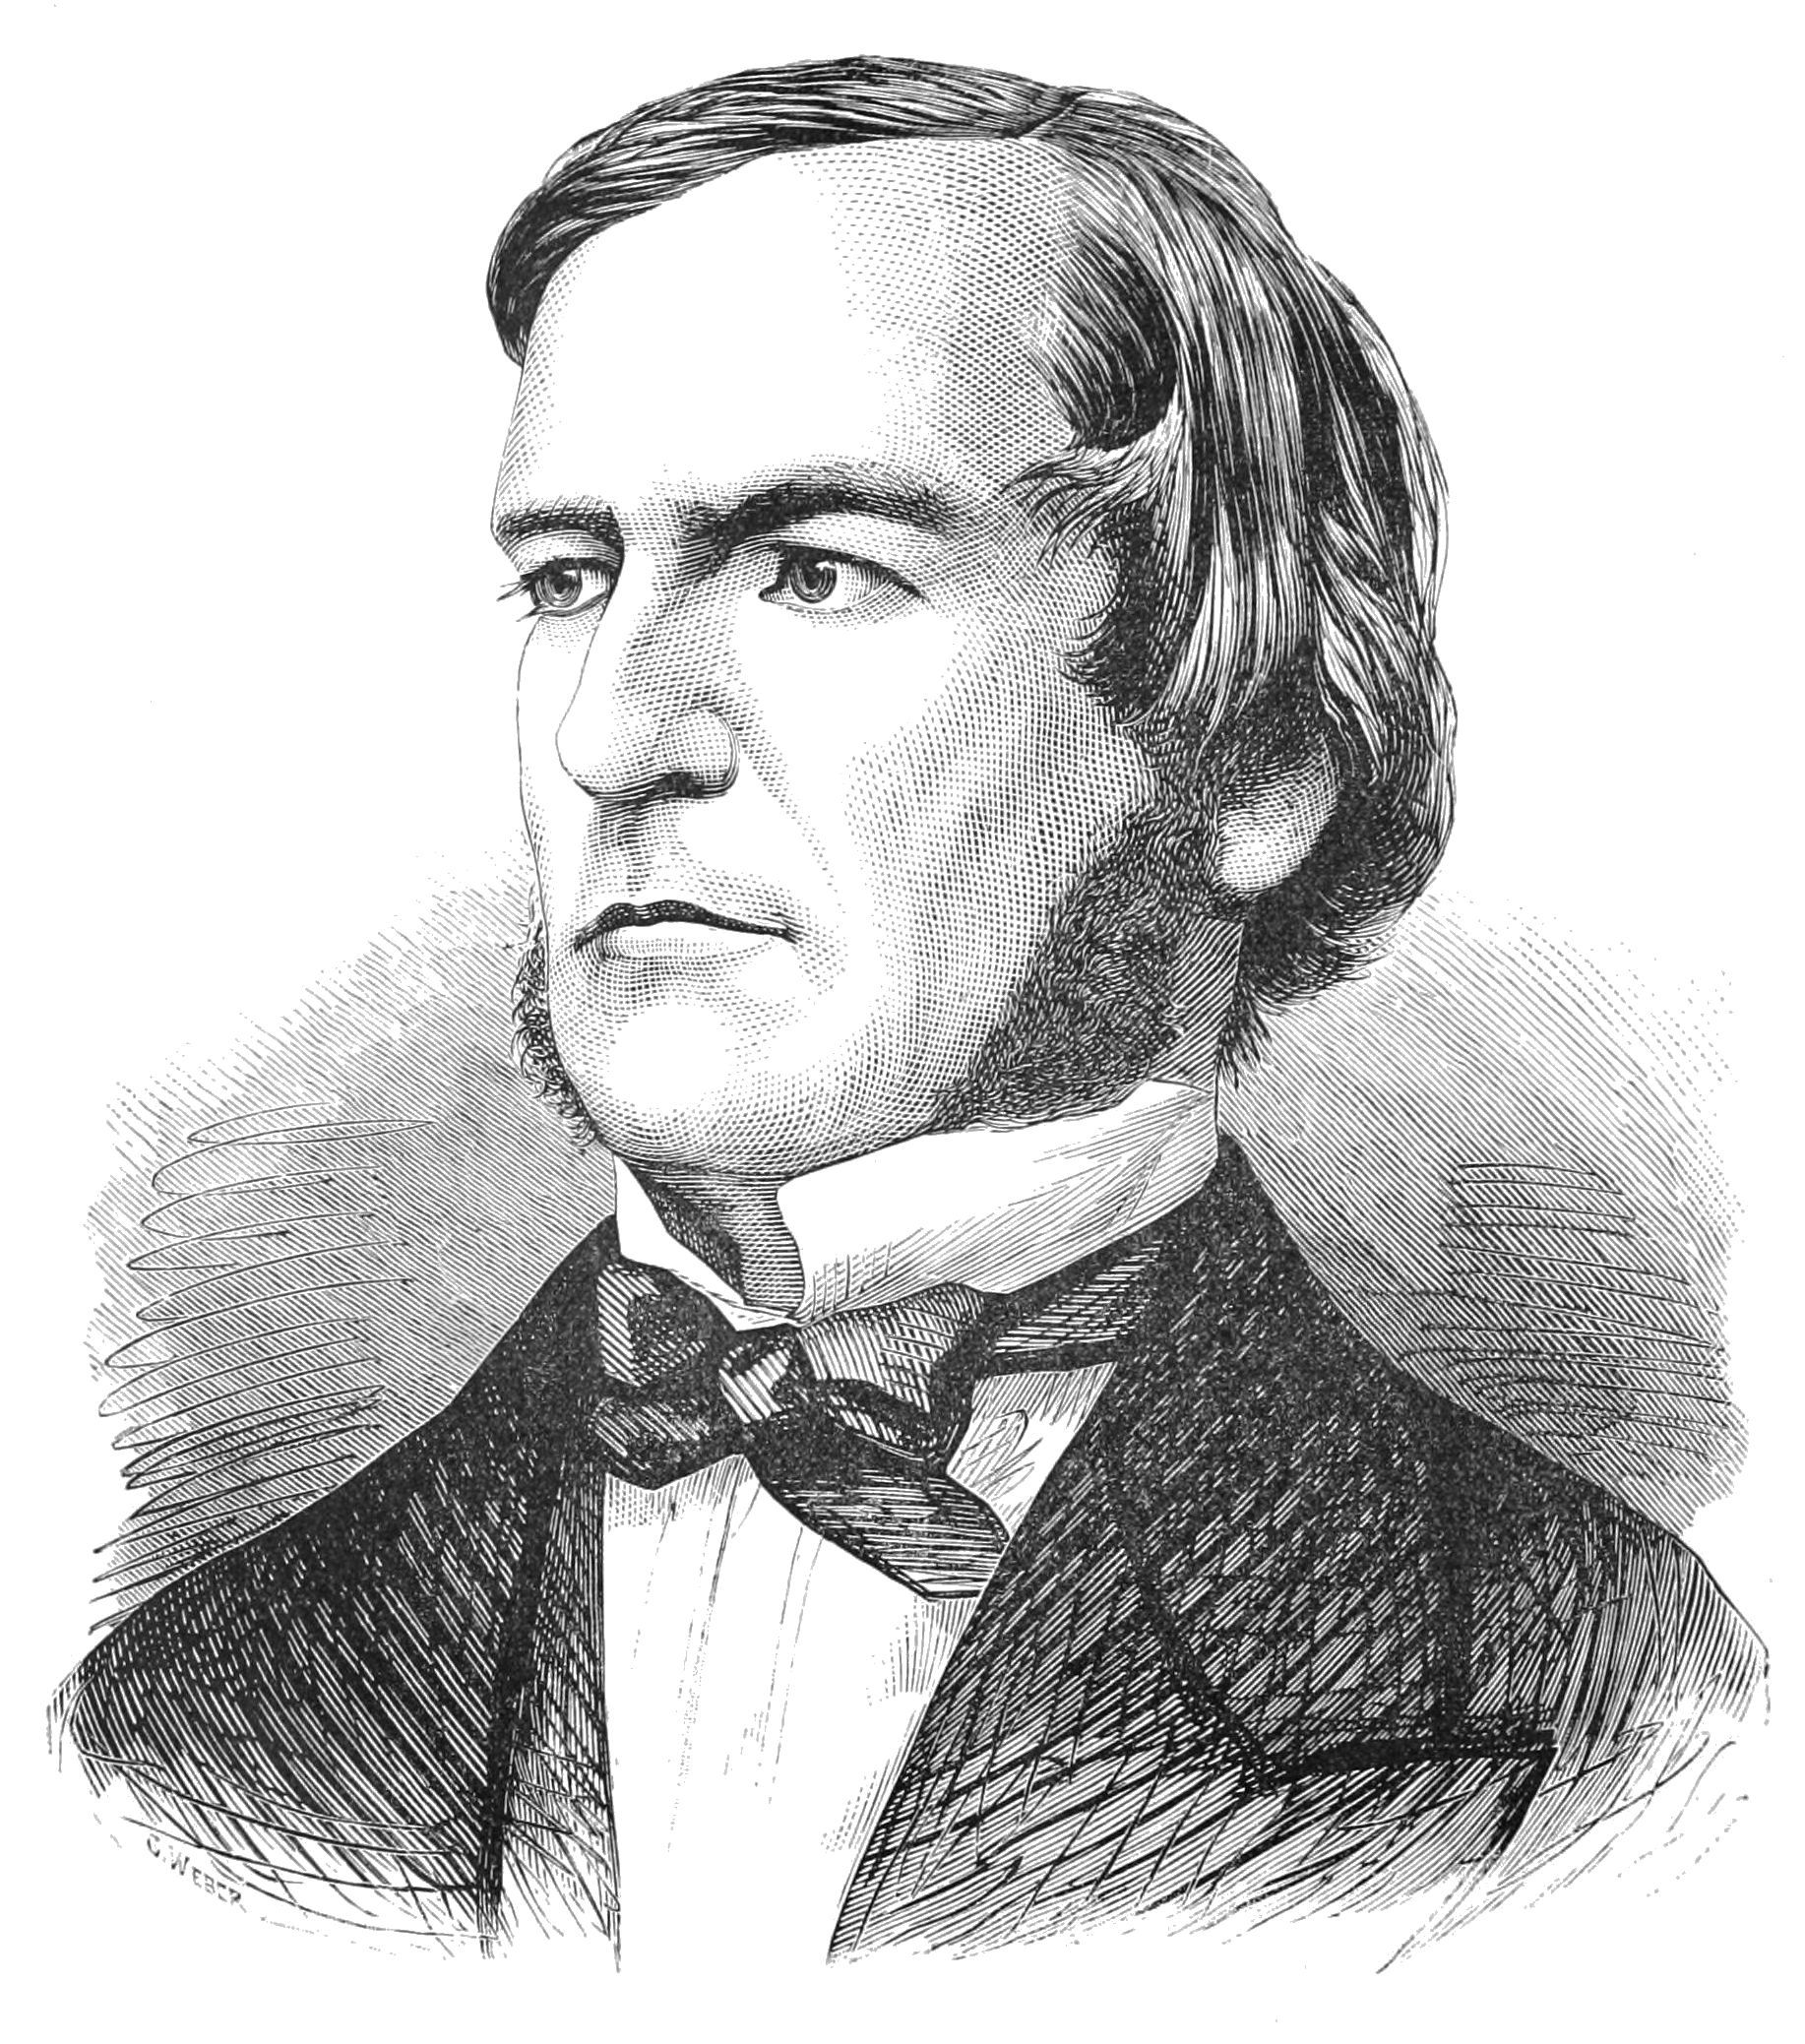
\includegraphics[width=4cm]{boole/img/boole.jpg}
\end{center}
\section{Définition d'une algèbre de Boole}

\begin{definition}[]
    Une \textit{algèbre de Boole}, c'est un ensemble $E$ muni de :
    \begin{itemize}
        \item 	deux lois \textit{binaires} notées + et $\times$;
        \item 	une loi \textit{unaire} qui à $a$ associe $\barmin{a}$;
        \item 	deux éléments particuliers notés 0 et 1;
    \end{itemize}
    et telle que , pour tous éléments a, b et c de E :
    \begin{itemize}
        \item 	Les deux lois binaires sont \textit{commutatives} :
              $a+b=b+a$ et $ab=ba$
        \item 	elles sont aussi associatives :
              $a+(b+c)=(a+b)+c$ et $a(bc)=(ab)c$
        \item 	$\times$ se distribue sur $+$ :
              $a(b+c)=ab+ac$
        \item 	+ se distribue sur $\times$ :
              $\boxed{a+bc=(a+b)(a+c)}$  \\[.5em]
              c'est la seule propriété contre-intuitive, on la notera $(*)$
        \item 	0 est neutre pour $+$: $0+a = a$
        \item 	0 est absorbant pour $\times$ : $0a=0$
        \item 	1 est neutre pour $\times$ : $1a=a$
        \item 	1 est absorbant pour $+$ : $1+a=1$
        \item 	on a $a+\barmin{a}=1$ et $a\barmin{a}=0$
    \end{itemize}
\end{definition}



\begin{exemple}[s]
    \begin{itemize}
        \item 	L'ensemble $\lbrace 0;1\rbrace$ muni de $\vee$, $\wedge$ et $\barmin{\ \ }$ est la plus simple des algèbres de Boole.
        \item 	Si on pose que deux propositions sont égales quand elles sont équivalentes, alors l'ensemble des propositions muni de $\vee$, $\wedge$ et $\barmin{\ \ }$  est une algèbre de Boole,
              0 étant la proposition fausse et 1 la proposition vraie.
        \item 	Comme on le verra au prochain chapitre, lorsqu'on se donne un ensemble $E$ et que l'on considère $\mathcal{P}(E)$, l'ensemble de ses parties, muni des opérations $\cap$ (intersection, joue le rôle de $\times$ ) et $\cup$ (union, joue le rôle de +), alors $P(E)$ est une algèbre de Boole, 0 étant l'\textit{ensemble vide} et 1 étant E lui-même.
    \end{itemize}
\end{exemple}

\begin{exercice}[]
    Montrer que :
    \begin{enumerate}
        \item 	$(a+b)(\barmin{a}+c)(\barmin{b}+\barmin{c})=a\barmin{b}c+\barmin{a}b\barmin{c}$
        \item 	$\barmin{a}\barmin{b}\barmin{c}\barmin{d}+a\barmin{b}\barmin{c}\barmin{d}+	\barmin{a}b\barmin{c}\barmin{d}+ab\barmin{c}\barmin{d}=\barmin{b}\barmin{c}$
        \item 	$ab+\barmin{a}\barmin{b}+ \barmin{a}b=\barmin{a}+b$
    \end{enumerate}
\end{exercice}

\begin{propriete}[s]
    \begin{itemize}
        \item 			Dans une algèbre de Boole, pas besoin de multiplication par un entier car pour tout élément $a$ :
              $$a+a = a$$
              Donc $2a = a$ et par suite pour tout entier naturel non nul $n$ : $na=a$.
        \item Pas besoin de puissances non plus  car pour tout élément $a$ :
              $$aa = a$$
              Donc $a^2 = a$ et par suite pour tout entier naturel non nul $n$ : $a^n=a$.
    \end{itemize}
\end{propriete}

\textbf{Preuve :}\\
Soit $a$ un élément de E:
\begin{multicols}{2}
    \begin{itemize}
        \item 	\begin{tabbing}
                  $a$ \= 	$=a+0$\\[.5em]
                  \>	$=a+a\barmin{a}\qquad$ et on utilise $(*)$\\[.5em]
                  \>	$=(a+a)(a+\barmin{a})$\\[.5em]
                  \>	$=(a+a)1$\\[.5em]
                  \>	$=a+a$
              \end{tabbing}
        \item 	\begin{tabbing}
                  $a$ \= $=a\times 1$\\[.5em]
                  \> $=a(a+\barmin{a})$\\[.5em]
                  \> $=aa+a\barmin{a}$\\[.5em]
                  \> $=aa+0$\\[.5em]
                  \> $=aa$
              \end{tabbing}
    \end{itemize}
\end{multicols}
\begin{propriete}
    Si 2 éléments $x$ et $y$ de E sont tels que $xy=0$ et $x+y=1$, alors $x=\barmin{y}$.
\end{propriete}
\textbf{Preuve :}
\begin{tabbing}
    $x+y=1\quad$	\=	$\Rightarrow\quad (x+y)\barmin{y}=\barmin{y}$\\[.5em]
    \>	$\Rightarrow\quad x\barmin{y}+y\barmin{y}=\barmin{y}$\\[.5em]
    \>	$\Rightarrow\quad x\barmin{y}+0=\barmin{y}$\\[.5em]
    \>	$\Rightarrow\quad x\barmin{y}+xy=\barmin{y}$\\[.5em]
    \>	$\Rightarrow\quad x(\barmin{y}+y)=\barmin{y}$\\[.5em]
    \>	$\Rightarrow\quad x\times 1=\barmin{y}$\\[.5em]
    \>	$\Rightarrow\quad x=\barmin{y}$
\end{tabbing}

\begin{propriete}[ : lois de De Morgan]
    Quels que soient les éléments de $x$ et $y$ de E on a $$\barmin{x\times y}=\barmin{x}+\barmin{y}  \qquad\textrm{et}\qquad \barmin{x+y}=\barmin{x}\times\barmin{y}$$
\end{propriete}

\textbf{Preuve de la première égalité}.\\
Si on pose $A=xy$ et $B=\barmin{x}+\barmin{y}$, alors on doit montrer que $\barmin{A}=B$.\\
On utilise la propriété précédente et on montre donc que $A+B = 1$ et que $AB=0$ :
\begin{multicols}{2}

    \begin{tabbing}
        $B+A$ 	\=	$=\barmin{x}+\barmin{y}+xy$ et on utilise $(*)$\\[.5em]
        \>	$=(\barmin{x}+\barmin{y}+x)(\barmin{x}+\barmin{y}+y)$\\[.5em]
        \>  $=(1+\barmin{y})(1+\barmin{x})$\\[.5em]
        \>  $=1\times 1$\\[.5em]
        \> 	$=1$
    \end{tabbing}

    \begin{tabbing}
        $AB$ \=  $=(\barmin{x}+\barmin{y})xy$\\[.5em]
        \>  $=\barmin{x}xy+\barmin{y}xy$\\[.5em]
        \> 	$=0y+0x$\\[.5em]
        \> 	$=0+0$\\[.5em]
        \> 	$=0$
    \end{tabbing}
\end{multicols}
\begin{exercice}[]
    Montrer la deuxième loi en faisant la même chose.
\end{exercice}



\section{Diagrammes de Karnaugh}

Cette méthode a été développée par Maurice Karnaugh en 1953. Elle fait appel à des tableaux qui représentent des expressions booléennes.\\
On colorie les cases qui correspondent aux différents termes de l'expression. À la fin on peut reconnaître et lire une expression simplifiée.

\begin{propriete}[]
    Un produit correspond à une \textit{intersection}, une somme à une \textit{union}.
\end{propriete}

\subsection{Avec 2 variables}

Le diagramme est un carré dont les quatre cases correspondent aux quatre produits $ab$, $a\barmin{b}$, $\barmin{a}b$, $\barmin{a}\barmin{b}$.

\begin{center}
    \begin{tabular}{|c|c|}
        \hline
        $ab$          & $a\barmin{b}$          \\
        \hline
        $\barmin{a}b$ & $\barmin{a}\barmin{b}$ \\
        \hline
    \end{tabular}
\end{center}
Ci dessous on représente a, b, $\barmin{a}$, $\barmin{b}$ et une dernière expression.
\begin{center}
    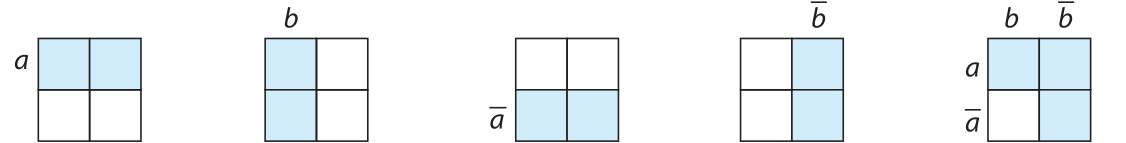
\includegraphics[width=\linewidth]{boole/img/karnaugh1.png}
\end{center}

Cette dernière peut se lire $a+\barmin{b}$ ou bien $ab+a\barmin{b}+\barmin{a}\barmin{b}$.

\begin{exercice}[]
    Propose une troisième interprétation du dernier diagramme.
\end{exercice}

\subsection{Avec 3 variables}

Le diagramme est un rectangle dont les huit cases correspondent aux produits suivants.

\begin{center}
    \begin{tabular}{|c|c|c|c|}

        \hline
        $abc$          & $ab\barmin{c}$          & $a\barmin{b}\barmin{c}$          & $a\barmin{b}c$          \\
        \hline
        $\barmin{a}bc$ & $\barmin{a}b\barmin{c}$ & $\barmin{a}\barmin{b}\barmin{c}$ & $\barmin{a}\barmin{b}c$ \\
        \hline
    \end{tabular}
\end{center}
\begin{center}
    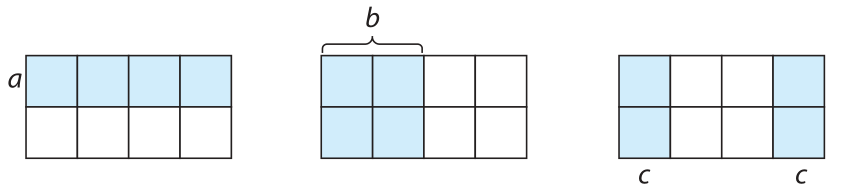
\includegraphics[width=\linewidth]{boole/img/karnaugh2.png}\\

    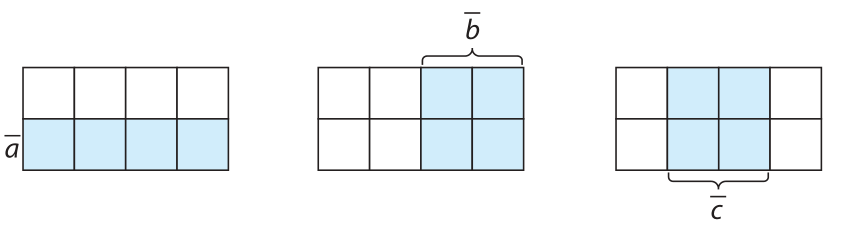
\includegraphics[width=\linewidth]{boole/img/karnaugh3.png}
\end{center}

\begin{exercice}[]
    Faire les tables de Karnaugh des expressions $ab$, $a\barmin{b}$, $ac$, $a\barmin{c}$,  $\barmin{a}b$, $\barmin{a}\barmin{b}$, $\barmin{a}c$, $\barmin{a}\barmin{c}$, $bc$, $\barmin{b}c$, $b\barmin{c}$, $\barmin{b}\barmin{c}$.
\end{exercice}

\section{Exercices}

\begin{exercice}
    $\mathcal{B}$ est une algèbre de Boole.
    \begin{enumerate}
        \item 	Montrer par le calcul que $\forall a\in\mathcal{B},\forall b\in\mathcal{B},\; a+ab = a$;
        \item 	Montrer par le calcul que $\forall a\in\mathcal{B},\forall b\in\mathcal{B},\; a(a+b) = a$.
        \item 	Montrer par le calcul que $\forall a\in\mathcal{B},\forall b\in\mathcal{B},\; a+\barmin{a}b = a+b$.
    \end{enumerate}
    Vérifier ces trois égalités avec des tables de Karnaugh.
\end{exercice}

\begin{exercice}
    \'Ecrire de deux façons possibles l'expression booléenne représentée par le tableau de Karnaugh suivant.
    \begin{center}
        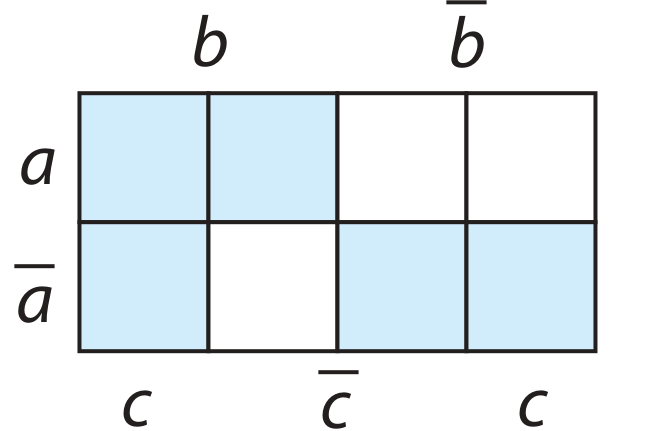
\includegraphics[width=4cm]{boole/img/ex29.png}
    \end{center}
\end{exercice}

\begin{exercice}
    \'Ecrire l'expression booléenne représentée par le tableau de Karnaugh suivant sous la forme d'une somme de deux variables booléennes prises parmi $x$, $y$, $z$, $\barmin{x}
    $, $\barmin{y}$ et $\barmin{z}$.
    \begin{center}
        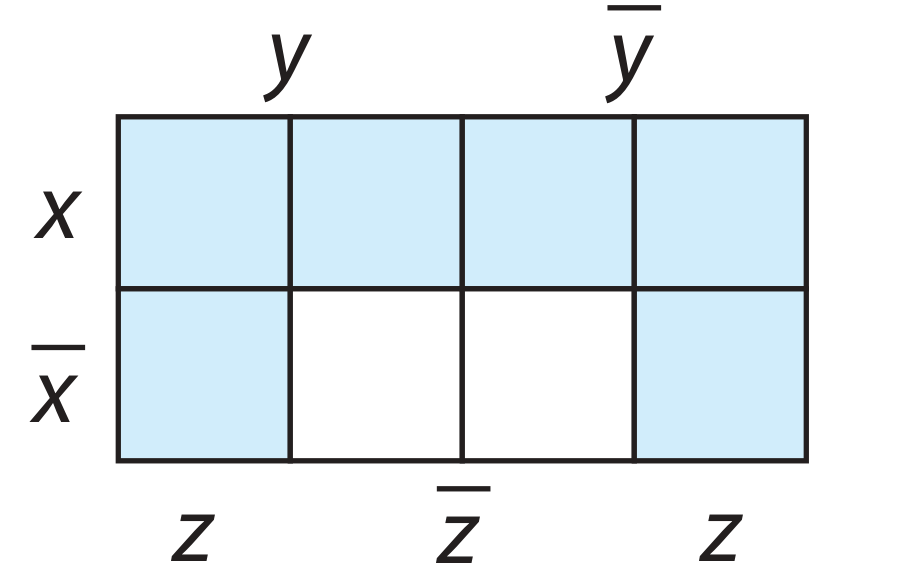
\includegraphics[width=4cm]{boole/img/ex30.png}
    \end{center}
\end{exercice}

\begin{exercice}
    $x$,$y$ et $z$ sont trois élément d'une algèbre booléenne B.\\

    \'Ecrire l'expression $y\overline{(xy+z)}$ sous la forme d'un produit de trois variables booléennes prises parmi $x$, $y$, $z$, $\barmin{x}
    $, $\barmin{y}$ et $\barmin{z}$.\\
\end{exercice}


\begin{exercice}
    $a$,$b$ et $c$ sont trois élément d'une algèbre booléenne B.

    \begin{enumerate}
        \item 	\'Ecrire  l'expression $(a+\barmin{b}c)(b+\barmin{c})$ sous la forme d'une somme de deux produits de deux variables booléennes prises parmi $a$, $b$, $c$, $\barmin{a}
              $, $\barmin{b}$ et $\barmin{c}$.
        \item 	Représenter ce résultat dans une table de Karnaugh et en déduire une nouvelle expression.
    \end{enumerate}
\end{exercice}

\begin{exercice}
    B est une algèbre booléenne. On définit l'opération « nor »{}, notée $\downarrow$ par : $$\forall a\in\mathcal{B},\forall b\in\mathcal{B},\; a\downarrow b = \overline{a+b}$$

    Cette opération est dite \textit{universelle} car elle permet de retrouver toutes les autres opérations.

    \begin{enumerate}
        \item 	Montrer que $\forall a\in\mathcal{B}\; a\downarrow a = \overline{a}$.
        \item 	En déduire que $$\forall a\in\mathcal{B},\forall b\in\mathcal{B},\; (a\downarrow b)\downarrow(a\downarrow b) = a+b$$
        \item 	Comment à partir de $a$, $b$ et $\downarrow$ obtenir $ab$ ?\\
    \end{enumerate}
\end{exercice}

\begin{exercice}[ : Polynésie juin 2018]
    Une société de fabrication et d'installation de fibre optique a besoin de recruter un informaticien, femme ou homme. La direction des ressources humaines considère qu'une candidature est recevable lorsqu'elle satisfait à l'une au moins des conditions suivantes:

    \begin{itemize}
        \item le candidat est âgé de 25 ans ou moins et est titulaire du BTS SIO;
        \item le candidat est âgé de 25 ans ou moins, n'est pas titulaire du BTS SIO et possède de l'expérience;
        \item le candidat est âgé de strictement plus de 25 ans  et est titulaire du BTS SIO;
    \end{itemize}

    \smallskip
    On définit les variables booléennes $a$, $b$, $c$ de la façon suivante:
    \begin{itemize}
        \item $a=1$ si le candidat est âgé de strictement plus de 25 ans, $a=0$ sinon;
        \item $b=1$ si le candidat est titulaire d'un BTS SIO, $b=0$ sinon;
        \item $c=1$ si le candidat a de l'expérience, $c=0$ sinon.
    \end{itemize}

    \begin{enumerate}
        \item Écrire une expression booléenne $E$ traduisant qu'une candidature est recevable, à l'aide des variables booléennes $a$, $b$, $c$.
        \item À l'aide d'un tableau de Karnaugh, déterminer une écriture simplifiée de $E$ sous la forme d'une somme de deux termes. En déduire une interprétation simplifiée des conditions pour qu'une candidature soit recevable.
        \item Une candidate a 21 ans, aucune expérience, mais est titulaire du BTS SIO. Remplit-elle les critères de recrutement?
        \item Donner une expression simple de $\overline{E}$.\\
    \end{enumerate}
\end{exercice}

\begin{exercice}[ : Polynésie mai 2017]

    Cinq joueurs, notés A, B, C, D et E, jouent régulièrement à un jeu en ligne.

    Chaque partie de ce jeu oppose deux adversaires.

    \begin{enumerate}
        \item Dans cette question, on note $J = \lbrace A, B, C, D, E\rbrace$ l'ensemble des cinq joueurs.

              On note $V(x~;~y)$ le prédicat : « le joueur $x$ a déjà battu le joueur $y$ ».

              Ainsi, la valeur $V$(A ; B) est VRAI, et la valeur de $V$(B ; A) est FAUX.

              \smallskip

              On définit trois prédicats :


              \textbf{P1} : $\forall x \in J,\: \exists\, y \in J,\: x \neq y$  et $V(x~;~y)$

              \textbf{P2}: $\exists\, x \in J,\: \forall y \in J,\: x \neq y$  et $V(x~;~y)$

              \textbf{P3}: $\exists\, y \in J,\: \forall x \in J,\: x \neq y$  et $V(x~;~y)$

              \smallskip

              Associer à chaque prédicat P1, P2, P3, celle des trois phrases suivantes qui lui correspond parmi
              les phrases suivantes. Aucune justification n'est demandée.

              « Il existe un joueur qui a été battu par tous les autres joueurs ».

              « Tous les joueurs ont battu au moins un autre joueur  ».

              « Il existe un joueur qui a battu tous les autres joueurs  ».

        \item Un joueur reçoit un bonus lorsqu'il vérifie l'un au moins des trois critères suivants:

              $\bullet~~$ le joueur a participé à 20 parties ou davantage, et il a affronté plusieurs adversaires
              différents ;

              $\bullet~~$  le joueur n'a pas affronté plusieurs adversaires différents, et il a obtenu strictement plus de
              victoires que de défaites ;

              $\bullet~~$  le joueur n'a pas obtenu strictement plus de victoires que de défaites, et il a participé à 20
              parties ou davantage.

              On définit les variables booléennes $a$, $b$, $c$ de la façon suivante:

              $a = 1$ si le joueur a participé à 20 parties ou davantage ; $a = 0$ sinon;

              $b = 1$ si le joueur a affronté plusieurs adversaires différents ; $b = 0$ sinon;

              $c = 1$ si le joueur a obtenu strictement plus de victoires que de défaites ; $c = 0$ sinon.
              \begin{enumalph}
                  \item Écrire une expression booléenne $F$ traduisant les conditions permettant à un joueur d'obtenir le bonus.
                  \item À l'aide d'un tableau de Karnaugh ou d'un calcul booléen, déterminer une écriture simplifiée de $F$ sous forme d'une somme de deux termes.
                  \item En déduire une formulation simplifiée des critères permettant à un joueur d'obtenir le bonus.
              \end{enumalph}
    \end{enumerate}
\end{exercice}


\begin{exercice}[]
    Soient $a$, $b$ et $c$ trois éléments d'une algèbre booléenne $\mathcal{B}$.

    \begin{enumerate}
        \item 	Soient $A=ab+\barmin{c}$ et $B=\barmin{a}+bc$, montrer par le calcul que $$\barmaj{A}=\barmin{a}c+\barmin{b}c$$ et que $$\barmaj{B}=a\barmin{c}+a\barmin{b}$$
        \item 	Soit $C=\barmin{a}\,\barmin{b}\,\barmin{c}+a\barmin{b}c+\barmin{a}\,\barmin{b}+a\barmin{b}\,\barmin{c}$.\\
              Utiliser un diagramme de Karnaugh pour simplifier C.\\
    \end{enumerate}
\end{exercice}

\begin{exercice}[]
    Une salle dédiée à l'informatique va être aménagée au lycée.\\
    Le réseau qui équipera cette salle doit satisfaire au moins l'une des conditions suivantes :

    \begin{itemize}
        \item le réseau compte 5 postes ou plus et il existe un poste qui ne reçoit pas de données en entrée
        \item il existe un poste qui ne reçoit pas de données en entrée, et le réseau compte strictement moins  de 5 postes, et il comporte strictement plus de 12 connexions ;
        \item le réseau comporte 12 connexions ou moins.
    \end{itemize}

    On définit les variables booléennes suivantes:


    \begin{itemize}
        \item $a = 1$ si le réseau compte 5 postes ou plus, $a = 0$ sinon;
        \item $b = 1$ s'il existe un poste qui ne reçoit pas de données en entrée, $b = 0$ sinon;
        \item $c = 1$ si le réseau comporte 12 connexions ou moins, $c = 0$ sinon.
    \end{itemize}

    \begin{enumerate}
        \item Cette question est une question à choix multiple. Une seule réponse est correcte. Recopier sur la copie seulement la réponse correcte. On ne demande pas de justification.

              Parmi les quatre phrases suivantes, donner celle qui traduit la variable $\overline{b}$ :


              \begin{itemize}
                  \item réponse A : « il existe un poste qui reçoit des données en entrée  » ;
                  \item réponse B : « tout poste reçoit des données en entrée  » ;
                  \item réponse C : « il existe un poste qui envoie des données en sortie  » ;
                  \item réponse D : « aucun poste ne reçoit des données en entrée  ».
              \end{itemize}

        \item Donner l'expression booléenne E traduisant les critères voulus pour un réseau informatique.
        \item À l'aide d'un tableau de Karnaugh ou par des calculs, exprimer $E$ comme somme de deux
              variables booléennes.
        \item Traduire les critères de sélection simplifiés, à partir de l'expression obtenue à la question 3.
        \item Un réseau dans lequel 2 postes ne reçoivent pas de données en entrée et qui comporte 15
              connexions répond-il aux critères voulus ? Justifier la réponse.
    \end{enumerate}
\end{exercice}

\begin{exercice}[ : multiplexeur]
    Un multiplexeur est un peu comme une télécommande à 2 boutons : on peut le résumer par une expression booléenne $E$ dépendant de 3 variables $a$, $b$ et $c$.
    \begin{itemize}
        \item Lorsque $a=0$, la valeur de $E$ est celle de $b$.
        \item Lorsque $b=0$, la valeur de $E$ est celle de $c$.
    \end{itemize}
    \begin{enumerate}
        \item À l'aide de cette information, complète la table de vérité suivante.

              \begin{center}
                  \tabstyled
                  \begin{tabular}{|c|c|c|c|}
                      \hline
                      
                      \ccell a & \ccell b & \ccell c & \ccell E \\
                      \hline
                      0      & 0      & 0      &        \\
                      \hline
                      0      & 0      & 1      &        \\
                      \hline
                      0      & 1      & 0      &        \\
                      \hline
                      0      & 1      & 1      &        \\
                      \hline
                      1      & 0      & 0      &        \\
                      \hline
                      1      & 0      & 1      &        \\
                      \hline
                      1      & 1      & 0      &        \\
                      \hline
                      1      & 1      & 1      &        \\
                      \hline
                  \end{tabular}
              \end{center}
        \item Renseigne ensuite la table de Karnaugh
              \begin{center}
                  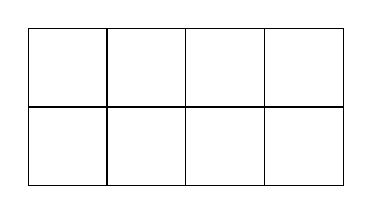
\begin{tikzpicture}
                      \draw (0,0) rectangle (1,1) rectangle(2,0) rectangle(3,1) rectangle(4,0);
                      \draw (0,0) rectangle (1,-1) rectangle(2,0) rectangle(3,-1) rectangle(4,0);
                  \end{tikzpicture}
              \end{center}
        \item Déduis-en une expression simple de $E$.

        \item Dessine le circuit électronique qui représente E.
    \end{enumerate}
\end{exercice}
\chapter{Théorie des ensembles}

\section{Notions de base}

\begin{definition}[: ensemble, éléments]
    Nous nous contenterons de dire qu'un \textit{ensemble} est une \textit{collection d'objets}  appelés \textit{éléments} et qu'on peut clairement dire, lorsqu'on considère un objet, s'il appartient ou non à cet ensemble.\\
    Pour signifier que l'élément $x$ appartient à l'ensemble $E$ on écrit $x\in E$. Pour signifier le contraire on écrit $x\notin E$.
\end{definition}

\begin{exemple}[s]
    \begin{itemize}
        \item
              L'ensemble $\mathcal{J}$ des jours de la semaine peut se noter :
              $$\mathcal{J}=\left\lbrace\ LUN\ ;\ MAR\ ;\ MER\ ;\ JEU\ ;\ VEN\ ;\ SAM\ ;\ DIM\ \right\rbrace$$


        \item 	On note $\N$ l'ensemble de tous les entiers positifs. On a donc $2020\in\N$, mais $3,2\notin\N$.
        \item 	Les solutions dans $\R$ de l'inéquation $x^2<4$ forment un ensemble : $\oio{-2}{2}$.
    \end{itemize}

\end{exemple}
\begin{definition}[s : ensemble vide et singleton]
    \begin{itemize}
        \item 	L'ensemble qui ne contient aucun élément s'appelle \textit{l'ensemble vide} et se note $\emptyset$.
        \item 	Soit $x$ un objet, alors l'ensemble composé de l'unique élément $x$ se note $\lbrace x\rbrace$ et s'appelle un \textit{singleton}.
    \end{itemize}
\end{definition}

\begin{definition}[s : écritures en extension et compréhension]

    Quand un ensemble est \textit{fini} (on reviendra sur cette notion plus tard), on peut donner la liste \textit{exhaustive} de ses éléments comme ceci :\\

    E = $\lbrace $Paris; Marseille; Lyon; Toulouse; Nice; Nantes; Montpellier, Strasbourg, Bordeaux$\rbrace$\\
    L'écriture précédente est appelée \textit{écriture en extension}.\\

    « E est l'ensemble des 9 plus grandes villes de France. » \\
    Lorsqu'on écrit la phrase précédente, on donne une autre manière de définir E : pas par son contenu explicite, mais par une règle que ses éléments vérifient. On parle d'\textit{écriture en compréhension}.
\end{definition}

\begin{exemple}[s]
    \begin{itemize}
        \item 	$E=\lbrace 0;\,1;\;2\rbrace$ est écrit en extension. En compréhension on écrira $E=\lbrace n\in\N,\,n\leq 2\rbrace$.
        \item 	On considère $F=\lbrace n\in\N, n\equiv 2,\,[3]\rbrace$, c'est un ensemble \textit{infini}, on ne peut donc pas écrire la liste de tous ses éléments, mais on peut en donner un « aperçu »  :
              $$F=\left\lbrace 2;\,5;\,8;\,11;\,14;\,...\,\right\rbrace$$
    \end{itemize}
\end{exemple}

\begin{definition}[]
    Quand un ensemble $E$ est \textit{fini}, on appelle \textit{cardinal} de E le nombre de ses éléments, on le note $\card(E)$.
\end{definition}

\begin{remarque}[]
    Un ensemble n'est pas une variable de type \mintinline{python}{list} en \textsc{Python}, ou un tableau de \textsc{Visual Basic}, car il n'y a \textit{a priori} pas d'ordre sur les éléments de l'ensemble.\\
    Ainsi l'ensemble $\lbrace \text{ crayon ; stylo }\rbrace$ est le même que l'ensemble $\lbrace \text{ stylo ; crayon }\rbrace$.\\
    En revanche en \textsc{Python}, on a \mintinline{python}{['stylo', 'crayon']} et \mintinline{python}{['crayon', 'stylo']} sont deux listes différentes.


\end{remarque}

\begin{definition}[ : inclusion]
    Soit $A$ et $B$ deux ensembles. Si tout élément de $A$ est également un élément de $B$ alors on dit que \textit{$A$ est inclus dans $B$}.\\
    On écrit alors $A\subset B$ et cela revient à écrire : $\forall x\in A,\,x\in B$.
\end{definition}

\begin{exemple}[s]
    \begin{itemize}
        \item 	En reprenant un exemple précédent on a :
              $$\lbrace \text{ LUN ; JEU ; VEN }\rbrace \subset \mathcal{J}$$
        \item 	Notons $A$ l'ensemble des élèves de la classe et $B$ l'ensemble des élèves de la classe qui habitent Saint-Brieuc.\\
              \begin{center}
                  \begin{tikzpicture}
                      \draw[fill = UGLiBlue,opacity = .3](0,0) ellipse (2 and 4/3);
                      \draw[fill = UGLiPurple,opacity = .3](.5,0) ellipse (1 and 2/3);
                      \draw (-1,0) node{$A$};
                      \draw (1,0) node{ $B$};
                  \end{tikzpicture}

                  $B\subset A$
              \end{center}
    \end{itemize}
\end{exemple}
\begin{remarque}[s]
    \begin{itemize}
        \item Quel que soit l'ensemble $E$, on a $E\subset E$ car la proposition $\forall x\in E,\,x\in E$ est vraie.
        \item 	Quel que soit l'ensemble $A$, $\emptyset \subset A$ : en effet la proposition suivante est vraie : $\forall x\in\emptyset,\,x\in A$.\\
              Cela peut paraître abusif étant donné qu'il n'y a aucun élément dans $\emptyset$. Faisons alors appel à nos cours de logique et montrons que la proposition contraire est fausse, ce qui revient au même. Cette proposition contraire s'énonce :\\
              $\exists\, x\in\emptyset,\,x\notin A$. Elle est évidemment fausse puisqu'on ne peut trouver $x\in\emptyset$.
        \item 	Il n'existe pas d'\textit{ensemble de tous les ensembles} : on ne peut pas se dire que les ensembles peuvent tous être rangés dans un « gros ensemble » . En revanche (et c'est ce qu'on va faire), il est possible de se donner un ensemble de départ $E$ et de considérer tous les ensembles inclus dedans.
    \end{itemize}
\end{remarque}
\section{L'algèbre de Boole des parties d'un ensemble}
\begin{definition}[ : ensemble des parties d'un ensemble]
    On se donne un ensemble $E$. L'ensemble de \textit{tous les ensembles inclus dans } $E$ se note $\mathcal{P}(E)$. On l'appelle aussi \textit{ensemble des parties de $E$}.
    \begin{itemize}
        \item 	On a vu que $\emptyset\subset E$, ce qui se réécrit $\emptyset\in\mathcal{P}(E)$.
        \item 	De même $E\subset E$, ce qui se réécrit $E\in\mathcal{P}(E)$.
    \end{itemize}
\end{definition}
\begin{exemple}[]
    Posons $E=\lbrace a;\,b;\,c\rbrace$ et donnons tous les éléments de $\mathcal{P}(E)$ :
    \begin{itemize}
        \item 	il y a $\emptyset$;
        \item 	il y a $\lbrace a\rbrace$, $\lbrace b\rbrace$ et $\lbrace c\rbrace$;
        \item 	il y a $\lbrace a;\,b\rbrace$, $\lbrace a;\,c\rbrace$ et $\lbrace b;\,c\rbrace$, parties à 2 éléments.
        \item 	il y a $E$ lui même.
    \end{itemize}
    Ainsi $\mathcal{P}(E)=\left\lbrace \emptyset;\,\lbrace a\rbrace ;\,\lbrace b\rbrace ;\,\lbrace c\rbrace ;\,\lbrace a;\,b\rbrace ;\,\lbrace a;\,c\rbrace ;\,\lbrace b;\,c\rbrace ;\,\lbrace a;\,b;\,c\rbrace \right\rbrace$ comporte 8 éléments.
\end{exemple}

\begin{exercice}[]
    Déterminer $\mathcal{P}(E)$ lorsque $E=\lbrace r;\,s;\,t;\,u;\,v\rbrace$.
\end{exercice}
\begin{definition}[ : intersection]
    \begin{center}
        \begin{tikzpicture}
            \draw[fill = UGLiBlue,opacity = .2](0,0) ellipse (2 and 4/3);
            \draw[fill = UGLiPurple,opacity = .2](2,0) ellipse (2 and 4/3);
            \draw (-1,0) node{$A$};
            \draw (3,0) node{$B$};
            \draw (1,0) node{$A\cap B$};
        \end{tikzpicture}
    \end{center}
    Soient $A$ et $B$ deux ensembles. On appelle \textit{intersection} de $A$ et de $B$ et on note $A\cap B$ l'ensemble dont les éléments appartiennent à la
    fois à $A$ et à $B$.
\end{definition}

\begin{definition}[ : union]
    Soient $A$ et $B$ deux ensembles. On appelle \textit{union} de $A$ et de $B$ et on note $A\cup B$ l'ensemble dont les éléments à $A$ ou bien à $B$.\\
    \begin{center}
        \begin{tikzpicture}
            \begin{scope}
                \draw[fill = UGLiBlue!30](0,0) ellipse (2 and 4/3);
                \draw[fill = UGLiBlue!30](2,0) ellipse (2 and 4/3);
                \clip	ellipse (2 and 4/3);
                \draw[fill = UGLiBlue!30, UGLiBlue!30](2,0) ellipse (2 and 4/3);
                \draw[dashed](2,0) ellipse (2 and 4/3);
                \clip (2,0) ellipse (2 and 4/3);
                \draw[fill = UGLiBlue!30, UGLiBlue!30] ellipse (2 and 4/3);
                \draw[dashed] ellipse (2 and 4/3);
            \end{scope}
            \draw (3,0) node{$B$};
            \draw (-1,0) node{$A$};
            \draw (1,-1.6) node{$A\cup B$};
        \end{tikzpicture}
    \end{center}
\end{definition}

\begin{exemple}
    Considérons les ensembles $A=\lbrace \ u\ ;\ v\ ;\ w\ \rbrace$ et $B=\lbrace \ u\ ;\ w\ ;\ x\ ;\ y\ \rbrace$.\\
    Alors \textbf{ $$A\cap B=\lbrace \ u\ ;\ w\ \rbrace$$} et \textbf{ $$A\cup B=\lbrace \ u\ ;\ v\ ;\ w\ ;\ x\ ;\ y\ \rbrace$$}
\end{exemple}
\begin{definition}[ : complémentaire]
    Soit $A$ une partie de E.\\
    On appelle complémentaire de $A$  dans $E$ et on note $\overline{A}$ l'ensemble des éléments de $E$ qui n'appartiennent pas à $A$.
    \begin{center}
        \begin{tikzpicture}
            \draw[fill = UGLiBlue!30](0,0) ellipse (2 and 4/3);
            \draw[fill = white](1,0) ellipse (.9 and 2/3);
            \draw (1,0) node{$A$};
            \draw (-1,0) node{$\overline{A}$};
            \draw (2,0)--(3,0) node[right]{$E$};
        \end{tikzpicture}
    \end{center}
\end{definition}

\begin{exemple}[]
    En prenant $E=\left\lbrace\ LUN\ ;\ MAR\ ;\ MER\ ;\ JEU\ ;\ VEN\ ;\ SAM\ ;\ DIM\ \right\rbrace$ comme ensemble de départ, le complémentaire dans $E$ de $\lbrace  LUN;\, JEU;\, VEN\rbrace$ est $\lbrace  MAR;\, MER;\, SAM;\,DIM\rbrace$.
\end{exemple}
\begin{exercice}[]
    $A$ et $B$ sont deux parties de $E$. Colorier l'ensemble demandé.
    \begin{multicols}{3}
        \begin{enumerate}
            \item 	$A\cup \overline{B}$\\

                  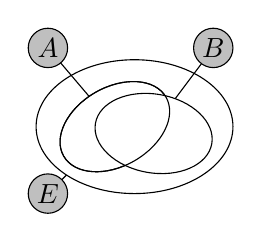
\begin{tikzpicture}[scale=.5]
                      \draw (-1.7,-1.7) -- (0,0);
                      \draw [fill = gray!50](-1.7,-1.7) circle(.5) node{$E$};
                      \draw [fill = white](0.5,0) ellipse (2.5 and 1.7);

                      \draw (-1.7,2) -- (0,0);
                      \draw [fill = gray!50](-1.7,2) circle(.5) node{$A$};
                      \draw [rotate=30,fill = white](0,0) ellipse (1.5 and 1);

                      \draw (2.5,2) -- (1,0);
                      \draw [fill = gray!50](2.5,2) circle(.5) node{$B$};
                      \draw [rotate=-10, fill = white](1,0) ellipse (1.5 and 1);

                      \draw [rotate=30](0,0) ellipse (1.5 and 1);
                  \end{tikzpicture}

            \item 	$A\cap \overline{B}$\\

                  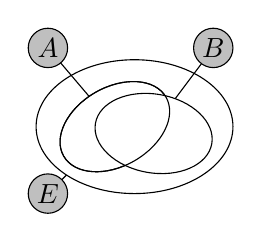
\begin{tikzpicture}[scale=.5]
                      \draw (-1.7,-1.7) -- (0,0);
                      \draw [fill = gray!50](-1.7,-1.7) circle(.5) node{$E$};
                      \draw [fill = white](0.5,0) ellipse (2.5 and 1.7);

                      \draw (-1.7,2) -- (0,0);
                      \draw [fill = gray!50](-1.7,2) circle(.5) node{$A$};
                      \draw [rotate=30,fill = white](0,0) ellipse (1.5 and 1);

                      \draw (2.5,2) -- (1,0);
                      \draw [fill = gray!50](2.5,2) circle(.5) node{$B$};
                      \draw [rotate=-10, fill = white](1,0) ellipse (1.5 and 1);

                      \draw [rotate=30](0,0) ellipse (1.5 and 1);
                  \end{tikzpicture}
            \item 	$\overline{A\cap B}$\\

                  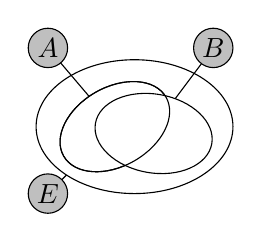
\begin{tikzpicture}[scale=.5]
                      \draw (-1.7,-1.7) -- (0,0);
                      \draw [fill = gray!50](-1.7,-1.7) circle(.5) node{$E$};
                      \draw [fill = white](0.5,0) ellipse (2.5 and 1.7);

                      \draw (-1.7,2) -- (0,0);
                      \draw [fill = gray!50](-1.7,2) circle(.5) node{$A$};
                      \draw [rotate=30,fill = white](0,0) ellipse (1.5 and 1);

                      \draw (2.5,2) -- (1,0);
                      \draw [fill = gray!50](2.5,2) circle(.5) node{$B$};
                      \draw [rotate=-10, fill = white](1,0) ellipse (1.5 and 1);

                      \draw [rotate=30](0,0) ellipse (1.5 and 1);
                  \end{tikzpicture}
            \item 	$\overline{A\cup B}$\\

                  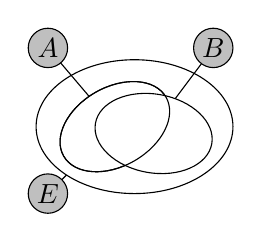
\begin{tikzpicture}[scale=.5]
                      \draw (-1.7,-1.7) -- (0,0);
                      \draw [fill = gray!50](-1.7,-1.7) circle(.5) node{$E$};
                      \draw [fill = white](0.5,0) ellipse (2.5 and 1.7);

                      \draw (-1.7,2) -- (0,0);
                      \draw [fill = gray!50](-1.7,2) circle(.5) node{$A$};
                      \draw [rotate=30,fill = white](0,0) ellipse (1.5 and 1);

                      \draw (2.5,2) -- (1,0);
                      \draw [fill = gray!50](2.5,2) circle(.5) node{$B$};
                      \draw [rotate=-10, fill = white](1,0) ellipse (1.5 and 1);

                      \draw [rotate=30](0,0) ellipse (1.5 and 1);
                  \end{tikzpicture}

            \item 	$\overline{A}\cap \overline{B}$\\

                  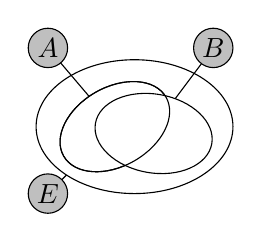
\begin{tikzpicture}[scale=.5]
                      \draw (-1.7,-1.7) -- (0,0);
                      \draw [fill = gray!50](-1.7,-1.7) circle(.5) node{$E$};
                      \draw [fill = white](0.5,0) ellipse (2.5 and 1.7);

                      \draw (-1.7,2) -- (0,0);
                      \draw [fill = gray!50](-1.7,2) circle(.5) node{$A$};
                      \draw [rotate=30,fill = white](0,0) ellipse (1.5 and 1);

                      \draw (2.5,2) -- (1,0);
                      \draw [fill = gray!50](2.5,2) circle(.5) node{$B$};
                      \draw [rotate=-10, fill = white](1,0) ellipse (1.5 and 1);

                      \draw [rotate=30](0,0) ellipse (1.5 and 1);
                  \end{tikzpicture}

            \item 	$\overline{A}\cup\overline{B}$\\

                  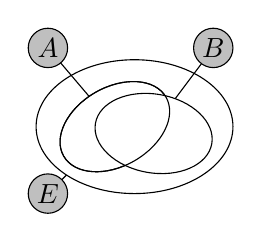
\begin{tikzpicture}[scale=.5]
                      \draw (-1.7,-1.7) -- (0,0);
                      \draw [fill = gray!50](-1.7,-1.7) circle(.5) node{$E$};
                      \draw [fill = white](0.5,0) ellipse (2.5 and 1.7);

                      \draw (-1.7,2) -- (0,0);
                      \draw [fill = gray!50](-1.7,2) circle(.5) node{$A$};
                      \draw [rotate=30,fill = white](0,0) ellipse (1.5 and 1);

                      \draw (2.5,2) -- (1,0);
                      \draw [fill = gray!50](2.5,2) circle(.5) node{$B$};
                      \draw [rotate=-10, fill = white](1,0) ellipse (1.5 and 1);

                      \draw [rotate=30](0,0) ellipse (1.5 and 1);
                  \end{tikzpicture}



            \item 	$\overline{A\cap \overline{B}}$\\

                  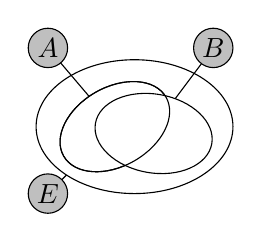
\begin{tikzpicture}[scale=.5]
                      \draw (-1.7,-1.7) -- (0,0);
                      \draw [fill = gray!50](-1.7,-1.7) circle(.5) node{$E$};
                      \draw [fill = white](0.5,0) ellipse (2.5 and 1.7);

                      \draw (-1.7,2) -- (0,0);
                      \draw [fill = gray!50](-1.7,2) circle(.5) node{$A$};
                      \draw [rotate=30,fill = white](0,0) ellipse (1.5 and 1);

                      \draw (2.5,2) -- (1,0);
                      \draw [fill = gray!50](2.5,2) circle(.5) node{$B$};
                      \draw [rotate=-10, fill = white](1,0) ellipse (1.5 and 1);

                      \draw [rotate=30](0,0) ellipse (1.5 and 1);
                  \end{tikzpicture}

            \item 	$(A\cap\overline{B})\cup(A\cap B)$\\

                  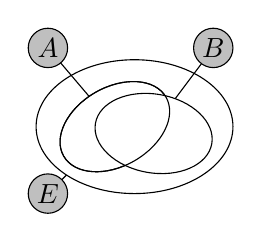
\begin{tikzpicture}[scale=.5]
                      \draw (-1.7,-1.7) -- (0,0);
                      \draw [fill = gray!50](-1.7,-1.7) circle(.5) node{$E$};
                      \draw [fill = white](0.5,0) ellipse (2.5 and 1.7);

                      \draw (-1.7,2) -- (0,0);
                      \draw [fill = gray!50](-1.7,2) circle(.5) node{$A$};
                      \draw [rotate=30,fill = white](0,0) ellipse (1.5 and 1);

                      \draw (2.5,2) -- (1,0);
                      \draw [fill = gray!50](2.5,2) circle(.5) node{$B$};
                      \draw [rotate=-10, fill = white](1,0) ellipse (1.5 and 1);

                      \draw [rotate=30](0,0) ellipse (1.5 and 1);
                  \end{tikzpicture}

            \item 	$(A\cap\overline{B})\cup(\overline{A}\cap{B})$\\

                  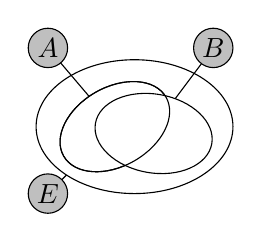
\begin{tikzpicture}[scale=.5]
                      \draw (-1.7,-1.7) -- (0,0);
                      \draw [fill = gray!50](-1.7,-1.7) circle(.5) node{$E$};
                      \draw [fill = white](0.5,0) ellipse (2.5 and 1.7);

                      \draw (-1.7,2) -- (0,0);
                      \draw [fill = gray!50](-1.7,2) circle(.5) node{$A$};
                      \draw [rotate=30,fill = white](0,0) ellipse (1.5 and 1);

                      \draw (2.5,2) -- (1,0);
                      \draw [fill = gray!50](2.5,2) circle(.5) node{$B$};
                      \draw [rotate=-10, fill = white](1,0) ellipse (1.5 and 1);

                      \draw [rotate=30](0,0) ellipse (1.5 and 1);
                  \end{tikzpicture}
        \end{enumerate}
    \end{multicols}
\end{exercice}
\begin{remarque}[]
    Quand on considère 2 parties d'un ensemble E, leur union en est encore une, de même que leur intersection. Il en va encore de même pour le complémentaire d'une partie de E. Ces trois opérations sont donc « internes »  à $\mathcal{P}(E)$, et on peut même énoncer le résultat suivant :
\end{remarque}

\begin{propriete}[]
    Soit $E$ un ensemble. Alors lorsqu'on munit $\mathcal{P}(E)$ de $\cup$, $\cap$ et de l'opération « complémentaire » , on obtient une \textit{algèbre de Boole} :\begin{itemize}
        \item 	0 se note $\emptyset$;
        \item 	1 se note $E$;
        \item 	+ se note $\cup$;
        \item 	$\times$ se note $\cap$.
    \end{itemize}
\end{propriete}
Cela implique qu'on peut effectuer les calculs dans $\mathcal{P}(E)$ de la même manière qu'on effectue les calculs booléens.
\begin{exemple}[]
    \begin{tabbing}
        $A\cup(B\cap \barmaj{A})$ \= $=(A\cup B)\cap(A\cup \barmaj{A})\qquad$ \=car $\cup$ se distribue sur $\cap$\\
        \> $= (A\cup B)\cap E$ \>puisque $A\cup \barmaj{A}=E$ (tout comme $a+\barmin{a}=1$)\\
        \> $= A\cup B$ \> car $E$ est neutre pour $\cap$ \\
        \> \>(tout comme $1$ est neutre pour $\times$)
    \end{tabbing}
\end{exemple}

On peut aussi utiliser des \textit{diagrammes de Venn} (les dessins « à base de patatoïdes »  vus plus haut) dans les cas simples.

\begin{exercice}[]
    Illustrer à l'aide d'un diagramme  que l'égalité $A\cap B = A\cap C$ n'entraîne pas automatiquement $B=C$.
\end{exercice}

\begin{propriete}[ : lois de De Morgan]
    Pour toutes parties $A$ et $B$ de $E$ on a
    $$\barmaj{A\cup B}=\barmaj{A}\cap\barmaj{B}\qquad\text{et}\qquad\barmaj{A\cap B}=\barmaj{A}\cup\barmaj{B}$$
    puisque  $\mathcal{P}(E)$  est une algèbre de Boole.
\end{propriete}
\begin{methode}[]
    Soient $A$ et $B$ deux parties de E, comment écrire l'ensemble $$F=\lbrace \,x\in E,\,x\in A\:et\:x\notin B\cup C\rbrace$$
    à l'aide d'union, intersection et complémentaire ?\\

    \begin{itemize}
        \item 	les « et »  représentent des $\cap$;
        \item 	les « ou »  représentent de $\cup$;
        \item 	pour tout ensemble $G$, $x\notin G$ équivaut à $x\in\barmaj{G}$.
    \end{itemize}

    Donc dans ce cas
    \begin{tabbing}
        $F$ \= $=A\cap\overline{B\cup C}\qquad$ et on utilise une loi de De Morgan\\
        \> $=A\cap \barmaj{B}\cap \barmaj{C}$
    \end{tabbing}
\end{methode}

\begin{exercice}[]
    Dans $\mathcal{P}(E)$ on définit l'opération $\Delta$ comme ceci :
    $$A\,\Delta\,B=\lbrace x\in E,\, x\in A\cup B\:et\:x\notin{A\cap B}\rbrace$$
    \begin{enumerate}
        \item 	Faire un diagramme de Venn et colorier $A\,\Delta\,B$.
        \item 	À quelle opération logique $\Delta$ correspond-elle ?
        \item 	Exprimer $\Delta$ à l'aide de $\cup$, $\cap$ et le complémentaire.
        \item 	Montrer par le calcul que $(A\,\Delta\,B)\,\Delta\,C =A\,\Delta\,(B\,\Delta\,C)$.
    \end{enumerate}
\end{exercice}

\begin{exercice}[]
    Dans $\mathcal{P}(E)$ on définit l'opération $\backslash$ comme ceci :
    $$A\backslash B=\lbrace x\in E,\, x\in A\:et\:x\notin B\rbrace$$
    \begin{enumerate}
        \item 	Faire un diagramme de Venn et colorier $A\backslash B$.
        \item 	Exprimer $\backslash$ à l'aide de $\cup$, $\cap$ et le complémentaire.
        \item 	Montrer par le calcul que $A\backslash (B\cap C)=(A\backslash B)\cup(A\backslash C)$.
    \end{enumerate}
\end{exercice}




\section{Produit cartésien}

\begin{definition}[ : produit cartésien de deux ensembles]
    Soient $E$ et $F$ deux ensembles, on appelle \textit{produit cartésien} de $E$ par $F$ et on note $E\times F$ l'ensemble des couples $(x;\,y)$, où $x\in E$ et $y\in F$.
    $$E\times F = \left\lbrace  (x;\,y),\:x\in E,\,y\in F\right\rbrace$$
\end{definition}

\begin{exemple}[s]
    \begin{itemize}
        \item 	Prenons $E=\left\lbrace bille;\,ballon\right\rbrace$ et $F=\left\lbrace rouge;\,vert;\,bleu\right\rbrace$ alors on peut représenter $E\times F$ de la manière suivante :

              \begin{center}
                  \tabstyle[UGLiBlue]
                  \begin{tabular}{|c|c|c|}
                      \hline\rowcolor{UGLiBlue}
                      \cellcolor{white}              & \ccell bille     & \ccell ballon     \\
                      \hline
                      \cellcolor{UGLiBlue}\ccell rouge & (bille; rouge) & (ballon; rouge) \\
                      \hline
                      \cellcolor{UGLiBlue}\ccell vert  & (bille; vert)  & (ballon; vert)  \\
                      \hline
                      \cellcolor{UGLiBlue}\ccell bleu  & (bille; bleu)  & (ballon; bleu)  \\
                      \hline
                  \end{tabular}
              \end{center}

        \item 	$\R\times\R$ se note aussi $\R^2$. Quand on s'est donné un repère du plan $\repaff$, alors tout point du plan possède un unique couple de coordonnées dans $\R^2$ et réciproquement, à tout couple de $\R^2$ correspond un unique point du plan. C'est pourquoi on identifie $\R^2$ au plan... et $R^3$ à l'espace.
        \item 	Le produit cartésien est fondamental dans le domaine des bases de données.
    \end{itemize}\end{exemple}

\begin{exercice}[]
    En prenant $E=\lbrace 1;\,2\rbrace$ et $F=\lbrace a;\,b;\,c\rbrace$ construire $E\times F$ et $F\times E$ et montrer que ces ensembles sont différents.
\end{exercice}

\begin{propriete}[]
    Si $\card(E)=n$ et $\card(F)=p$ alors $\card(E\times F)=n\times p$.
\end{propriete}

\begin{definition}[: produit cartésien de plusieurs ensembles]
    Soient $E_1$, \ldots $E_n$ $k$ ensembles ($n$ entier supérieur à 2), on note
    $$\prod_{k=1}^{k=n}E_k=E_1\times\ldots\times E_n$$
    l'ensemble des \textit{n-uplets} $(x_1;\,\ldots;\,x_n)$ ou chaque $x_k$ appartient à $E_k$.\\ On dit que c'est le \textit{produit cartésien} des ensembles $E_k$.
\end{definition}

\begin{propriete}[]
    Quand tous les ensembles sont finis, le cardinal de l'ensemble produit s'obtient en multipliant les cardinaux des ensembles.
\end{propriete}
\section{Relations binaires}
\begin{definition}[ : relation binaire]
    Soient $E$ et $F$ deux ensembles. Une \textit{relation binaire de $E$ vers $F$} c'est la donnée de certains \textit{couples} $(x_i;\,y_i)$; où $x_i\in E$ et $y_i\in F$.\\
    $E$ est appelé \textit{ensemble de départ} et $F$ \textit{ensemble d'arrivée}.
    L'ensemble de ces couples (notons-le $G$), est appelé le \textit{graphe} de la relation. C'est une partie de $E\times F$.
\end{definition}

\begin{exemple}[ : avec un diagramme sagittal]
    \begin{center}
        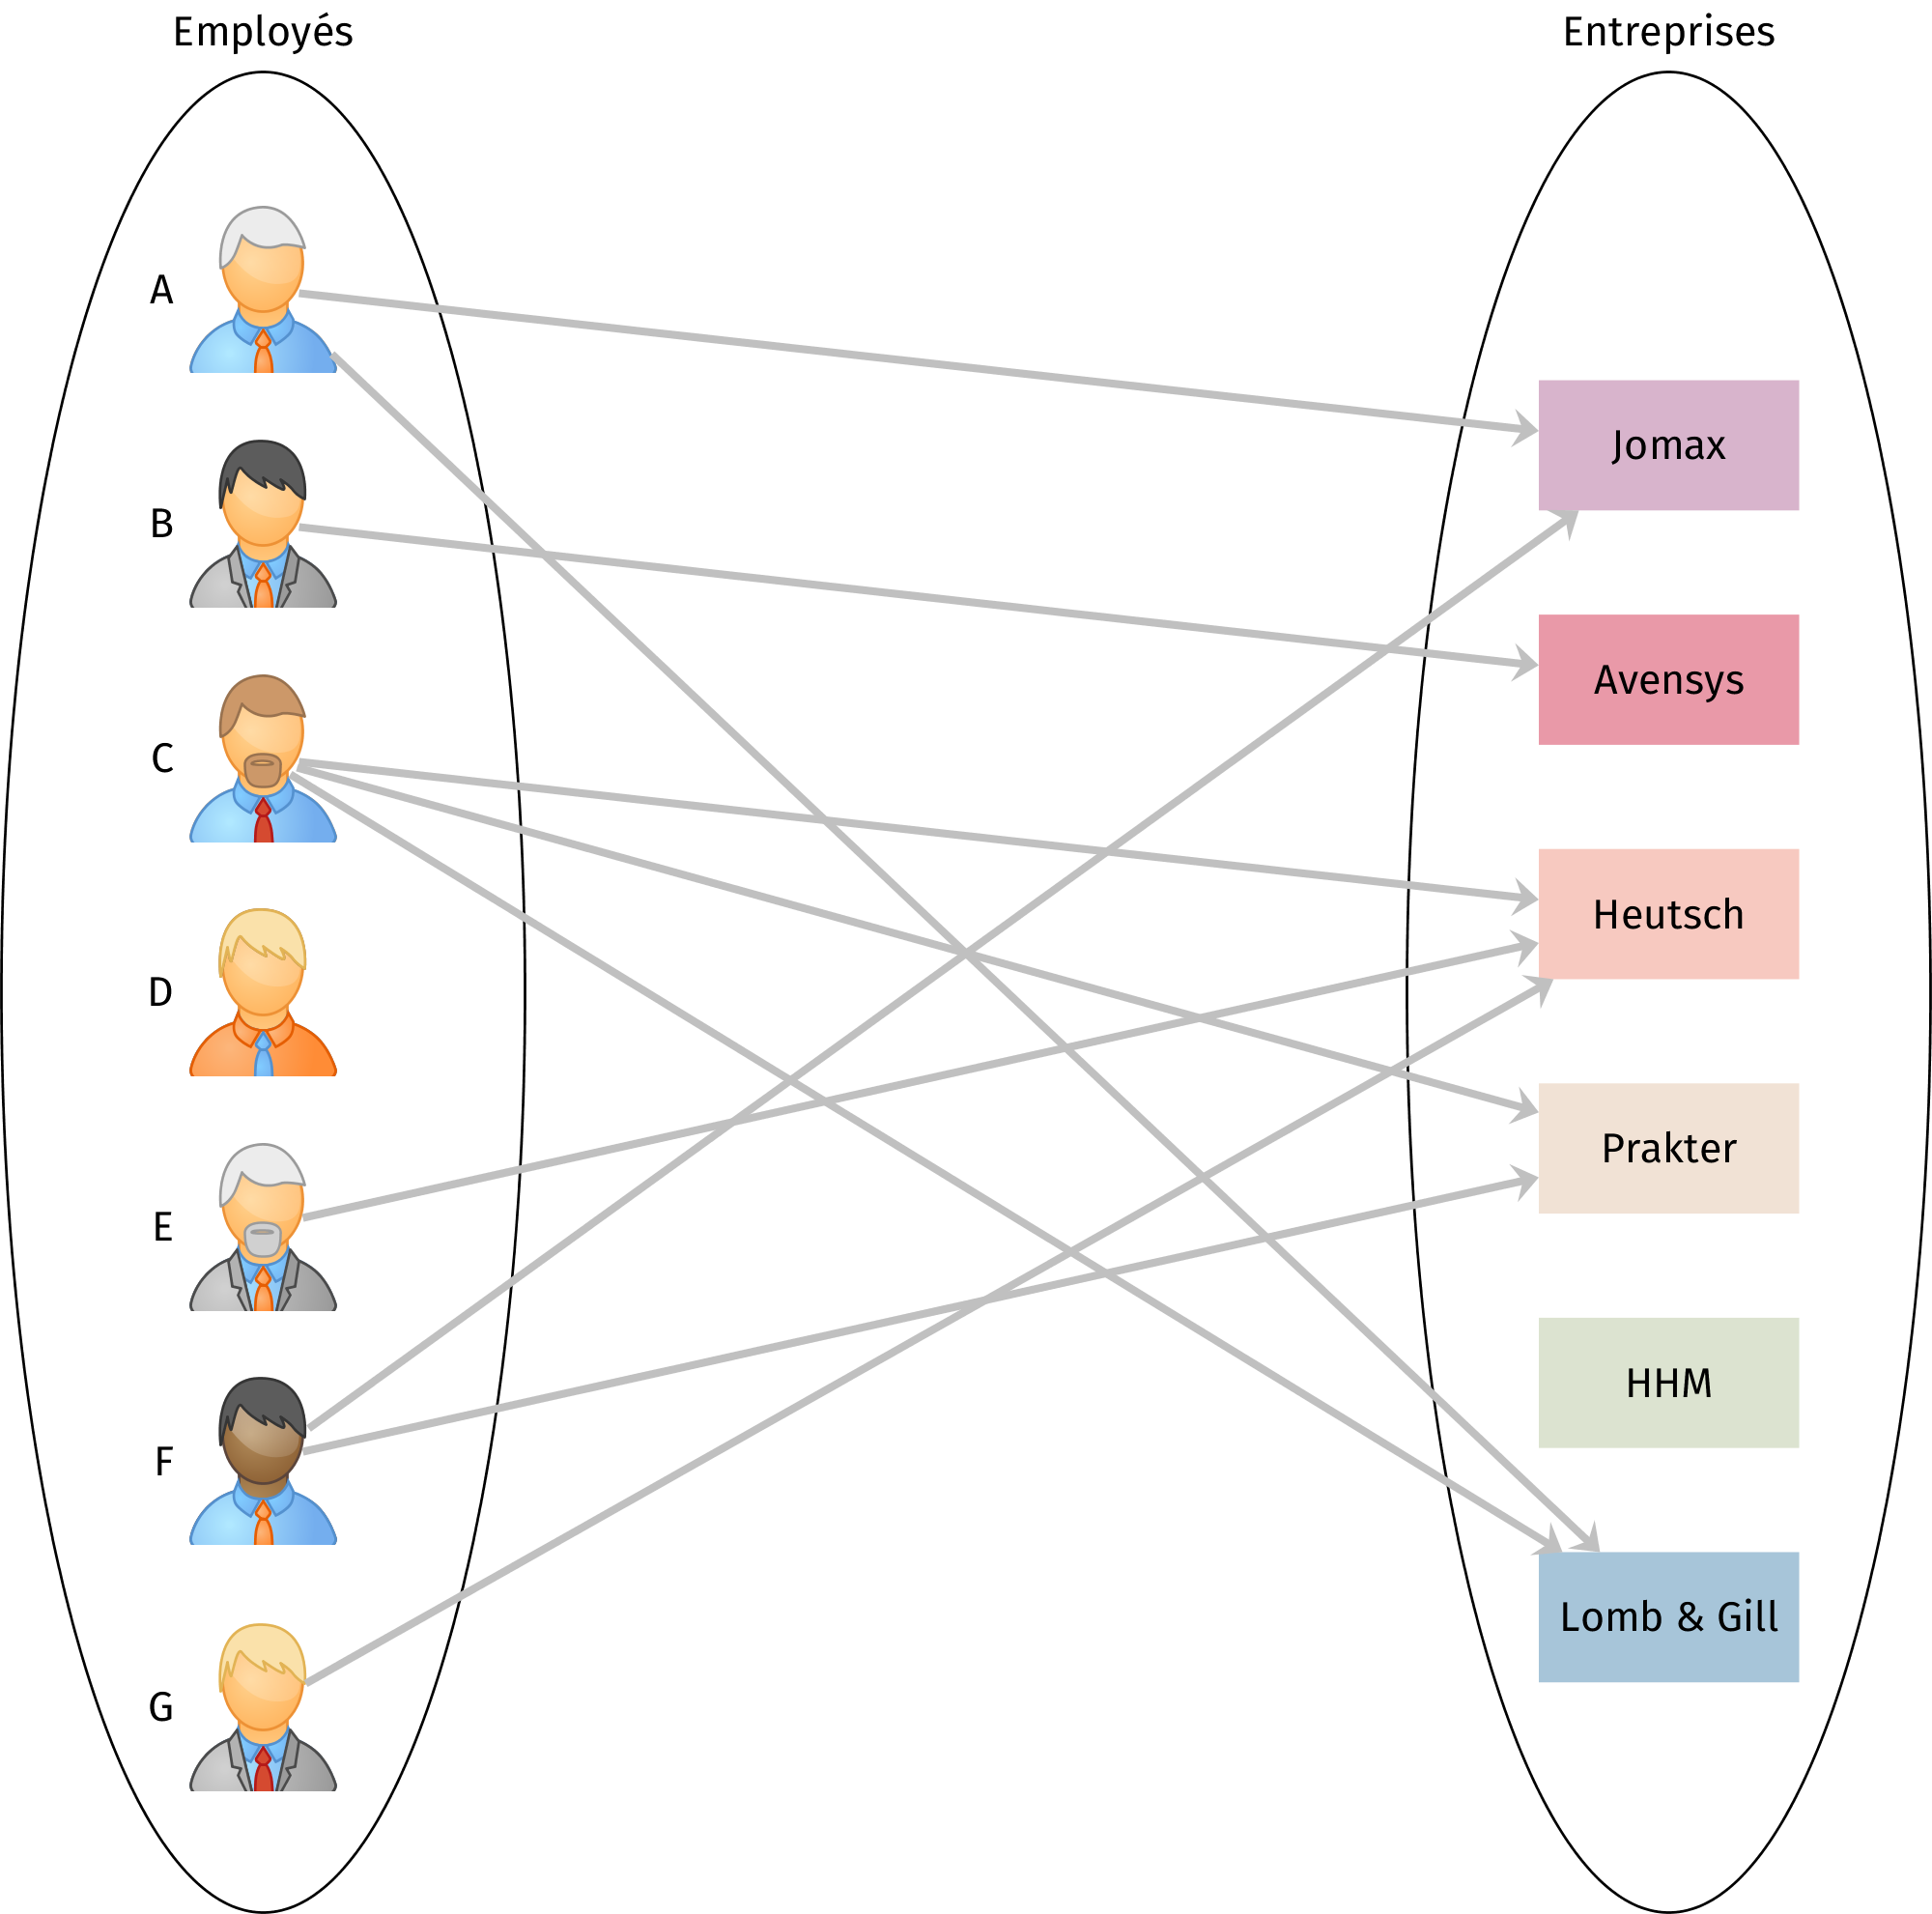
\includegraphics[width=9cm]{ensembles/img/graphe_relation_binaire.png}
    \end{center}
    On considère un ensemble $E$ d'employés, un ensemble $F$ d'entreprises et la relation « ... est ou a été un employé de ... » .
    \begin{itemize}
        \item 	$(A;\,Jomax)\in G$ : l'employé $A$ a travaillé pour l'entreprise Jomax;
        \item 	on a aussi $(A;\,Lomb\,\&\,Gill)\in G$ car cet employé a aussi occupé un poste là-bas;
        \item 	$D$ n'a pas occupé de postes dans $F$.
        \item 	HHM n'a aucun employé de $E$.
    \end{itemize}
    $G$ est ici représenté par l'ensemble des flèches.
\end{exemple}

\begin{exemple}[ : avec un tableau]

    Voici la même relation :\\
    \begin{center}
        \tabstyled
        \begin{tabular}{|l|>{\centering\arraybackslash}m{.7cm}|>{\centering\arraybackslash}m{.7cm}|>{\centering\arraybackslash}m{.7cm}|>{\centering\arraybackslash}m{.7cm}|>{\centering\arraybackslash}m{.7cm}|>{\centering\arraybackslash}m{.7cm}|>{\centering\arraybackslash}m{.7cm}|}
            \hline
            \cellcolor{white}                     & \cellcolor{UGLiBlue}\ccell A & \cellcolor{UGLiBlue}\ccell B & \cellcolor{UGLiBlue}\ccell C & \cellcolor{UGLiBlue}\ccell D & \cellcolor{UGLiBlue}\ccell E & \cellcolor{UGLiBlue}\ccell F & \cellcolor{UGLiBlue}\ccell G \\
            \hline
            \cellcolor{UGLiBlue}\ccell Jomax        & x                          &                            &                            &                            &                            & x                          &                            \\
            \hline
            \cellcolor{UGLiBlue}\ccell Avensys      &                            & x                          &                            &                            &                            &                            &                            \\
            \hline
            \cellcolor{UGLiBlue}\ccell Heutsch      &                            &                            & x                          &                            & x                          &                            & x                          \\
            \hline
            \cellcolor{UGLiBlue}\ccell Prakter      &                            &                            & x                          &                            &                            & x                          &                            \\
            \hline
            \cellcolor{UGLiBlue}\ccell HHM          &                            &                            &                            &                            &                            &                            &                            \\
            \hline
            \cellcolor{UGLiBlue}\ccell Lomb \& Gill & x                          &                            & x                          &                            &                            &                            &                            \\
            \hline
        \end{tabular}
    \end{center}
\end{exemple}

Nous étudierons plus en détail les relations binaires pour lesquelles l'ensemble de départ et d'arrivée sont les mêmes.

\begin{definition}[ : relation binaire dans un ensemble]
    Quand $E=F$ on parle de \textit{relation binaire dans} $E$.
\end{definition}

\begin{exemple}[s]

    \begin{itemize}
        \item 	L'égalité de deux entiers naturels est une relation binaire dans $\N$.
        \item 	Posons $E=\N^*$ et disons que $x\mathcal{R}y$ si et seulement si $x$ divise $y$. On obtient une relation binaire.
        \item 	Dans l'ensemble $\mathcal{D}$ des droites du plan disons que $d\mathcal{R}d'$ si et seulement si $d\perp d'$. On obtient une relation binaire.
    \end{itemize}
\end{exemple}

\begin{definition}[s : réflexivité, symétrie, antisymétrie, transitivité]
    Soit $\mathcal{R}$ une relation binaire sur E, on dit que $\mathcal{R}$ est
    \begin{itemize}
        \item 	\textit{réflexive} si tout élément est en relation avec lui-même : $\forall x\in E,\, x\mathcal{R}x$;
        \item 	\textit{symétrique} si dès que $x\mathcal{R}y$, cela entraîne $y\mathcal{R}x$ (et vice versa, évidemment);
        \item 	\textit{antisymétrique} si deux éléments différents ne peuvent être en relation « dans les deux sens  » .\\
              Cela revient à dire que si on trouve $x\mathcal{R}y$ et $y\mathcal{R}x$, alors nécessairement $x=y$;
        \item 	\textit{transitive} si lorsque $x\mathcal{R}y$ et $y\mathcal{R}z$ alors on a $x\mathcal{R}z$.
    \end{itemize}
\end{definition}
\begin{exemple}[s]

    $\mathcal{R}$ est réflexive. Tout élément est en relation avec lui même :
    \begin{center}
        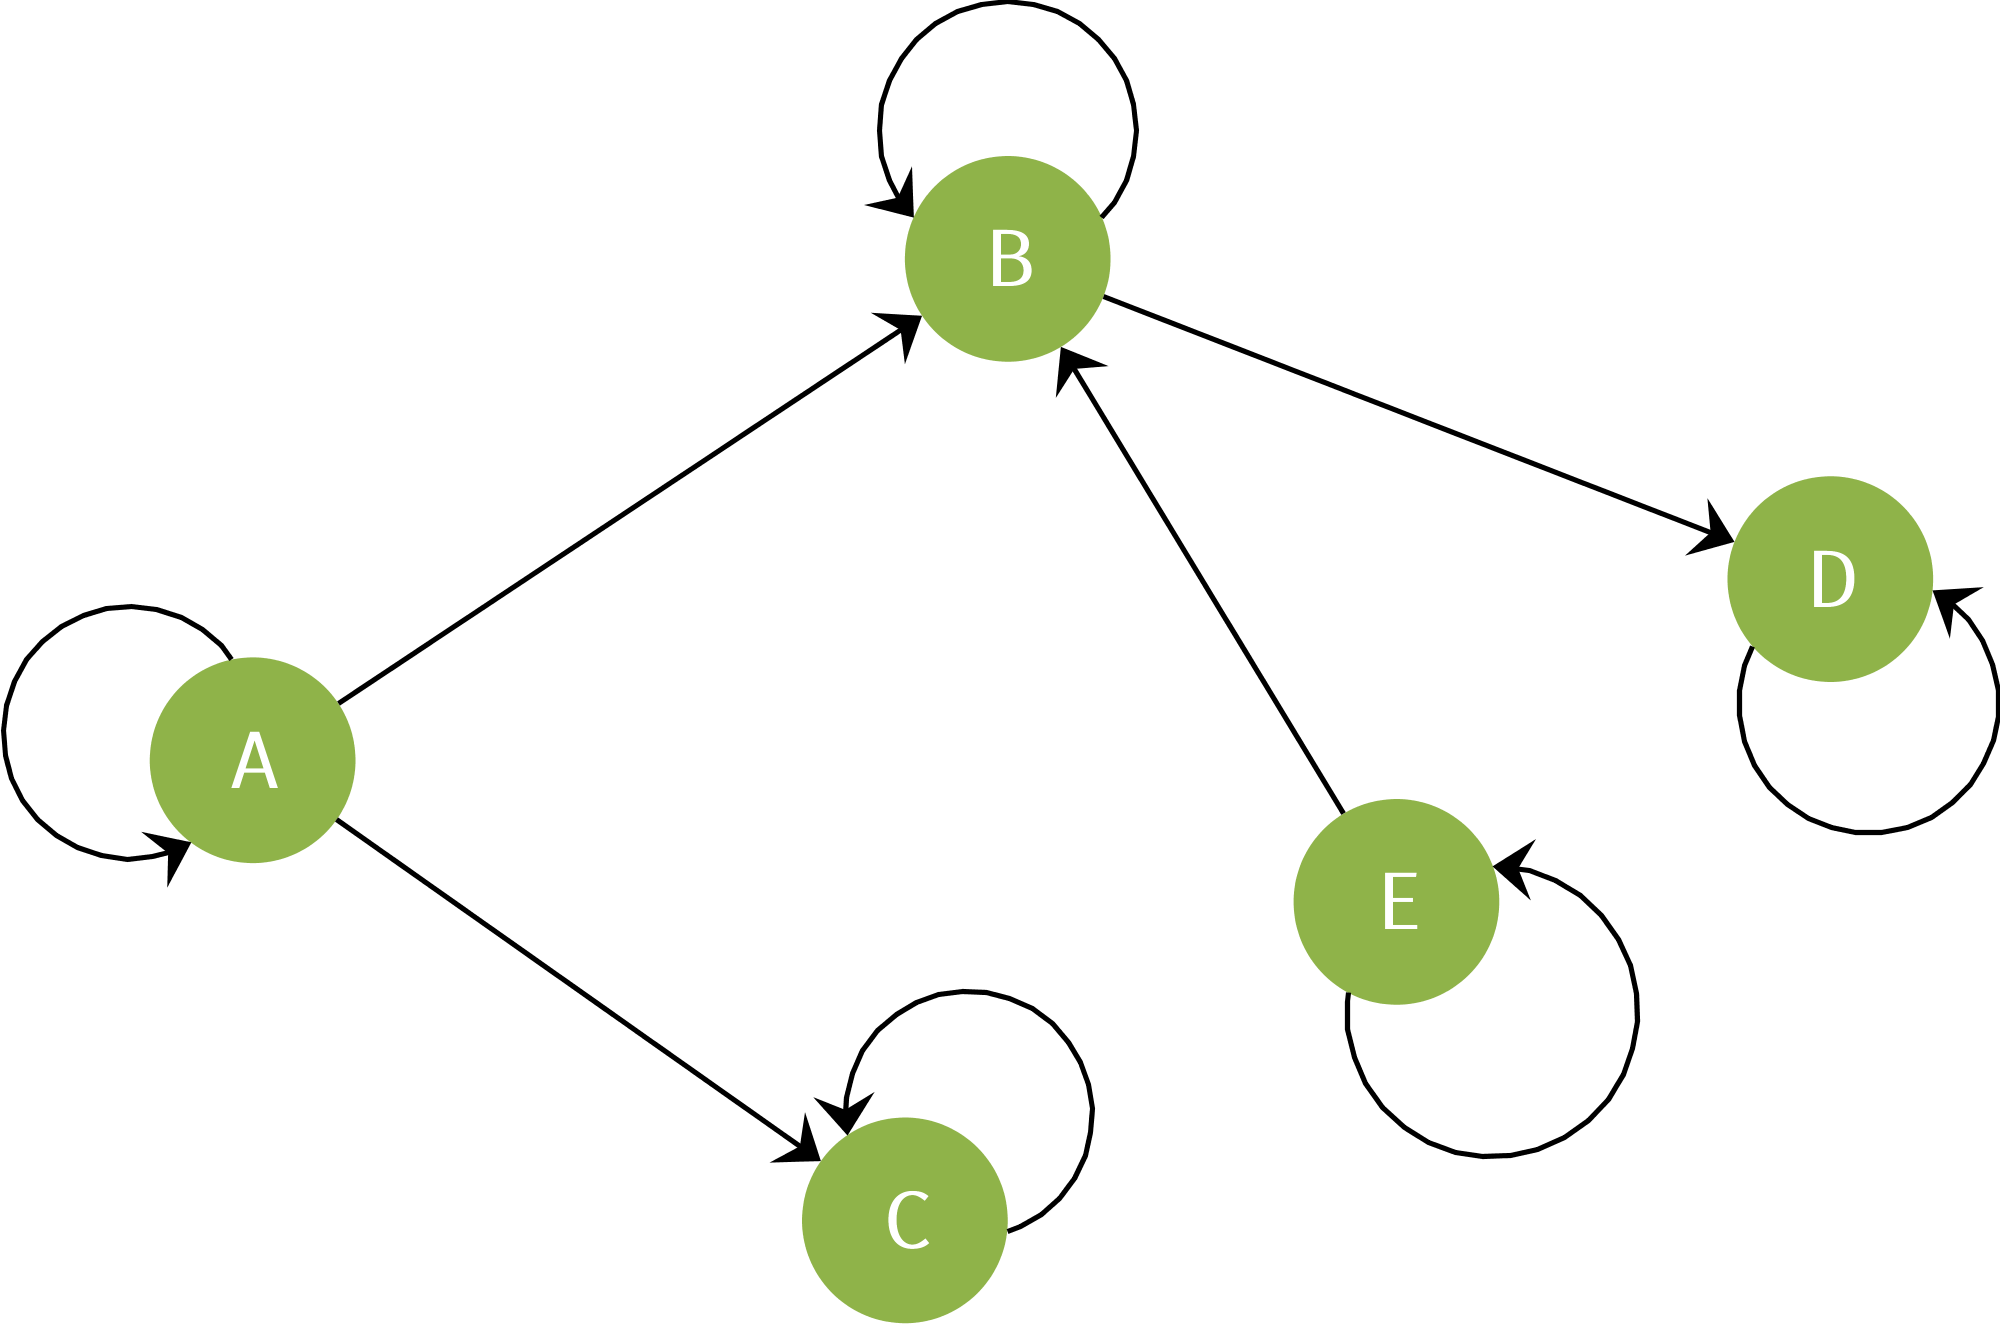
\includegraphics[width=7cm]{ensembles/img/relation_reflexive}
    \end{center}


    $\mathcal{R}$ est symétrique. Si $x\mathcal{R}y$ alors $y\mathcal{R}x$ de sorte que les éléments en relation le sont « dans les deux sens » :

    \begin{center}
        \includegraphics[width=7cm]{ensembles/img/relation_symétrique.png}
    \end{center}


    $\mathcal{R}$ est antisymétrique. Si une relation est vraie « dans les deux sens »  alors c'est qu'elle ne concerne qu'un élément : il n'y a pas de double flèche reliant deux éléments différents mais, peut-être, des cas comme $D\mathcal{R}D$ ou $E\mathcal{R}E$:
    \begin{center}
        \includegraphics[width=7cm]{ensembles/img/relation_antisymétrique.png}
    \end{center}


    $\mathcal{R}$ est transitive. À chaque fois qu'on peut « enchaîner »  les relations, le « raccourci »  est présent aussi :
    \begin{center}
        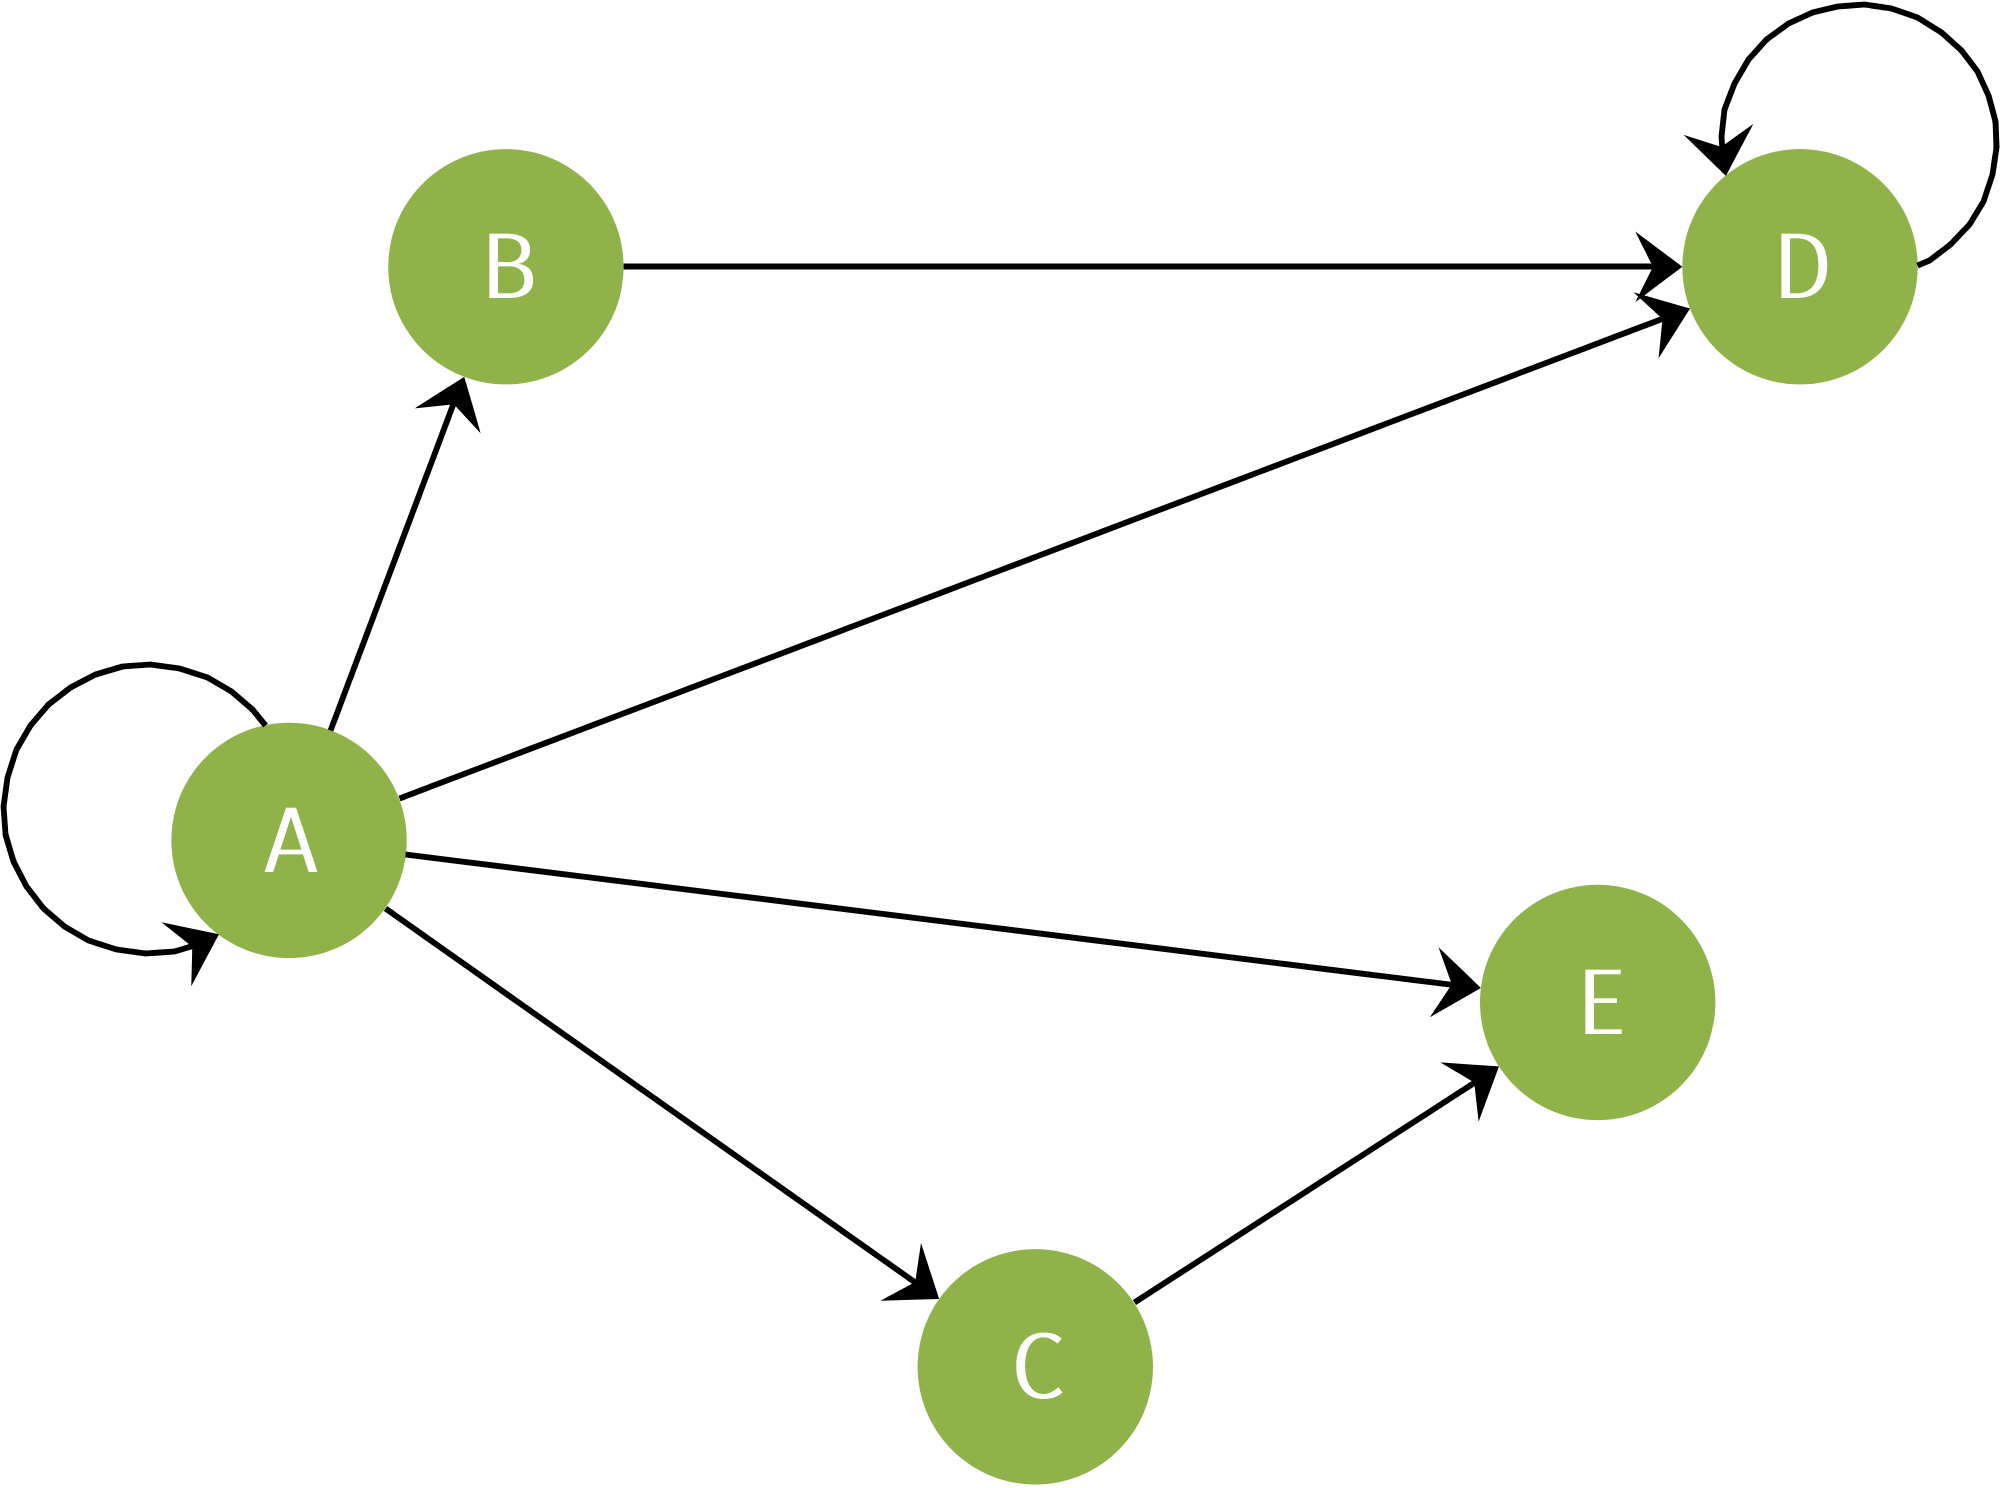
\includegraphics[width=7cm]{ensembles/img/relation_transitive.png}
    \end{center}
\end{exemple}

\begin{definition}[s : relation d'équivalence, relation d'ordre]
    \begin{itemize}
        \item 	Lorsqu'une relation binaire dans E est réflexive, symétrique et transitive, on dit que c'est une relation d'équivalence sur E.\\
              Une relation d'équivalence permet de partager E en \textit{classes} d'éléments qui sont tous équivalents (considérés « pareils »  pour la relation).
        \item 	Lorsqu'une relation binaire dans E est réflexive, antisymétrique et transitive, on dit que c'est une relation d'ordre sur E.\\
              Une relation d'ordre permet de « ranger les éléments comparables  »  :
              \begin{itemize}
                  \item 	Si à chaque fois qu'on prend deux éléments \textit{distincts} $x$ et $y$ alors on a $x\mathcal{R}y$ ou $y\mathcal{R}x$ alors l'ordre est dit \textit{total} car on peut toujours comparer deux éléments différents.
                  \item 	Si ce n'est pas le cas on parle d'ordre partiel.
              \end{itemize}
    \end{itemize}
\end{definition}

\begin{exemple}[s]
    \begin{itemize}
        \item 	Dans $N$, la relation d'égalité est une relation d'équivalence.
        \item 	Dans $\R$ la relation $\leqslant$ est une relation d'ordre totale.
        \item 	Dans l'ensemble des droites du plan, la relation de parallélisme est une relation d'équivalence.
        \item 	On considère $\R^2$ et on l'identifie à l'ensemble des points du plan muni d'un repère $\repaff$.
              On décide de noter $\preceq$ la relation suivante :\\ $(x_1,y_1)\preceq(x_2,y_2)$ si et seulement si $x_1\leqslant x_2$ et $y_1\leqslant y_2$.
              \begin{center}
                  \begin{tikzpicture}[]
                      \draw[fill=white](-1,-1) rectangle (7,7);
                      \repereal{-1}{-1}{7}{7}
                      \pointc{2}{6}{2}{4}{A}
                      \pointc{1}{2}{1}{2}{B}
                      \pointc{5}{3}{5}{3}{C}
                  \end{tikzpicture}
              \end{center}
    \end{itemize}
    alors $\preceq$ est une relation d'ordre, mais c'est ordre n'est pas total  : On a bien $\pc{}{1}{2}\preceq\pc{}{2}{4}$ mais on ne peut pas comparer $\pc{}{2}{4}$ et $\pc{}{5}{3}$.
\end{exemple}

\begin{encadrecolore}{Question}{UGLiOrange}
    Dans $\R$, la relation < est-elle une relation d'ordre ?
\end{encadrecolore}

\begin{exercice}[]
    La relation binaire $\mathcal{R}$ est elle réflexive, symétrique, antisymétrique, transitive ? Est-ce une relation d'équivalence ou d'ordre ? Si c'est une relation d'ordre est elle totale ou partielle ?
    \begin{itemize}
        \item 	Dans $\R$, $x\mathcal{R}y\,\Leftrightarrow\, x<y$.
        \item 	Dans $\N$, $x\mathcal{R}y\,\Leftrightarrow\,x$ divise y.
        \item 	Soit E un ensemble, dans $\mathcal{P}(E)$, $A\mathcal{R}B\,\Leftrightarrow\, A\subset B$.
        \item 	Soit E un ensemble, dans $\mathcal{P}(E)$, $A\mathcal{R}B\,\Leftrightarrow\, A\cap B=\emptyset$.\\
    \end{itemize}
\end{exercice}

\begin{exercice}[]
    \begin{center}
        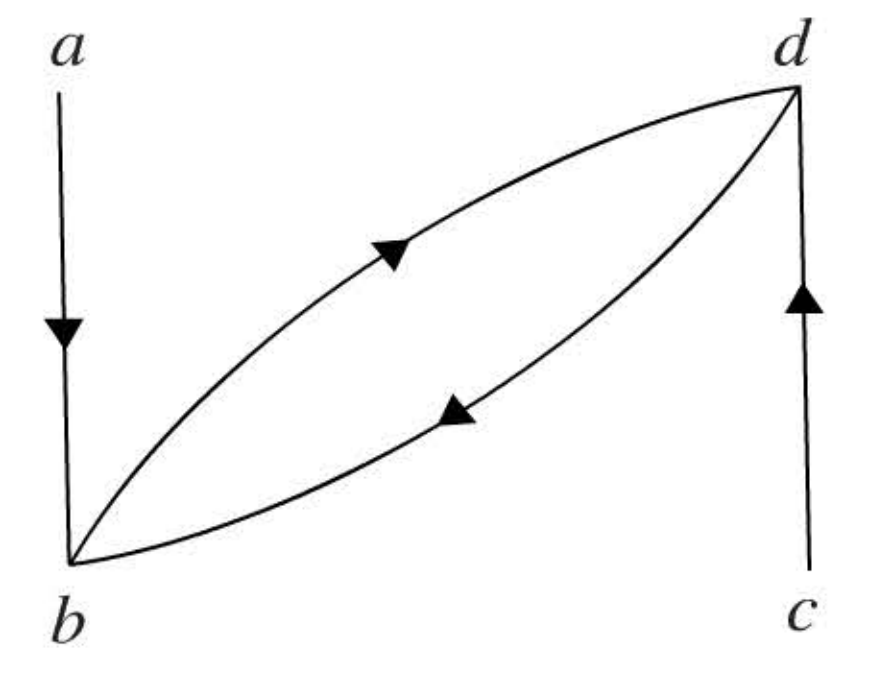
\includegraphics[width=5cm]{ensembles/img/graphe.PNG}
    \end{center}


    On considère le dessin comme étant la représentation d'une relation binaire, que l'on note $\mathcal{R}$ . définie sur l'ensemble $S = \lbrace  a;b;c;d\rbrace$ .

    \begin{enumalph}
        \item 	Écrire tous les éléments qui sont en relation sou s la forme $x\mathcal{R}y$, avec $(x;y) \in S^2$ .
        \item 	La relation R est elle réflexive ?
        \item 	La relation R est elle symétrique ?
        \item 	La relation R est elle transitive ?
        \item 	Au minimum, quelles flèches doit-on ajouter pour obtenir la représentation d'une
        relation réflexive ?
        \item Même question avec une relation symétrique.
    \end{enumalph}
\end{exercice}

\begin{exercice}[]
    On considère l'\textit{arbre binaire suivant} et sur l'ensemble des nombres présents dans l'arbre, on définit une relation binaire : $x\mathcal{R}y$ si et seulement si $x=y$ on bien on peut passer de x à y ou de y à x par un chemin qui descend toujours par la droite.
    \begin{center}
        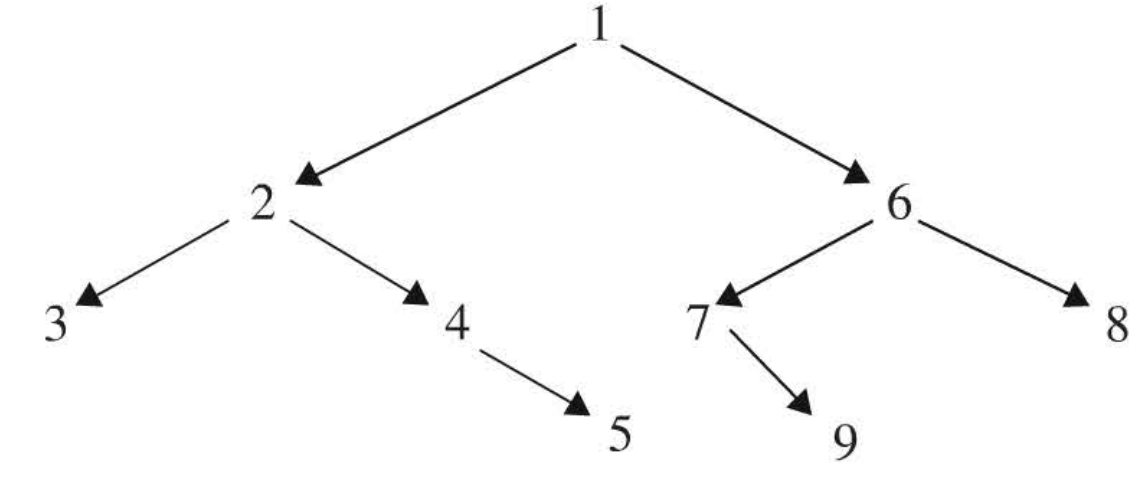
\includegraphics[width=8cm]{ensembles/img/arbre.PNG}
    \end{center}
    \begin{enumerate}
        \item 	Expliquer pourquoi simplement à partir de sa définition on peut affirmer que $\mathcal{R}$ est réflexive et symétrique.
        \item 	Montrer que $\mathcal{R}$ est une relation d'équivalence.
        \item 	Regrouper sur le schéma ci-dessus les nombres équivalents.
    \end{enumerate}
\end{exercice}

\begin{exercice}
    Dire si les relations suivantes sont réflexives, symétriques, antisymétriques, transitives.\\
    Dire ensuite si ce sont des relations d'équivalence, d'ordre total ou partiel.
    \begin{enumerate}
        \item 	Sur $\Z$, $x\mathcal{R}y\ \Longleftrightarrow\  x=-y$.
        \item 	Sur $\R^2$, $(x,\,y)\mathcal{R}(x'\,y')\ \Longleftrightarrow\ x=x'$.
        \item 	Soit $E$ un ensemble, sur $\mathcal{P}(E)$, $X\mathcal{R}Y\ \Longleftrightarrow\ X=Y\ \text{ou}\ X = \barmaj{Y}$.
        \item 	Sur $\Z$, $x\mathcal{R}y\ \Longleftrightarrow\  x+y$ est pair.
        \item 	Soit $E$ un ensemble et $A\subset E$, sur $\mathcal{P}(E)$, $X\mathcal{R}Y\ \Longleftrightarrow\ X\cup A=Y\cup A$.
    \end{enumerate}
\end{exercice}
\section{Applications}

\begin{definition}[s : application image, antécédents]
    Soient $E$ et $F$ deux ensembles. On appelle \textit{application} de $E$ dans $F$ une relation $\mathcal{R}$ binaire de $E$ vers $F$ telle que pour tout élément $x$ de $E$ \textit{il existe un unique} $y$ de $F$ tel que $x\mathcal{R}y$.\\

    L'usage est alors de noter $\mathcal{R}$ comme \textit{une fonction} :
    \begin{tabbing}
        $f\,:\,$ \=	$E\longrightarrow F$\\
        \>	$x \longmapsto y$\ \ où $y$ est l'unique élément de $F$ tel que $x\mathcal{R}y$.
    \end{tabbing}
    Et on écrit que $y=f(x)$.\\

    $y$ est appelé l'\textit{image} de $x$ par l'application $f$.\\
    On dit que $x$ est \textit{un antécédent} de $y$ par $f$.
\end{definition}

\begin{exemple}[s]
    Cette relation binaire n'est pas une application de l'ensemble Employés dans l'ensemble Entreprises car (par exemple), l'élément A est associé à 2 éléments de Entreprises
    \begin{center}
        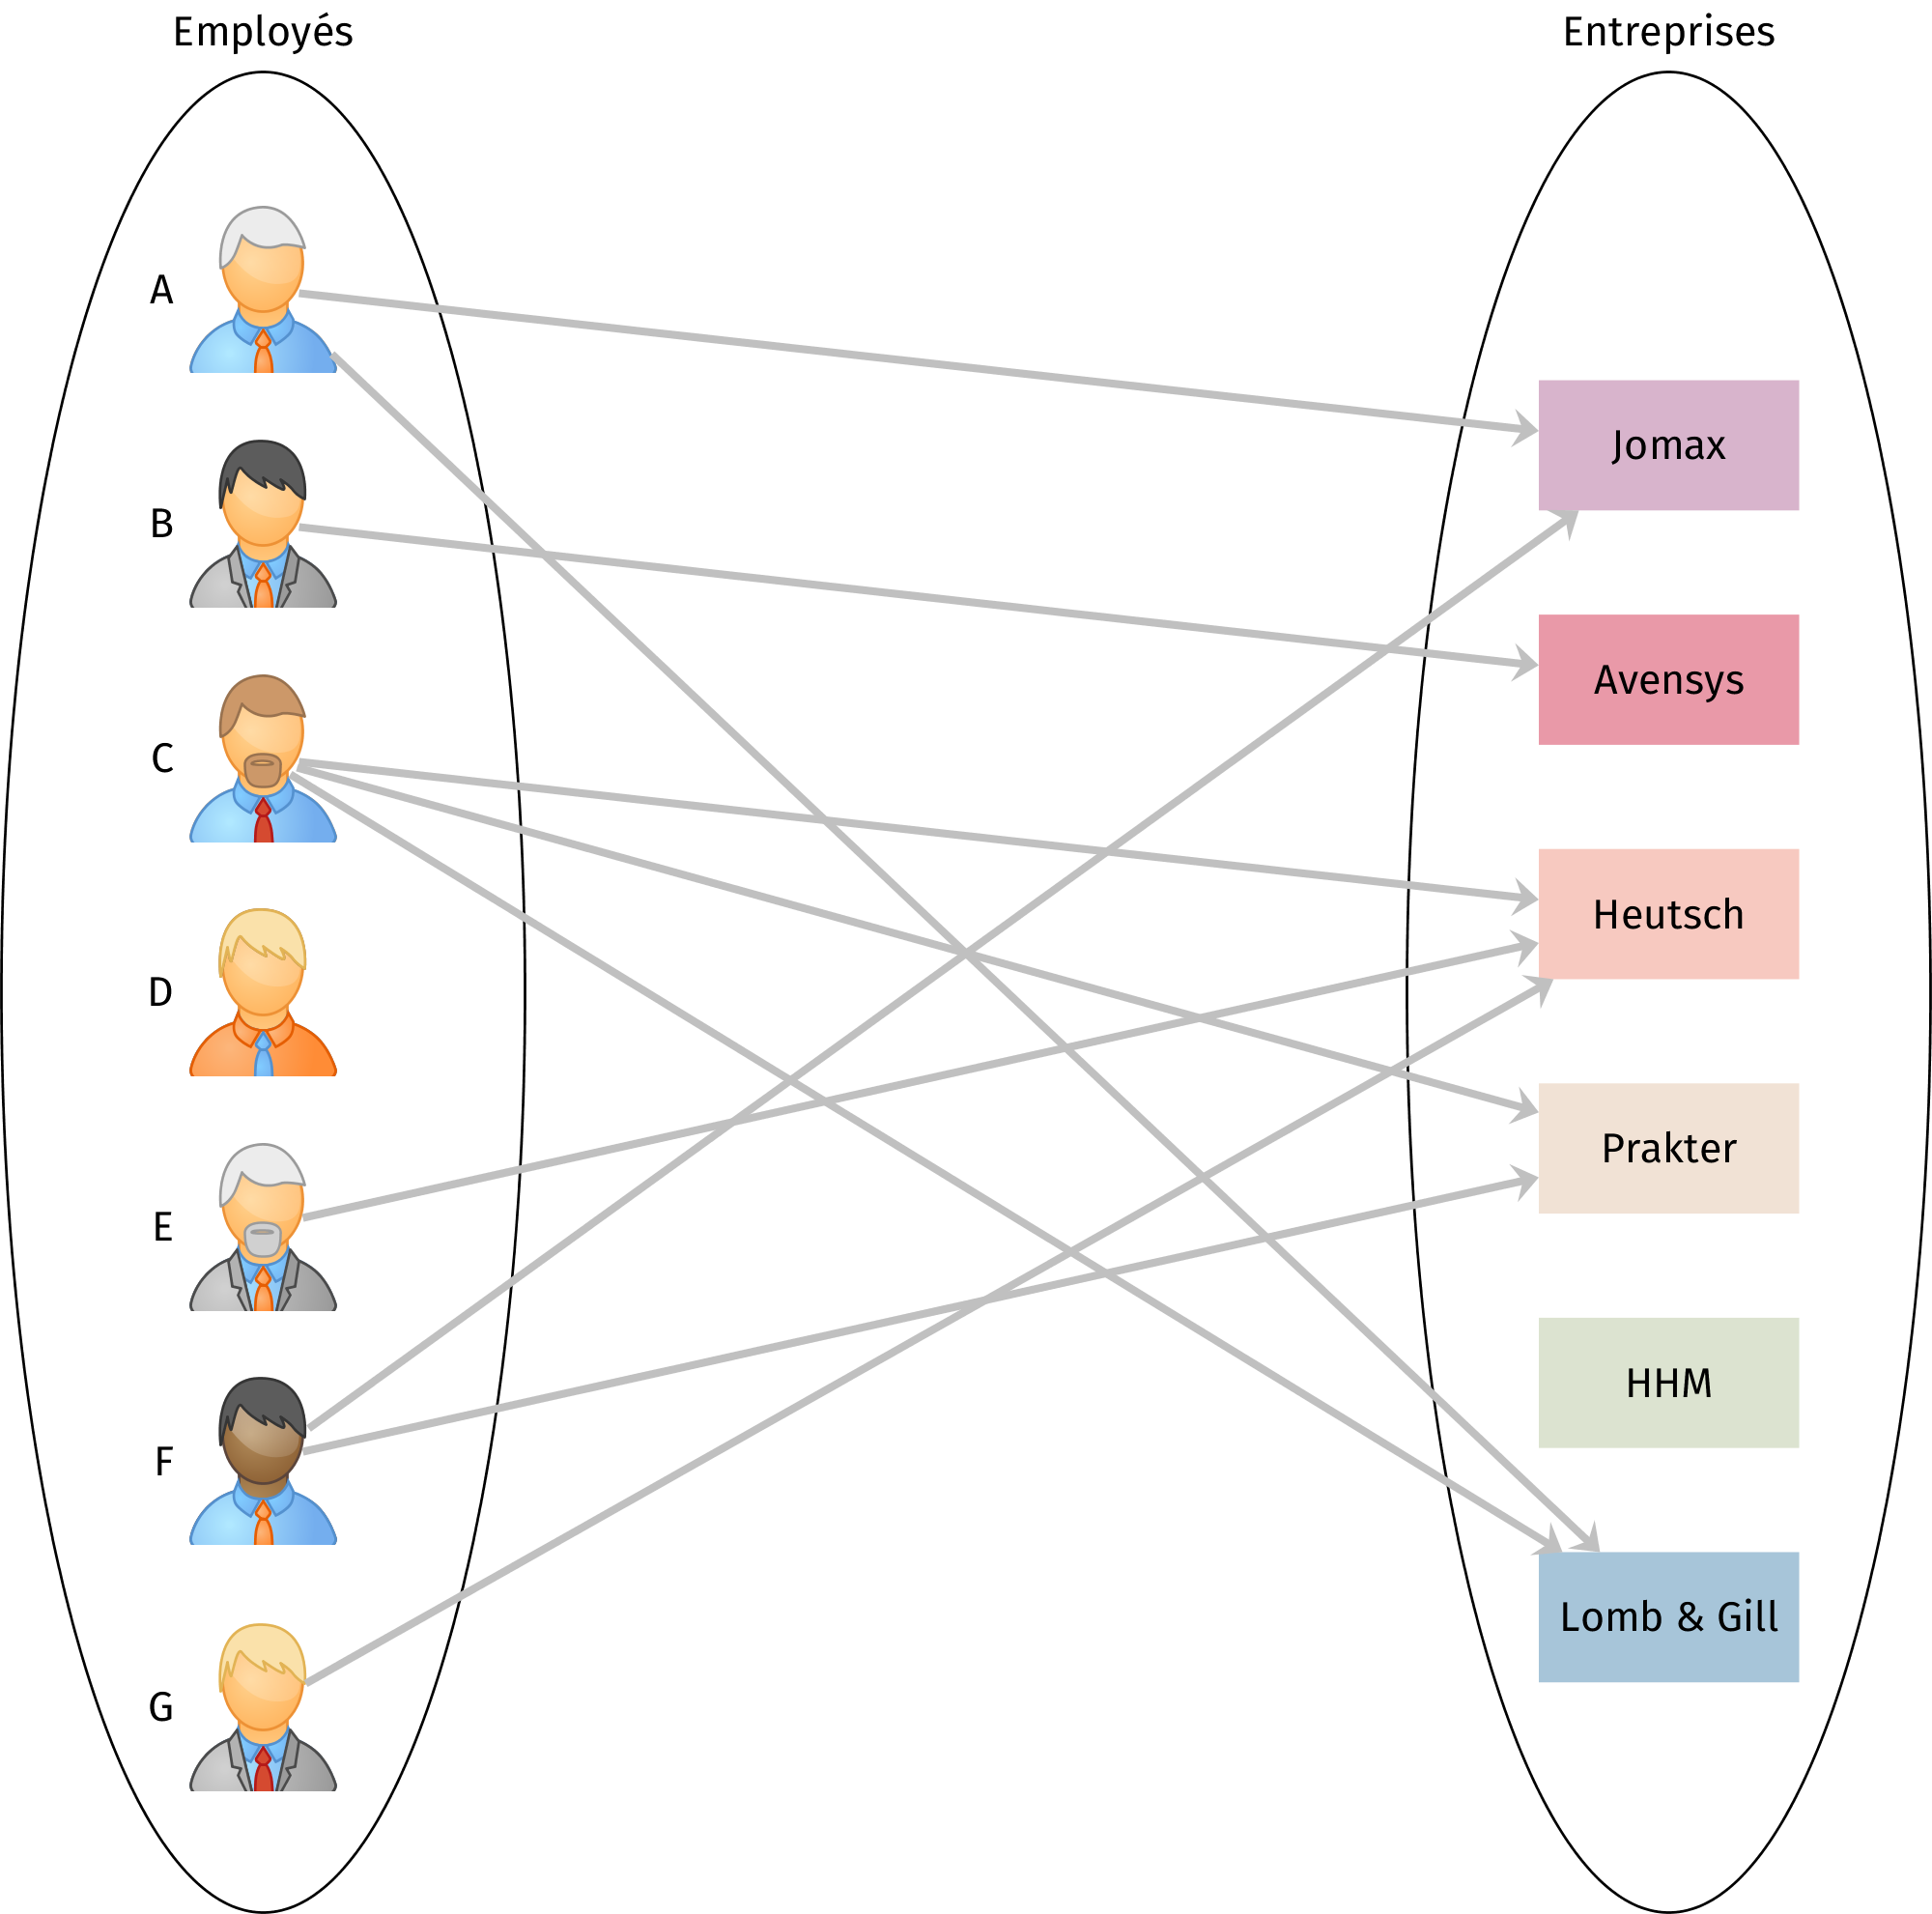
\includegraphics[width=7cm]{ensembles/img/graphe_relation_binaire.png}
    \end{center}
    Celle-ci n'en est pas une non plus car D n'est associé à aucun élément de Entreprises.
    \begin{center}
        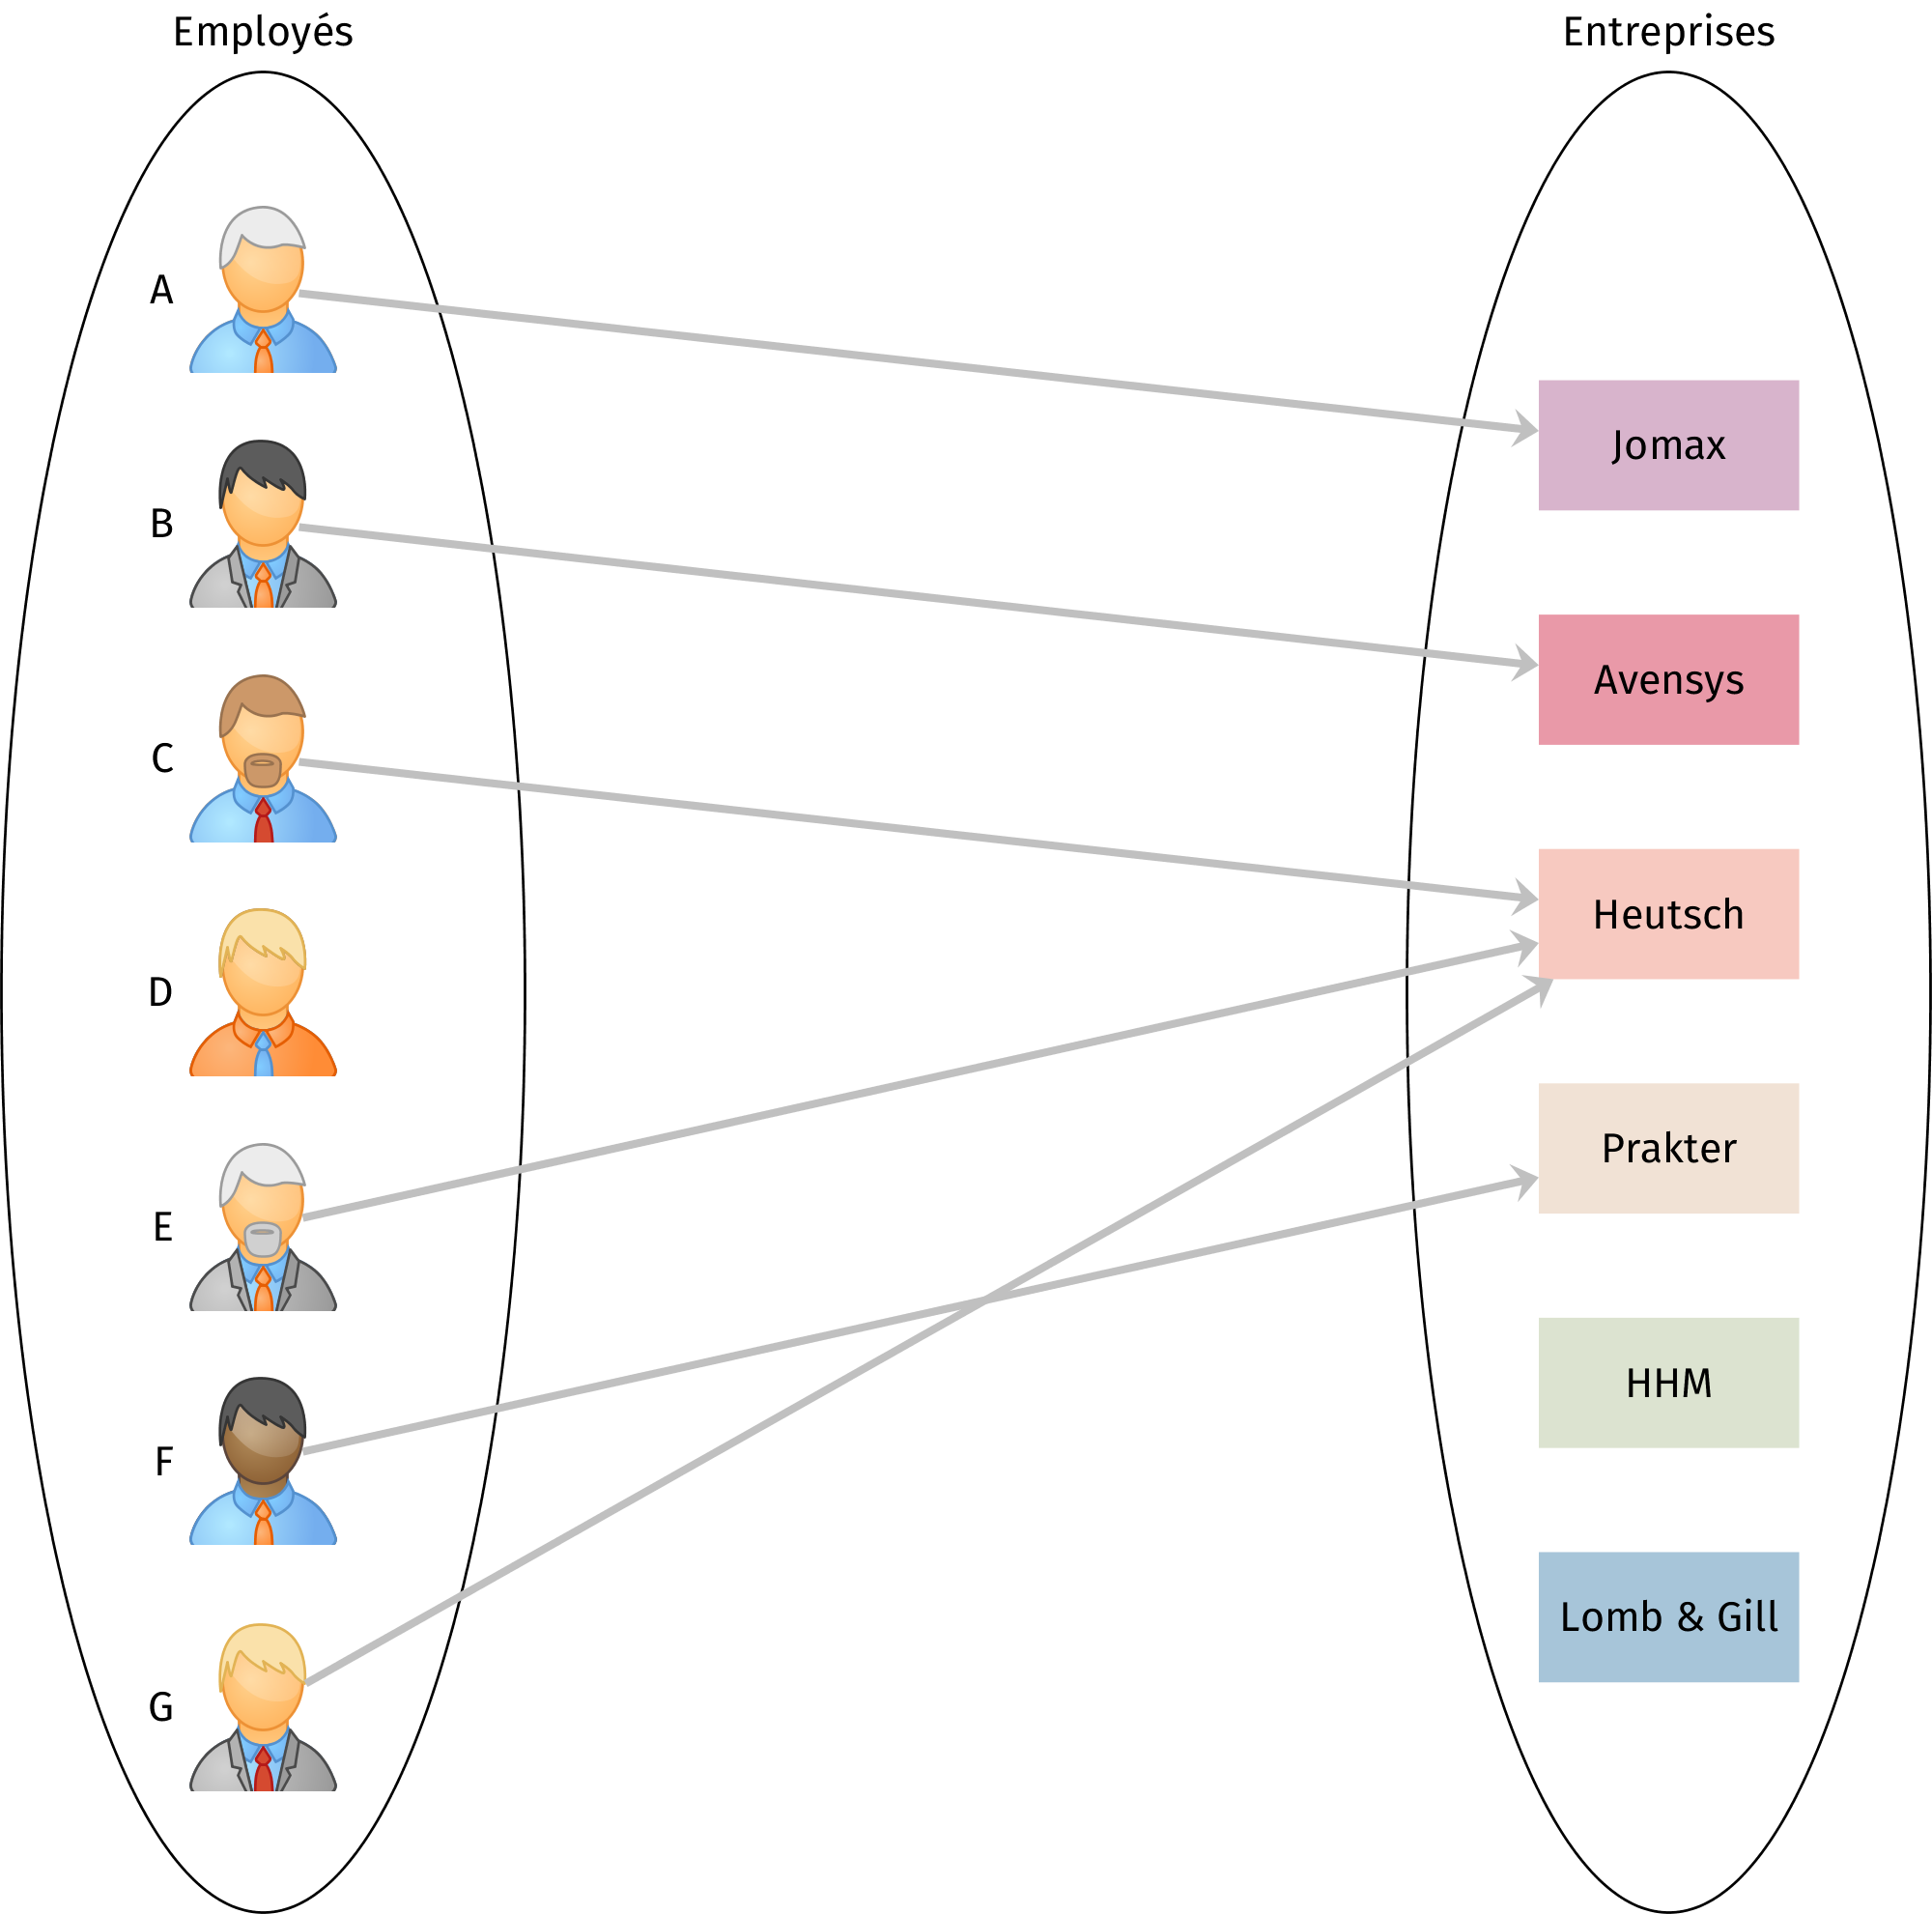
\includegraphics[width=7cm]{ensembles/img/pas_appli.png}
    \end{center}
    Celle-ci en est une car tout élément de Employés est associé à un \textit{unique} élément de Entreprises.
    \begin{center}
        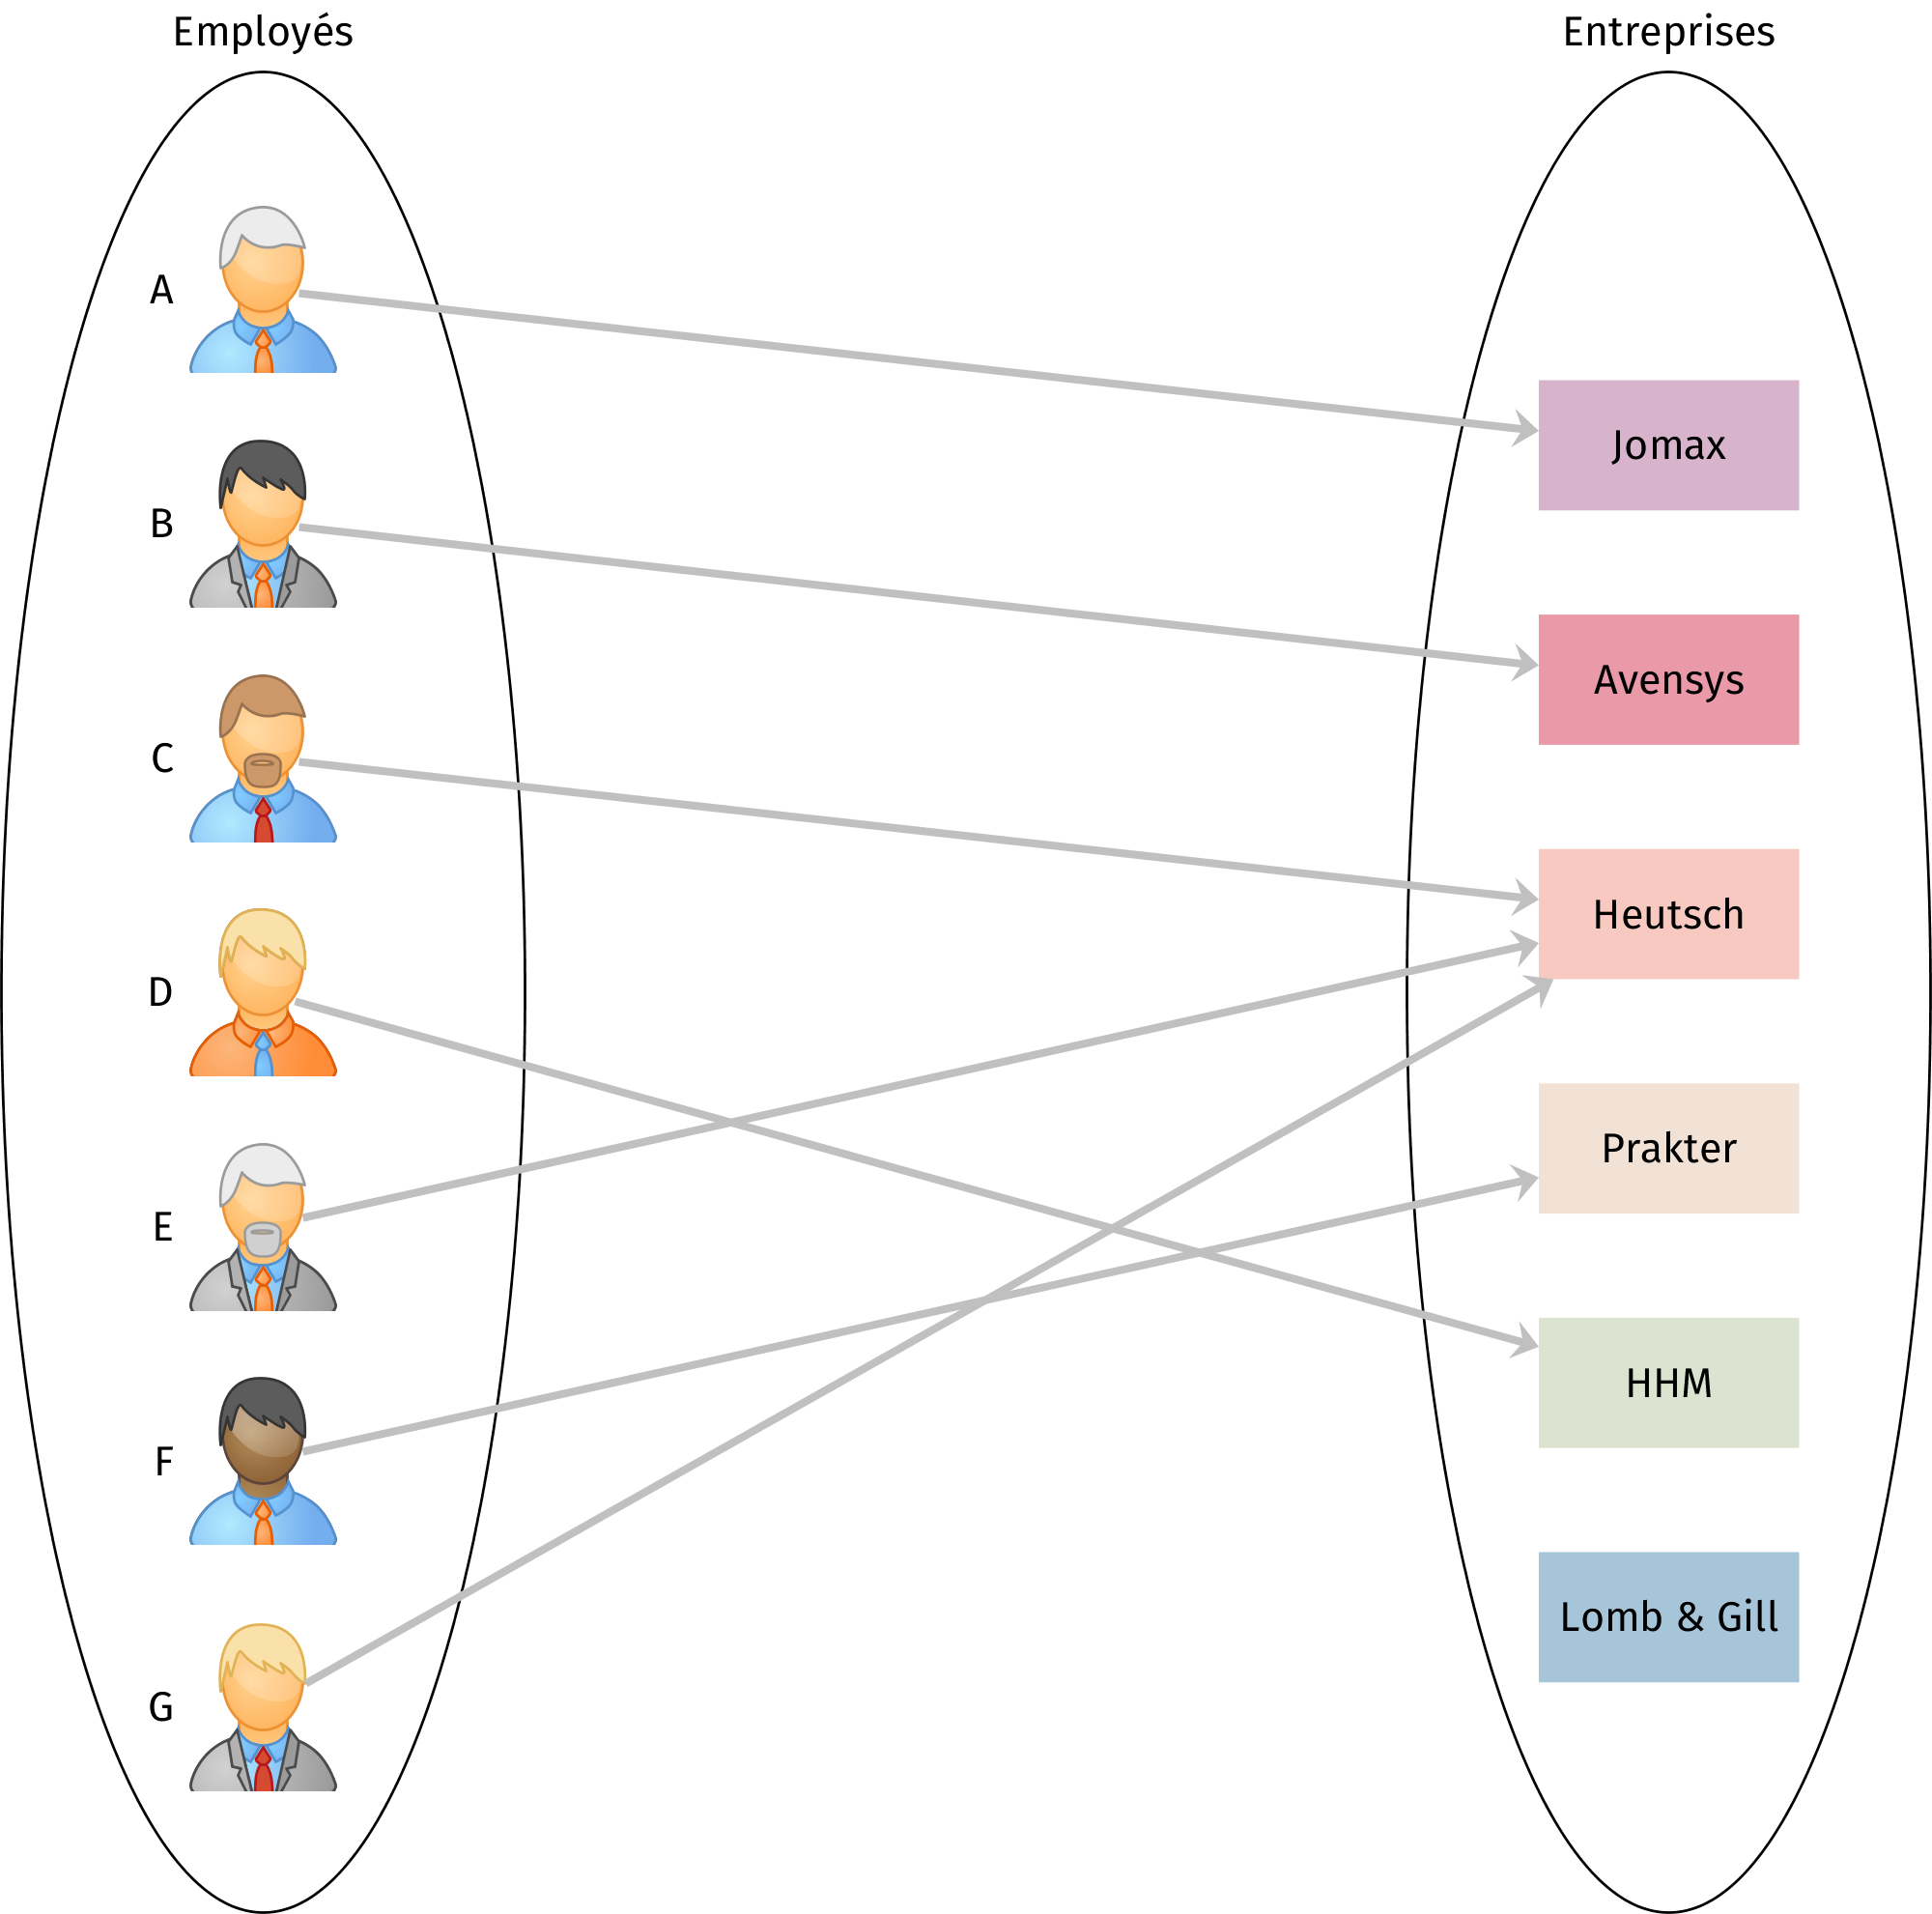
\includegraphics[width=7cm]{ensembles/img/appli.png}
    \end{center}
    Si on décide de l'appeler $f$ alors on écrira :\\$f(A)=Jomax$ et de même $f(B)=Avensys$.
\end{exemple}

\begin{remarque}[]
    Lorsque $f$ est une application de $E$ dans $F$, \textit{tous} les éléments de $E$ ont \textit{une unique image} dans $F$. En revanche, tous les éléments de l'ensemble d'arrivée $F$ n'ont pas obligatoirement un unique antécédent par $f$ : chacun peut en avoir aucun, un seul ou plusieurs.\\
    Dans l'exemple précédent Jomax admet A pour unique antécédent. Heutsch admet 3 antécédents, et Lomb \& Gill n'en a aucun.
\end{remarque}

\begin{definition}[s : injection, surjection, bijection]
    Soit $f$ une application de $E$ dans $F$.
    \begin{itemize}
        \item 	Si tout élément de $F$ admet \textit{au plus} un antécédent par $f$ alors on dit que $f$ est \textit{injective} ou bien que c'est une \textit{injection}.
              \begin{center}
                  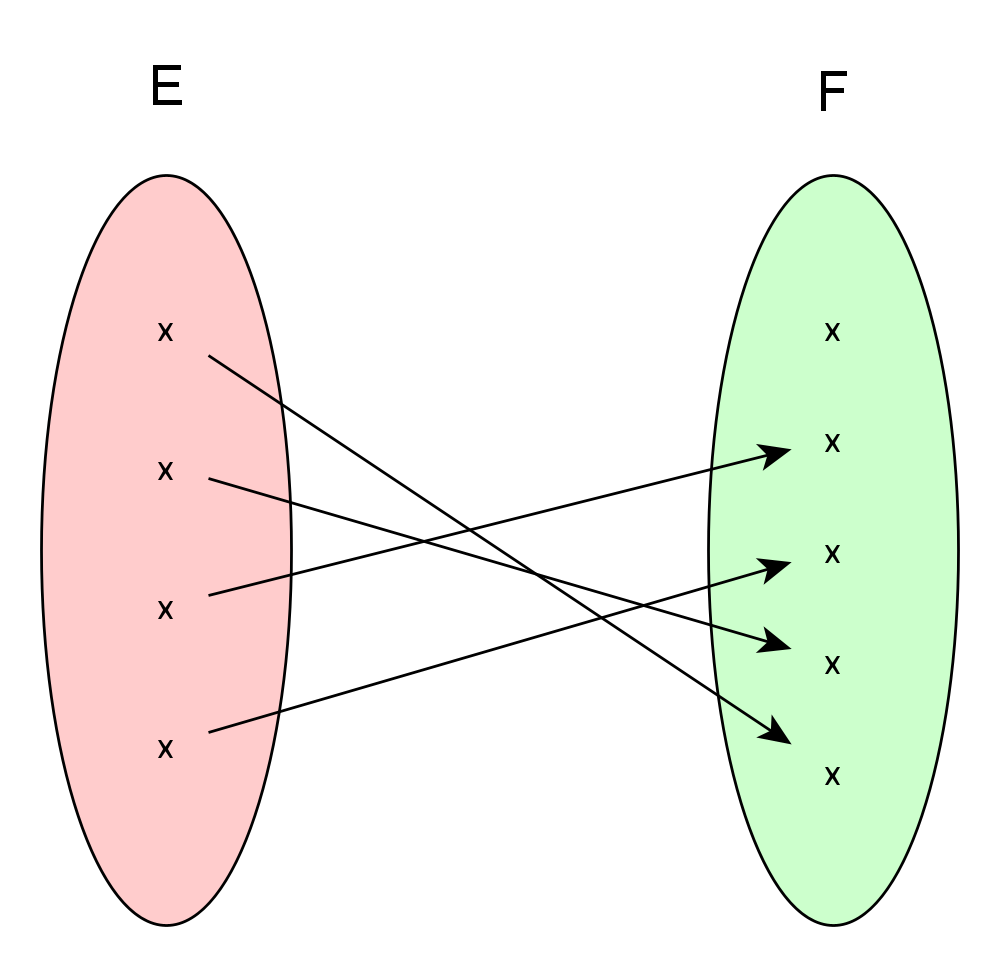
\includegraphics[width=6cm]{ensembles/img/ex_inj.png}\\ {\footnotesize injection de $E$ dans $F$}
              \end{center}
        \item 	Si tout élément de $F$ admet \textit{au moins} un antécédent par $f$ alors on dit que $f$ est \textit{surjective} ou bien que c'est une \textit{surjection}.
              \begin{center}
                  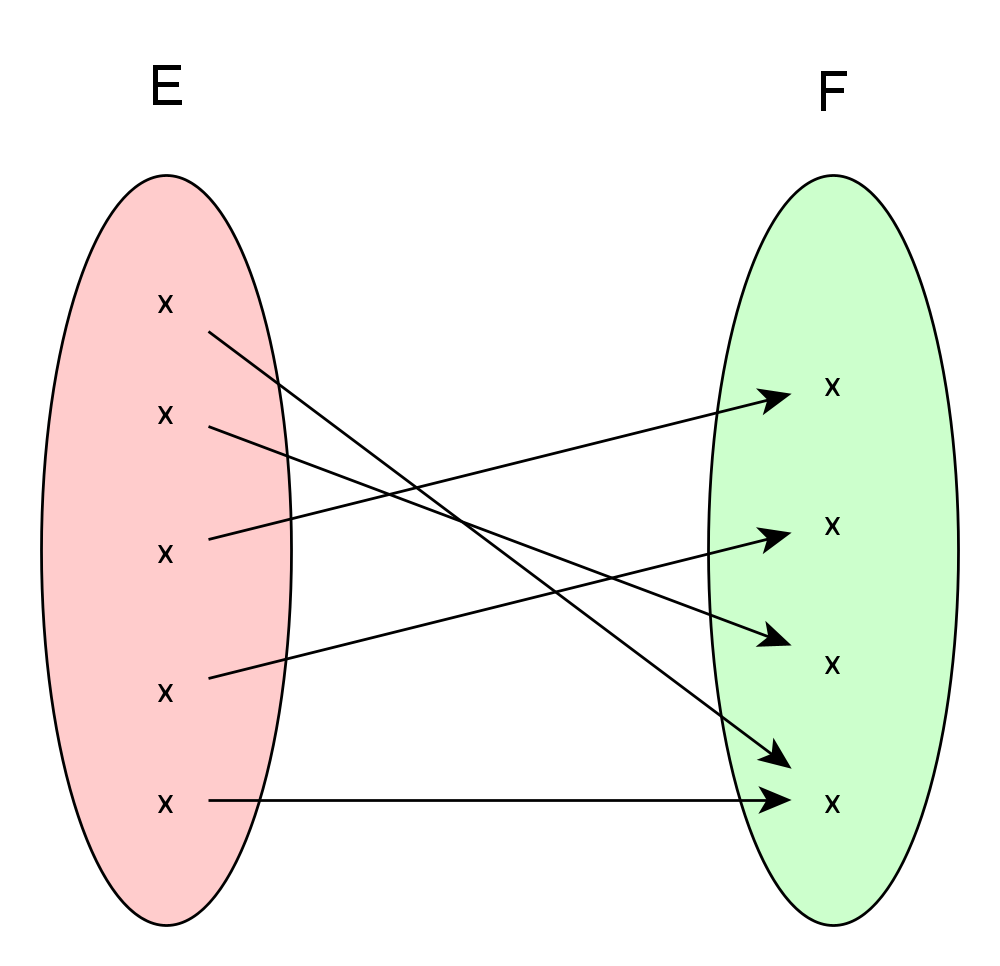
\includegraphics[width=6cm]{ensembles/img/ex_surj.png}\\ {\footnotesize surjection de $E$ dans $F$}
              \end{center}
        \item tout élément de $F$ admet \textit{exactement} un antécédent par $f$ alors  $f$ est \textit{à la fois injective et surjective} et on dit que $f$ est \textit{bijective} ou bien que c'est une \textit{bijection}.
              \begin{center}
                  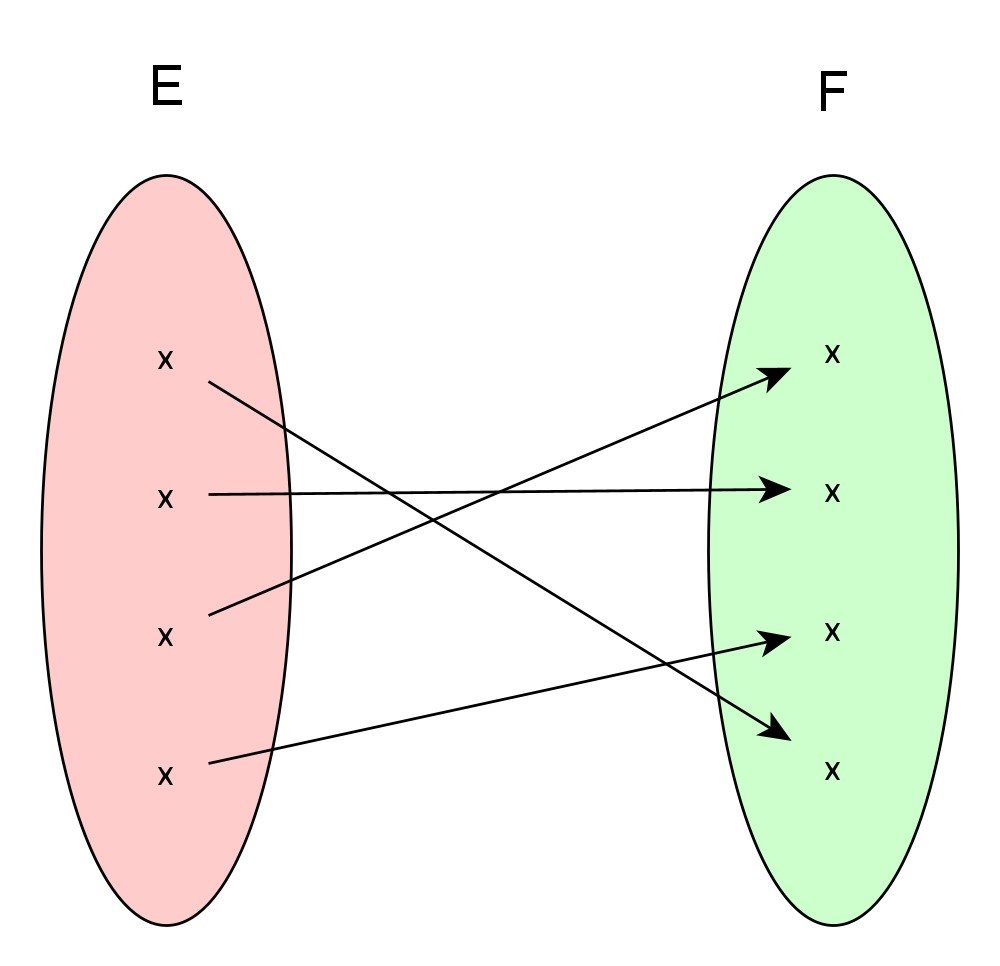
\includegraphics[width=6cm]{ensembles/img/ex_bij.png}\\ {\footnotesize bijection de $E$ dans $F$}
              \end{center}
    \end{itemize}
\end{definition}


\begin{exercice}[]
    Pour chaque relation de E (en rose à gauche) vers F (en vert à droite) indiquer si c'est une application, et si elle est injective, surjective, bijective ou rien du tout.
    \def\myw{5cm}
    \begin{multicols}{2}
        \begin{enumerate}
            \item 	\ \\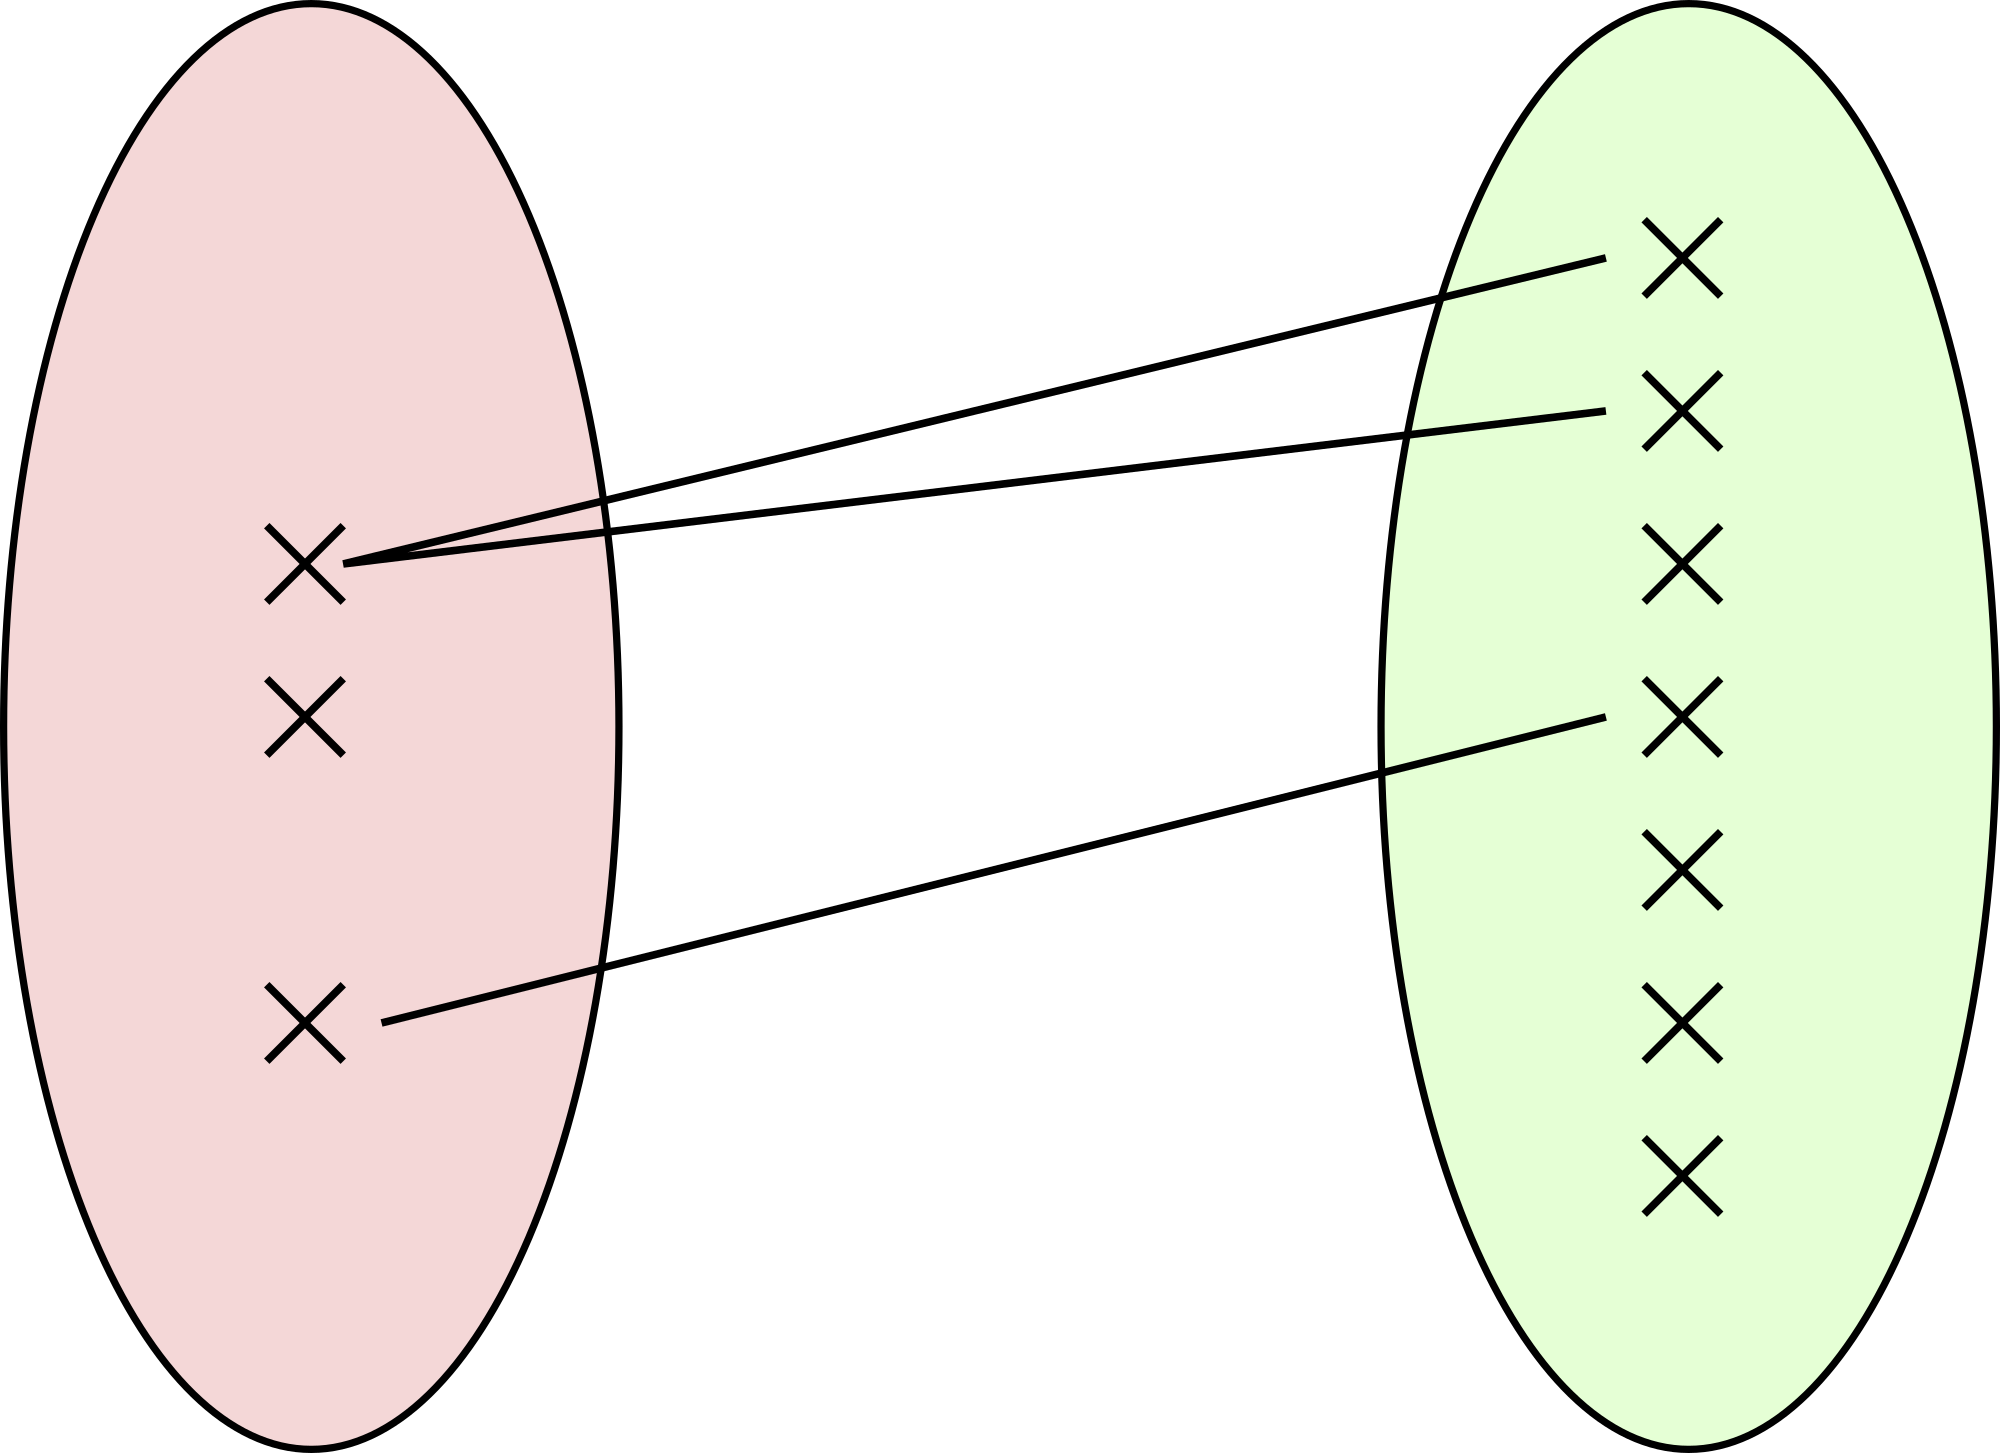
\includegraphics[width=\myw]{ensembles/img/1.png}
            \item 	\ \\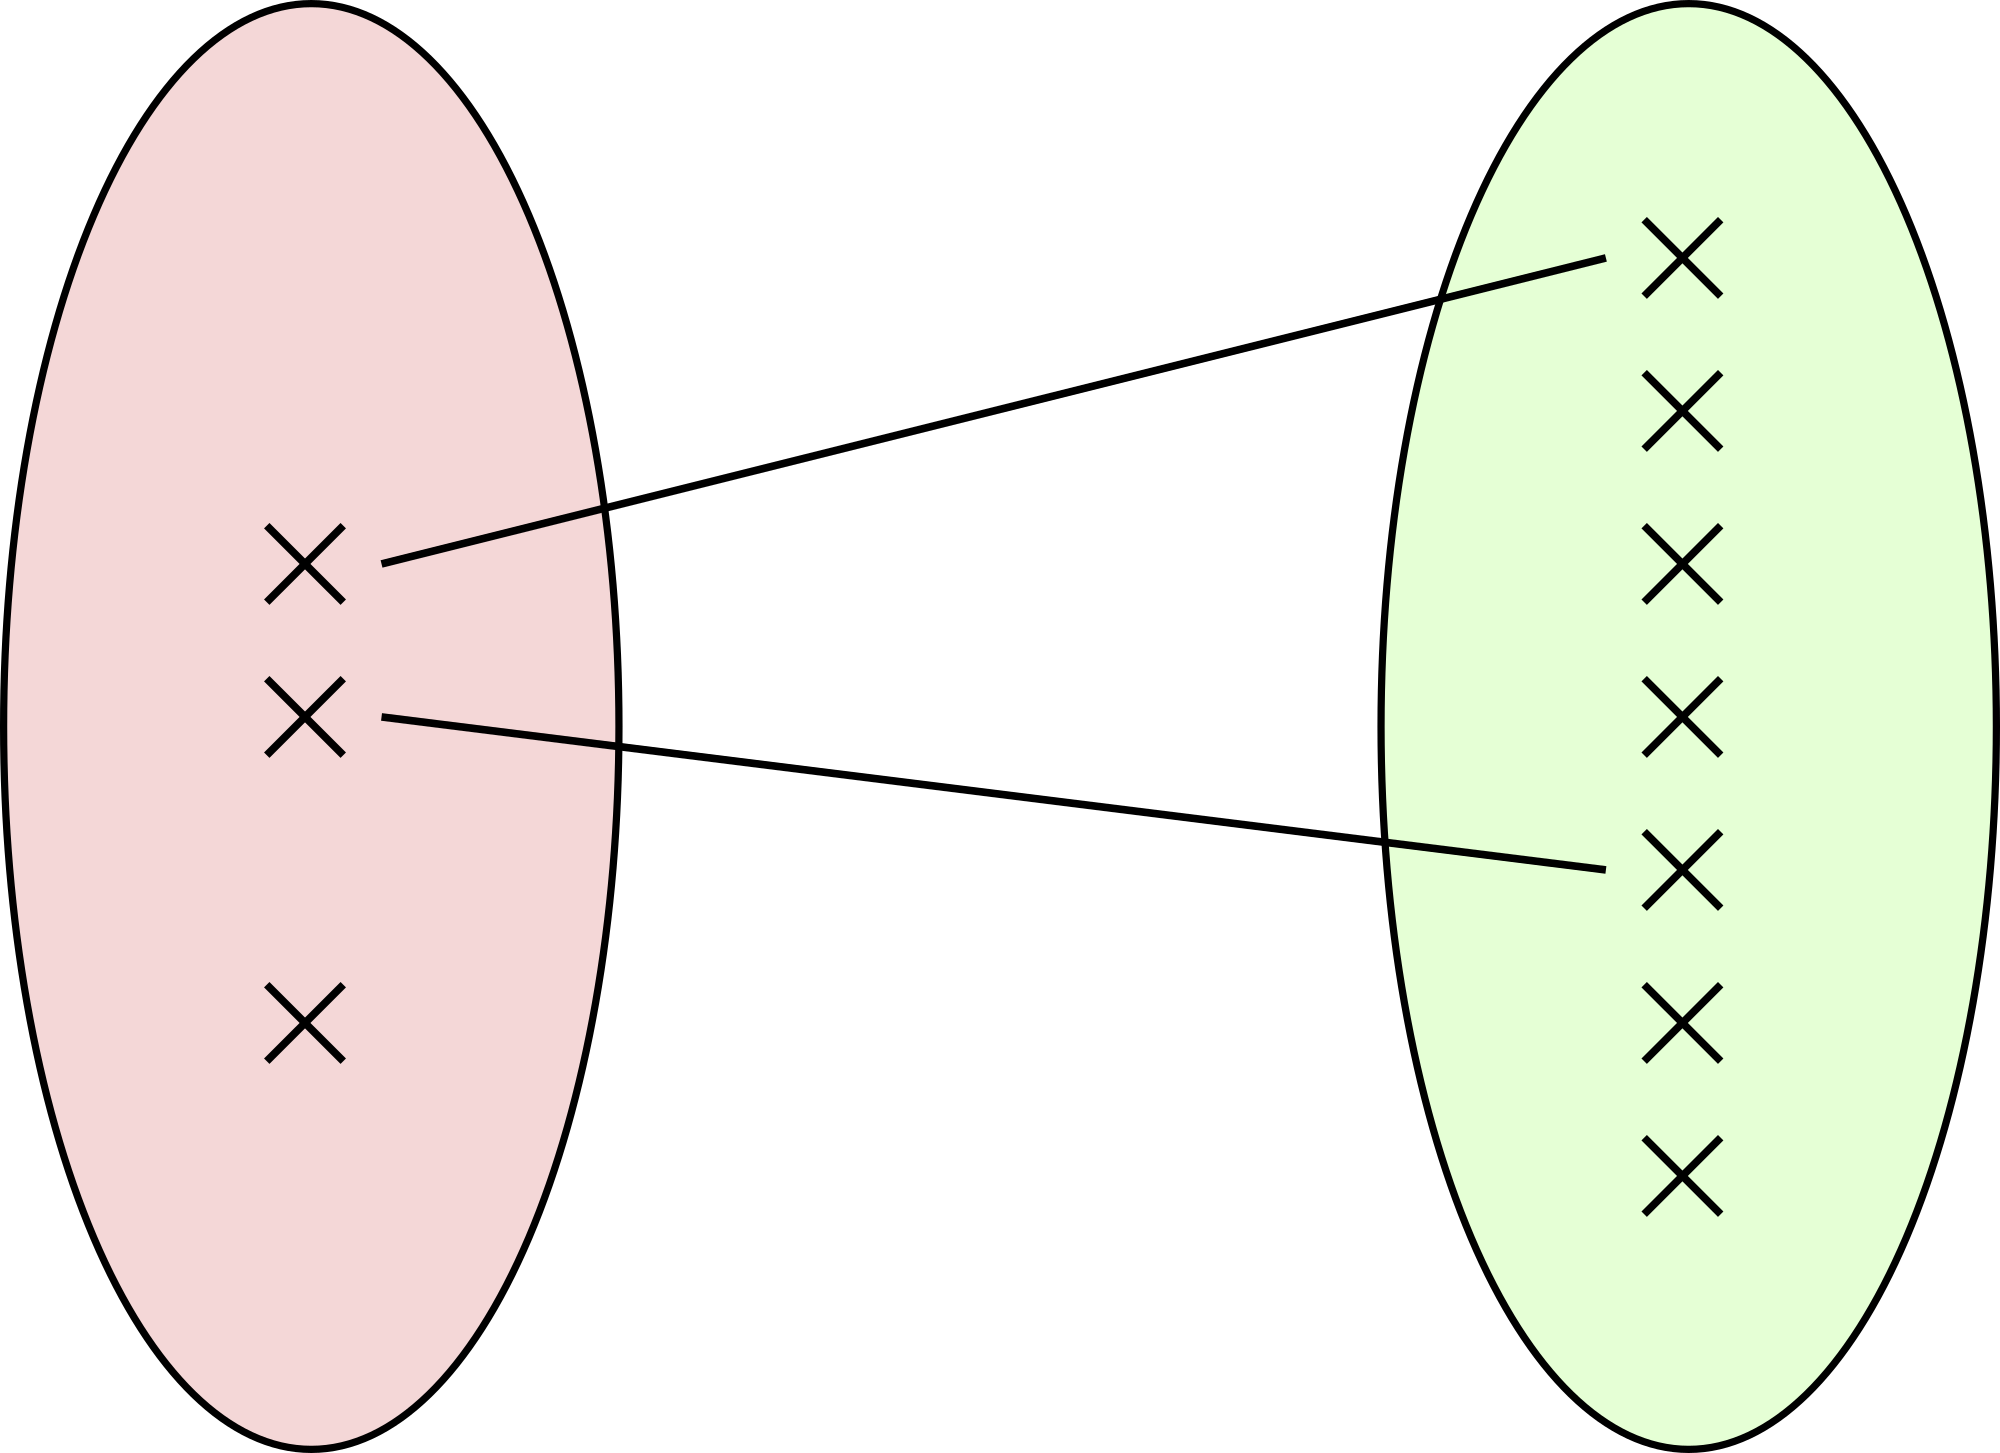
\includegraphics[width=\myw]{ensembles/img/2.png}
            \item 	\ \\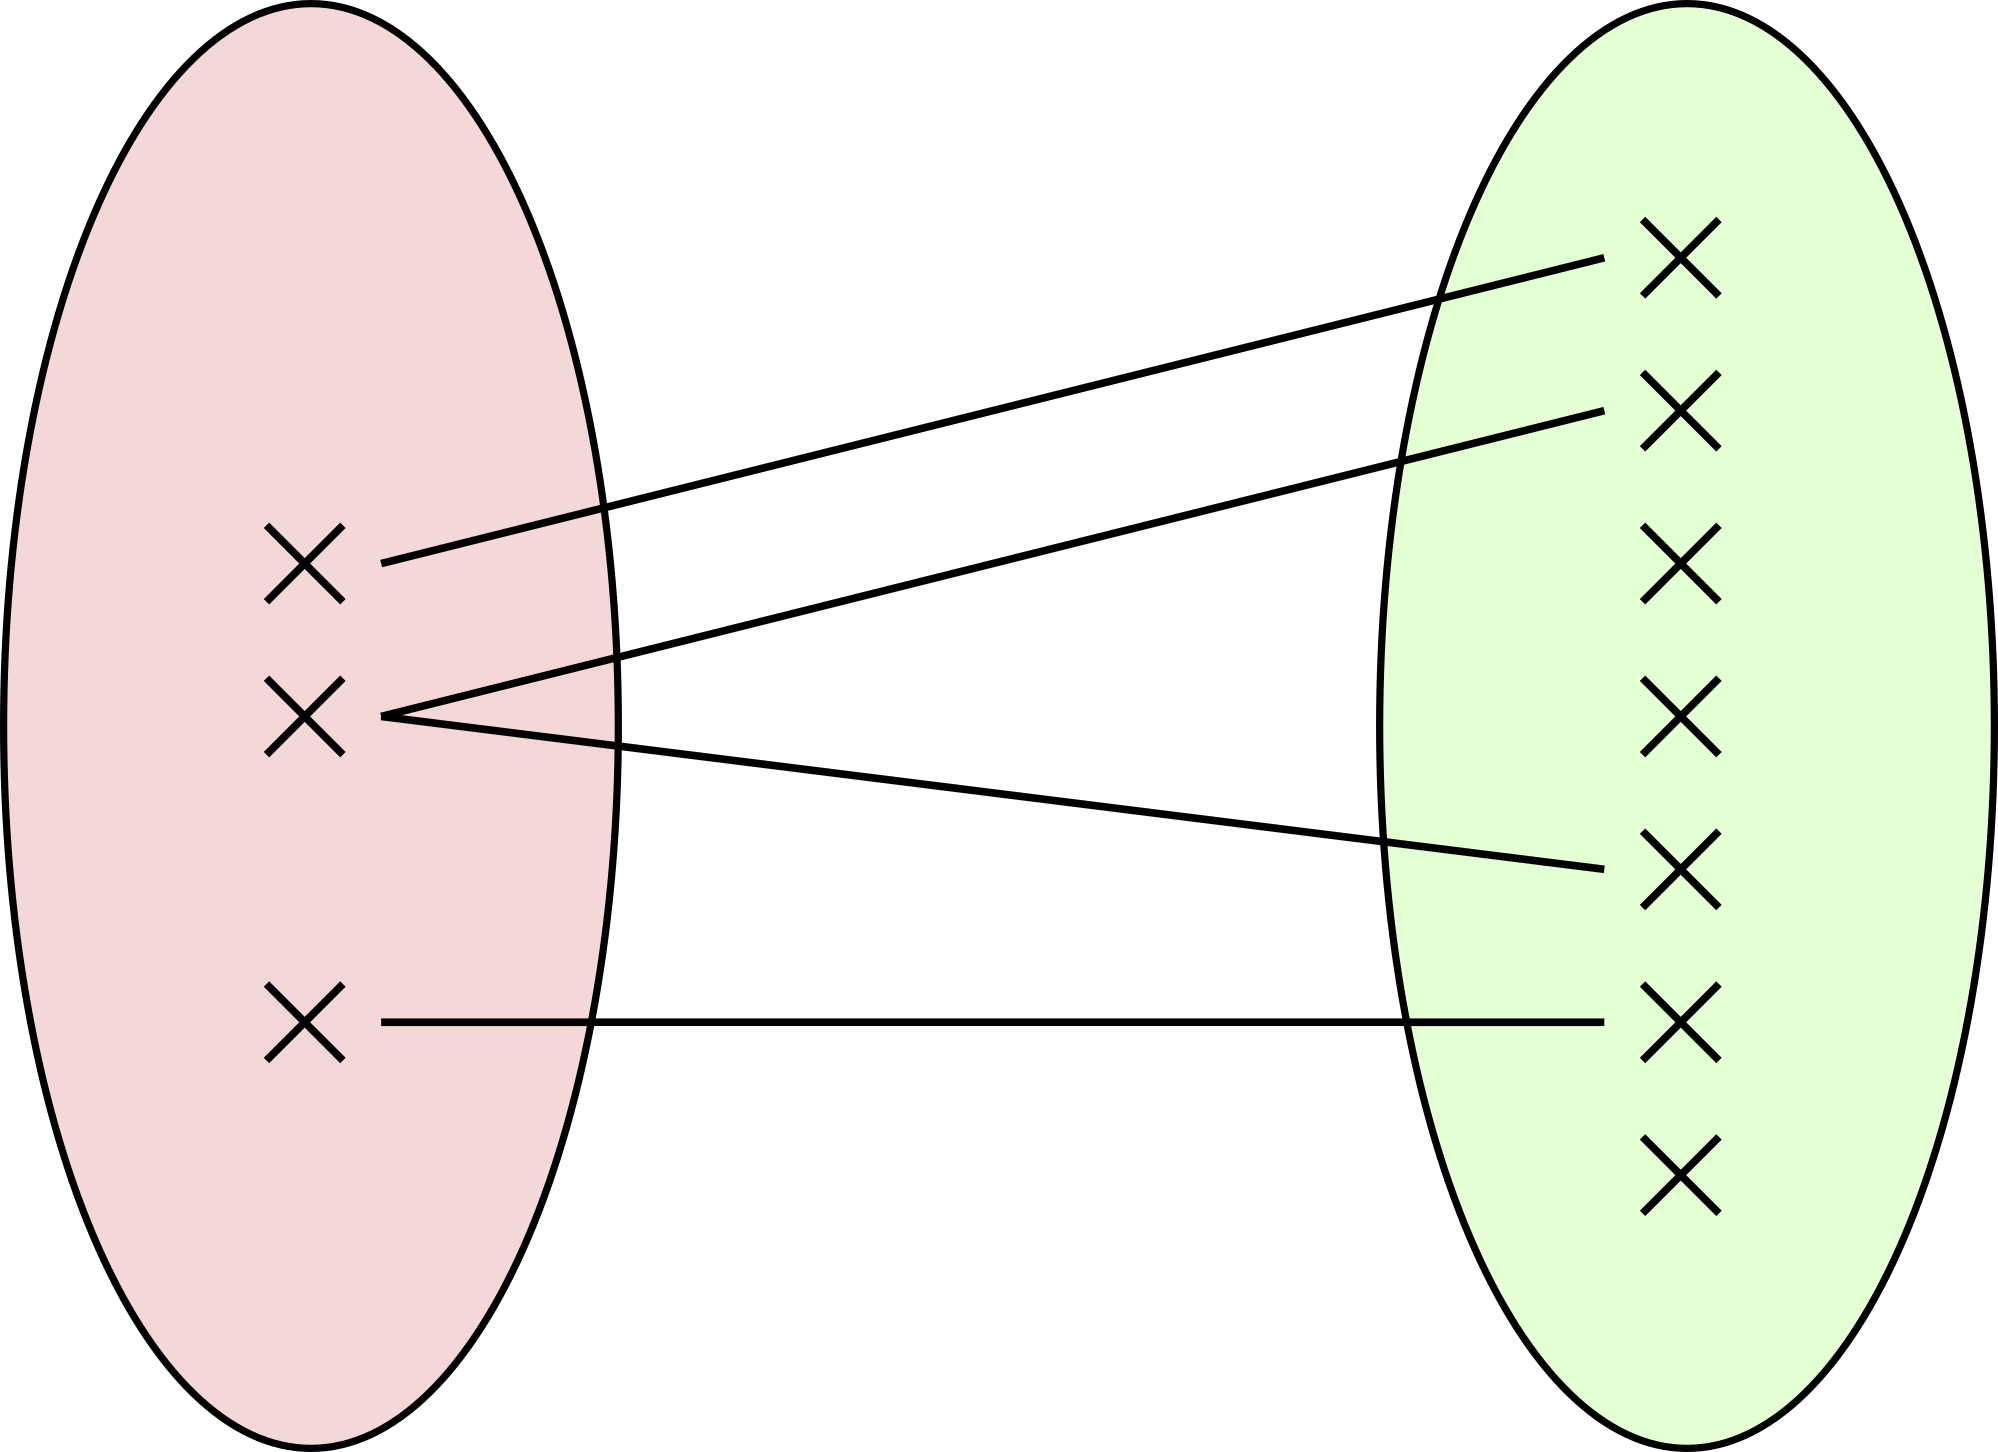
\includegraphics[width=\myw]{ensembles/img/3.png}
            \item 	\ \\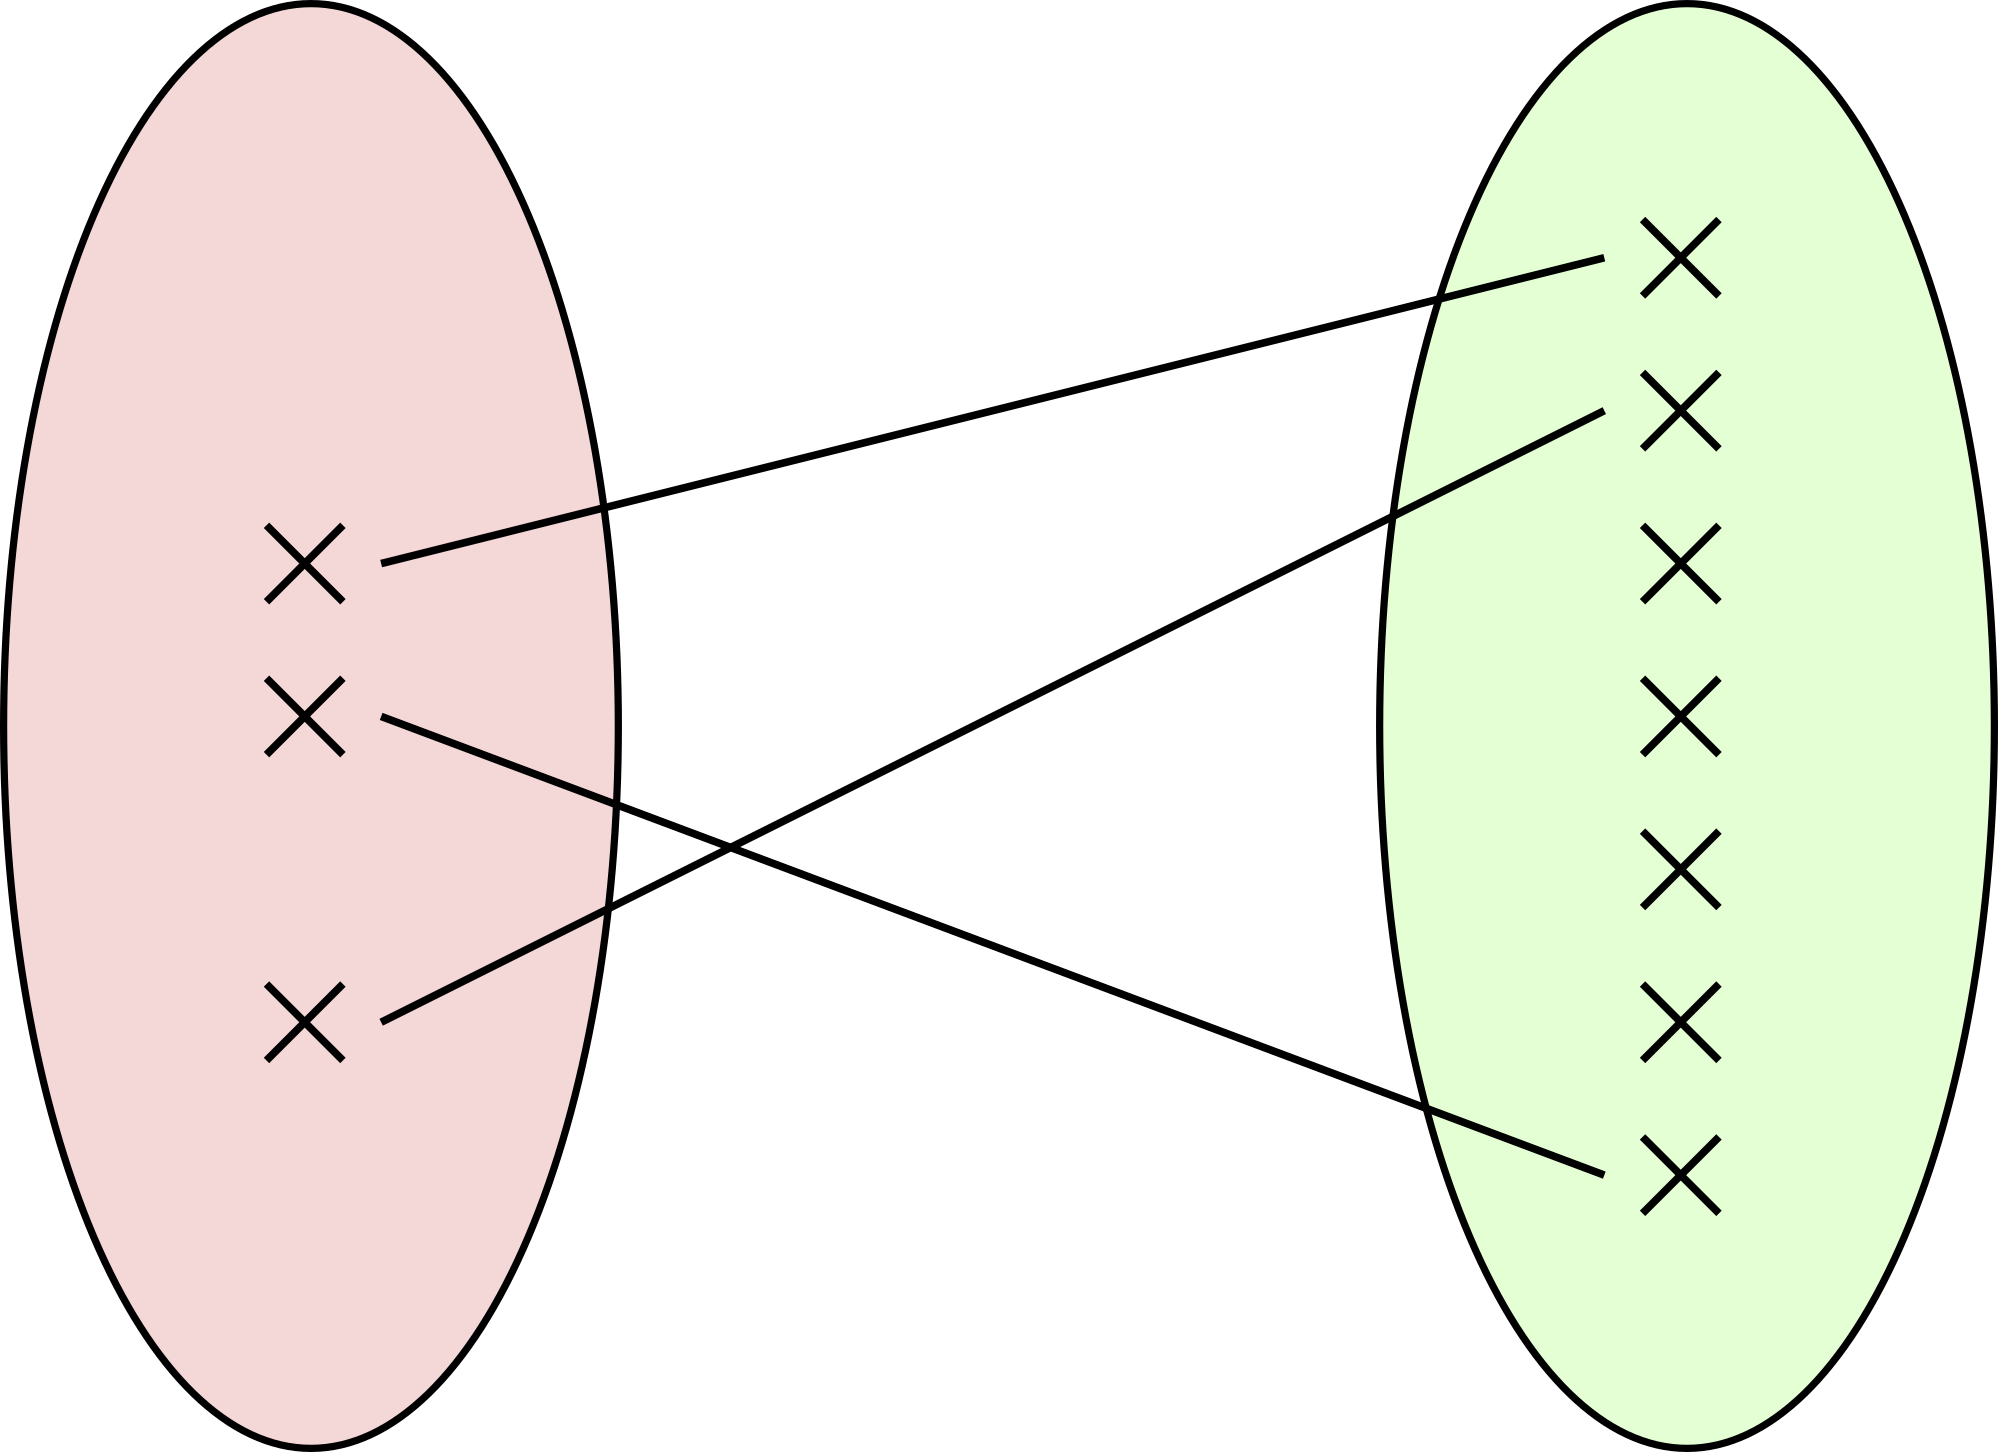
\includegraphics[width=\myw]{ensembles/img/4.png}
            \item 	\ \\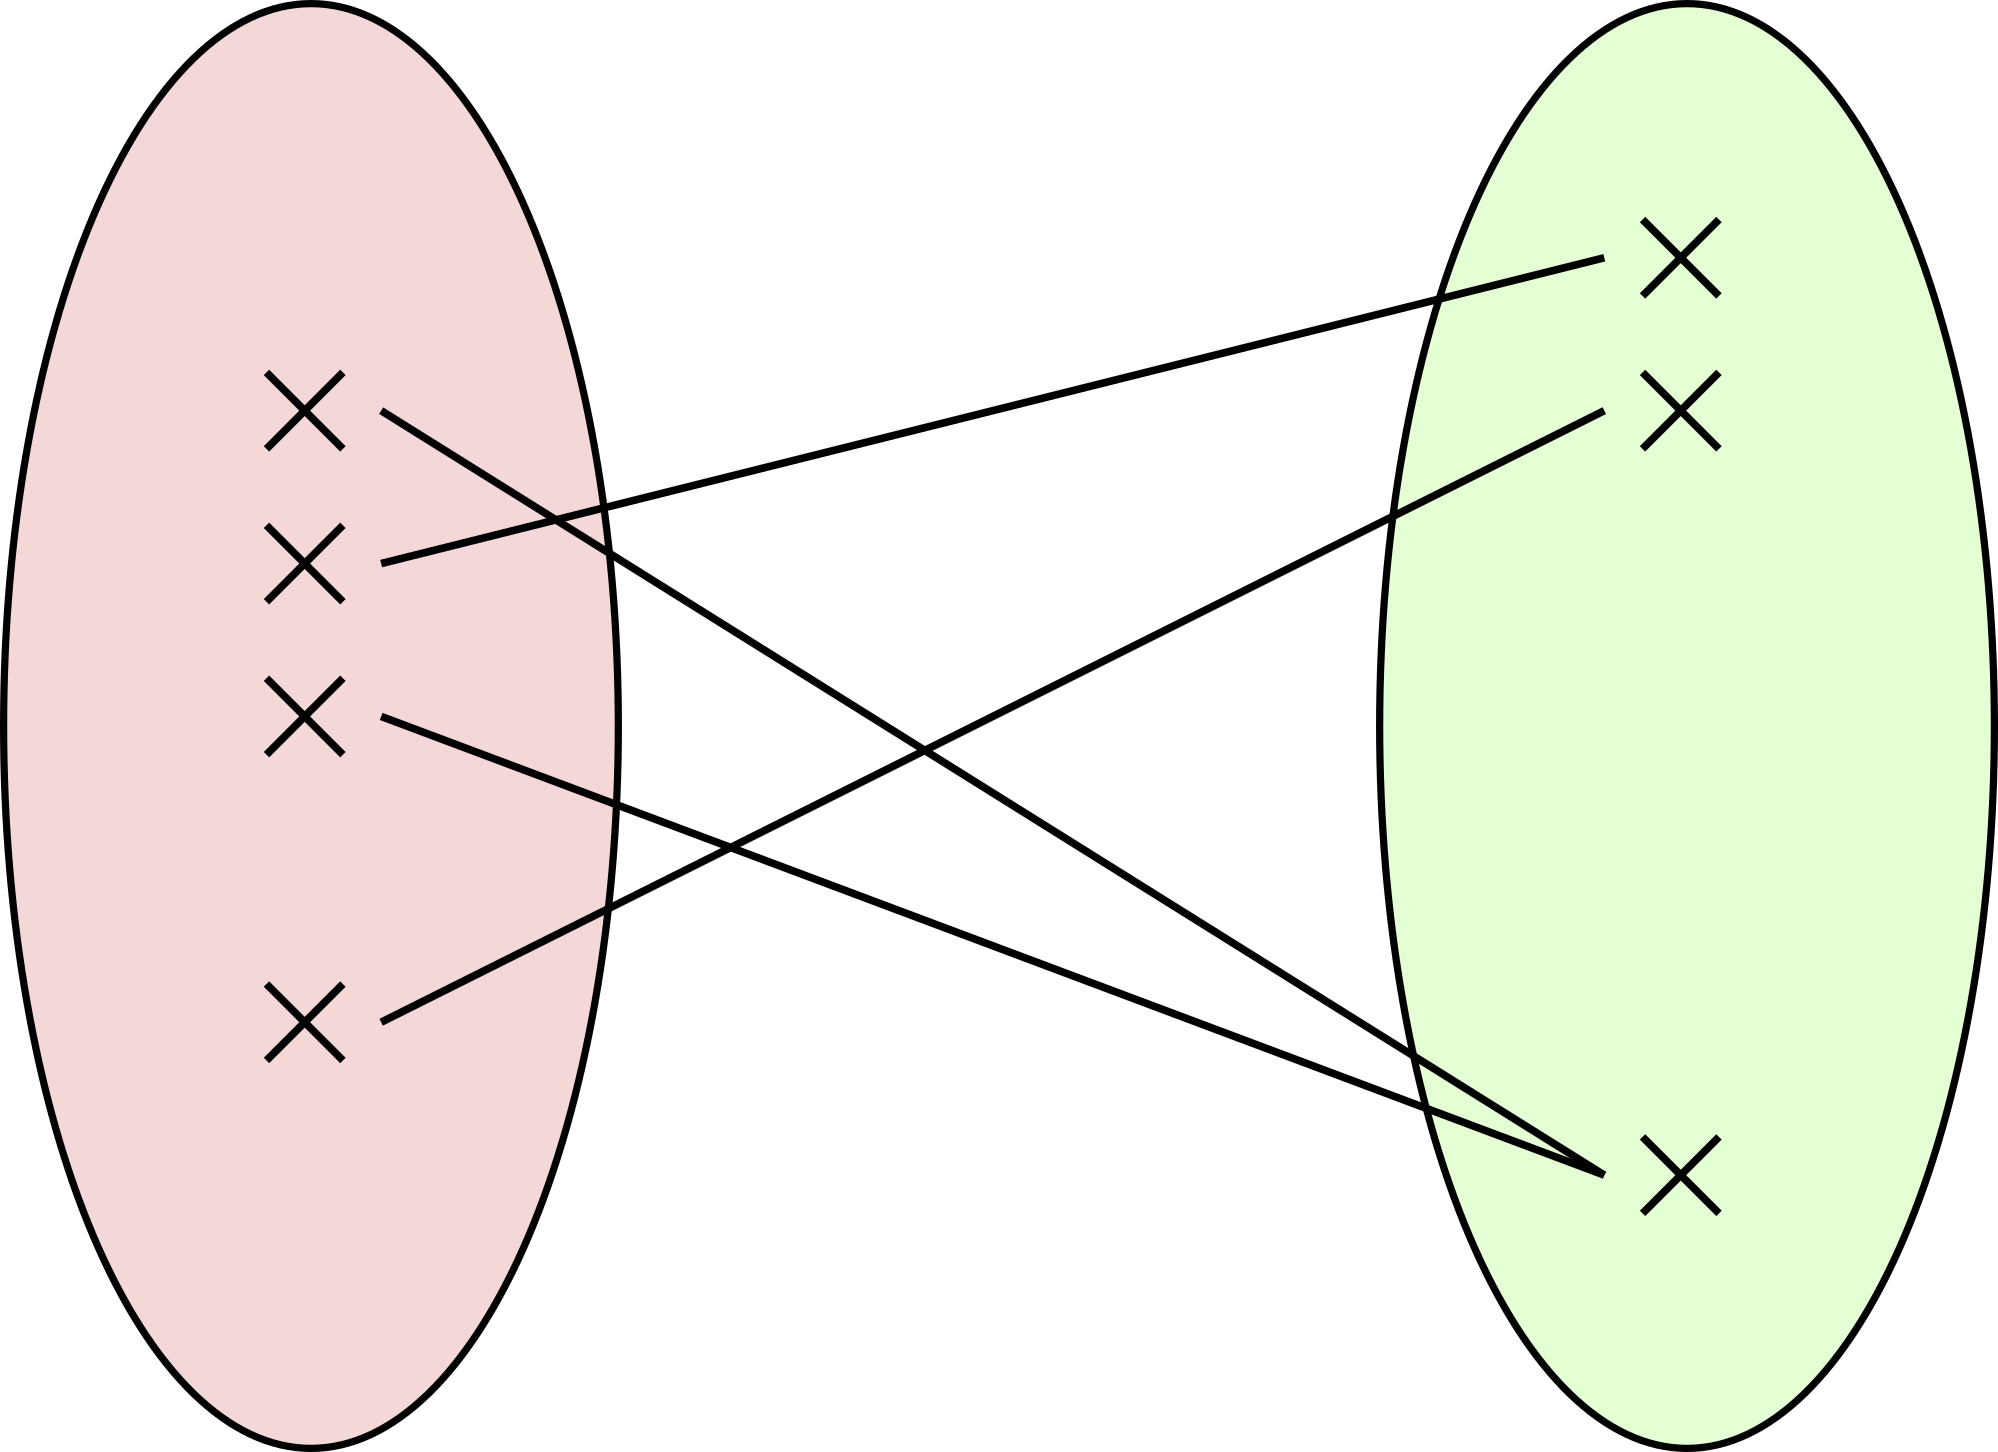
\includegraphics[width=\myw]{ensembles/img/5.png}
            \item 	\ \\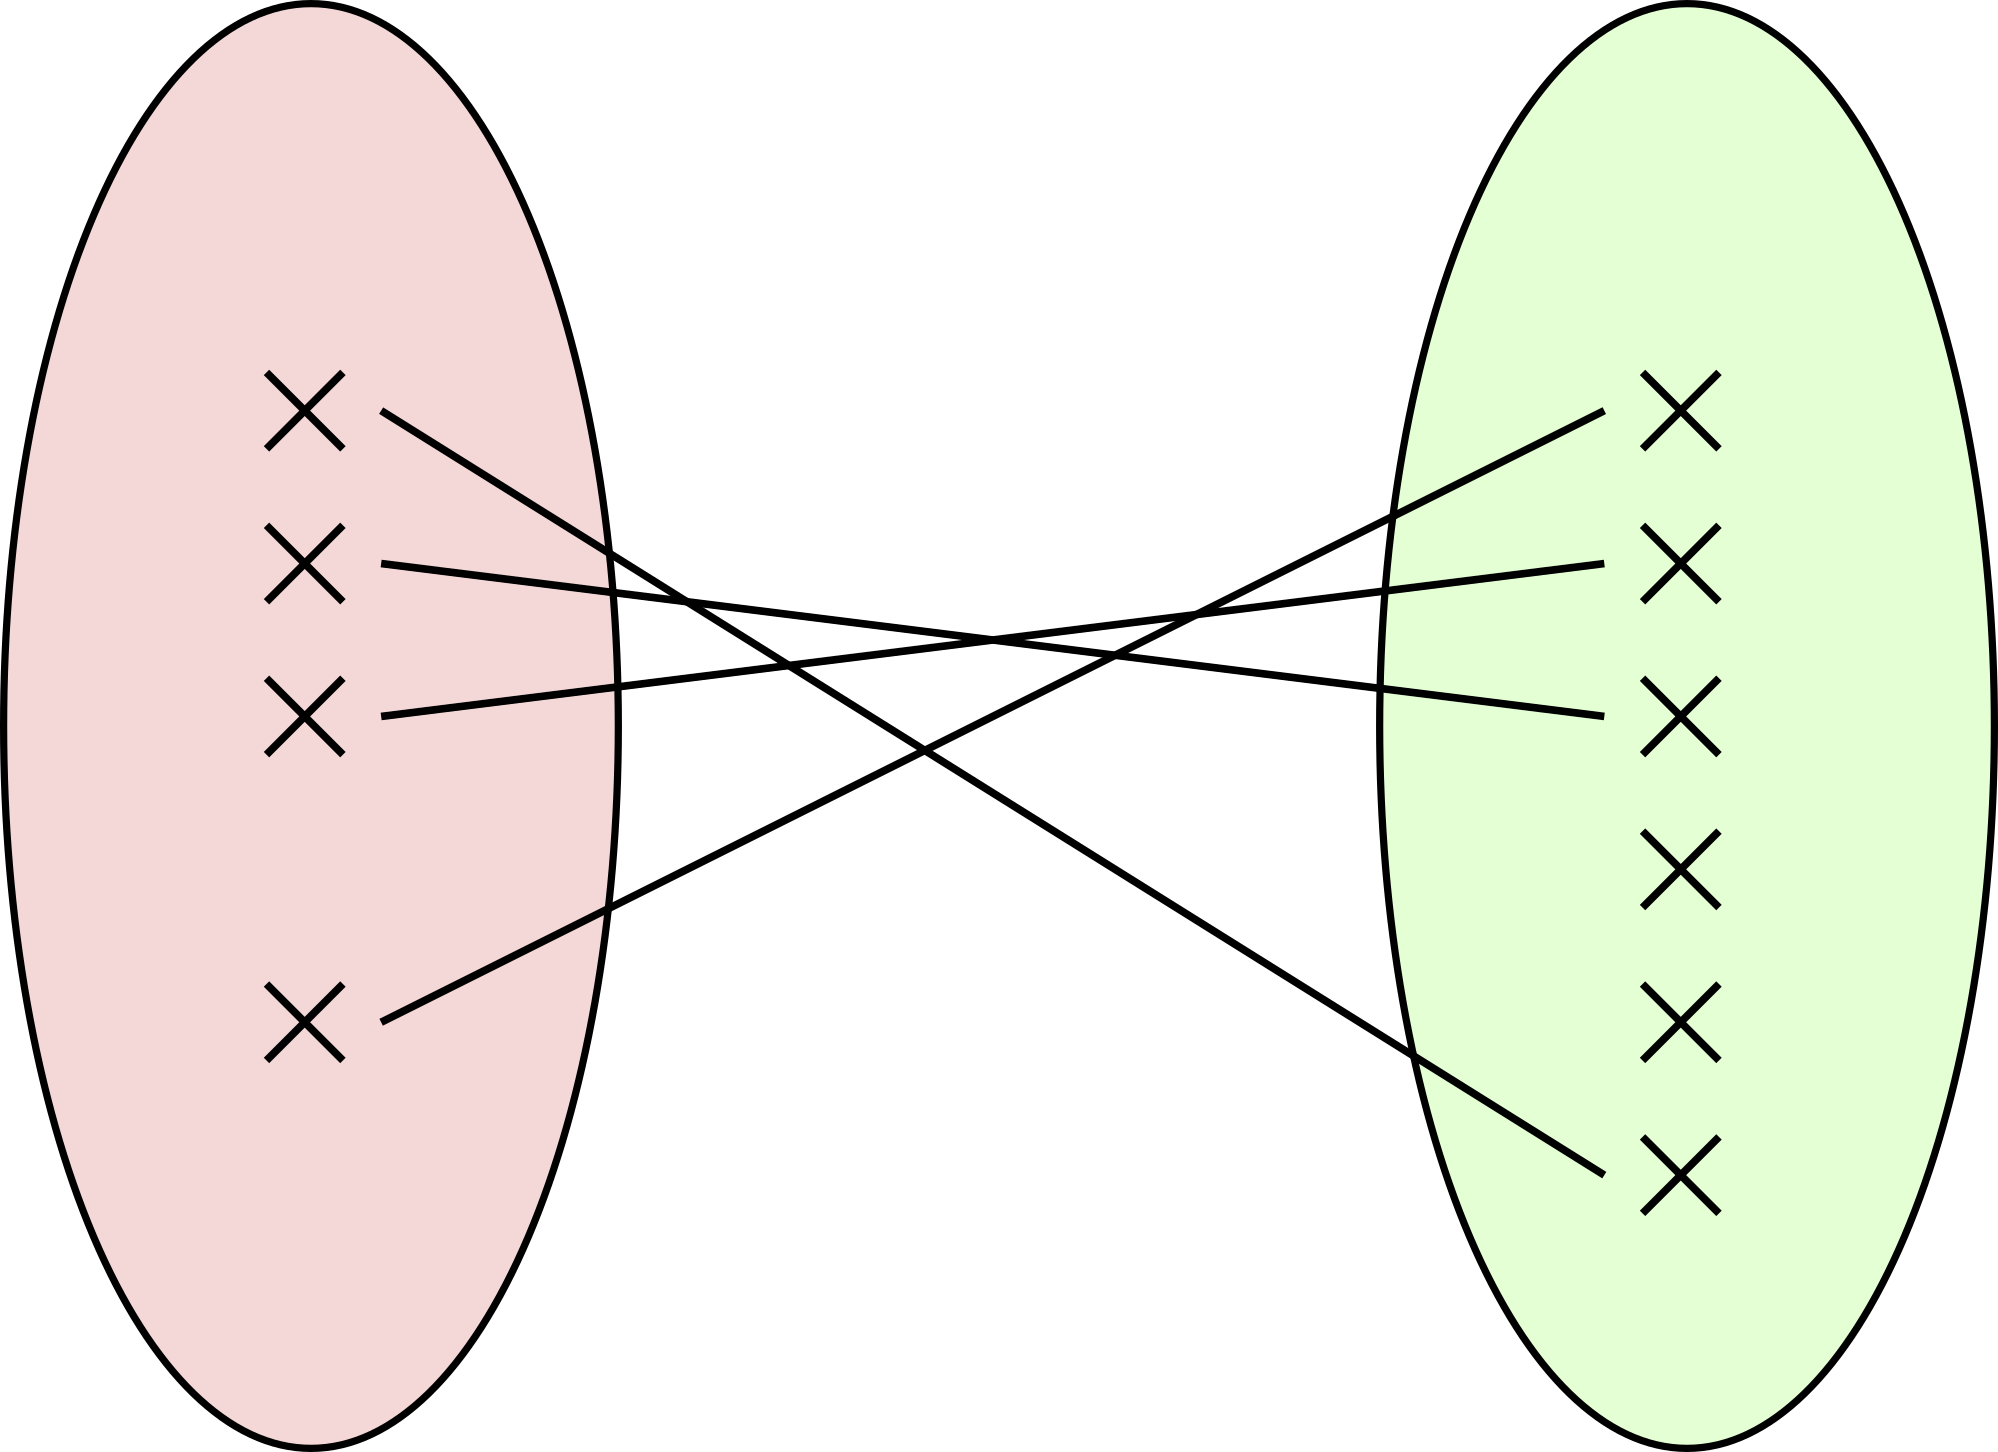
\includegraphics[width=\myw]{ensembles/img/6.png}
            \item 	\ \\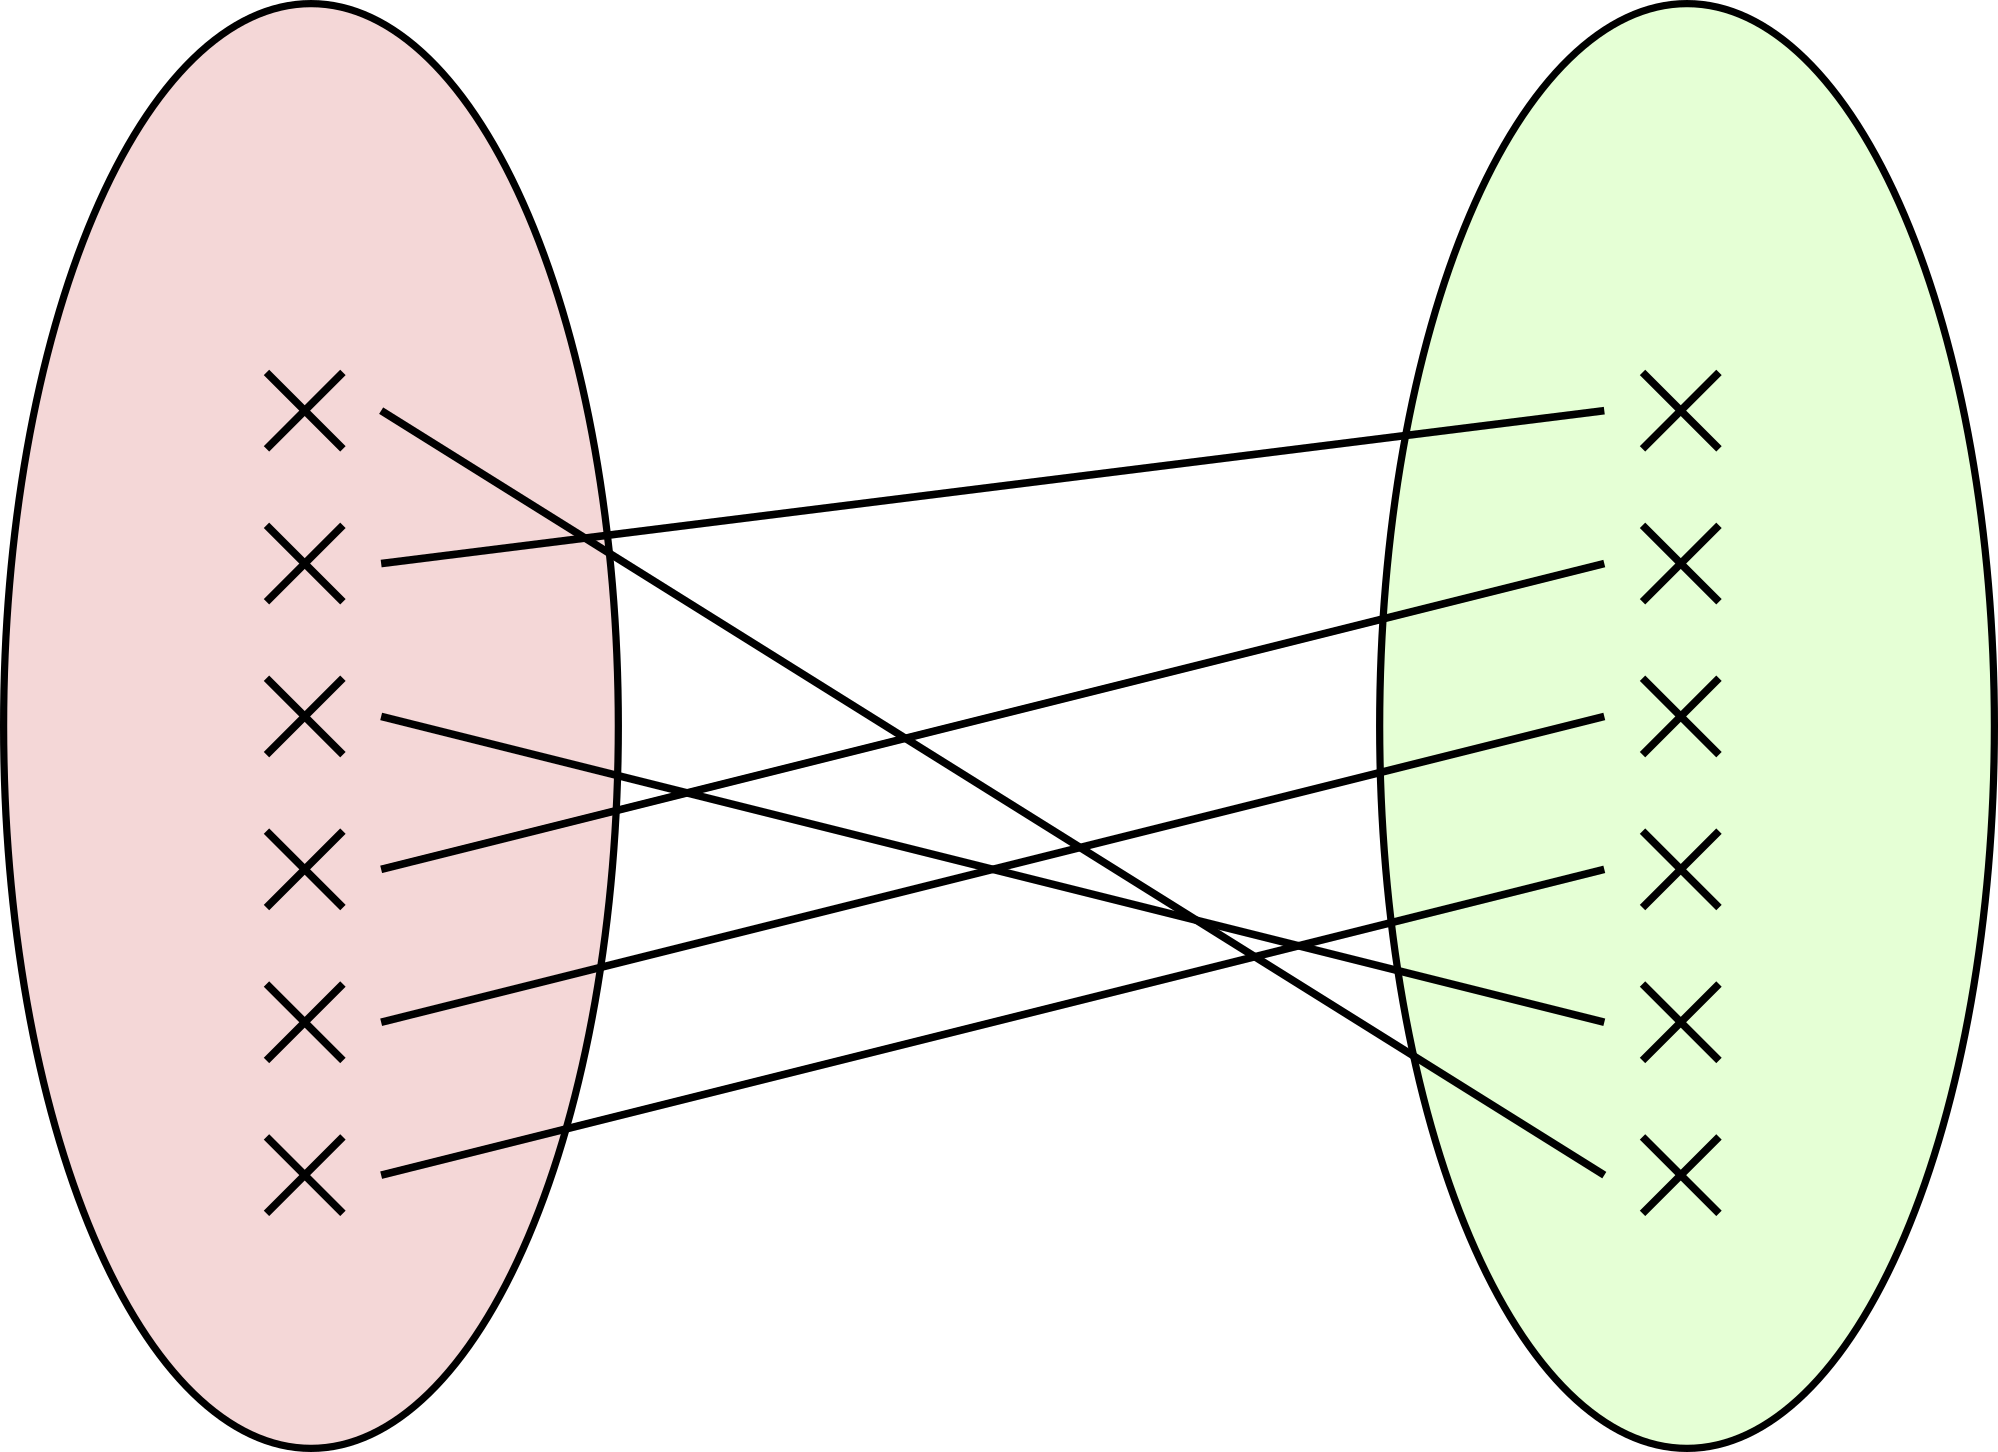
\includegraphics[width=\myw]{ensembles/img/7.png}
            \item 	\ \\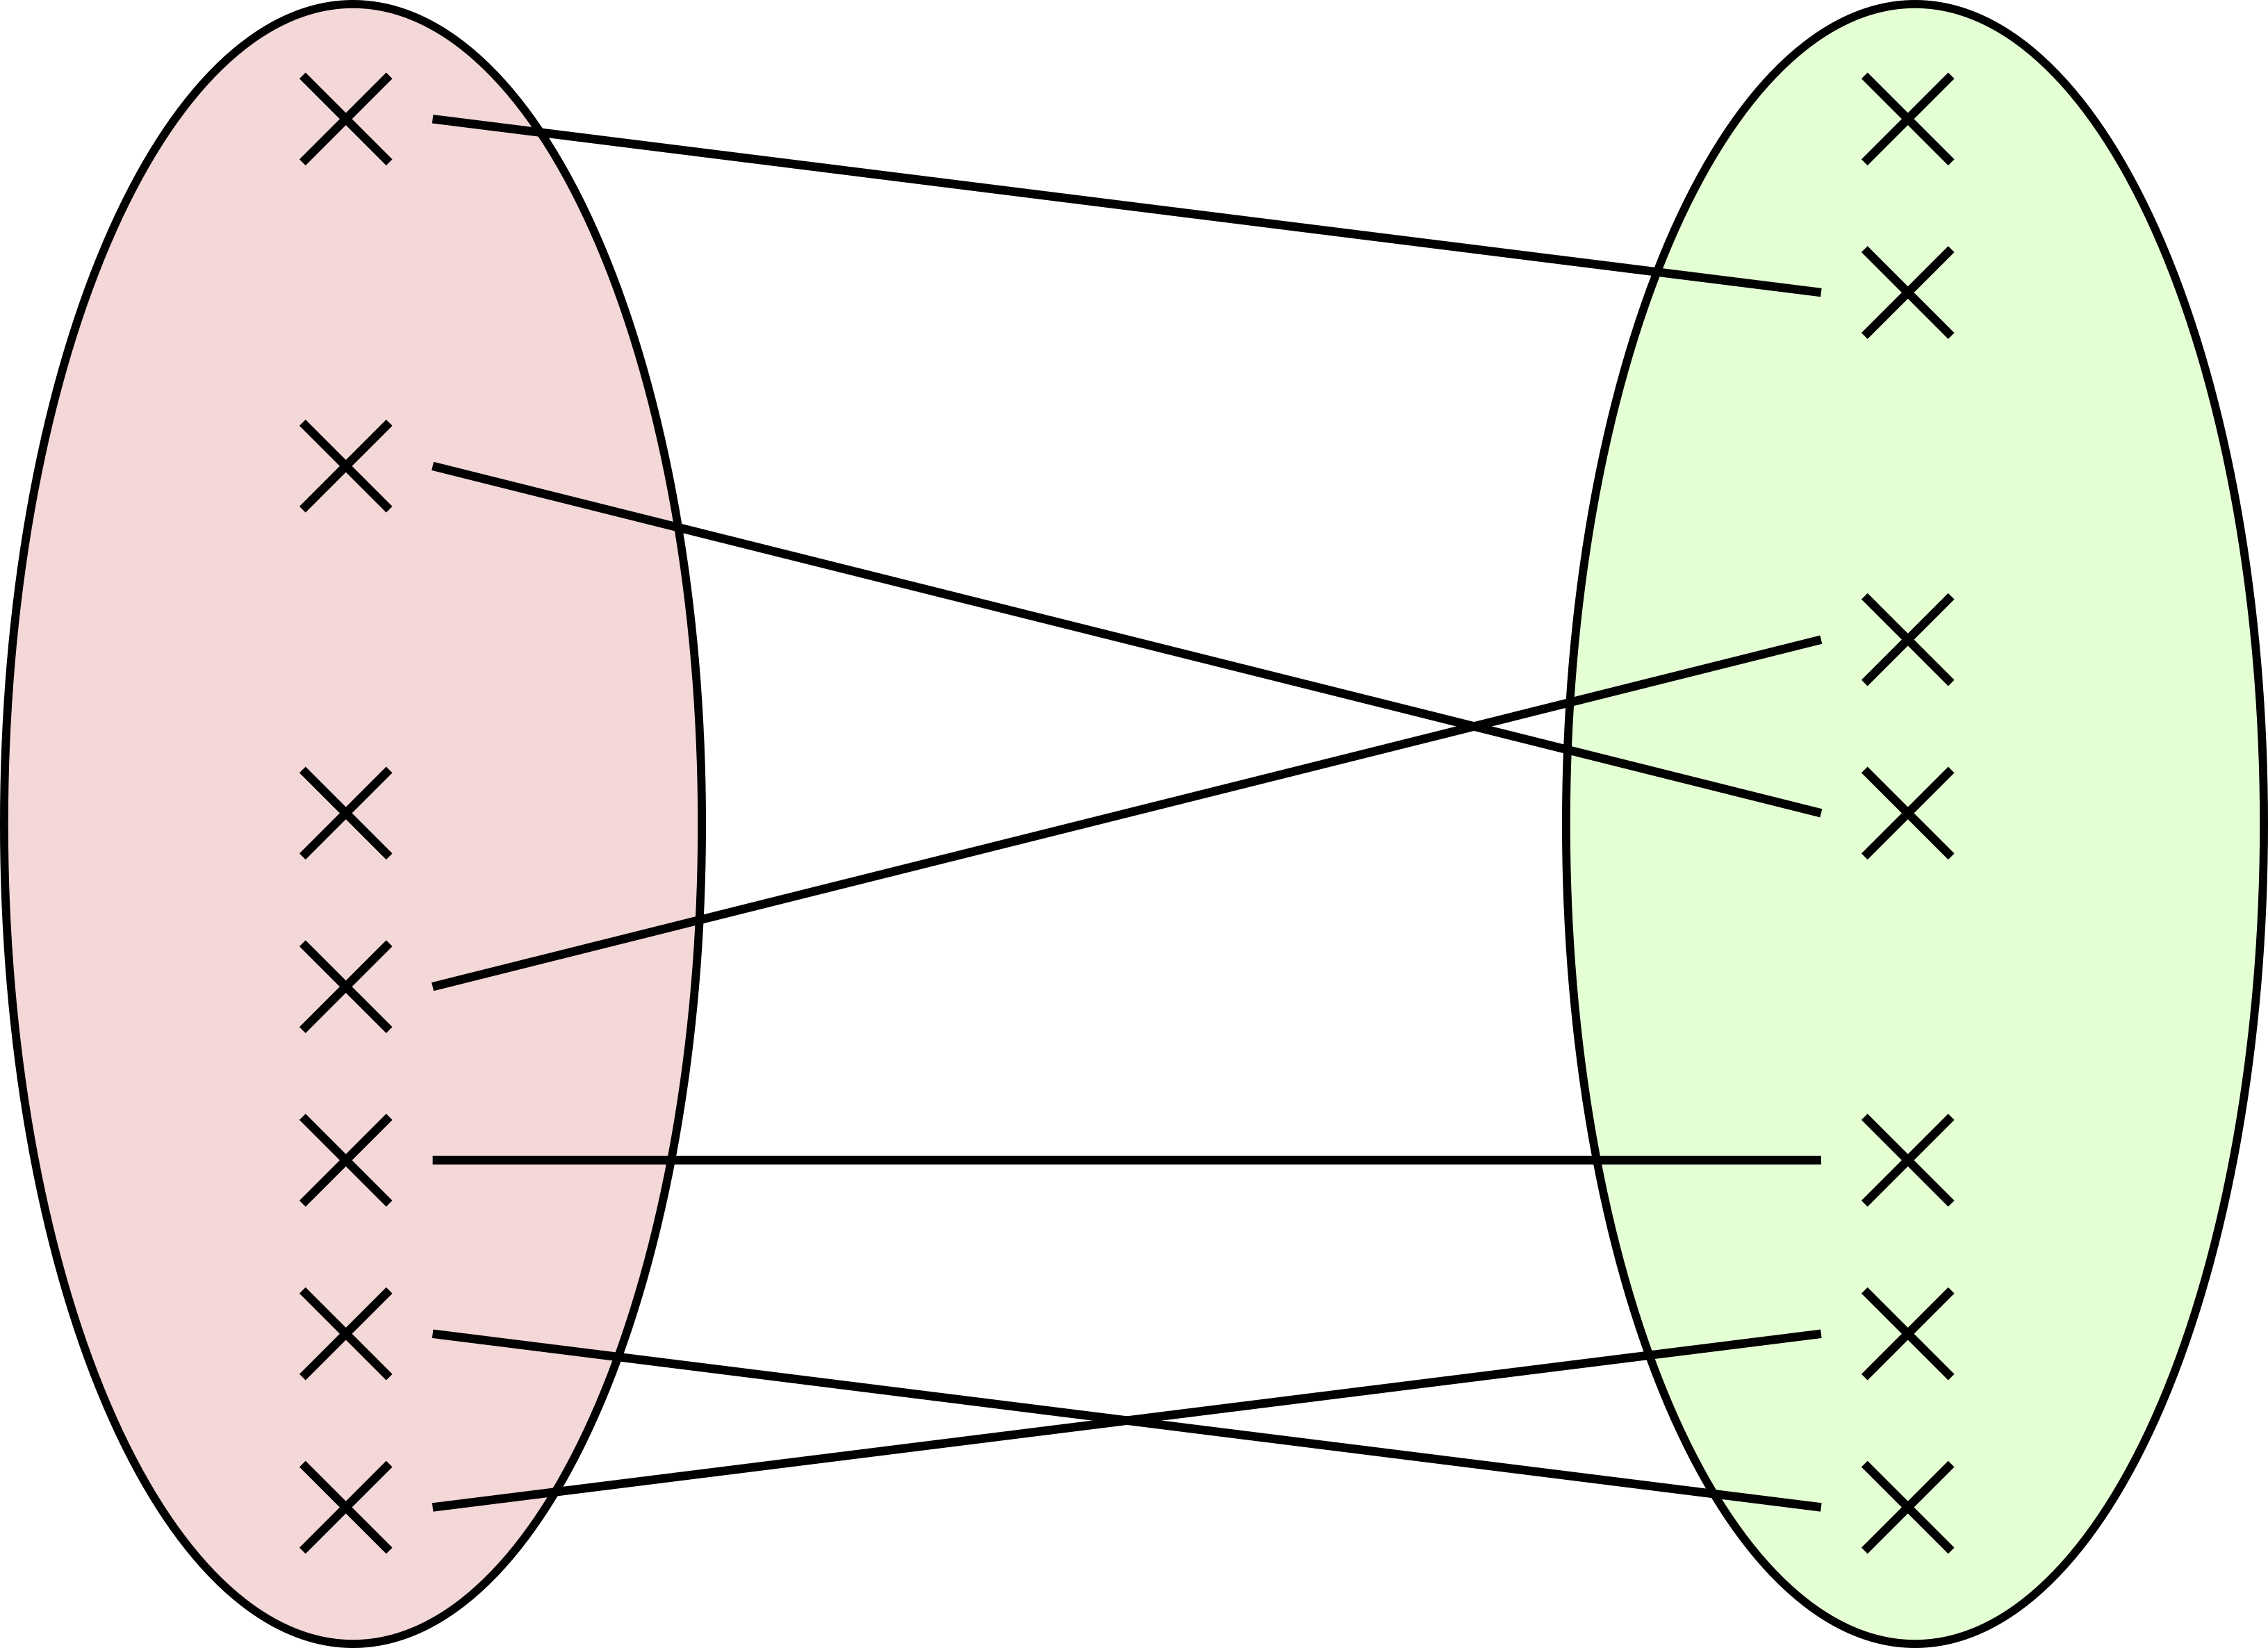
\includegraphics[width=\myw]{ensembles/img/8.png}
        \end{enumerate}    
    \end{multicols}
    
\end{exercice}

\begin{propriete}[ : bijection réciproque]
    Lorsque $f$ est une bijection de $E$ dans $F$, il est possible de construire sa \textit{bijection réciproque}. On la note $f^{-1}$, elle part de $F$, arrive dans $E$ et à tout élément $y$ de $F$ elle associe \textit{son unique antécédent} par $f$.
    \begin{center}
        \begin{tabbing}
            $f^{-1}\,:\,$ \=	$F\longrightarrow E$\\
            \>	$y \longmapsto x$\ \ où $x$ est l'unique élément de $E$ tel que $f(x)=y$.
        \end{tabbing}
    \end{center}
    Et on écrit que $x=f^{-1}(y)$.\\
\end{propriete}

\begin{exemple}[]
    $f$ est une bijection de $E$ dans $F$ : chaque élément de $F$ possède \textit{un unique} antécédent par $f$.\\
    Cela permet de construire la \textit{bijection réciproque} de $f$, notée $f^{-1}$. Celle-ci va de $F$ vers $E$. Puisque $f(e)=r$, on pose alors $f^{-1}(r)=e$, \textit{et c\ae tera}.\\
    \begin{center}
    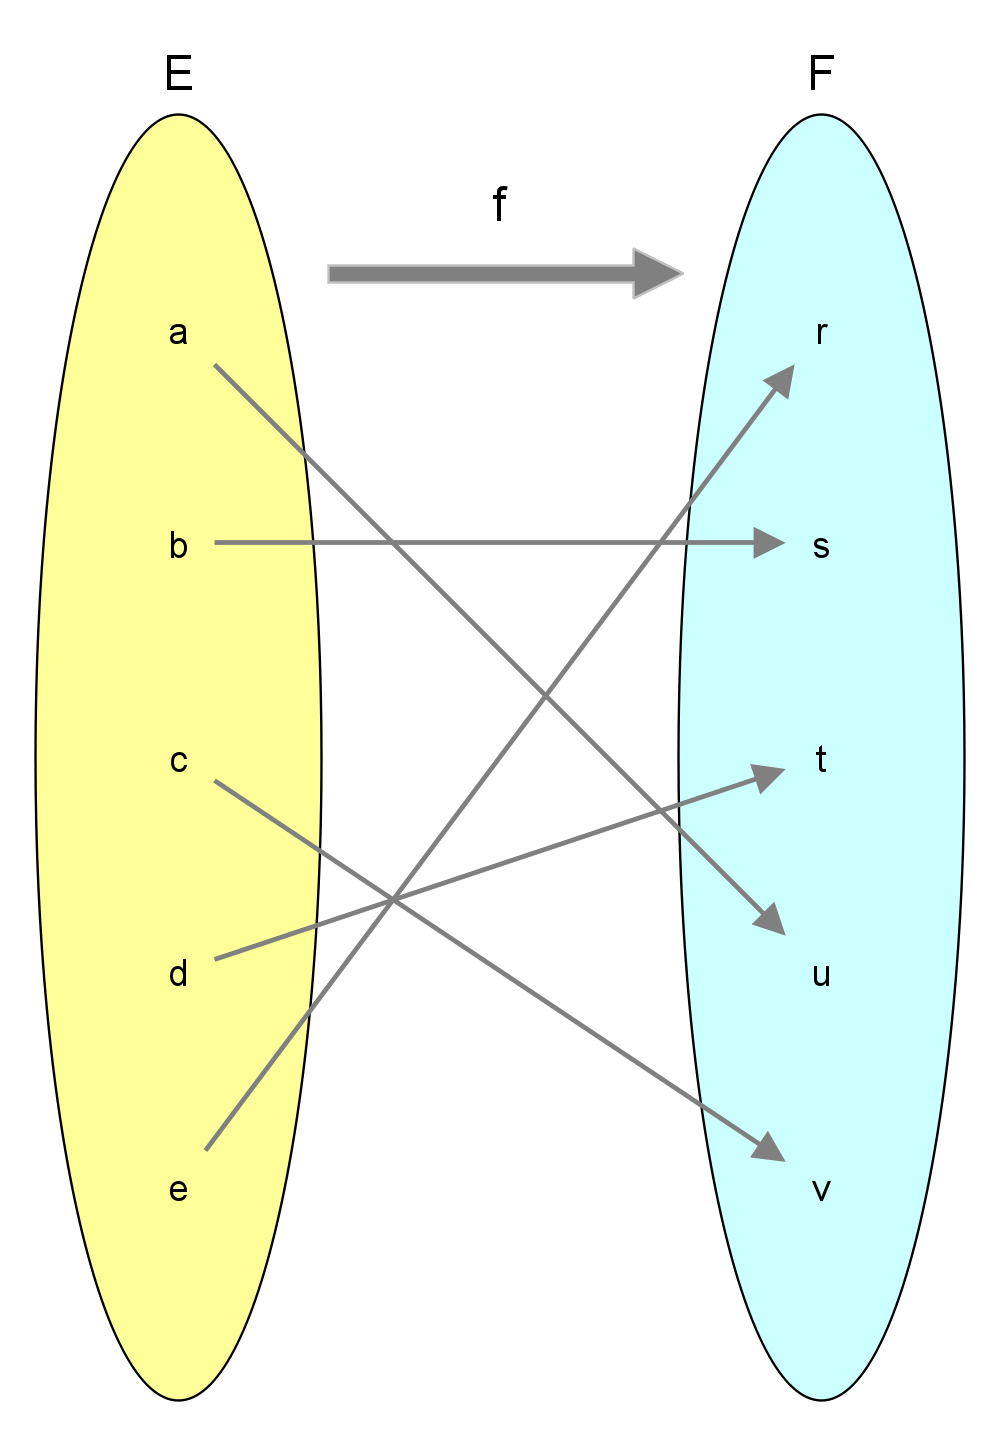
\includegraphics[width=5cm]{ensembles/img/bij.png}\hspace{4em}
    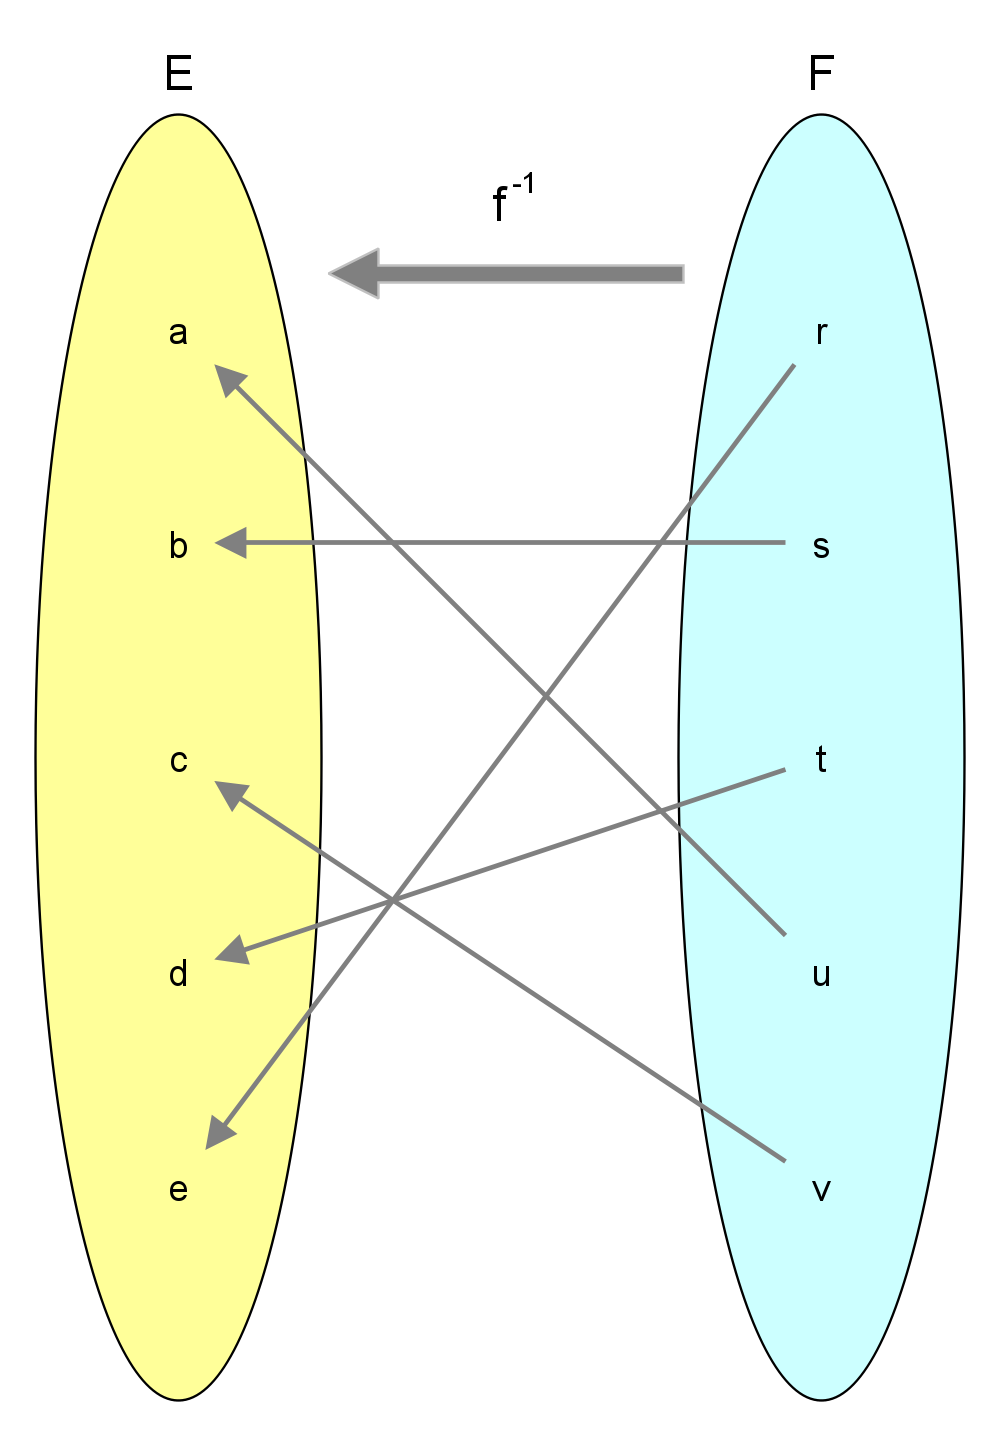
\includegraphics[width=5cm]{ensembles/img/bij_rec.png}
    \end{center}
    Il va sans dire que $f^{-1}$ est également une bijection.
\end{exemple}

\section{Extension aux parties d'une application}

\begin{definition}[ : image directe]
    Soit $f$ une application de $E$ dans $F$ et $A$ une partie de $E$. On appelle \textit{image directe de $A$ par $f$} et on note $f(A)$ la partie de $F$ constituée des images des éléments de $A$ par $f$.
    $$f(A)=\left\lbrace f(x)\::\:x\in A\right\rbrace$$
\end{definition}

\begin{exemple}[]
    $A$ est la partie de $E$ constituée de $a$, $b$, $c$.\\
    On considère $B$, partie de $F$ constituée de $f(a)=s$, $f(b)=r$ et $f(c)=s$ (élément déjà atteint par $a$).$$B=f(A)$$
    \begin{center}
        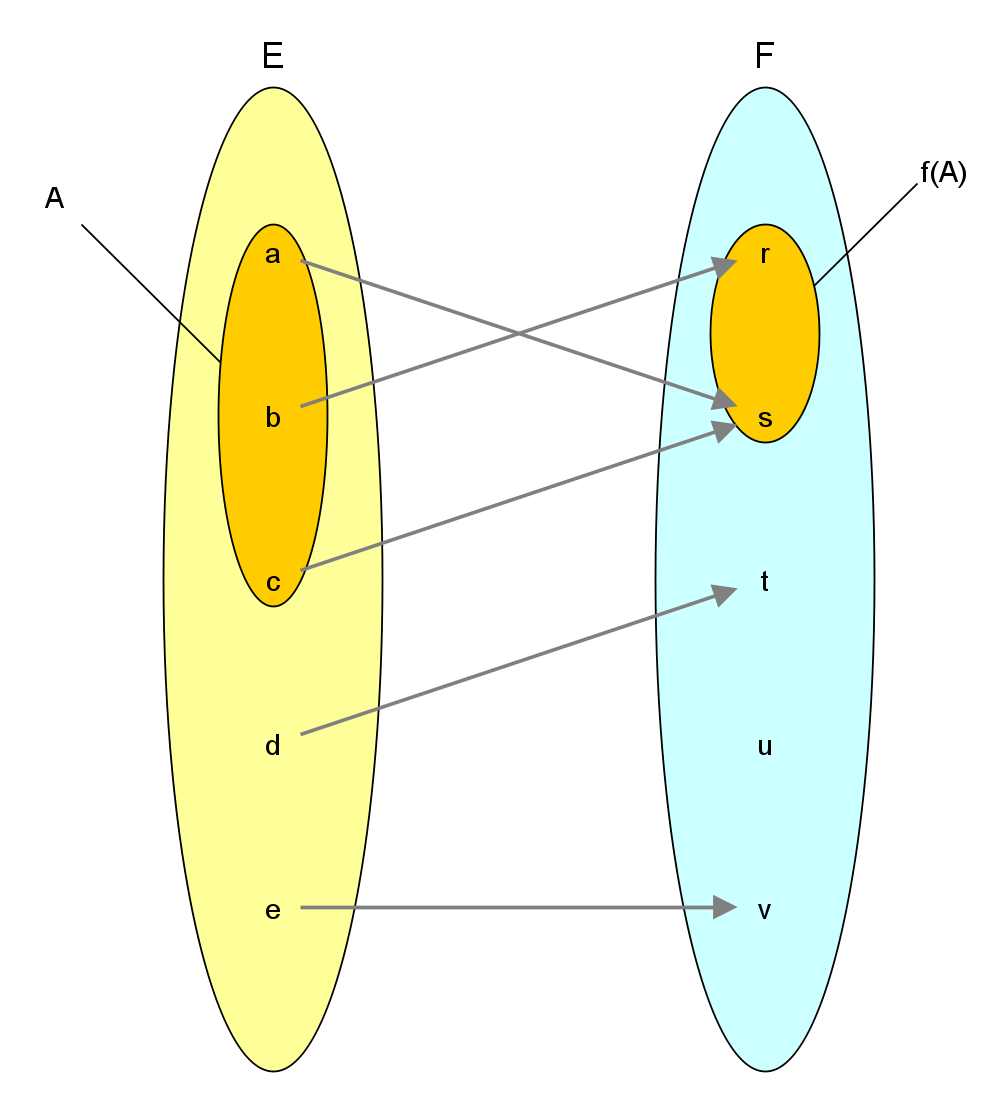
\includegraphics[width=5cm]{ensembles/img/im_dir.png}
    \end{center}
\end{exemple}

\begin{definition}[ : image réciproque]
    Soit $f$ une application de $E$ dans $F$ et $B$ une partie de $F$. On appelle \textit{image réciproque de $B$ par $f$} et on note $f^{-1}(B)$ la partie de $E$ constituée des \textit{antécédents} des éléments de $B$ par $f$.
    $$f^{-1}(B)=\left\lbrace x\in E\::\:f(x)\in B\right\rbrace$$
\end{definition}

\begin{exemple}[]
    \begin{center}
        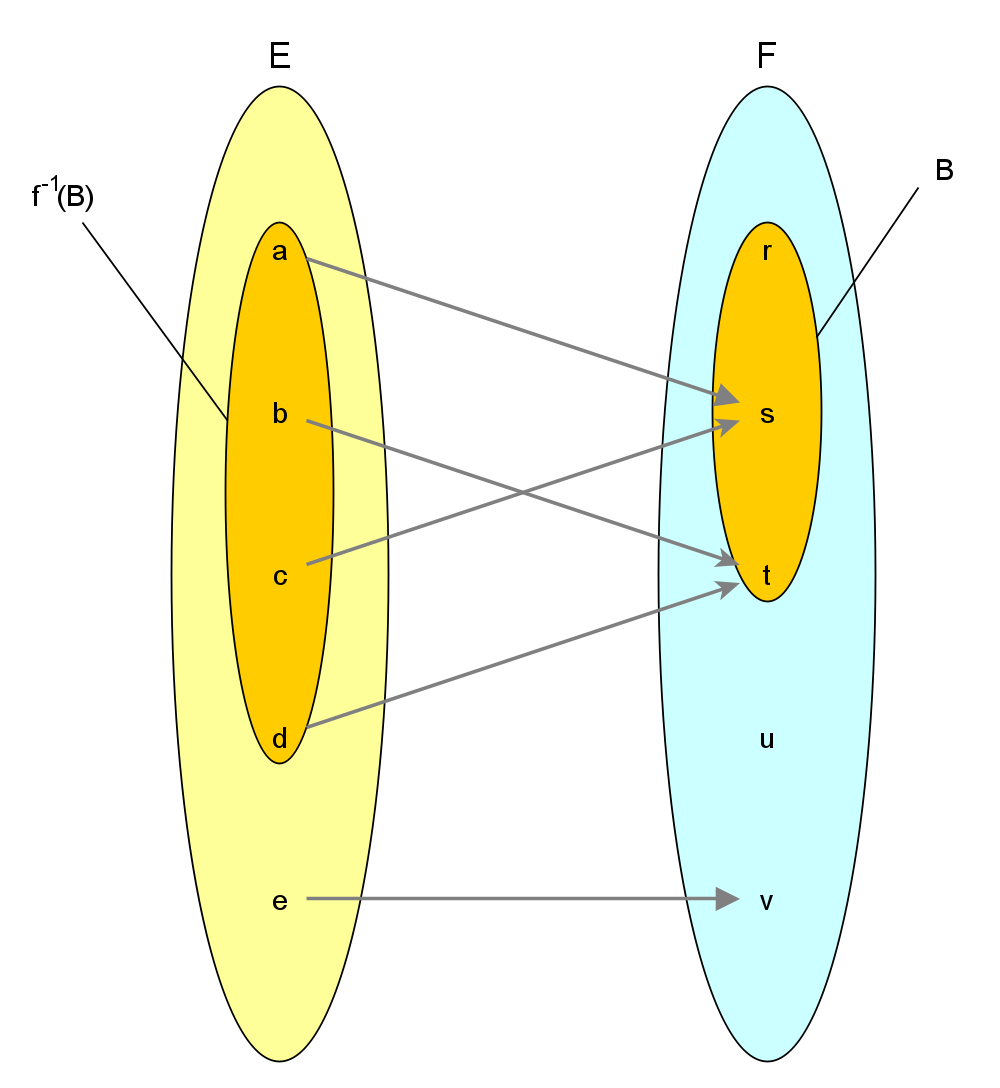
\includegraphics[width=5cm]{ensembles/img/im_rec.png}
    \end{center}
    $B$ est la partie de $F$ constituée de $r$, $s$, $t$.\\
    $r$ n'a pas d'antécédent par $f$, $s$ en a deux : $a$ et $c$, et $t$ en a également 2 : $b$ et $d$.\\
    $$f^{-1}(B)=\left\lbrace a;\,b;\,c;\,d\right\rbrace$$
\end{exemple}

\begin{remarque}[]
    La notation $f^{-1}$ est trompeuse : $f$ n'est pas obligatoirement bijective, donc l'\textit{application} $f^{-1}$ n'est pas obligatoirement définie. Ceci dit il est possible de déterminer $f^{-1}(B)$ quand $B$ est une \textit{partie} de F même si $f$ n'est pas bijective.
\end{remarque}

\begin{exercice}[]
    $E=\lbrace 0;1;2;3;4;5;6;7\rbrace$ et $F=\lbrace 0;1;2;3\rbrace$.\\
    $f$ est l'application de $E$ dans $F$ qui à tout élément de $E$ associe son reste dans la division euclidienne par 3.
    \begin{enumerate}
        \item 	$f$ est-elle injective ? Surjective ?
        \item 	Posons $A=\lbrace 1;3;4\rbrace$, déterminer $f(A)$, puis posant $B=f(A)$, déterminer $f^{-1}(B)$.
        \item 	Posons $C=\lbrace 2;3\rbrace$, déterminer $f^{-1}(C)$, puis, en posant $D=f^{-1}(C)$, déterminer $f(D)$.\\
    \end{enumerate}
\end{exercice}


\begin{exercice}[]
    Soit $f$ l'application de $\R$. dans $\R$. définie par $f(x) = 4x + 10$.
    \begin{enumerate}
        \item 	f est-elle une injection ?
        \item 	f est-elle une surjection ?
        \item 	f est-elle une bijection ?
        \item 	Déterminer l'image directe de $\fif{2}{3}$ et de $\fii{0}$.
        \item 	Déterminer l'image réciproque de $\fii{0}$.\\
    \end{enumerate}
\end{exercice}


\section{Composition}

\begin{definition}[ : composée de deux applications]
    Soit $f$ une application de $E$ dans $F$ et $g$ une application de $F$ dans $G$.\\
    Alors on définit la \textit{composée} de $g$ par $f$ et on note $g\circ f$ l'application de $E$ dans $G$ définie par
    $$g\circ f (x)= g\left(f(x)\right)$$
\end{definition}

\begin{exemple}[]
    Les applications $f$ et $g$ sont décrites par le diagramme ci-contre.\\
    L'application $g\circ f$ est donc définie de $E$ dans $G$ et
    \begin{itemize}
        \item 	$g\circ f(a)=2$
        \item 	$g\circ f(b)=1$
        \item 	$g\circ f(c)=2$
        \item 	$g\circ f(d)=1$
        \item 	$g\circ f(e)=4$
    \end{itemize}
    \begin{center}
        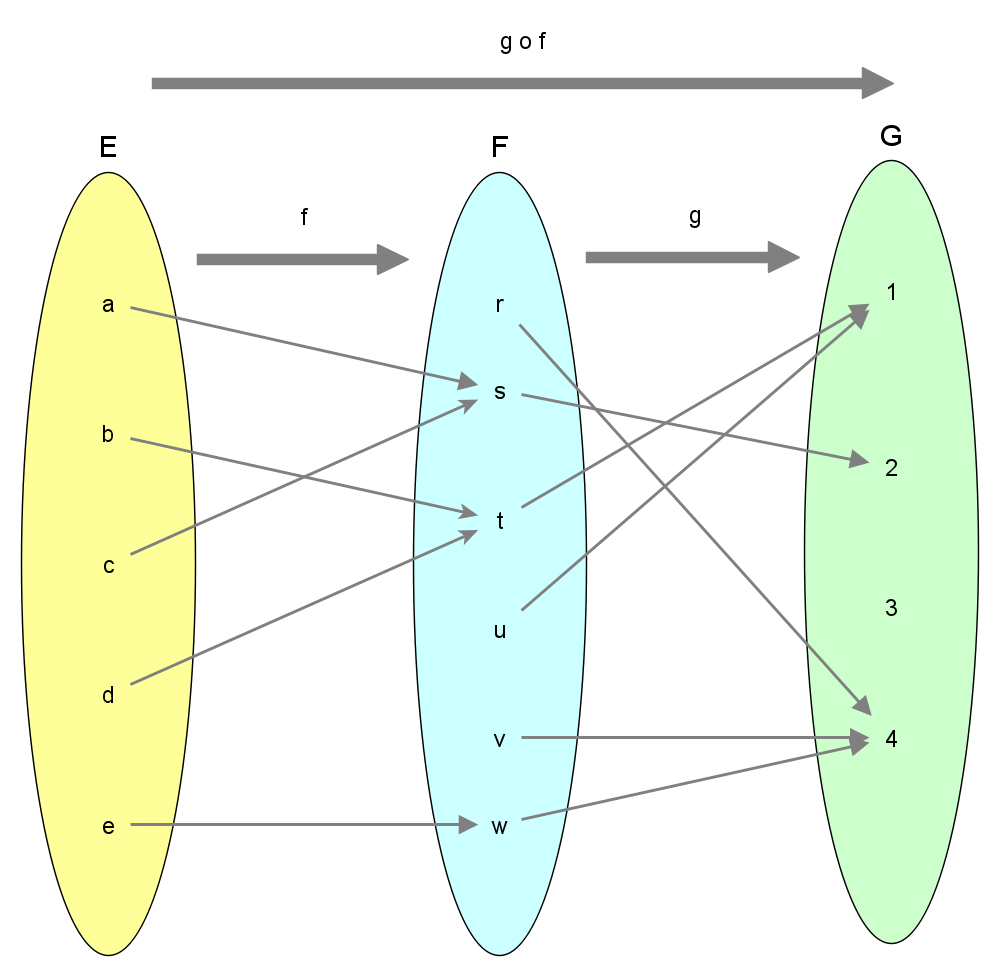
\includegraphics[width=7cm]{ensembles/img/compo.png}
    \end{center}
\end{exemple}

\begin{exercice}[]
    $E=\lbrace a;b;c;d\rbrace$, $F=\lbrace 1;2;3\rbrace$ et $G\lbrace \alpha;\beta;\gamma\rbrace$.\\
    $f$ est définie de $E$ dans $F$  et $g$ de $F$ dans $G$ par\\
    $f(a)=2$, $f(b)=1$, $f(c)=3$ et $g(1)=\gamma$, $g(2)=\alpha$ et $g(3)=\beta$.
    \begin{enumerate}
        \item 	$f$ et $g$ sont-elles injectives ? Surjectives ? Bijectives ?
        \item 	Définir l'application $g\circ f$.
        \item 	Peut-on définir l'application réciproque de $f$ ? De $g$ ?
    \end{enumerate}
\end{exercice}

\begin{exercice}[*]
    Expliciter  $f\circ g$ et $g\circ f$ lorsque $f$ et $g$
    sont les fonctions suivantes :
    \begin{multicols}{2}
        \begin{tabbing}
            $f\ :\ $	\=	$\R$	\=	$\longrightarrow$	\=	$\oii{0}$\\
            \>	$x$		\> 	$\longmapsto$		\>	$x^2+2$
        \end{tabbing}
        \begin{tabbing}
            $g\ :\ $	\=	$\oii{0}$	\=	$\longrightarrow$	\=	$\R$\\
            \>	$x$		\> 	$\longmapsto$		\>	$\dfrac{1}{\sqrt{x}-1}$
        \end{tabbing}
    \end{multicols}
\end{exercice}

\begin{exercice}[]
    Un administrateur réseau gère le parc d'une petite entreprise qui comprend 9 ordinateurs. Chaque
    ordinateur possède une adresse de carte réseau, dite adresse MAC (Media Access Control) unique.\\
    L'administrateur a assigné une adresse IP (Internet Protocol) à chaque ordinateur à l'aide d'un
    logiciel installé sur le serveur. Il obtient le tableau suivant:
    \begin{center}
        \tabstyled
        \begin{tabular}{c|c|c}\hline
            
            \ccell Adresse MAC            & \ccell n° de poste & \ccell Adresse IP \\ \hline
            00~:~FF~:~B4~:~A9~:~96~:~11 & 1                       & 172.16.0.21     \\ \hline
            00~:~FF~:~B4~:~B0~:~45~:~1A & 2                       & 172.16.0.22     \\ \hline
            00~:~FF~:~B4~:~00~:~C5~:~DE & 3                       & 172.16.0.23     \\ \hline
            00~:~EE~:~B5~:~01~:~32~:~C4 & 4                       & 172.16.0.24     \\ \hline
            00~:~EE~:~B5~:~01~:~32~:~C5 & 5                       & 172.16.0.25     \\ \hline
            00~:~EE~:~B5~:~01~:~32~:~C6 & 6                       & 172.16.0.26     \\ \hline
            00~:~FF~:~B4~:~00~:~C5~:~DF & 7                       & 172.16.0.27     \\ \hline
            00~:~FF~:~B4~:~00~:~02~:~98 & 8                       & 172.16.0.28     \\ \hline
            00~:~EE~:~B5~:~01~:~34~:~CA & 9                       & 172.16.0.29     \\ \hline
        \end{tabular}
    \end{center}

    On considère l'application $f$ qui, à un numéro d'ordinateur, associe la dernière partie de l'adresse IP.\\
    Cette dernière partie est un entier variant de 2 à 255.

    %\[f :\: \lbrace 1~;~21~;~31~;~41~;~51~;~61~;~71~;~81~;~9\rbrace  \longto  \lbrace 21~;~31~;~\ldots1~;~255\rbrace .\]

    \[f :\: \left\lbrace 1~;~2~;~3~;~4~;~5~;~6~;~7~;~8~;~9 \rule{0pt}{9pt}\right\rbrace \longrightarrow \left\lbrace 2~;~3~;~\ldots~;~255\rule{0pt}{9pt}\right\rbrace.\]
    Par exemple, $f(1) = 21$.
    \begin{enumerate}
        \item Justifier le fait que cette application est injective.
        \item Cette application est-elle surjective ? Justifier.
        \item À la suite d'une opération informatique, le poste dont l'adresse MAC est

              00~:~FF~:~B4~:~00~:~C5~:~DF obtient l'adresse IP suivante : 172.16.0.23. Les autres postes gardent leur adresse IP précédente.

              On a alors une nouvelle application

              %$g : \:\lbrace 11~;~21~;~31~;~41~;~51~;~61~;~71~;~81~;~9\rbrace  \longmapsto \lbrace 21~;~31~;~\ldots1~;~255\rbrace$.

              \[g : \:\left\lbrace 1~;~2~;~3~;~4~;~5~;~6~;~7~;~8~;~9\rule{0pt}{9pt}\right\rbrace \longrightarrow\left\lbrace 2~;~3~;~\ldots~;~255\rule{0pt}{9pt}\right\rbrace.\]

              L'application $g$  est-elle injective ? Justifier.
    \end{enumerate}
\end{exercice}
\chapter{Graphes}
\section{Introduction}
\subsection{Plusieurs représentations}

Abel, Brieuc, Corentin, David et Ewen postent des messages sur un réseau social. Un message peut-être  «  aimé »  par n'importe quel utilisateur, y compris son créateur.\\
On regarde, sur une période de deux semaines, qui a aimé les messages de qui. Voici les résultats :
\begin{itemize}
    \item 	Abel a aimé des messages de Corentin  et David;
    \item 	Brieuc a aimé ses messages et ceux de Corentin;
    \item 	Corentin a aimé les messages de David;
    \item 	David a aimé ses propres messages;
    \item 	Ewen a aimé les messages d'Abel.
\end{itemize}
\begin{center}
    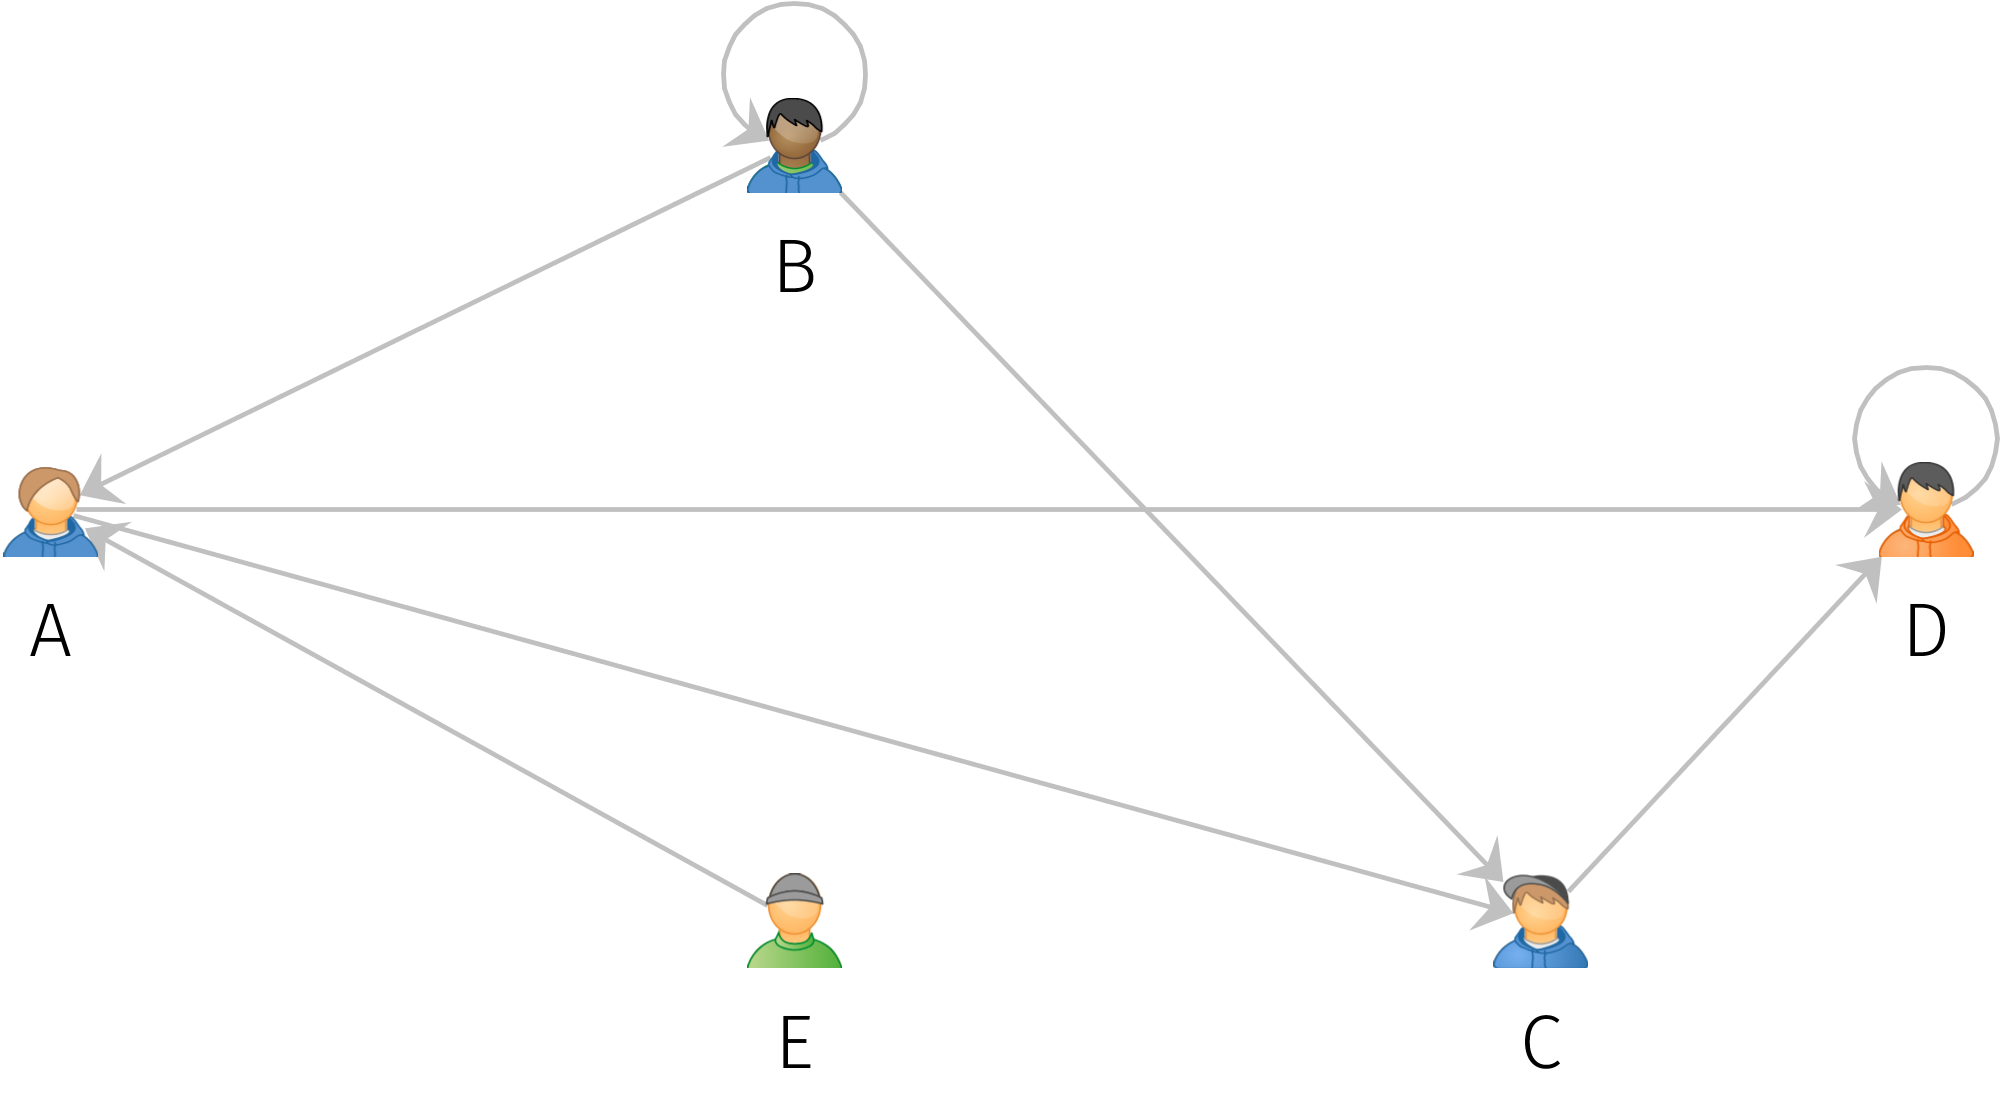
\includegraphics[width=7cm]{graphes/img/graphe1.png}
\end{center}
Ces résultats permettent de produire un \textit{graphe orienté} :
\begin{itemize}
    \item 	les \textit{sommets du graphe} représentent les personnes;
    \item 	les \textit{arêtes} sont des flèches qui représentent le fait que la personne de départ aime les messages de celle d'arrivée.
\end{itemize}
On peut aussi représenter les résultats dans un tableau :
\begin{center}
    \tabstyle[UGLiBlue]
    \begin{tabular}{c|c|c|c|c|c}
        \hline\cellcolor{white}
                                                          & \cellcolor{UGLiOrange}\ccell A & \cellcolor{UGLiOrange}\ccell B & \cellcolor{UGLiOrange}\ccell C & \cellcolor{UGLiOrange}\ccell D & \cellcolor{UGLiOrange}\ccell E \\
        \hline
        \cellcolor{UGLiOrange}\ccell aime les messages de & C,D                            & B,C                            & D                              & D                              & A                              \\
        \hline
    \end{tabular}
\end{center}

On peut aussi recopier le tableau en donnant pour chaque personne la liste de ses  «  followers »  (personnes qui ont aimé ses messages) :

\begin{center}
    \tabstyle[UGLiBlue]
    \begin{tabular}{c|c|c|c|c|c}
        \hline\cellcolor{white}
                                               & \cellcolor{UGLiOrange}\ccell A & \cellcolor{UGLiOrange}\ccell B & \cellcolor{UGLiOrange}\ccell C & \cellcolor{UGLiOrange}\ccell D & \cellcolor{UGLiOrange}\ccell E \\
        \hline
        \cellcolor{UGLiOrange}\ccell followers & B,E                            & B                              & A,B                            & A,C,D                          & ---                            \\
        \hline
    \end{tabular}
\end{center}
On peut aussi présenter les données ainsi :
\begin{center}
    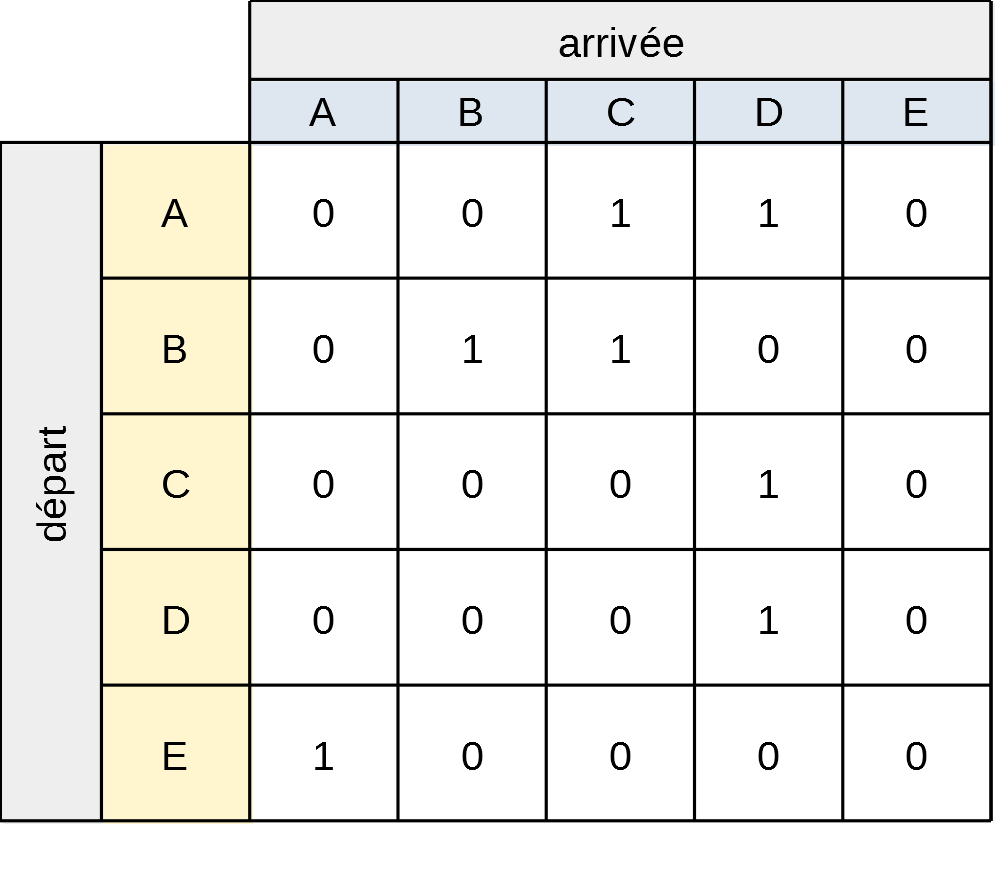
\includegraphics[width=7cm]{graphes/img/prematrice.png}
\end{center}
Il y a donc plusieurs manières de représenter un graphe orienté.

\subsection{Organiser un graphe orienté}

On considère des individus qui ont infectés par une maladie et on place une flèche pour signifier que tel individu a contaminé tel autre individu.\\
On obtient ce résultat :
\begin{center}
    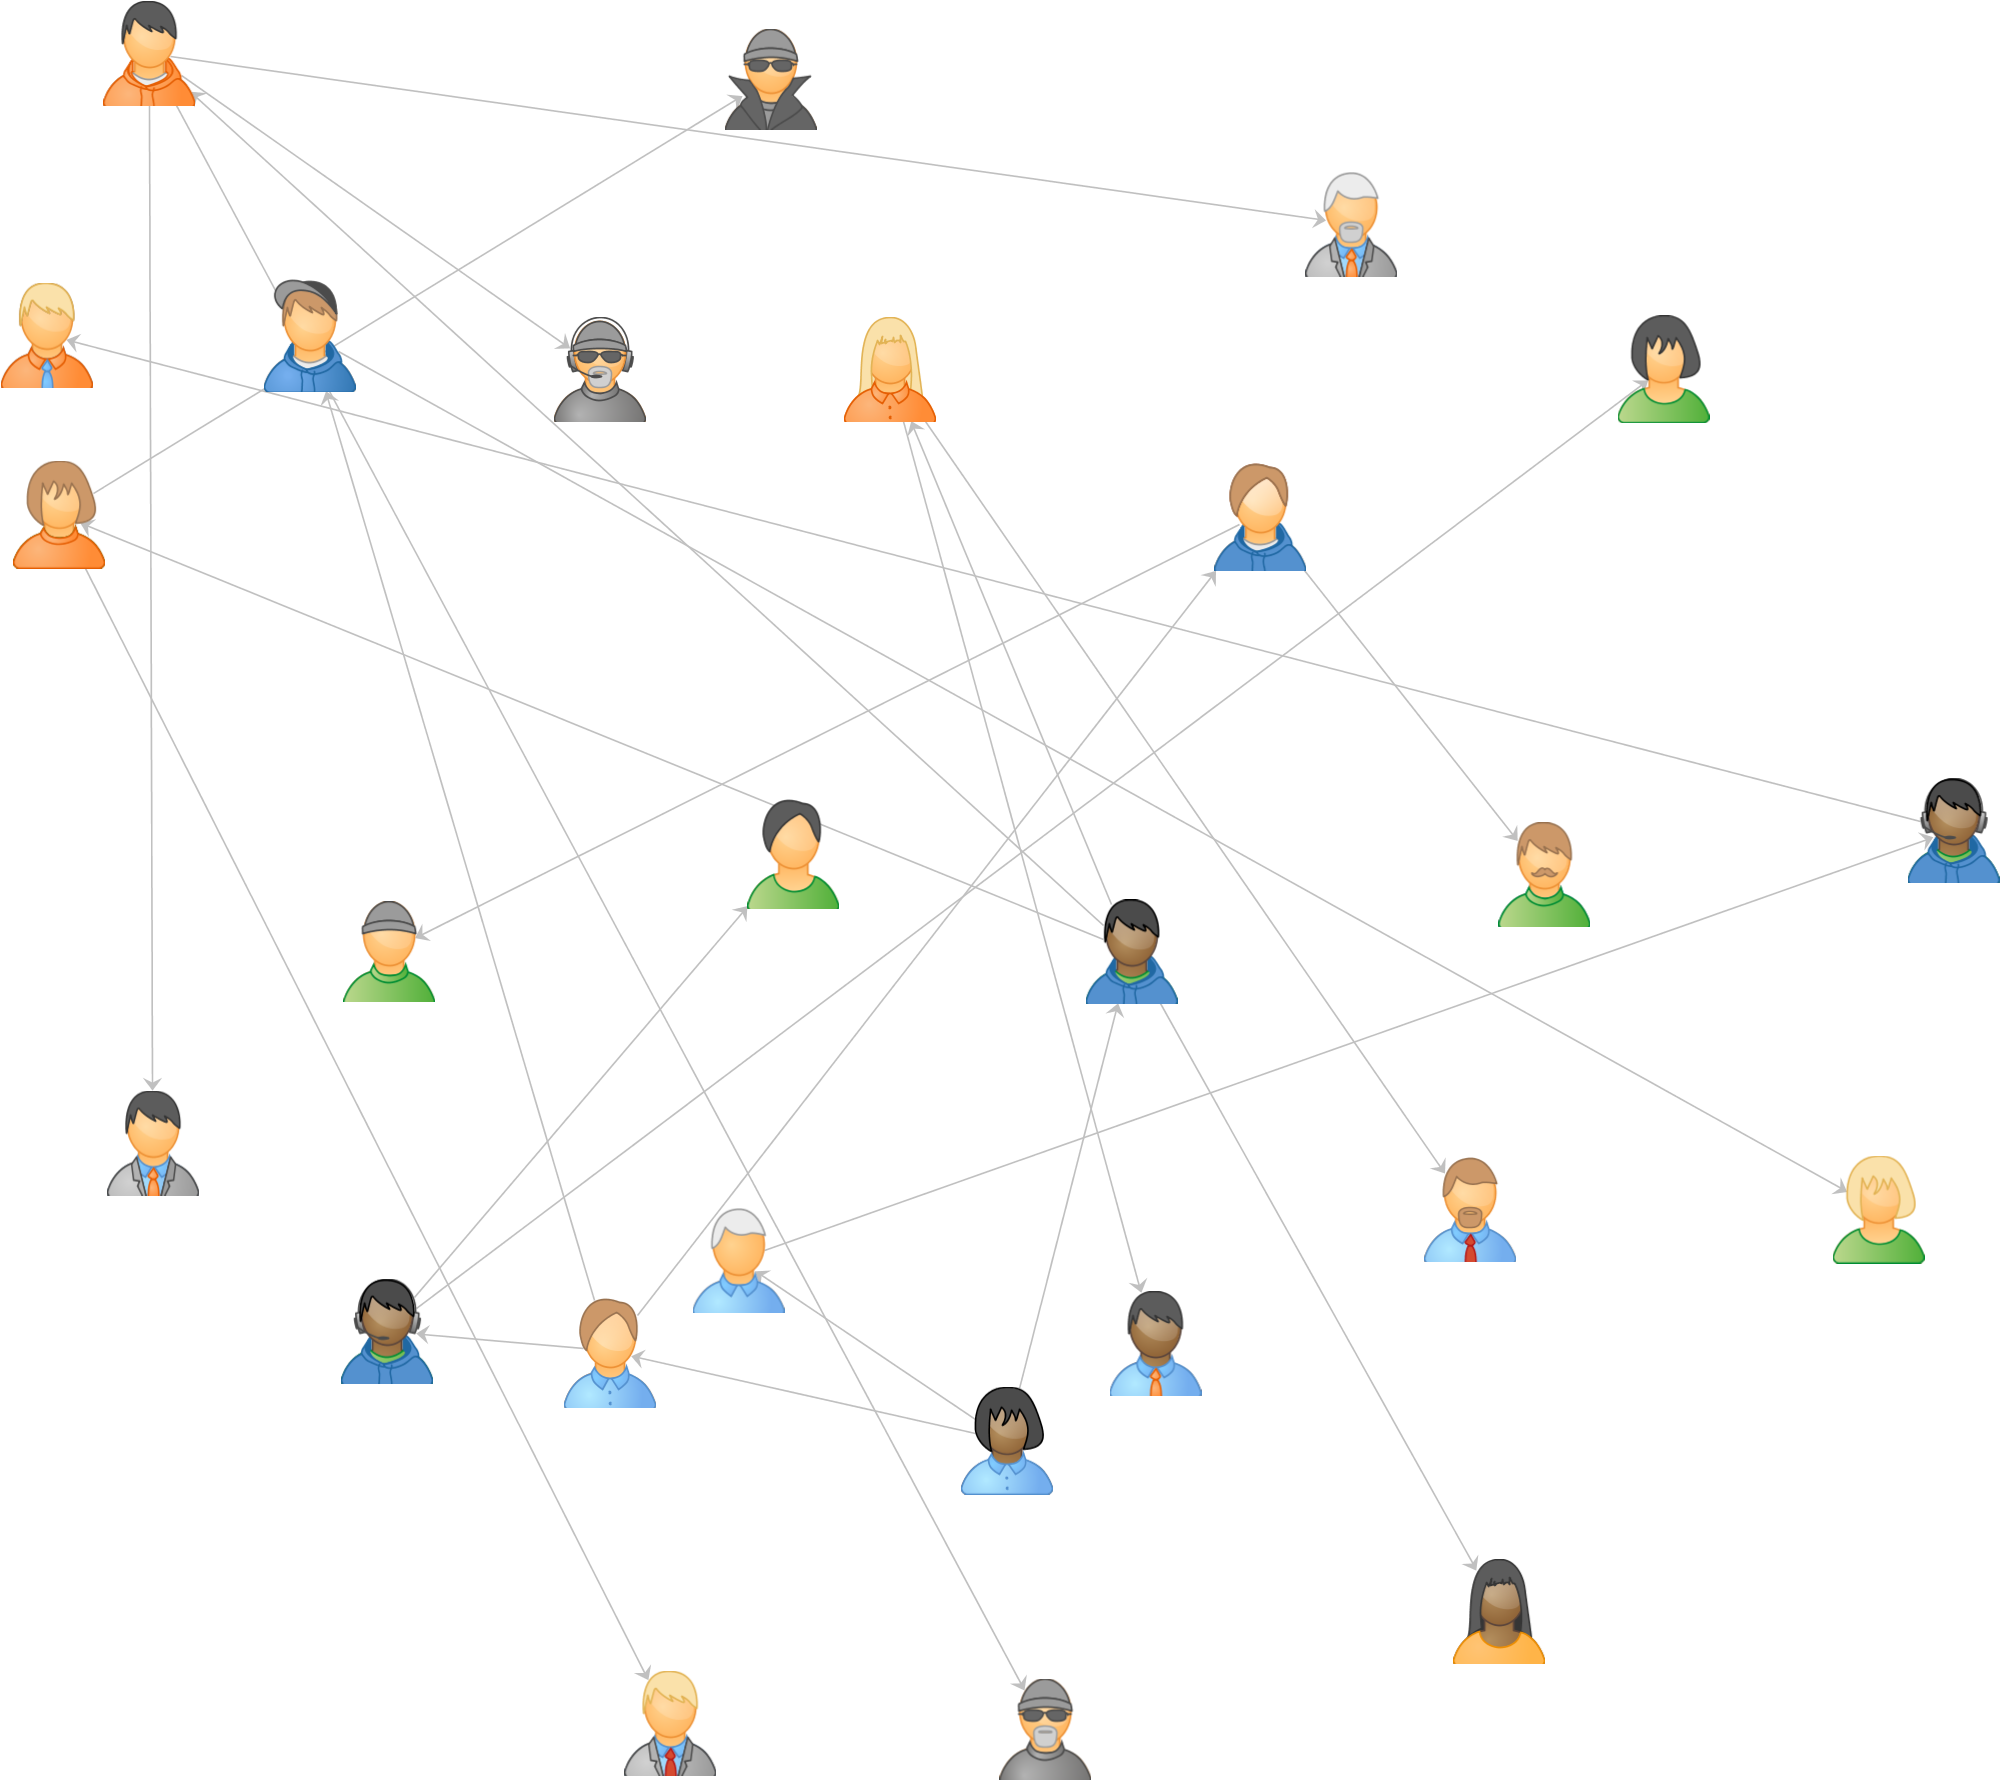
\includegraphics[width=7cm]{graphes/img/graphe2_random.png}
\end{center}
C'est le fouillis, n'est-ce pas ? \\
En déplaçant les sommets du graphe on peut le présenter ainsi :
\begin{center}
    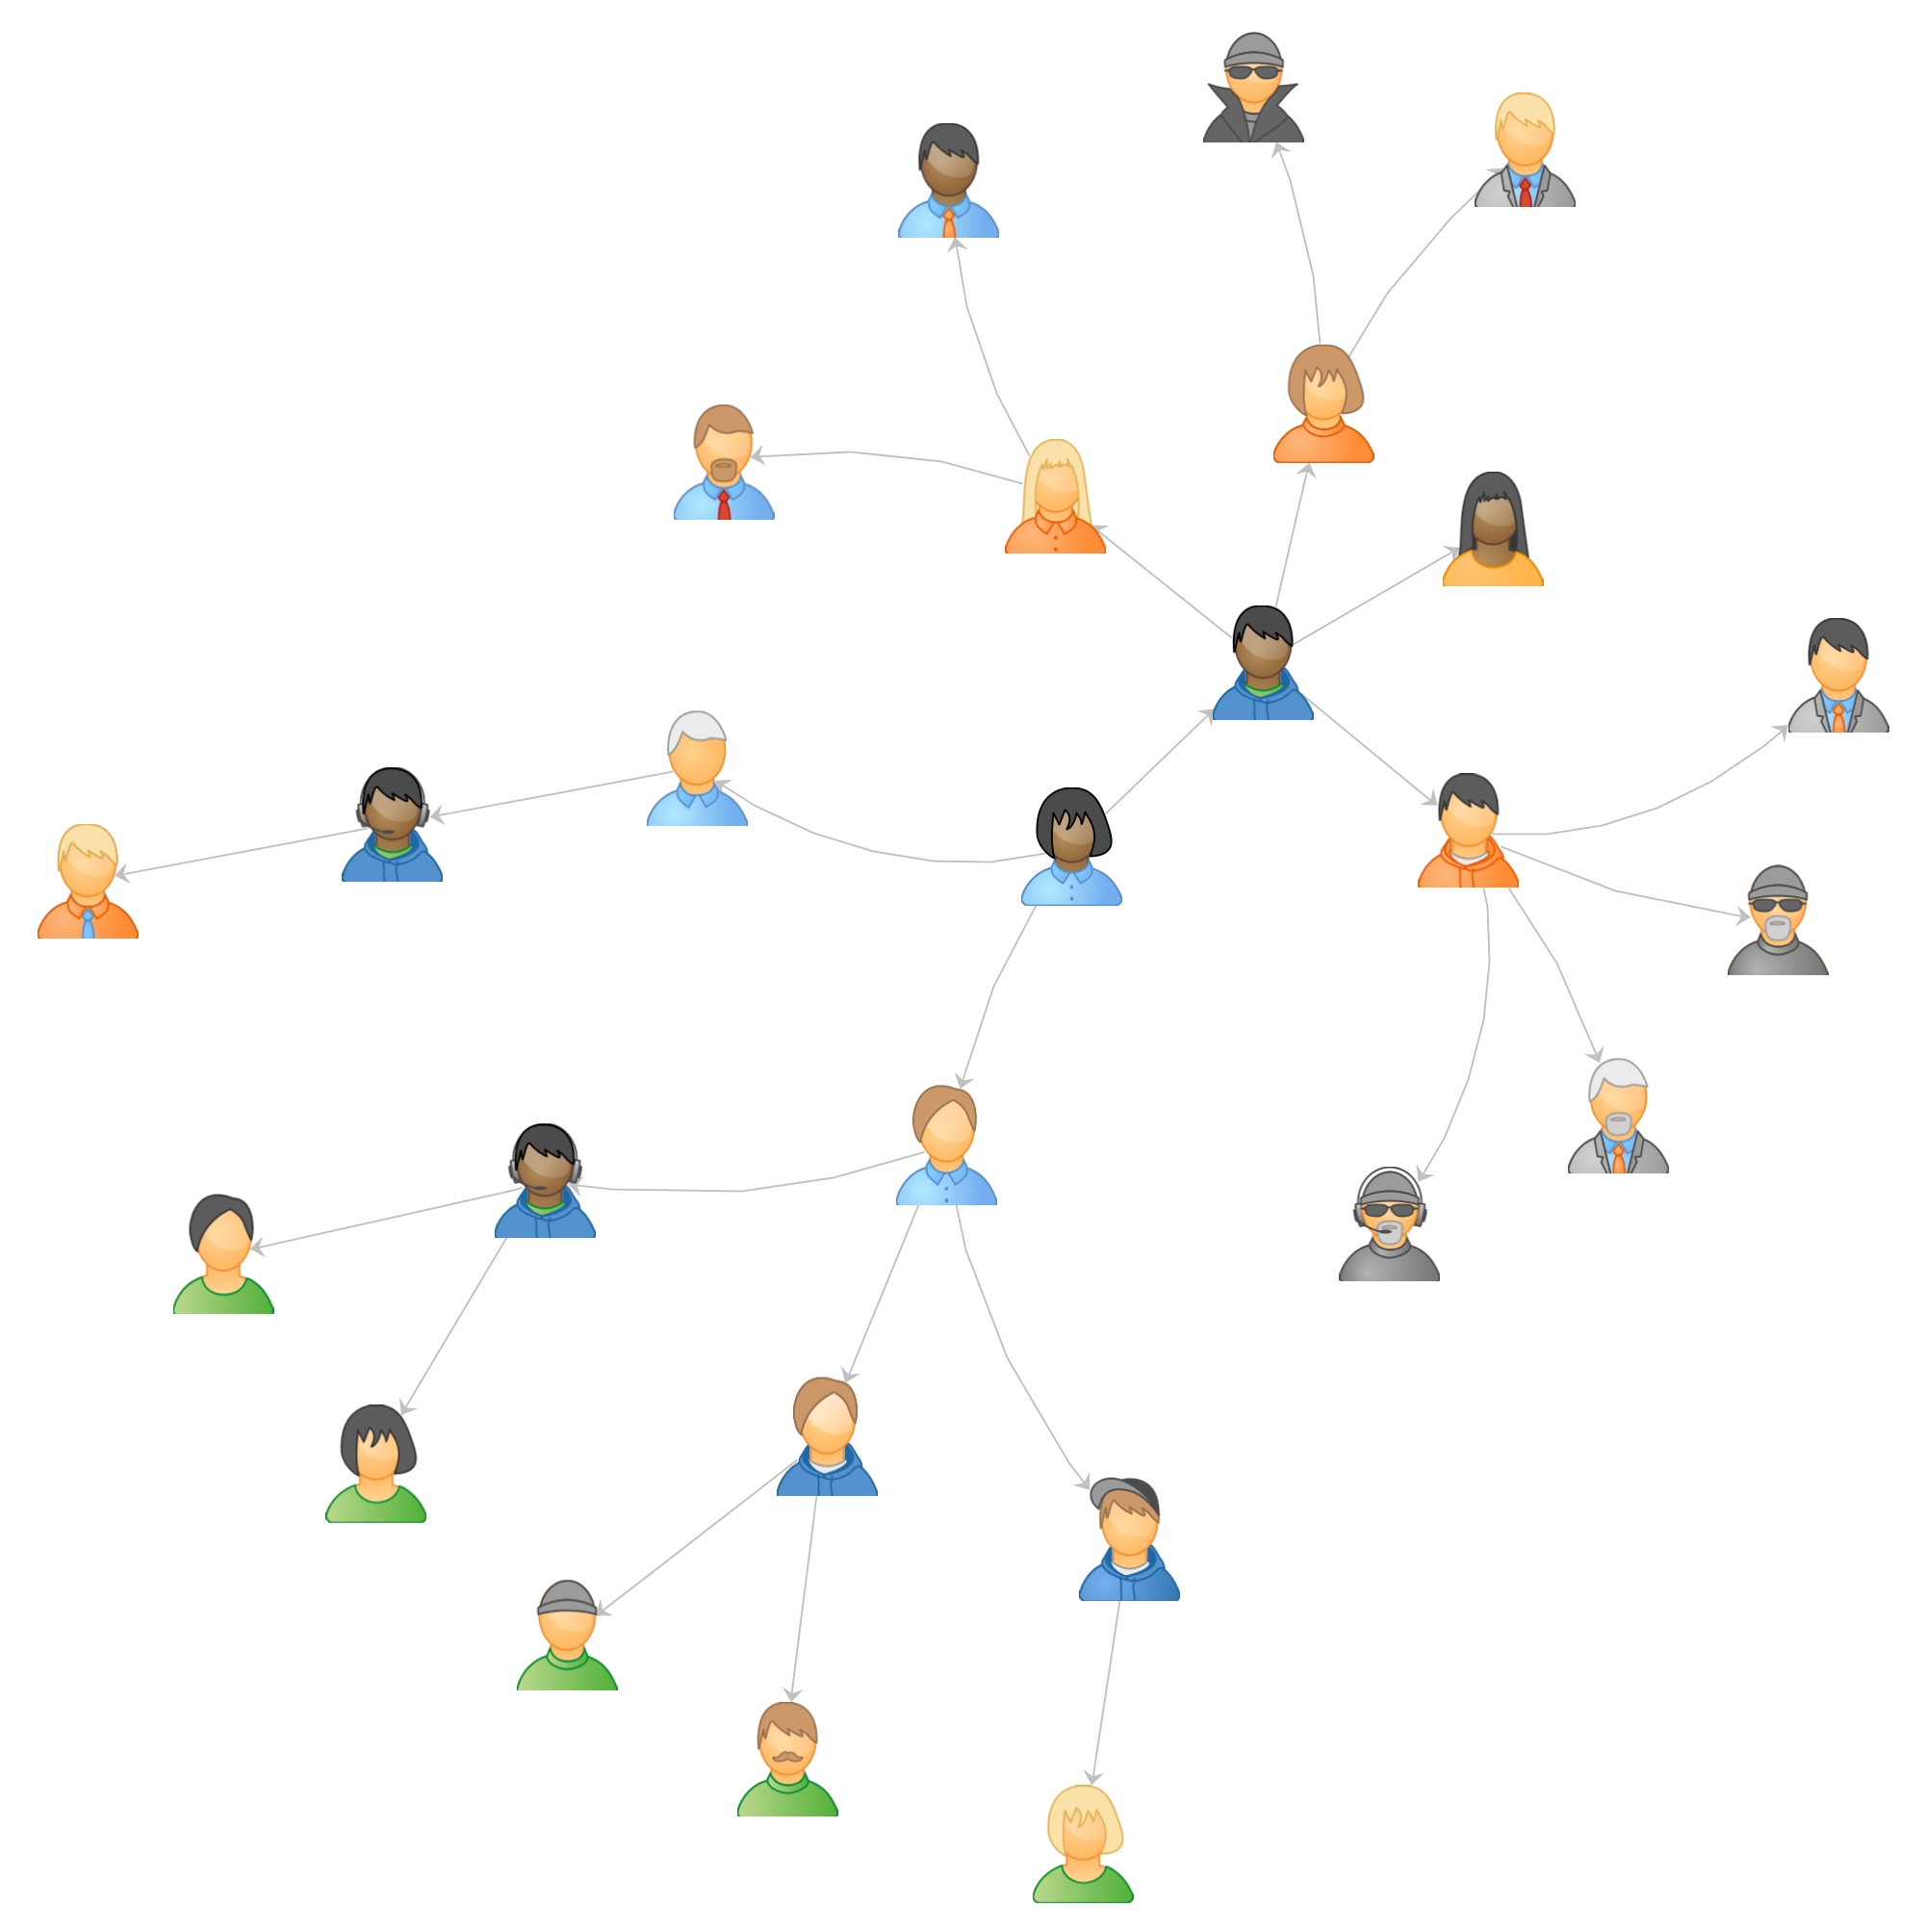
\includegraphics[width=7cm]{graphes/img/graphe2_radial.png}
\end{center}
C'est le même graphe mais on y voit plus clair... et on y voit encore plus clair comme ça :
\begin{center}
    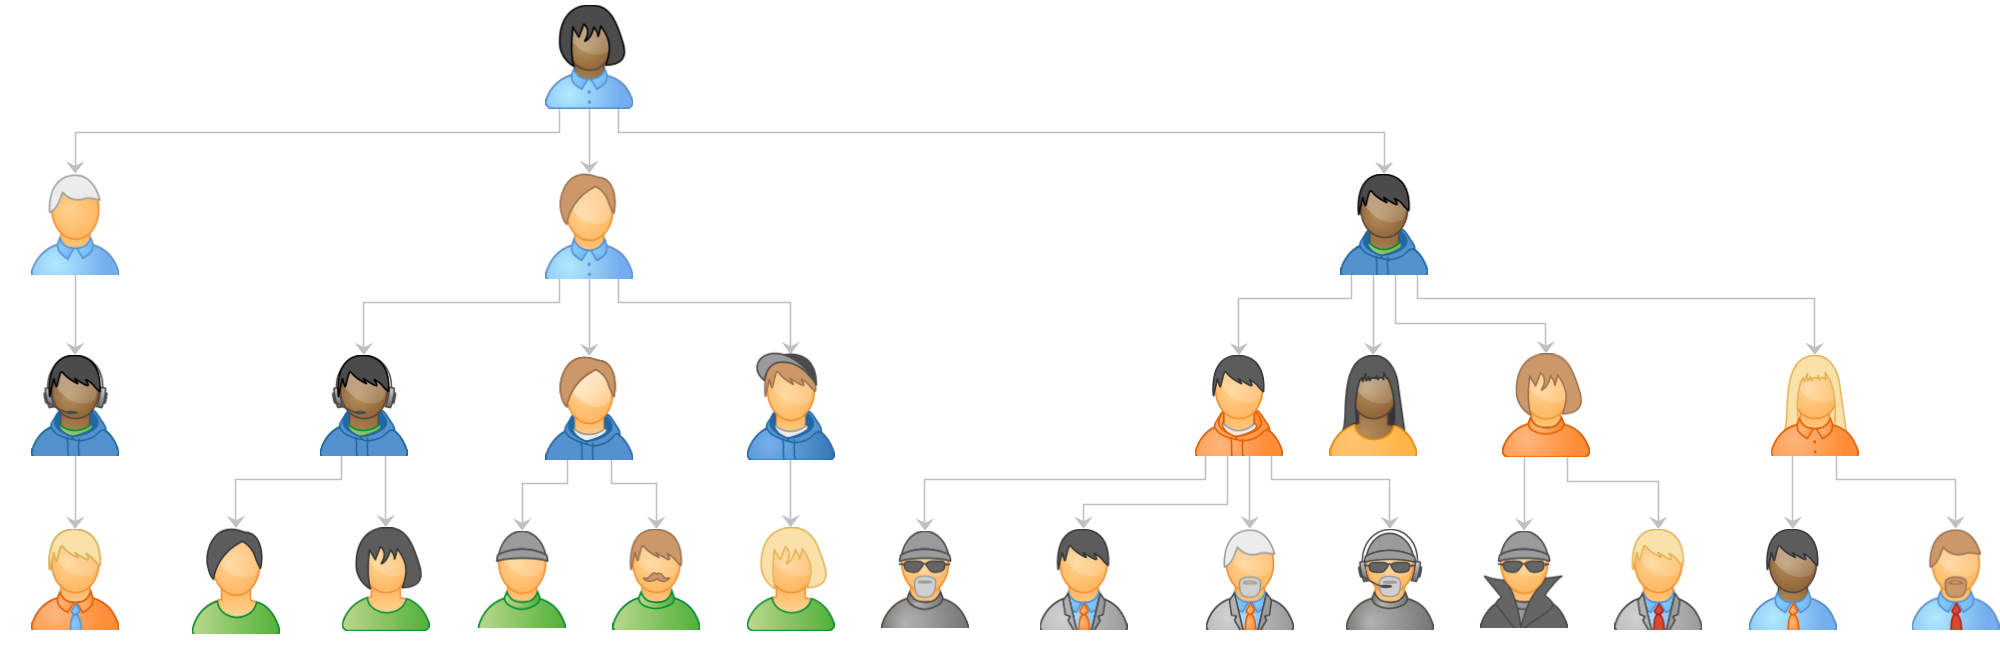
\includegraphics[width=7cm]{graphes/img/graphe2_tree.png}
\end{center}
On voit clairement le  «  patient zéro » . On peut aussi rajouter des flèches quand la contamination n'est pas directe mais s'est faite  «  par une ou plusieurs personnes interposées » . On obtient ceci
\begin{center}
    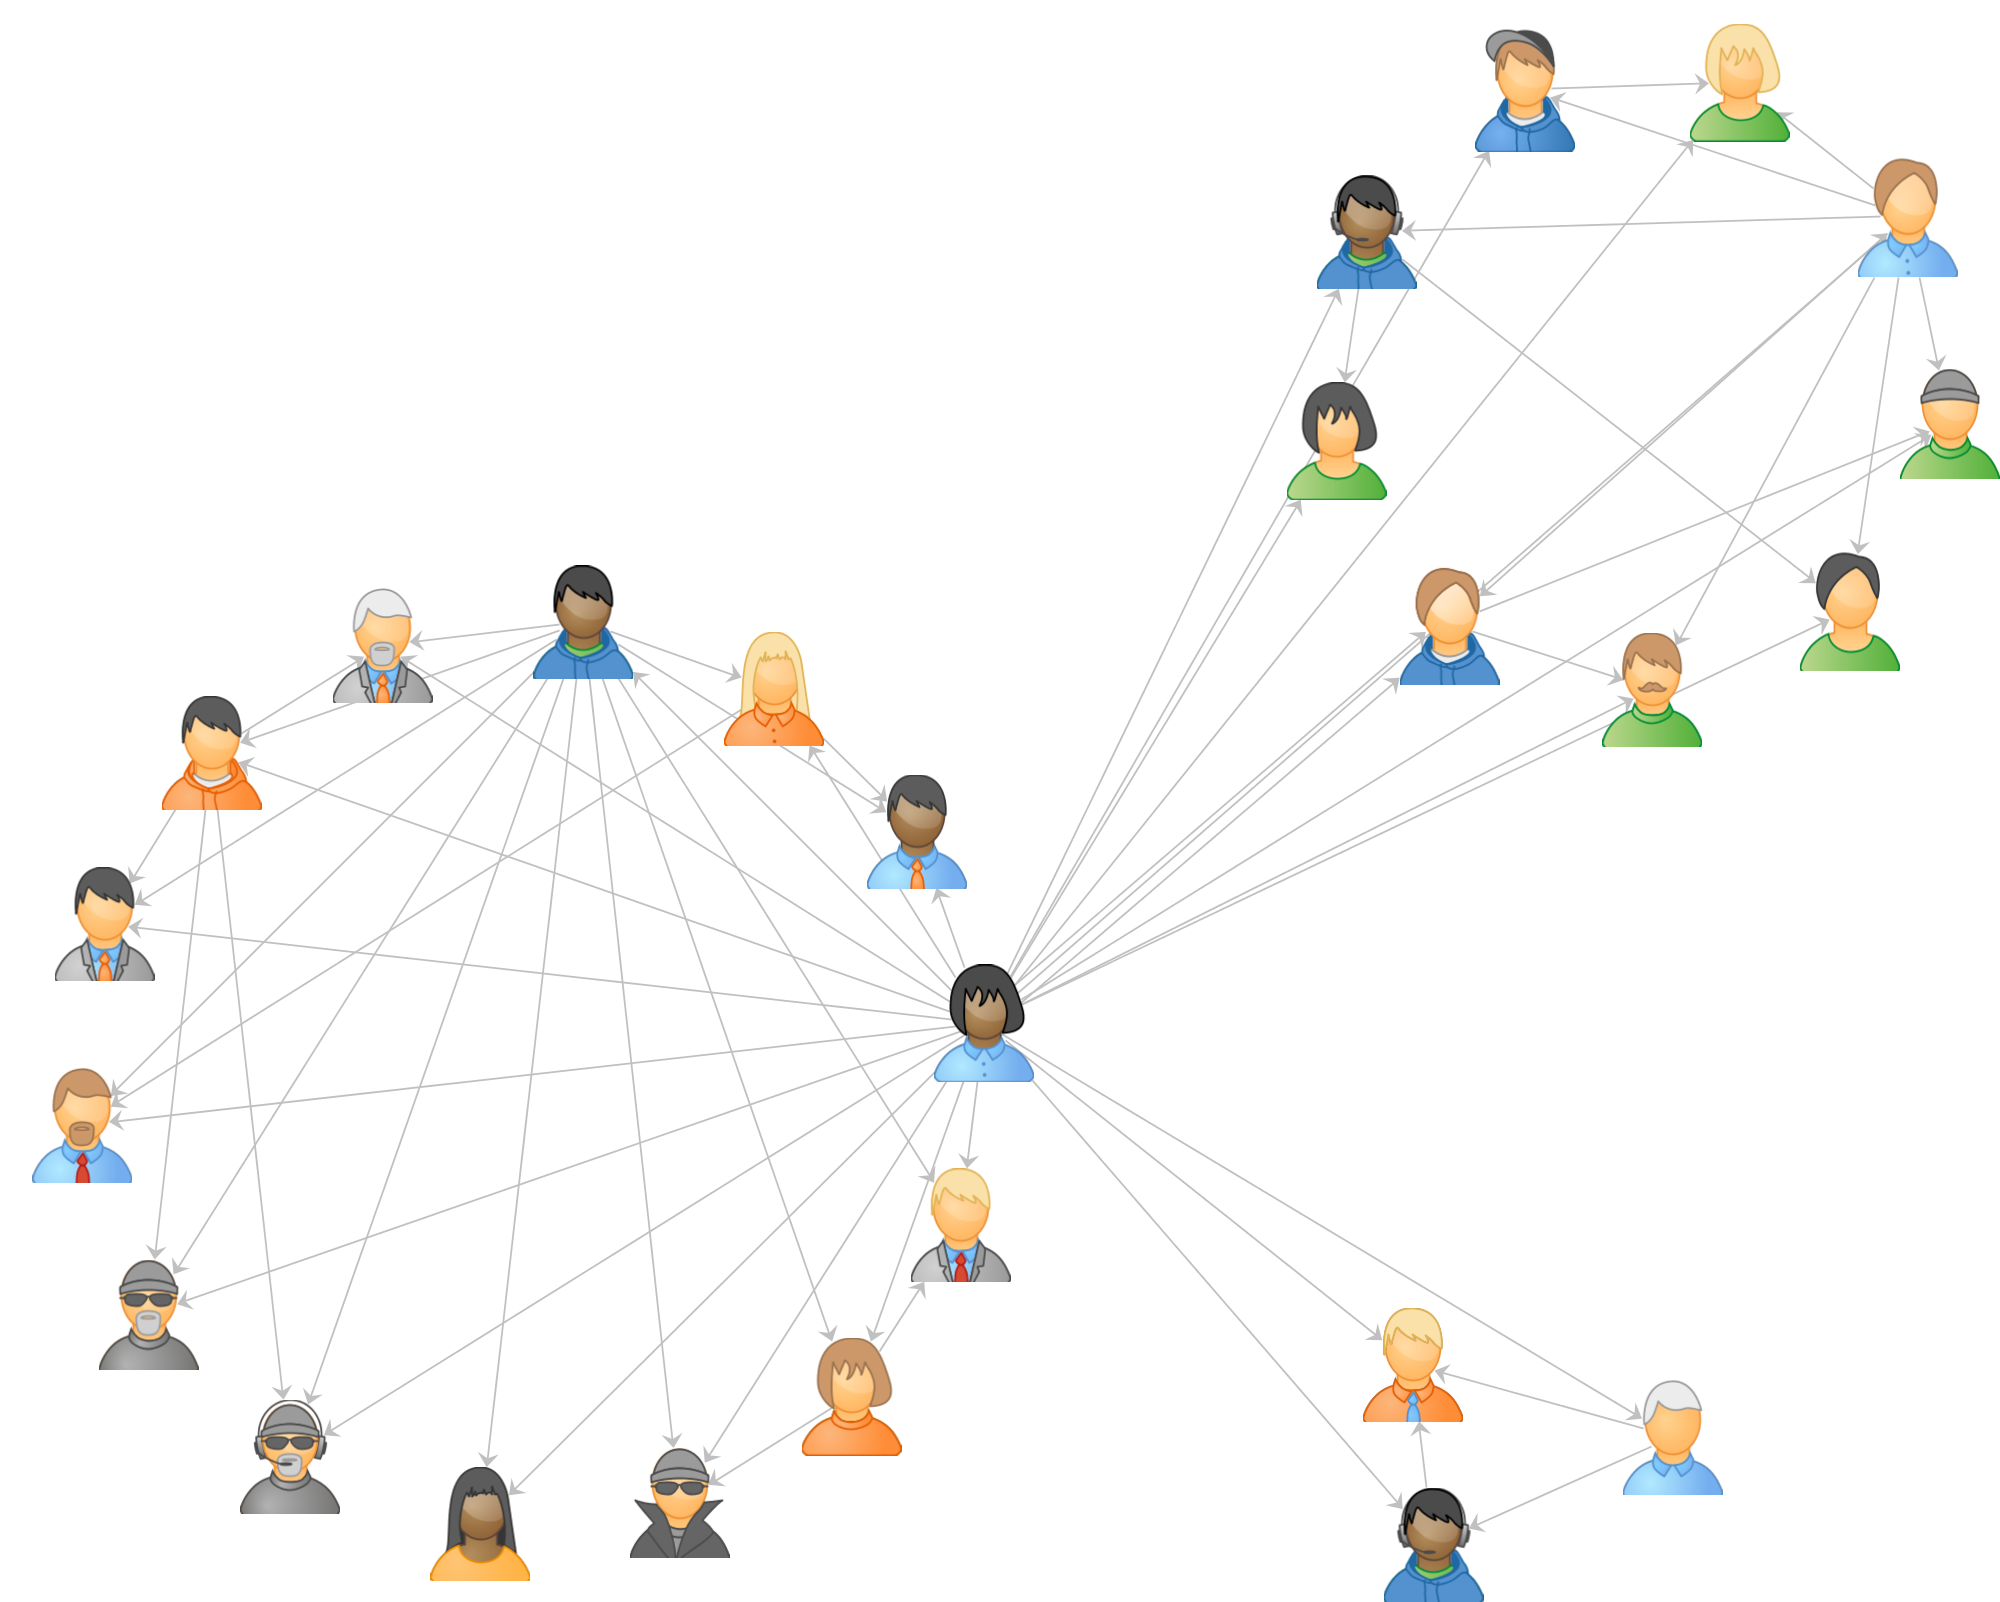
\includegraphics[width=7cm]{graphes/img/graphe2_transitif.png}
\end{center}
Le but de ce chapitre est de formaliser tout cela (et plus).

\section{Représentations d'un graphe orienté}
\subsection{Premières notions}
\begin{definition}[ : graphe, sommet, arc]
    Un graphe orienté, c'est la donnée de
    \begin{itemize}
        \item 	un ensemble $S=\lbrace s_1;\,...;\,s_n\rbrace$ de \textit{sommets};
        \item 	un ensemble $A$ composé d'\textit{arcs} du type $(s_i;\,s_j)$, qui indiquent qu'il y a  «  une flèche »  partant du sommet $s_i$ et allant au sommet $s_j$.:\\ $s_i$ est appelé l'\textit{origine} de l'arc et $s_j$ son \textit{extrémité}.
    \end{itemize}
\end{definition}

\begin{exemple}[]
    Ici l'ensemble des sommets est $\lbrace A;\,B;\,C;\,D\rbrace$.\\
    L'ensemble des arcs est :\\
    $\lbrace (A;B);\,(B;A);\,(B;C);\,(B;D);\,(C;D)\rbrace$.
    \begin{center}
        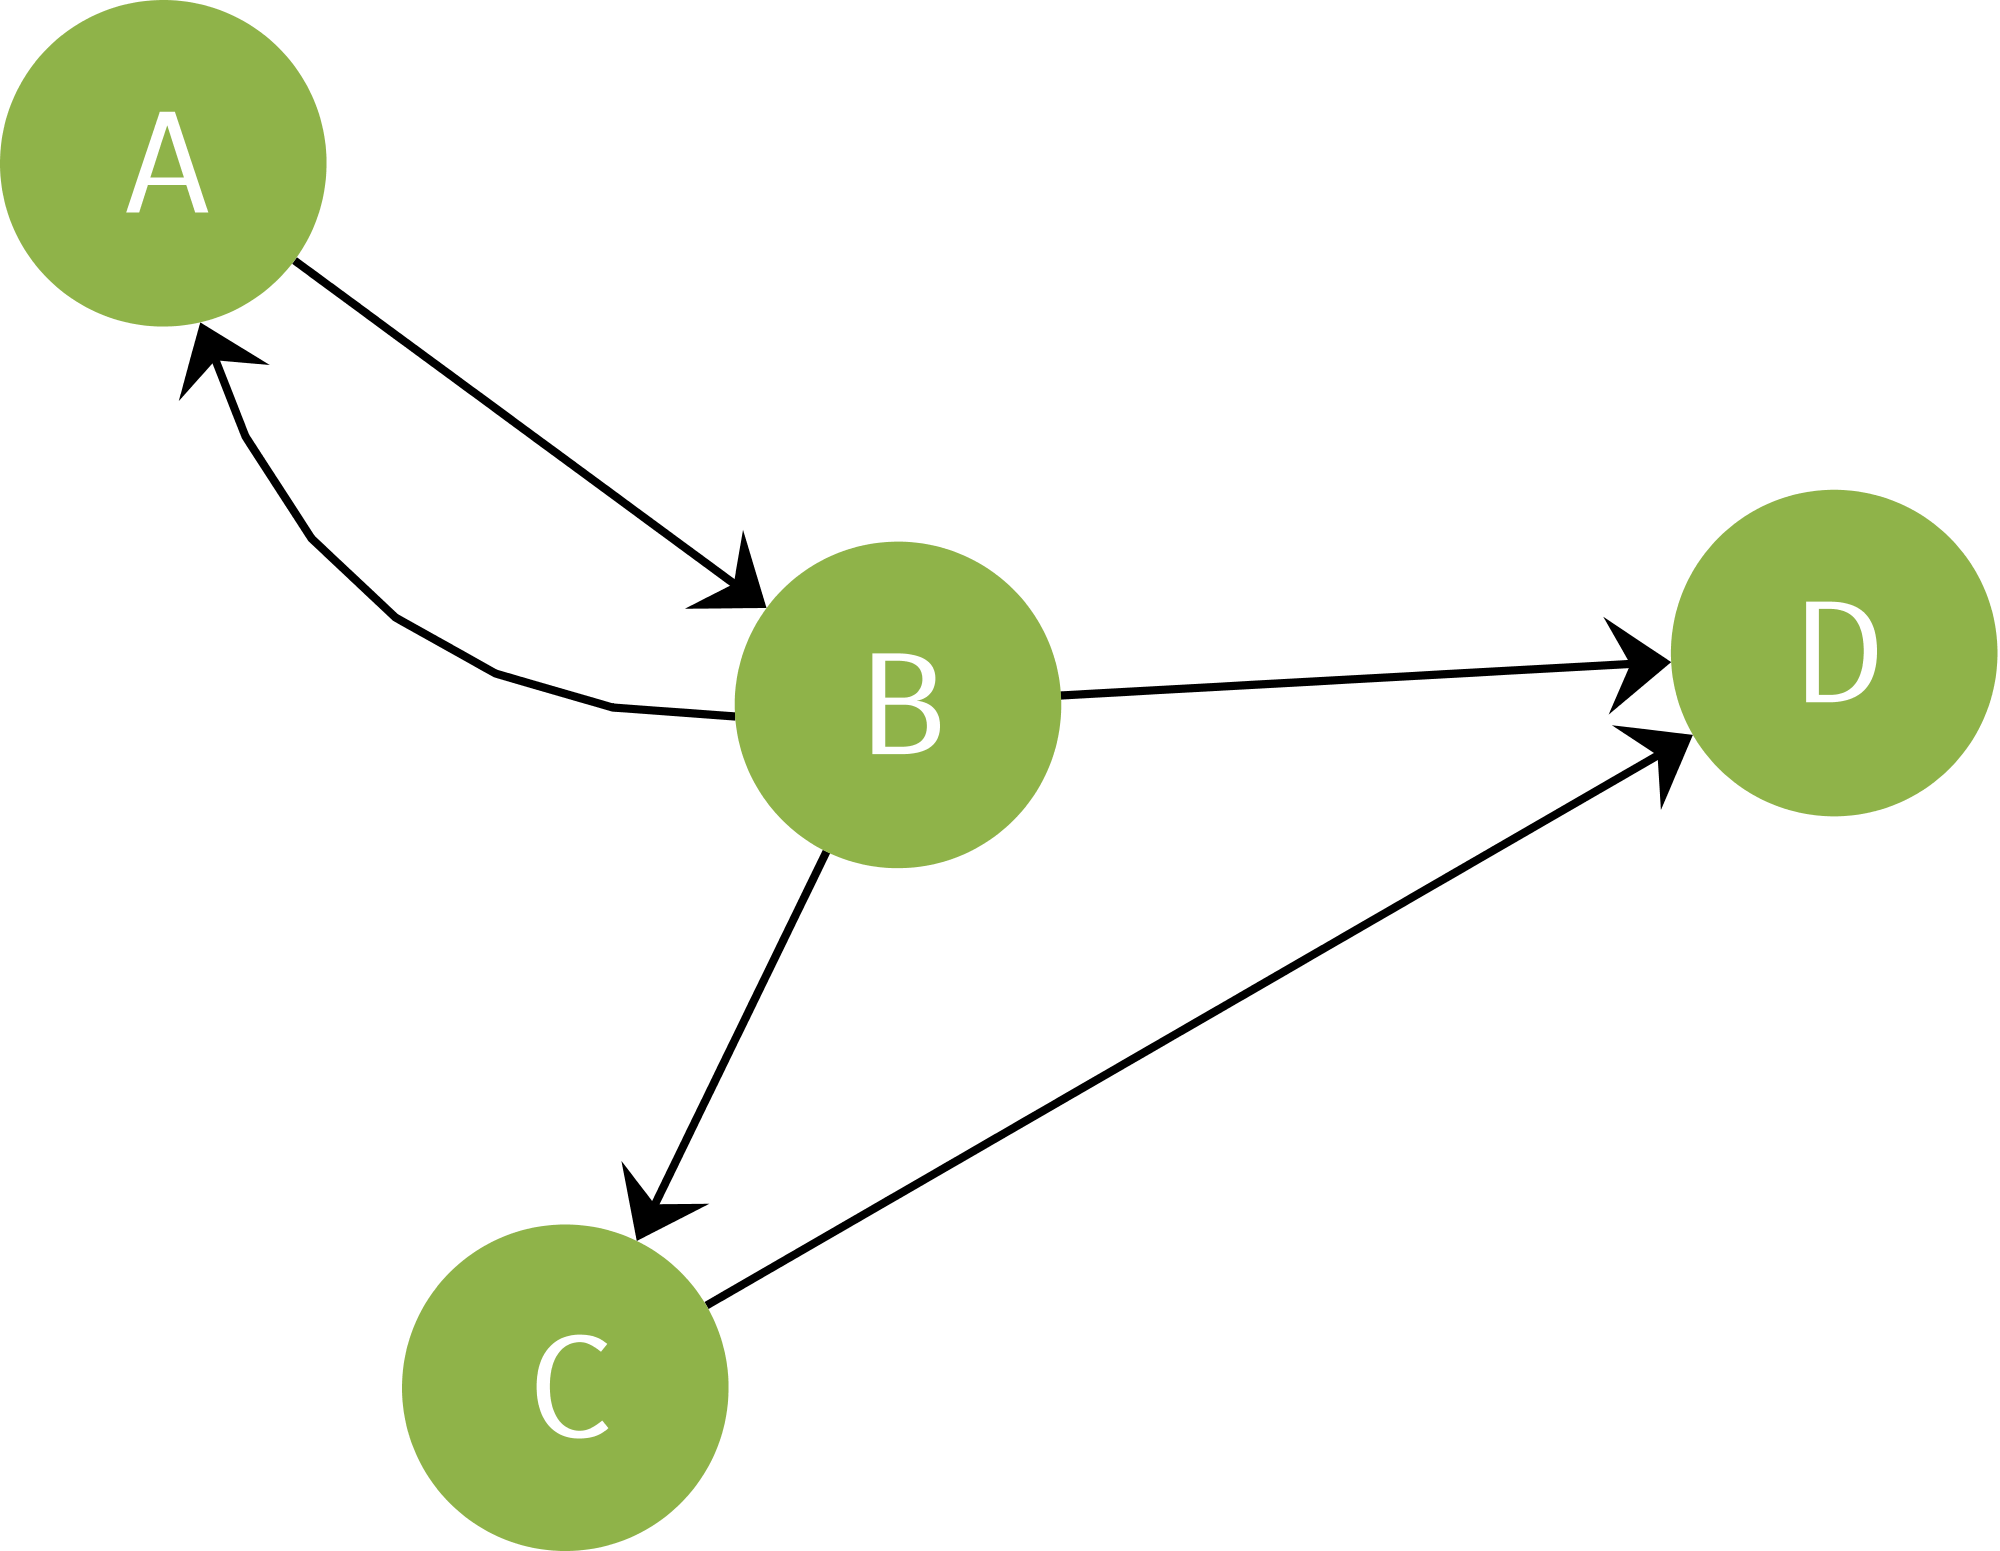
\includegraphics[width=5cm]{graphes/img/ex_graphe_oriente.png}
    \end{center}
\end{exemple}

\begin{exercice}[]
    Donner l'ensemble des sommets et l'ensemble des arêtes du graphe suivant.
    \begin{center}
        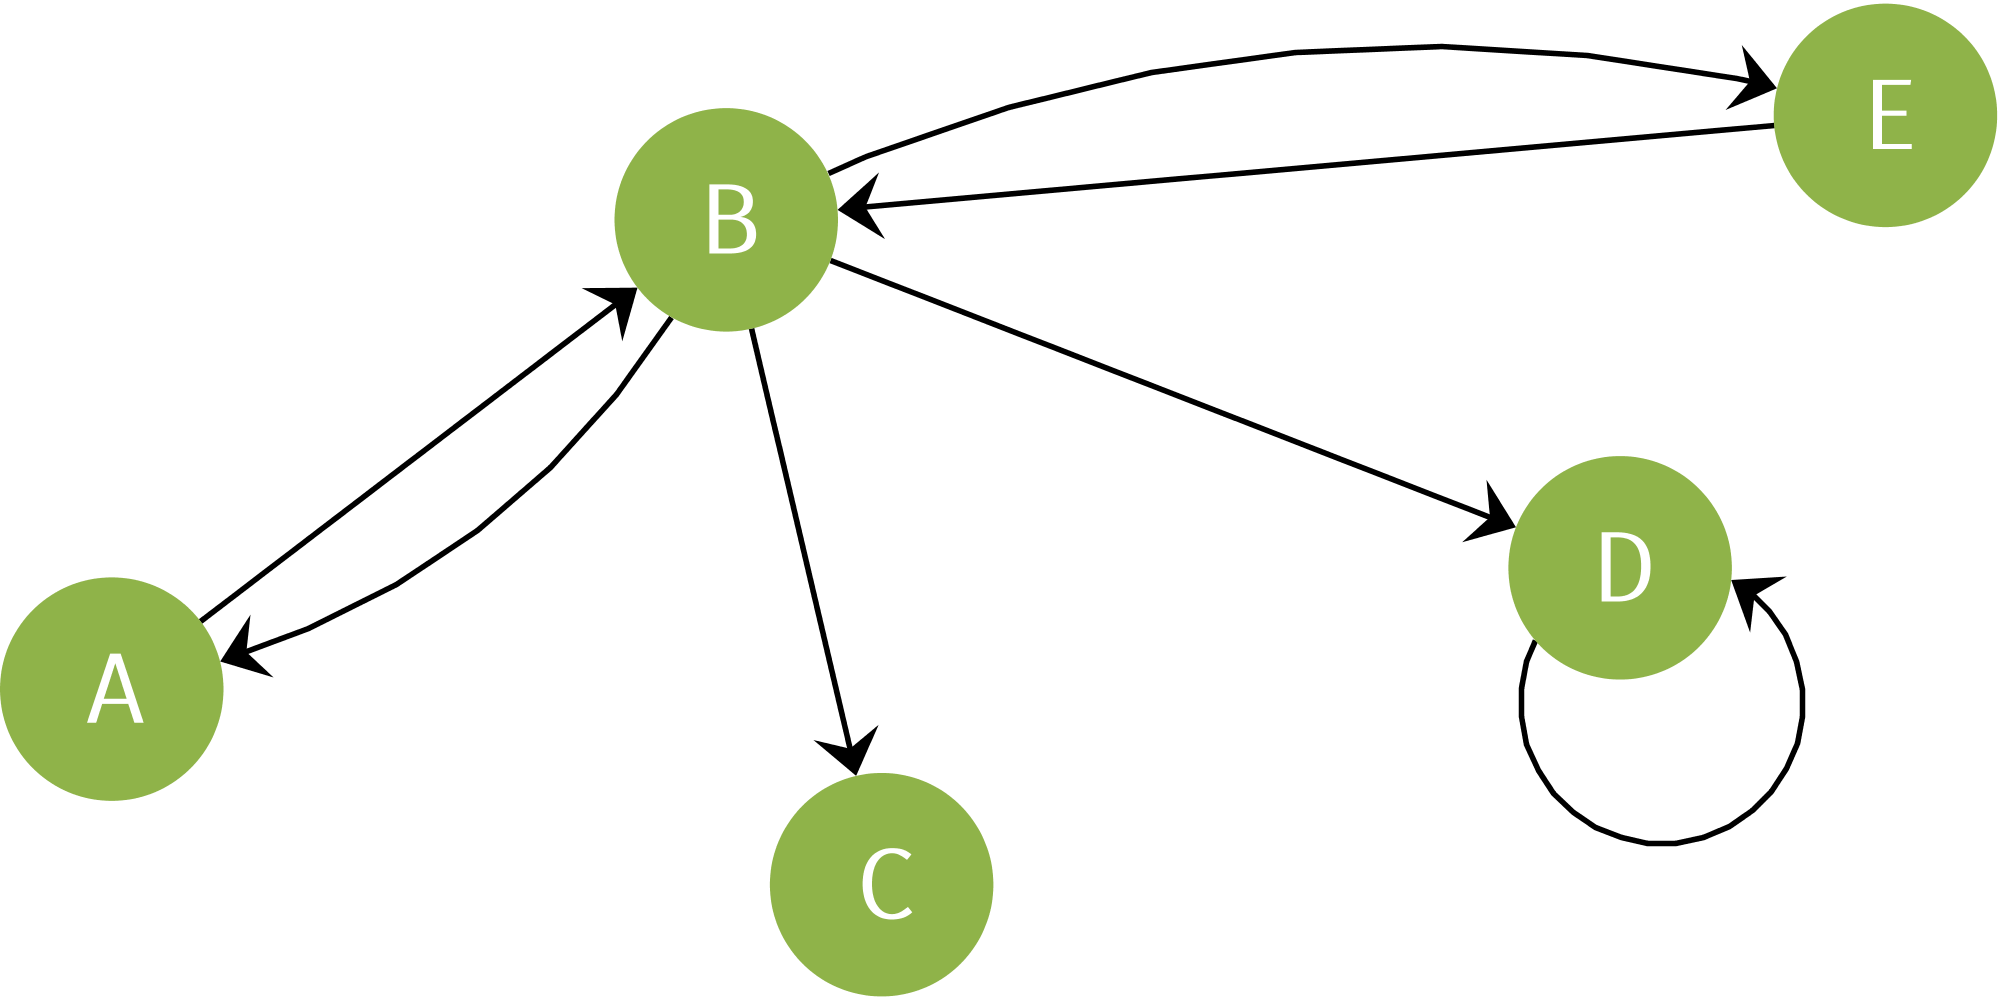
\includegraphics[width=7cm]{graphes/img/exo_graphe.png}
    \end{center}
\end{exercice}

\begin{definition}[ : boucle]
    Un arc dont l'origine et l'extrémité sont confondues d'appelle une \textit{boucle}.
\end{definition}

\subsection{Successeurs, prédécesseurs}

\begin{definition}[ : successeur, prédécesseur]
    Soit un graphe de sommets $S$ et d'arcs $A$. Soit $s$ un sommet.\\
    On note $\Gamma^+(s)$ l'ensemble des \textit{successeurs de $s$}.\\
    C'est l'ensemble des extrémités des arcs \textit{partant de} $s$.\\
    De même, on note $\Gamma^-(s)$ l'ensemble des \textit{prédécesseurs de $s$}.\\
    C'est l'ensemble des origines des arcs \textit{arrivant sur} $s$.\\
\end{definition}

\begin{exemple}[s]
    Dans ce graphe, il y a 4 arcs d'origine D. Leurs extrémités sont les points C,D,E et F.\\ Ainsi $\Gamma^+(D)=\lbrace C;\,D;\,E;\,F\rbrace$.
    \begin{center}
        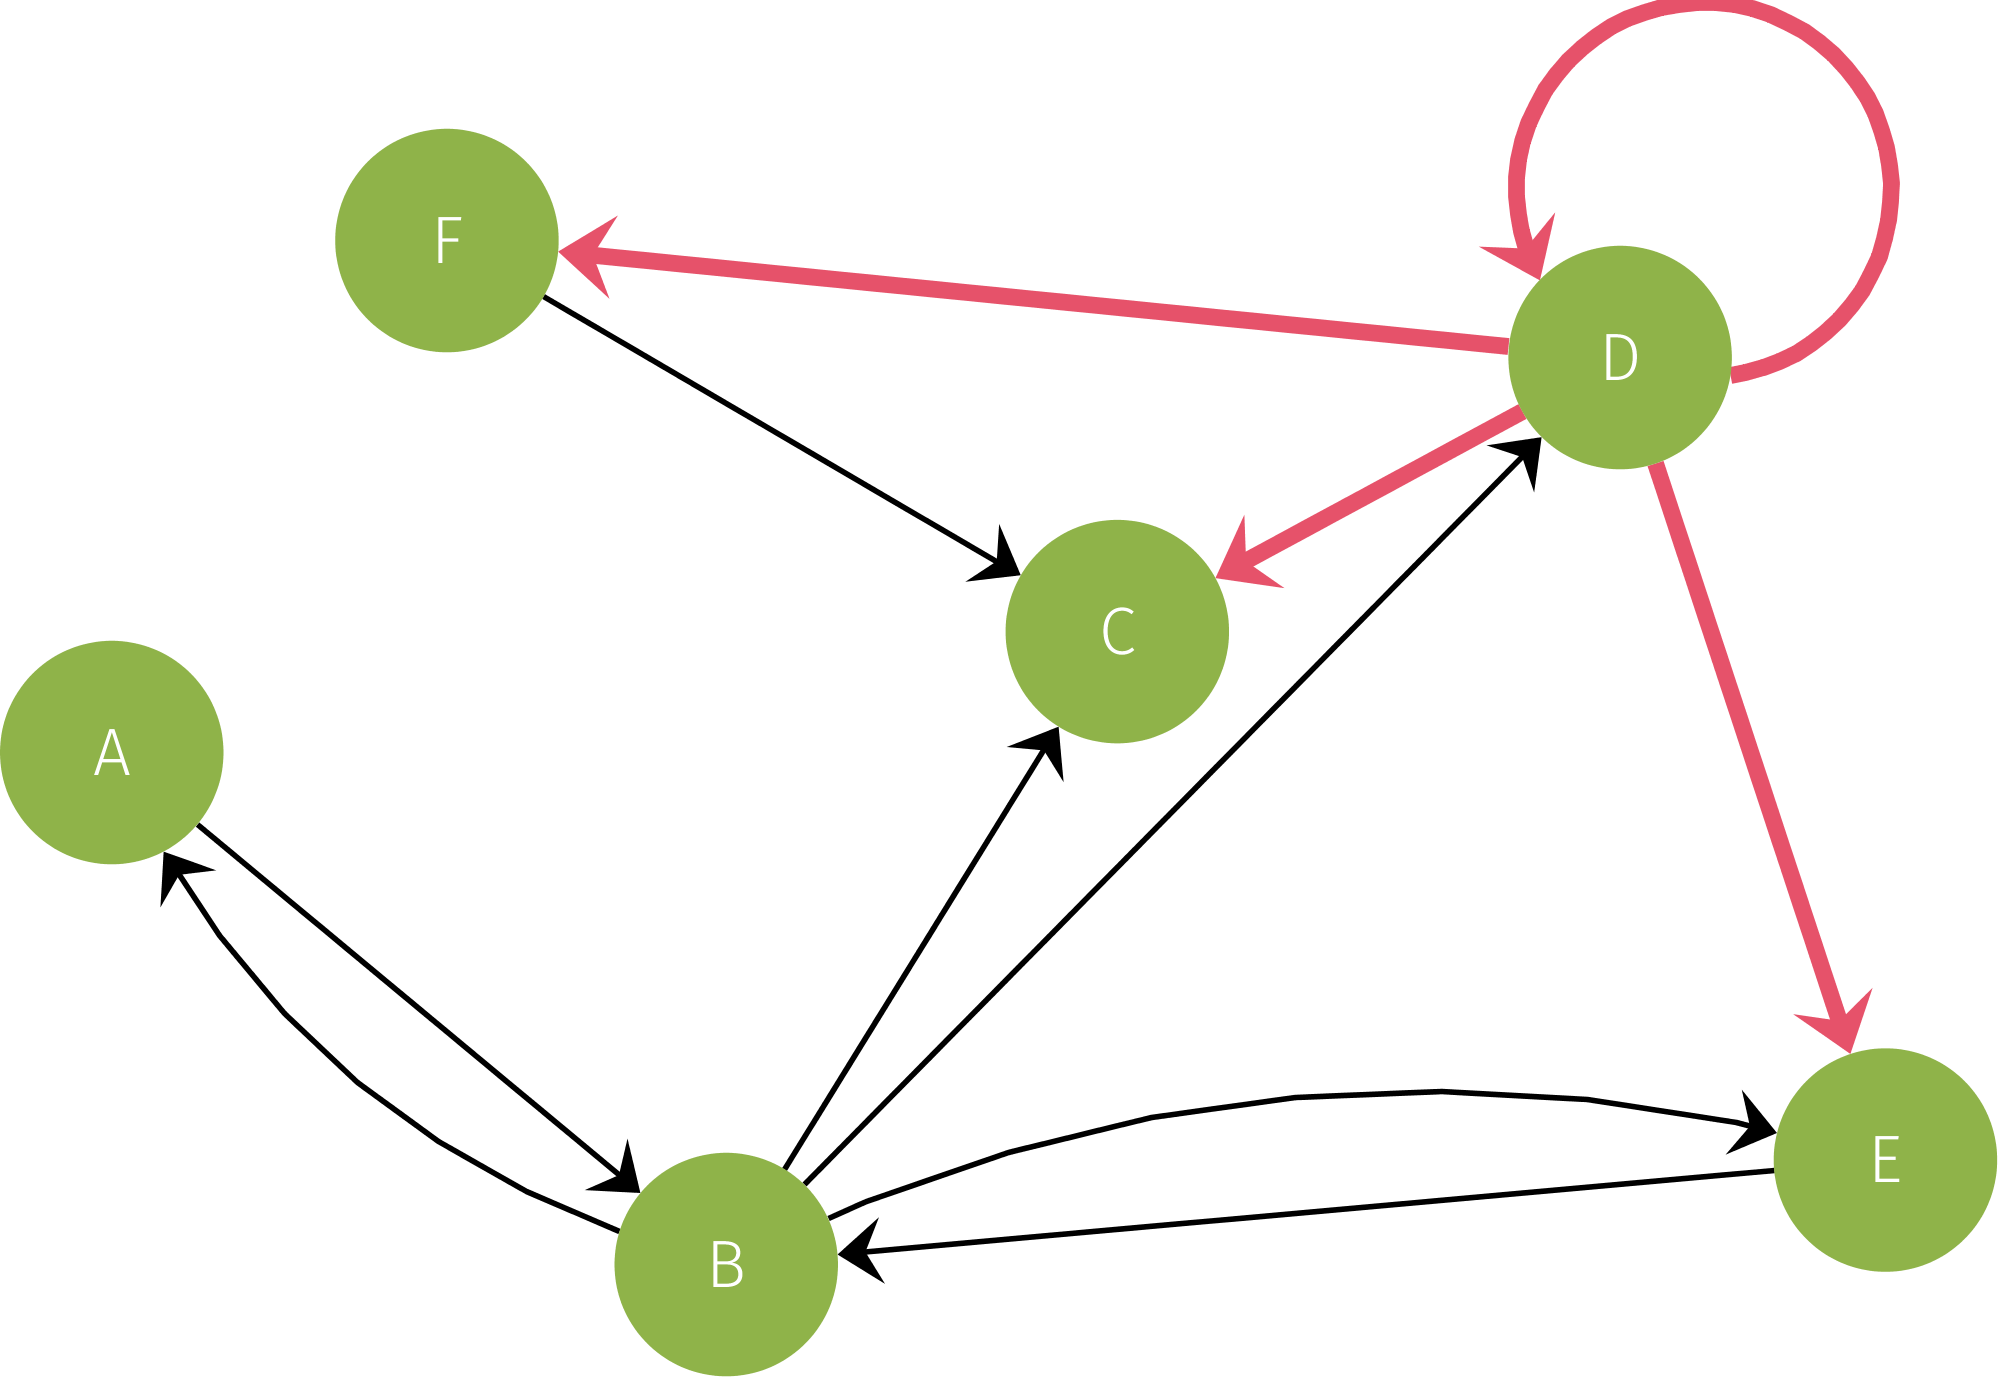
\includegraphics[width=7cm]{graphes/img/successeurs.png}
    \end{center}
    On peut retrouver le graphe à partir du tableau des successeurs.
    \begin{center}
        \tabstyle[UGLiBlue]
        \begin{tabular}{|c|c|c|c|c|c|c|}
            \hline
            \cellcolor{UGLiBlue}\ccell sommet      & \cellcolor{UGLiBlue}\ccell A & \cellcolor{UGLiBlue}\ccell B & \cellcolor{UGLiBlue}\ccell C & \cellcolor{UGLiBlue}\ccell D & \cellcolor{UGLiBlue}\ccell E & \cellcolor{UGLiBlue}\ccell F \\
            \hline
            \cellcolor{UGLiBlue}\ccell successeurs & B                            & A, C, E                      & ---                          & C, D, E, F                   & B                            & C                            \\
            \hline
        \end{tabular}
        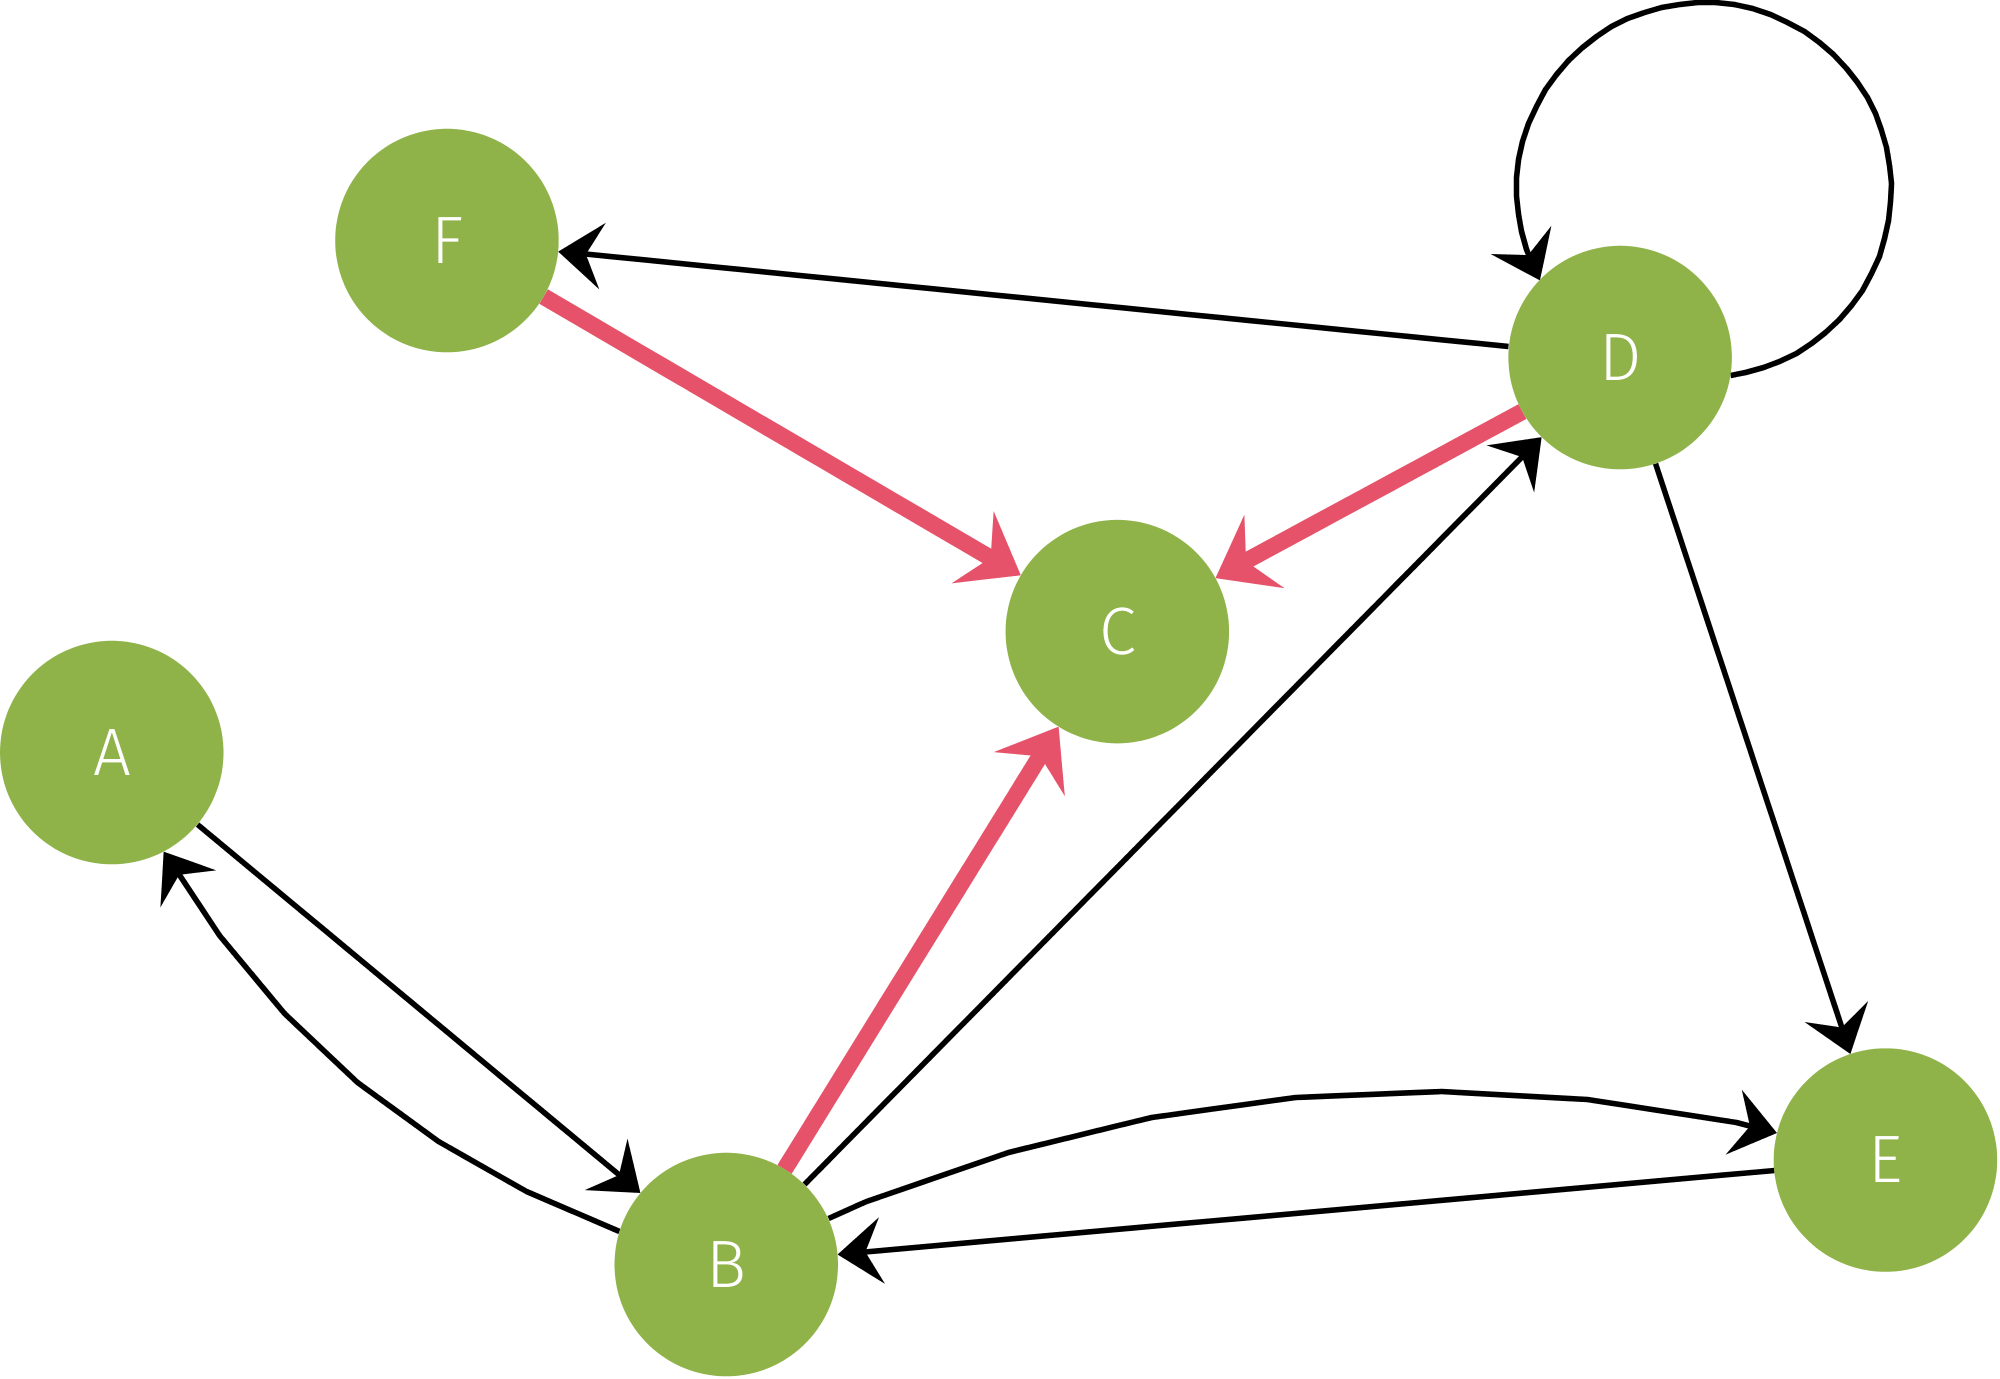
\includegraphics[width=7cm]{graphes/img/predecesseurs.png}
    \end{center}
    Dans ce graphe, il y a 3 arcs d'extrémité C.\\
    Leurs origines sont les points B,D et F.\\ Ainsi $\Gamma^-(C)=\lbrace B;\,D;\,F\rbrace$.
    On peut retrouver le graphe à partir du tableau des prédécesseurs.
    \begin{center}
        \tabstyle[UGLiBlue]
        \begin{tabular}{|c|c|c|c|c|c|c|}
            \hline
            \rowcolor{UGLiBlue}\ccell sommet         & \ccell A & \ccell B & \ccell C & \ccell D & \ccell E & \ccell F \\
            \hline
            \cellcolor{UGLiBlue}\ccell prédécesseurs & B        & A, E     & B, D, F  & B, D     & B, D     & D        \\
            \hline
        \end{tabular}
    \end{center}
\end{exemple}

\begin{exercice}[]
    Pour chacun des graphes, donne le tableau des successeurs et celui des prédécesseurs (attention : pour le graphe de gauche, on a dessiné des arcs bidirectionnels, chacun compte pour 2 arcs).
    \begin{center}
        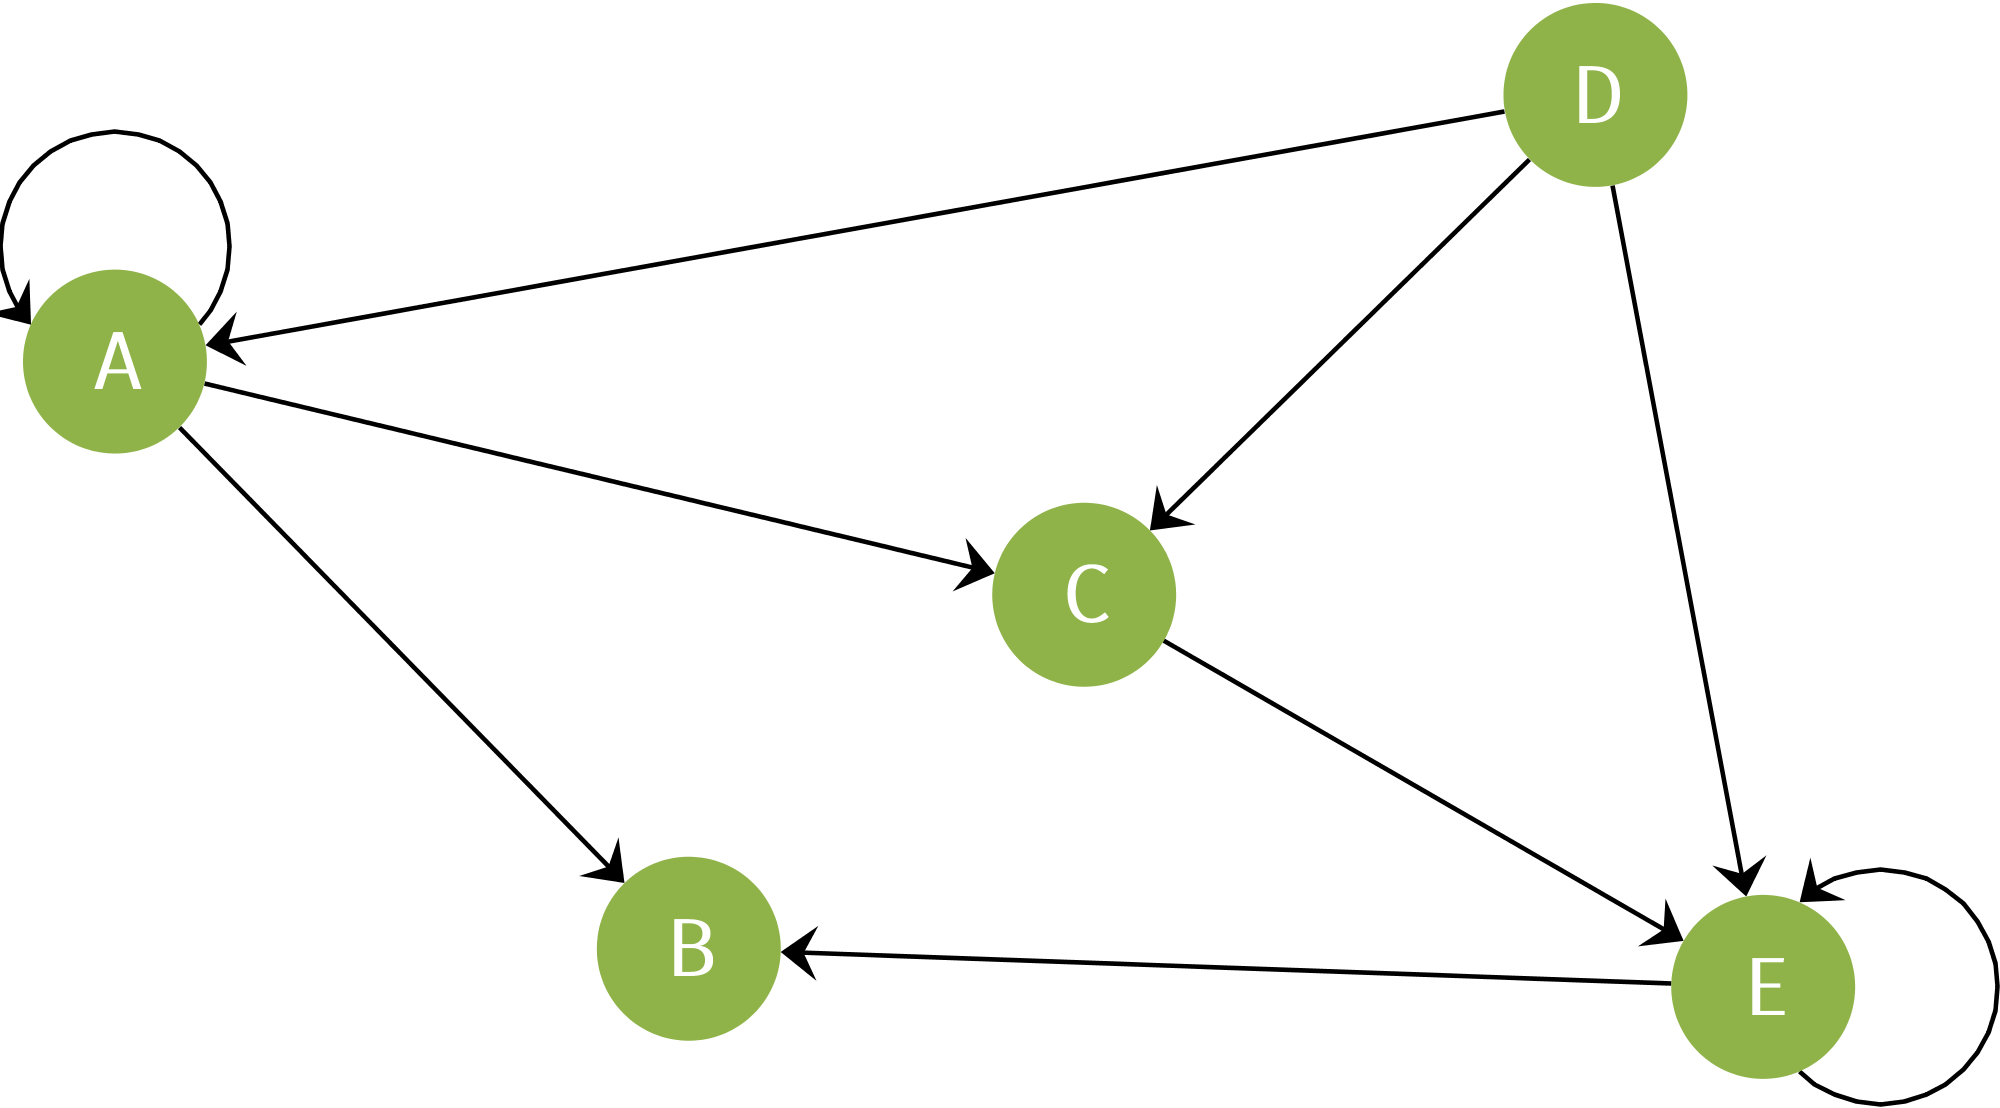
\includegraphics[width=7cm]{graphes/img/exo1_graphe1.png}\hspace*{2em}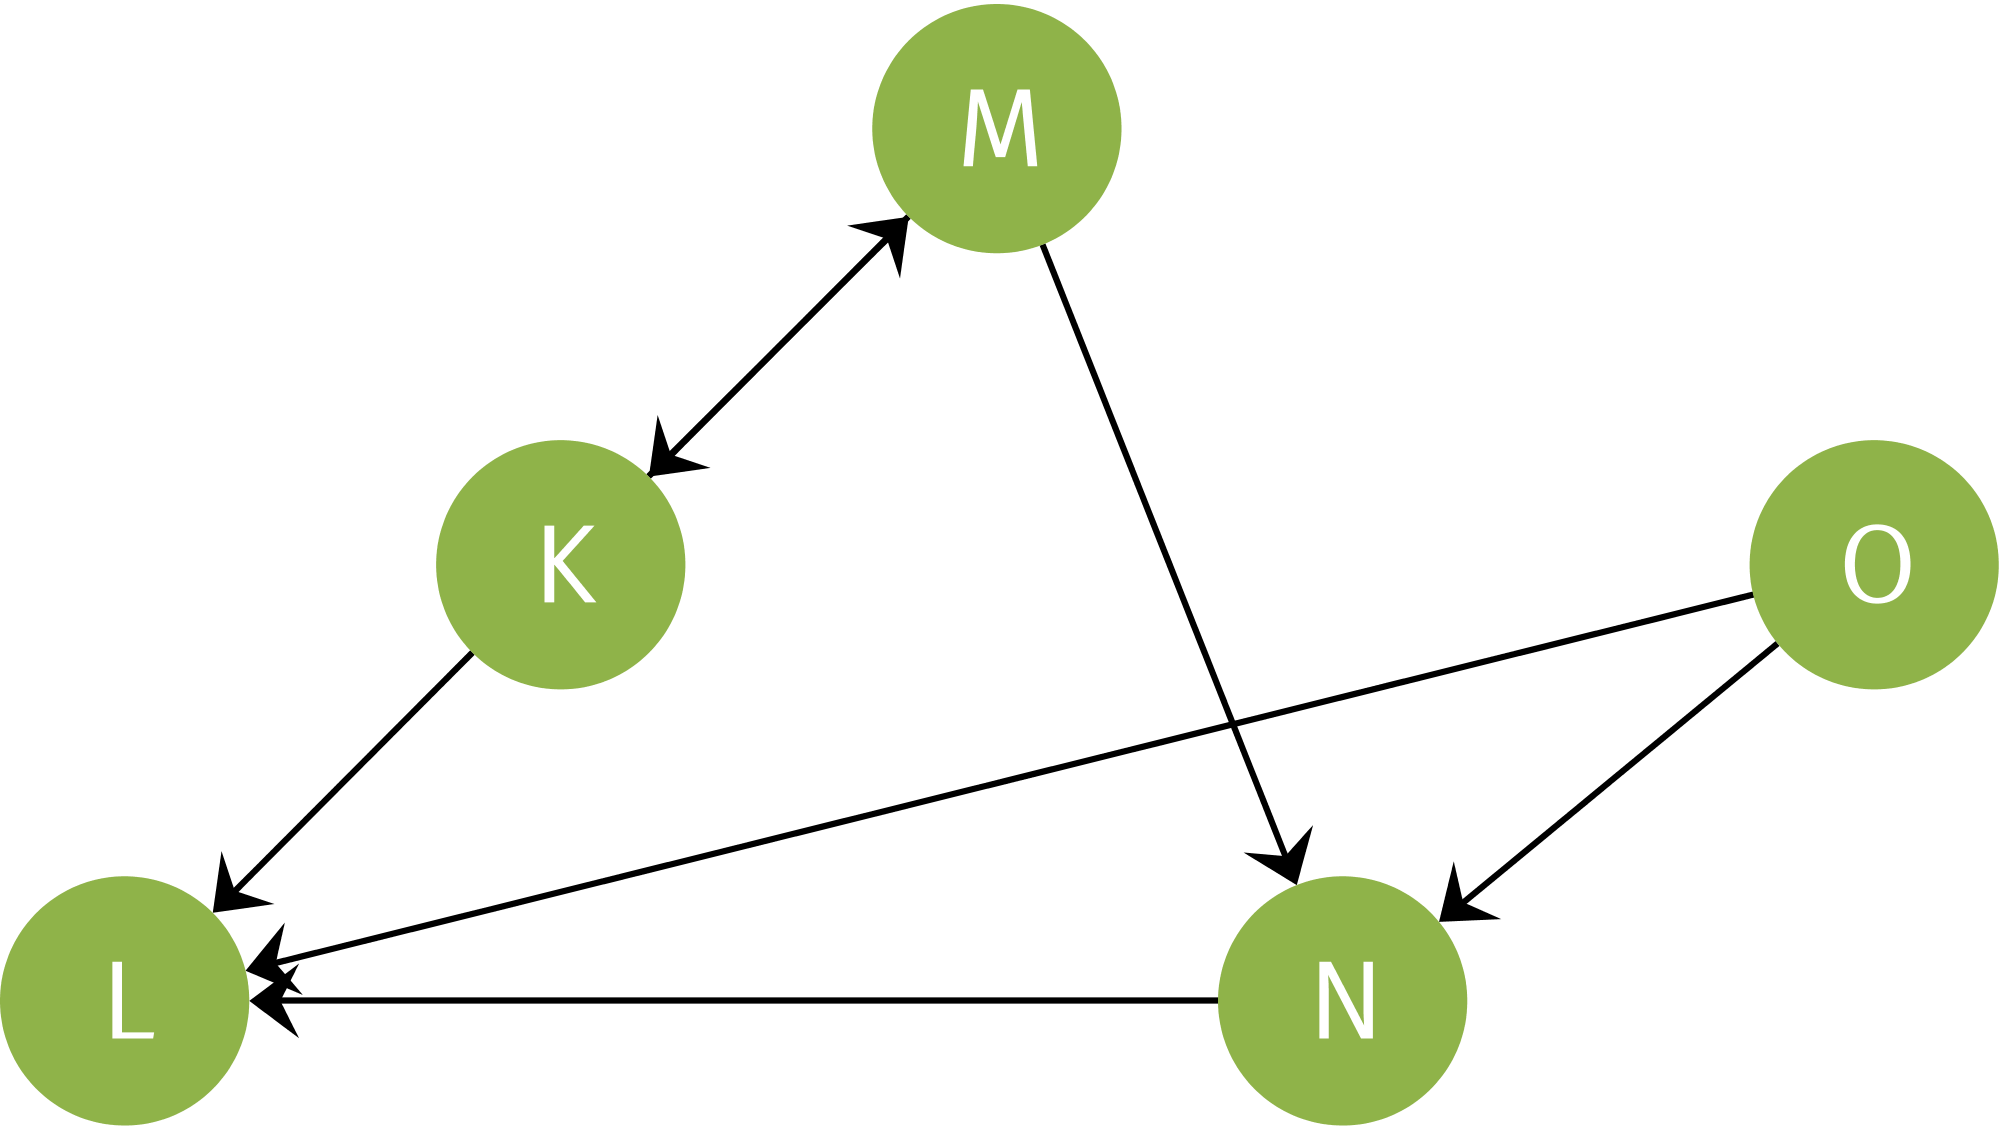
\includegraphics[width=6cm]{graphes/img/exo1_graphe2.png}
    \end{center}
\end{exercice}

\begin{exercice}[]
    Dessine le graphe correspondant au tableau de successeurs.
    \begin{center}
        \begin{tabular}{|c|c|c|c|c|}
            \hline
            \ccell sommet                            & \ccell A & \ccell B & \ccell C & \ccell D \\
            \hline
            \cellcolor{UGLiOrange}\ccell successeurs & A,B,C    & B,C,D    & C,D,A    & D,A,B    \\
            \hline
        \end{tabular}
    \end{center}
\end{exercice}

\begin{exercice}[]
    Dessine le graphe correspondant au tableau de prédécesseurs.
    \begin{center}
        \begin{tabular}{|c|c|c|c|c|c|}
            \hline
            \ccell sommet                              & \ccell A & \ccell B & \ccell C & \ccell D \\
            \hline
            \cellcolor{UGLiOrange}\ccell prédécesseurs & A,D      & ---      & A,B,D    & A        \\
            \hline
        \end{tabular}
    \end{center}
\end{exercice}

\subsection{Matrice d'adjacence}

\begin{definition}[ : matrice d'adjacence]
    Soit un graphe G de sommets  $S=\lbrace s_1;\,...;\,s_n\rbrace$ et d'arcs A. On appelle \textit{matrice d'adjacence de} G la matrice carrée d'ordre n $M=(m_{ij})$ telle que
    \begin{itemize}
        \item 	$m_{ij}=1$ s'il y a un arc partant de $s_i$ et arrivant sur $s_j$;
        \item 	$m_{ij}=0$ sinon.
    \end{itemize}
\end{definition}

\begin{exemple}[]
    En écrivant les sommets dans l'ordre alphabétique, la matrice d'adjacence du graphe ci-dessous est
    $$M=\begin{matrice}
            1 &1 &0 & 0&0  \\
            0 & 0&1 &0 &0  \\
            0 & \boxed{1} & 0 & 0 & 1\\
            1 & 0 & 1 & 0 & 1\\
            0 & 1 & 0 &{\color{red}1} & 0
        \end{matrice}$$
    \begin{center}
        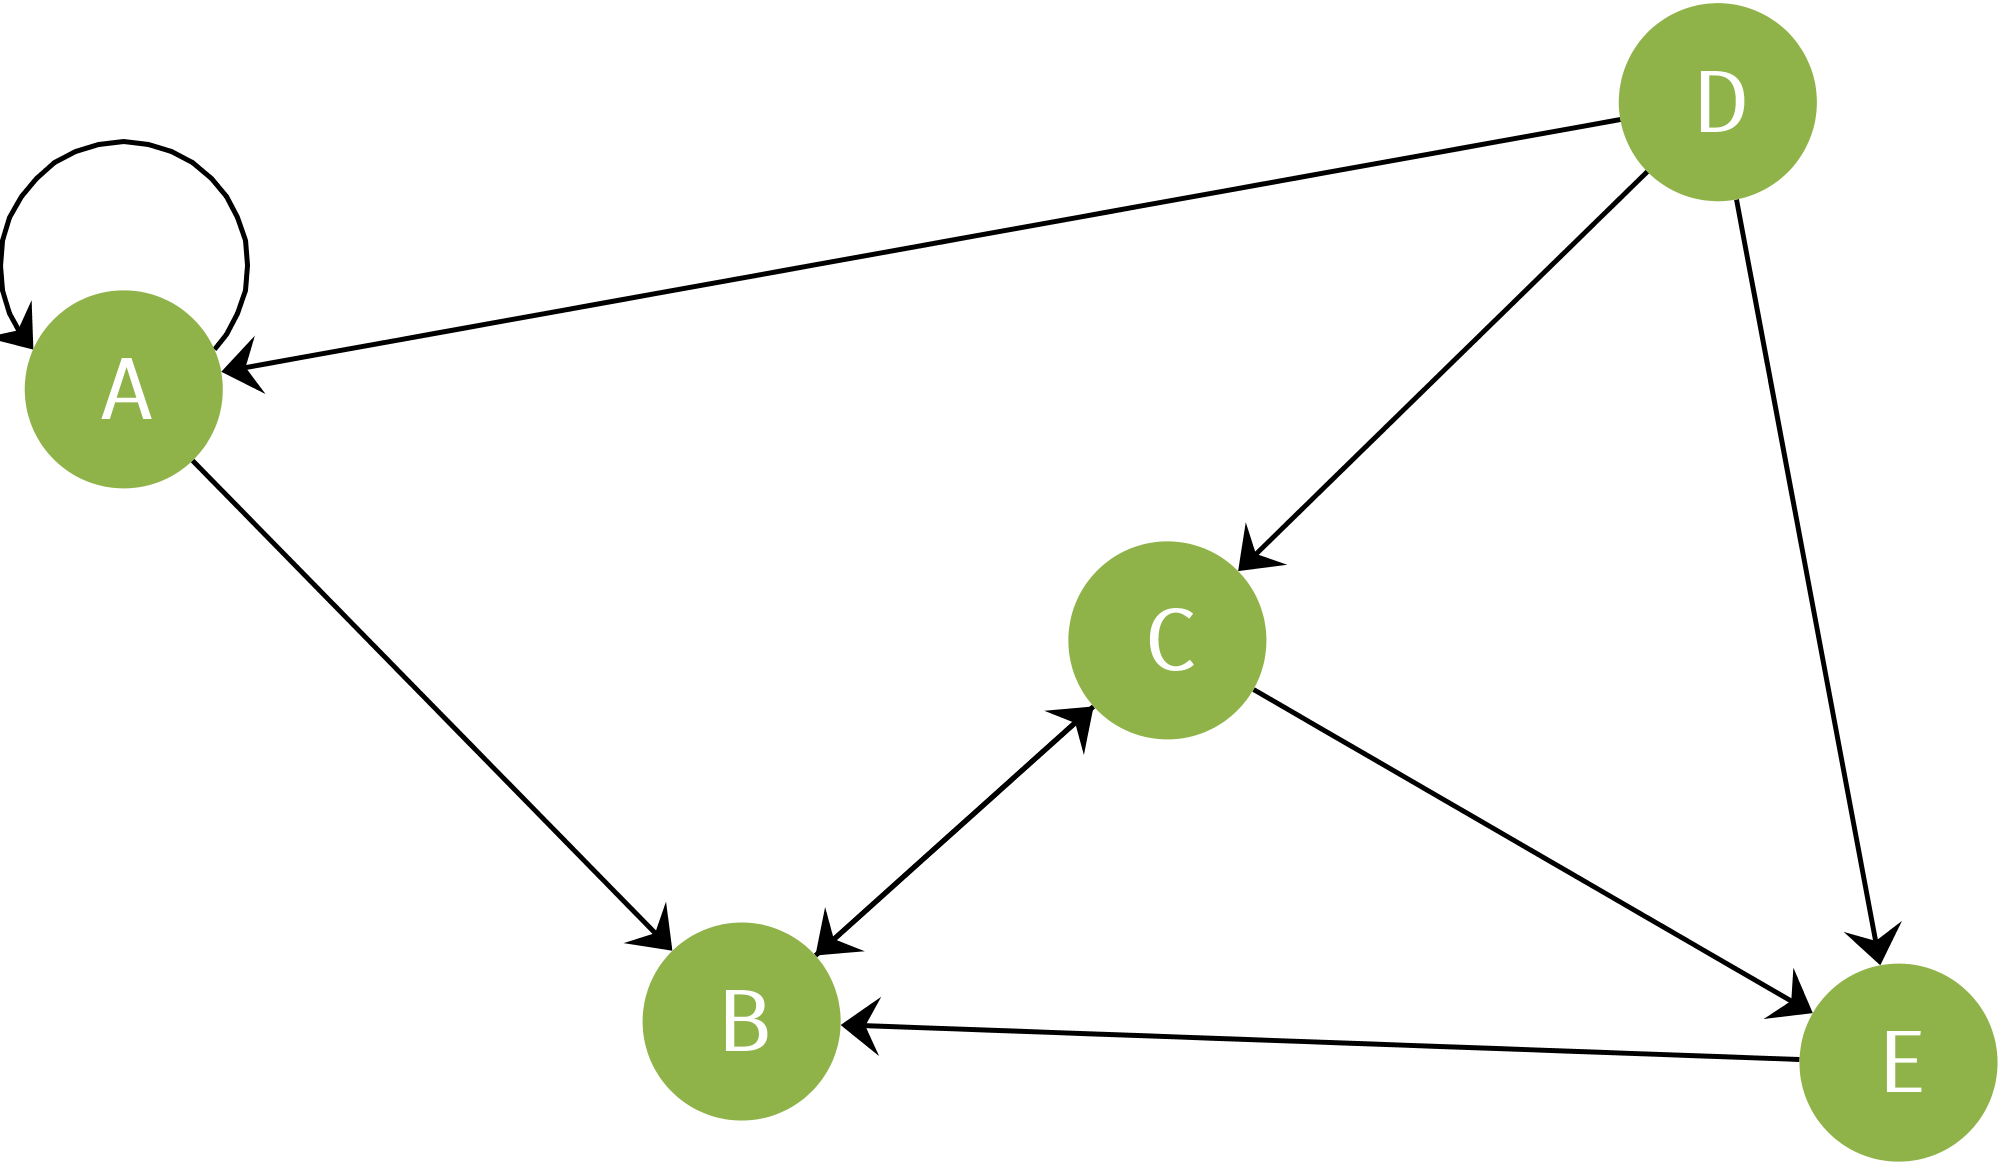
\includegraphics[width=6cm]{graphes/img/matr_adj1.png}
    \end{center}
    L'élément encadré de M est à la 3\eme ligne et à la 2\eme colonne : c'est $m32$. Il vaut 1 et signifie qu'il y a un arc partant du sommet 3, donc C, et allant au sommet 2, donc B.\\
    De même, du 5\eme sommet E, il existe un arc allant vers le 4\eme (D), donc $m_{54}=1$ (en rouge).
\end{exemple}

\begin{remarque}[]
    Dans une matrice d'adjacence
    \begin{itemize}
        \item 	Les lignes correspondent au points de départ, les colonnes au point d'arrivée;
        \item 	Sur une ligne donnée(la i\eme par exemple), on peut lire \textit{tous les successeurs} de $s_i$;
        \item 	Sur une colonne donnée, (la j\eme par exemple), on lite \textit{tous les prédécesseurs} de $s_j$;
    \end{itemize}
\end{remarque}

\begin{exercice}[]
    On considère un graphe dont l'ensemble des sommets est $\lbrace A;\,B;\,C;\,D;\,E;\,F\rbrace$, et dont la matrice d'adjacence est
    $$ M=\begin{matrice}
            1 &1 &0 & 1&0&1  \\
            0 & 0&0 &1 &0&1  \\
            1 & 0 & 0 & 0 & 1&1\\
            1 & 0 & 1 & 1 & 1&0\\
            0 & 1 & 0 &1 & 1 &1\\
            1 & 0 &1 & 0 &1& 0
        \end{matrice}$$
    
    \begin{enumerate}
        \item 	Donner le tableau des successeurs de chaque sommet.
        \item 	Donner le tableau des prédécesseurs de chaque sommet.
        \item 	Représenter ce graphe.
    \end{enumerate}
\end{exercice}

\section{Chemins et circuits}

\begin{definition}[s : chemin, longueur]
    
    On considère un graphe orienté.\\
    Un \textit{chemin} est une succession de sommets dans un ordre donné, chacun étant relié au suivant par un arc.\\
    La \textit{longueur} du chemin, c'est le nombre d'arcs qui composent le chemin. C'est aussi le nombre de sommets qui composent le chemin mois un.
\end{definition}

\begin{exemple}[]
    $(F,\,C,\,D,\,E)$ est un chemin de longueur 3.\\
    $(F,\,C,\,B,\,E)$ n'en est pas un car l'arc $(C,\,B)$ n'existe pas.
    \begin{center}
        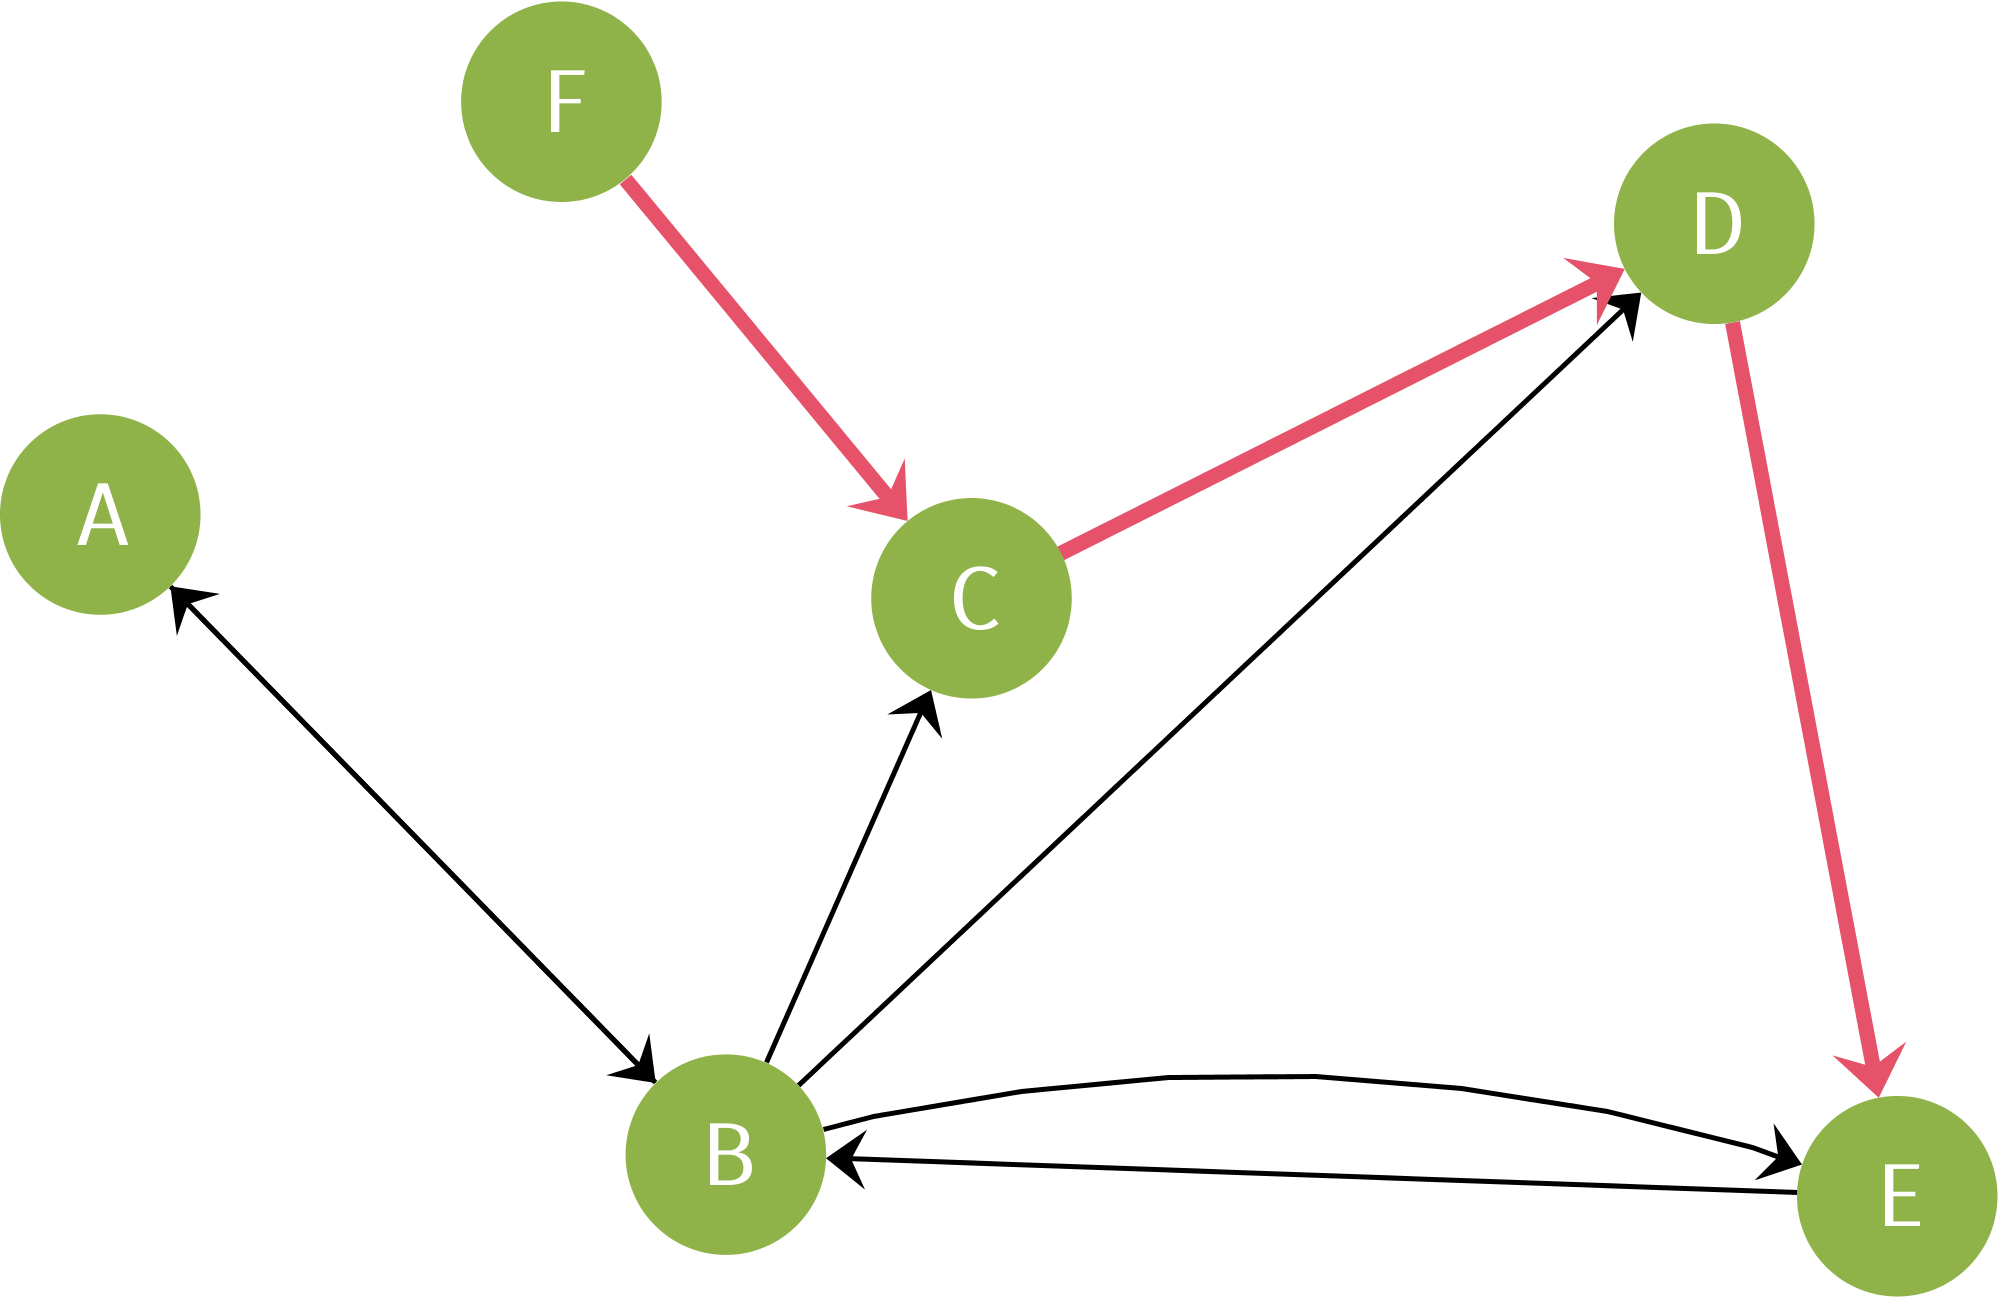
\includegraphics[width=7cm]{graphes/img/chemin.png}
    \end{center}
\end{exemple}

\begin{definition}[s : chemin hamiltonien,circuit]
    
    Un \textit{chemin hamiltonien} est un chemin qui passe une et une seule fois par \textit{chaque} sommet.\\
    Un \textit{circuit} est un chemin dont le premier et le dernier sommet sont identiques (un chemin  «  fermé »  en quelque sorte).
\end{definition}


\begin{exemple}[s]
    
    \begin{center}
        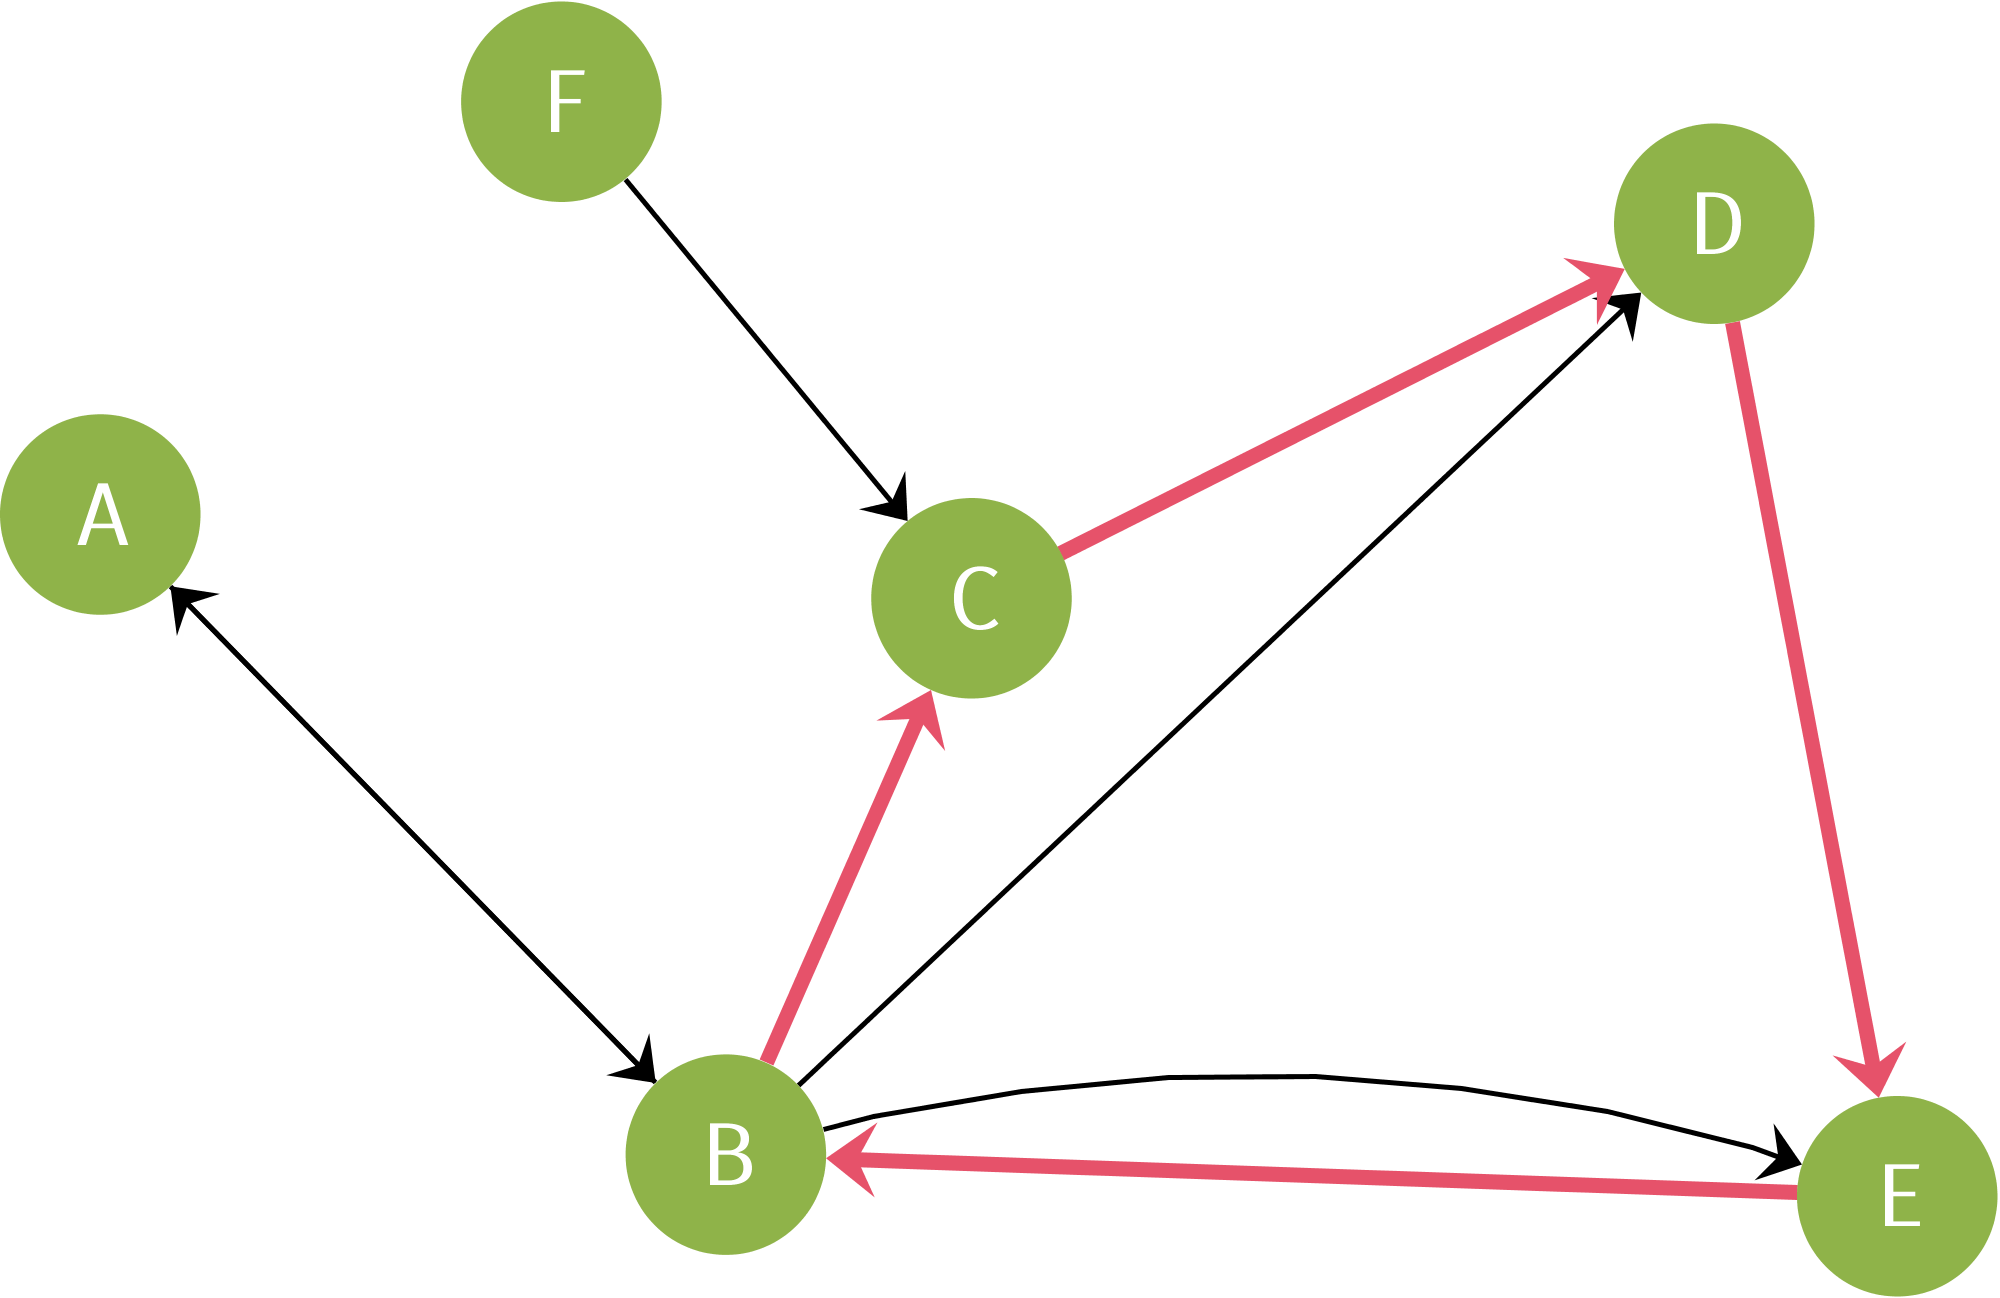
\includegraphics[width=7cm]{graphes/img/circuit.png}
    \end{center}
    $(C,\,D,\,E,\,B,\,C)$ est un circuit de longueur 4.
    
    \begin{center}
        \includegraphics[width=7cm]{graphes/img/chemin_hamiltonien.png}
    \end{center}
    $(F,\,C,\,D,\,E,\,B,\,A)$ est un chemin hamiltonien.
    
\end{exemple}

\begin{remarque}[]
    Un graphe orienté \textit{ne possède pas toujours} de circuit hamiltonien (à gauche) ou bien peut en posséder plusieurs (à droite).
    \begin{center}
        \includegraphics[width=4cm]{graphes/img/pas_de_ch.png}\hspace{2em}\includegraphics[width=4cm]{graphes/img/plusieurs_ch.png}
    \end{center}
\end{remarque}

\begin{exercice}[]
    Trouve un chemin hamiltonien, un circuit de longueur 3 et un autre de longueur 4.
    \begin{center}
        \includegraphics[width=7cm]{graphes/img/ex_circuit_ch.png}
    \end{center}
\end{exercice}

\section{Utilité des matrices d'adjacence}
On peut se poser beaucoup de questions ayant trait aux chemins d'un graphe. En voici trois que nous allons étudier :
\begin{itemize}
    \item 	On se donne un graphe à 10 sommets, on en choisit un en particulier. Combien de chemins différents de longueur 5 commencent en ce sommet ?
    \item 	Toujours dans ce graphe, combien y a-t-il de chemin de longueur 5 ?
    \item 	Si on veut (comme dans l'exemple introductif) ajouter tous les  «  raccourcis »  aux arcs du graphe, comment s'y prendre pour n'en oublier aucun ?
\end{itemize}



\begin{propriete}[]
    Soit $G$ un graphe possédant $n$ sommets $s_1$, $s_2$, \ldots $s_n$ et $M$ sa matrice d'adjacence.\\
    Soit $p$ un entier naturel positif. Alors $M^p$ contient les informations sur les chemins de longueur $p$ du graphe :
    
    Le nombre de chemins de longueur $p$ reliant $s_i$ à $s_j$ est le coefficient de la i\eme ligne et de la j\eme colonne de $M^p$.
\end{propriete}

\begin{exemple}[]
    La matrice d'adjacence du graphe ci-contre est
    $$M=\begin{matrice}
            0 & 1 & 0 & 0 & 1\\
            0 & 0 & 1 & 0 & 1\\
            0 & 0 & 0 & 1 & 0\\
            0 & 0 & 0 & 0 & 0\\
            0 & 0 & 0 & 1 & 0
        \end{matrice}$$
    Pour déterminer les chemins de longueur 3, calculons $M^3$ \textit{à l'aide de la calculatrice} :
    \begin{center}
        \includegraphics[width=5cm]{graphes/img/exemple_Mp.png}
        
        
        $M^3 = \begin{matrice}
                0 & 0 & 0 & 2 & 0\\
                0 & 0 & 0 & 0 & 0\\
                0 & 0 & 0 & 0 & 0\\
                0 & 0 & 0 & 0 & 0\\
                0 & 0 & 0 & 0 & 0\\
            \end{matrice}$
    \end{center}
    et le seul coefficient non nul est à la 1\ere ligne (départ A) et à la 3\eme colonne (arrivée D): il n'y a que 2 chemins de longueur 3 dans ce graphe, et ils relient $A$ à $D$.\\
    Maintenant qu'on connaît leur nombre et leurs extrémités, on peut les écrire : $(A,\,B,\,E,\,D)$ et $(A,\,B,\,C,\,D)$.
\end{exemple}

\begin{remarque}[]
    Ce procédé ne donne pas la liste des chemins de longueur donnée, seulement leur nombre et leurs extrémités.
\end{remarque}

\begin{exercice}[]
    On donne le tableau de prédécesseurs suivants :
    \begin{center}
        \tabstyled
        \begin{tabular}{c|c|c|c|c|c|c}
            \hline
            \ccell sommet                               & \ccell A & \ccell B & \ccell C & \ccell D & \ccell E & \ccell F \\
            \hline
            \cellcolor{UGLiOrange} \ccell prédécesseurs & ---      & ---      & A,B,E    & F        & B,D      & A,B      \\
            \hline
        \end{tabular}
    \end{center}
    En utilisant les puissances de la matrice d'adjacence :
    \begin{itemize}
        \item 	Donner tous les chemins de longueur 3.
        \item 	Montrer qu'il n'existe pas de chemin de longueur 4.
        \item 	Montrer que ce graphe ne possède pas de circuit.
    \end{itemize}
\end{exercice}

\section{Matrices booléennes et fermeture transitive}


Parfois on n'a pas besoin de connaître le nombre précis de chemins d'une longueur donnée reliant deux sommets. On veut juste savoir s'il en existe au moins un ou pas. Les matrices booléennes vont nous permettre de répondre simplement à cette question.\\

La matrice d'adjacence d'un graphe ne comporte que des zéros et des uns donc on peut la voir comme une \textit{matrice booléenne}, c'est à dire une matrice à coefficients dans l'algèbre de Boole $\mathcal{B}=\left\lbrace  0;\,1\right\rbrace$. Pour rappel, cette algèbre de Boole est munie des opérations binaires $+$ et $\times$ vérifiant :
\begin{itemize}
    \item 	$0+0 = 0$, $1+0 = 1$ et $1+1 = 1$ (penser au  «  ou »  logique)
    \item 	$0\times 0=0$, $1\times 0=0$ et $1\times 1 = 1$ (penser au  «  et »  logique)
\end{itemize}

\begin{definition}[s : addition et multiplication de matrices booléennes]
    Soient $A$ et $B$ 2 matrices booléennes.
    \begin{itemize}
        \item 	On définit $A\oplus B$, somme \textit{booléenne} de $A$ et de $B$ comme ceci : chaque coefficient de $A\oplus B$ est la somme booléenne des coefficients correspondants de $A$ et de $B$.\\
              En pratique on calcule $A+B$ comme d'habitude et on remplace chaque coefficient non nul par un 1.
        \item 	On définit $A\otimes B$, produit \textit{booléenne} de $A$ et de $B$ comme suit : on calcule $A\times B$ comme d'habitude et on remplace chaque coefficient non nul par un 1.
    \end{itemize}
\end{definition}
\begin{exemple}[s]
    
    Prenons $A=\begin{matrice}
            1 & 1 & 1 \\
            0 & 0 & 1 \\
            1 & 0 & 1 \\
        \end{matrice}$ et $B=\begin{matrice}
            0 & 1 & 0 \\
            1 & 0 & 1 \\
            1 & 0 & 1 \\
        \end{matrice}$.
    \begin{itemize}
        \item 	$A+B=\begin{matrice}
                      1 & 2 & 1 \\
                      1 & 0 & 2 \\
                      2 & 0 & 2 \\
                  \end{matrice}$ donc $A\oplus B=\begin{matrice}
                      1 & 1 & 1 \\
                      1 & 0 & 1 \\
                      1 & 0 & 1 \\
                  \end{matrice}$
        \item 	$A\times B =\begin{matrice}
                      2 & 1 & 2 \\
                      1 & 0 & 1 \\
                      1 & 1 & 1 \\
                  \end{matrice}$ donc $A\otimes B=\begin{matrice}
                      1 & 1 & 1 \\
                      1 & 0 & 1 \\
                      1 & 1 & 1 \\
                  \end{matrice}$
    \end{itemize}
\end{exemple}

\begin{definition}[ : puissance d'une matrice booléenne]
    
    Soit $A$ une matrice booléenne carrée de taille $n$.\\
    On pose $A^{[0]}=I_n$, $A^{[1]}=A$ et pour tout entier $p$ supérieur à 1:
    $$A^{[p]}=\underbrace{A\otimes\ldots \otimes A}_{p\text{\ facteurs}}$$
    En pratique il suffit de calculer $A^p$ et de remplacer les coefficients non nuls par des 1.
\end{definition}

\begin{exemple}[]
    Prenons $A =\begin{matrice}
            0 & 1 & 0\\1&0&1\\1&1&0
        \end{matrice}$ et $p=3$.\\
    Avec la calculatrice on obtient $A^3 =\begin{matrice}
            1 & 2 & 0\\2&1&2\\2&2&1
        \end{matrice}$ donc $A^{[3]} =\begin{matrice}
            1 & 1 & 0\\1&1&1\\1&1&1
        \end{matrice}$.\\
    
    Si $A$ est la matrice d'adjacence d'un graphe alors $A^{[3]}$ nous indique si 2 sommets du graphe peuvent être reliés ou non par un chemin de longueur 3 : on voit que c'est toujours possible sauf pour relier le 1\er au 3\eme.
\end{exemple}

On considère un graphe et on veut (comme dans l'exemple introductif) ajouter tous les  «  raccourcis »  aux arcs du graphe, comment s'y prendre pour n'en oublier aucun ?

Si notre graphe possède $n$ sommets, considérons 2 sommets $s_i$ et $s_j$, on veut rajouter l'arc $(s_i,\, s_j)$ (qu'on va appeler \textit{raccourci}) aux arcs du graphe dès qu'il existe un chemin allant de $s_i$ à $s_j$.\\
Nous allons admettre que c'est le cas si (et seulement si) il existe un chemin de longueur 1, ou 2, ..., ou $n-1$ qui relie ces 2 sommets. On arrive alors à la propriété et définition suivante :

\begin{propriete}[ et définition]
    Soit $M$ la matrice d'adjacence d'un graphe $G$ à $n$ sommets. On définit
    $$\widehat{M}=M\oplus M^{[2]}\oplus\ldots\oplus M^{[n-1]}$$
    
    $\widehat{M}$ est la matrice d'adjacence du graphe appelé \textit{fermeture transitive} de $G$, composé des mêmes sommets et arcs que ceux de $G$, auxquels on ajoute tous les arcs des  «  raccourcis » .
\end{propriete}

\begin{methode}[ : déterminer une fermeture transitive]
    On se donne le graphe ci-dessous, dont la matrice d'adjacence est
    
    $$M=\begin{matrice}0&0&1&1\\0&0&0&1\\0&1&0&0\\0&0&0&0\end{matrice}$$
    et on aimerait déterminer sa fermeture transitive.
    \begin{center}
        \includegraphics[width=4cm]{graphes/img/fermeture_transitive_0.png}
    \end{center}
    
    
    D'après la propriété précédente, étant donné que ce graphe possède 4 sommets on a $$\widehat{M}=M\oplus M^{[2]}\oplus M^{[3]}$$
    En pratique, on calcule $M^2$, $M^3$ puis $M+M^2+M^3$ et on remplace chaque coefficient non nul par un 1.\\
    Avec la calculatrice on obtient:
    $M^2=\begin{matrice}0&1&0&0\\0&0&0&0\\0&0&0&1\\0&0&0&0\end{matrice}$ et
    $M^3=\begin{matrice}0&0&0&1\\0&0&0&0\\0&0&0&0\\0&0&0&0\end{matrice}$ de sorte que
    $$M+M^2+M^3=\begin{matrice}0&1&1&2\\0&0&0&1\\0&1&0&1\\0&0&0&0\end{matrice}$$
    Donc en définitive $\widehat{M}=\begin{matrice}0&1&1&1\\0&0&0&1\\0&1&0&1\\0&0&0&0\end{matrice}$
    et on aboutit au graphe suivant :
    \begin{center}
        \includegraphics*[width=4cm]{graphes/img/fermeture_transitive_1.png}
    \end{center}
    où l'on a fait figurer en rouge les  «  raccourcis »  ajoutés. On peut remarquer que $M^3$ n'apporte pas grand-chose ici, car son seul coefficient non nul dit qu'il y a un chemin de longueur 3 : $(A,\,C,\,B,\,D)$ reliant $A$ et $D$, mais comme l'arc $(A,\,D)$ existe déjà,  «  le raccourci est déjà là » .
\end{methode}

\begin{exercice}[]
    Voici un graphe.
    \begin{center}
        \includegraphics[width=6cm]{graphes/img/exo_dm.png}
    \end{center}
    \begin{enumerate}
        \item 	Donner M, matrice d'adjacence du graphe.
        \item 	Calculer $\widehat{M}$, matrice de la fermeture transitive de ce graphe.
        \item 	Quels arcs doit-on ajouter au graphe ci-dessus pour réaliser sa fermeture transitive ?
    \end{enumerate}
\end{exercice}

\section{Exercices}
\begin{exercice}
    Cinq joueurs, notés A, B, C, D et E, jouent régulièrement à un jeu en ligne. Chaque partie de ce jeu oppose deux adversaires. Le tableau suivant donne, pour chacun des cinq joueurs, la liste des adversaires qu'il a déjà battus.
    \begin{center}
        \tabstyled
        \begin{tabular}{c|c}\hline
            \ccell Le joueur & \ccell a déjà battu \\ \hline
            A                & B, D                \\ \hline
            B                & C                   \\ \hline
            C                & B, D                \\ \hline
            D                & E                   \\ \hline
            E                & D                   \\ \hline
        \end{tabular}
    \end{center}
    Ainsi, par exemple, le joueur C a déjà battu les joueurs B et D.
    \begin{enumerate}
        \item Graphe orienté associé à la situation
              \begin{enumalph}
                  \item En considérant le tableau précédent comme un tableau de successeurs, représenter la
                  situation par un graphe orienté $G$, dans lequel un arc relie un sommet $x$ à un sommet $y$ si le
                  joueur $x$ a déjà battu le joueur $y$.
                  \item Écrire la matrice d'adjacence $M$ du graphe $G$.
                  \item Recopier et compléter le tableau des \textbf{prédécesseurs} dans le graphe $G$.
                  \begin{center}
                    \tabstyled
                      \begin{tabular}{c|c}\hline
                          \ccell Le joueur & \ccell a déjà \ldots \\ \hline
                          A                &                        \\ \hline
                          B                &                        \\ \hline
                          C                &                        \\ \hline
                          D                &                        \\ \hline
                          E                &                        \\ \hline
                      \end{tabular}
                  \end{center}
                  \item Le graphe $G$ contient-il un circuit ? Contient-il un chemin hamiltonien ? Justifier les
                  réponses.
              \end{enumalph}
    \end{enumerate}
\end{exercice}

\begin{exercice}
    Un fournisseur doit livrer 5 entreprises. Le réseau de transport est représenté par le graphe orienté
    donné ci-dessous où l'entrepôt du fournisseur est noté $F$, et les entreprises sont notées $A$, $B$, $C$, $D$, $E$.
    
    \begin{center}
        \includegraphics[width=5cm]{graphes/img/g2.png}
    \end{center}
    
    \begin{enumerate}
        \item Écrire la matrice d'adjacence $M$ de ce graphe en considérant les sommets notés $A$, $B$, $C$, $D$, $E$, et $F$ dans cet ordre.
        \item  Le fournisseur souhaite livrer chacune des entreprises. Il part de son entrepôt.
              \begin{enumalph}
                  \item Existe-t-il un chemin hamiltonien d'origine $F$ dans ce graphe ? Si oui, citer un tel chemin.
                  \item Interpréter le résultat relativement aux possibilités de livraison.
              \end{enumalph}
        \item  On donne la matrice $M^3 = \begin{matrice}
                      1& 1& 0	& 1	& 0	&0\\
                      2& 0& 4 & 0	&1	&3\\
                      1& 3& 0 & 3	&1	&0\\
                      1&0	&2	& 0	&0	&1\\
                      1&0	& 2	& 0	&1	&1\\
                      1&3	& 0	& 3	&1	&1 \end{matrice}$.
              \begin{enumalph}
                  \item Dans le contexte de l'exercice, interpréter le coefficient 2 situé sur la quatrième ligne et la troisième colonne de la matrice $M^3$.
                  \item Combien existe-t-il de chemins de longueur 3 issus du sommet $D$ dans ce graphe ? Justifier puis citer ces chemins.
                  \item Le fournisseur doit maintenant effectuer une livraison, depuis l'entrepôt, dans quatre
                  entreprises en commençant par l'entreprise $D$.
                  
                  Montrer que, pour effectuer cette livraison sans repasser par une entreprise déjà livrée, le
                  fournisseur n'a qu'un seul chemin possible.
                  
                  Expliquer la démarche et préciser ce chemin.
              \end{enumalph}
    \end{enumerate}
\end{exercice}

\begin{exercice}
    \textbf{Partie A}\\
    \medskip
    Quatre sites internet traitent les changements climatiques et leurs conséquences sur la planète. On
    considère une page web sur chacun de ces sites, et on note ces quatre pages A, B, C et D. Les liens
    hypertextes respectifs entre ces quatre pages sont tous récapitulés dans l'énumération suivante:
    \begin{itemize}
        \item A reçoit un unique lien de B et un unique lien de C ;
        \item B reçoit un unique lien de D ;
        \item C reçoit un unique lien de B, un unique lien de D et un unique lien de A ;
        \item D reçoit un unique lien de A.
    \end{itemize}
    \begin{enumerate}
        \item Représenter l'ensemble de ces liens par un graphe orienté $G$ de sommets A, B, C, D, dans lequel,
              si une page $Y$ reçoit un lien d'une page $X$, on représente un arc du sommet $X$ vers le sommet $Y$.
        \item
              \begin{enumalph}
                  \item Donner la matrice d'adjacence $M$ du graphe $G$.
                  \item Interpréter les valeurs des termes situés sur la diagonale de la matrice $M$.
                  \item Calculer la matrice $M^4$.
                  \item Le graphe contient-il des circuits ? Justifier la réponse.
                  \item Interpréter le terme de la 1\ere et  3\eme colonne  de la matrice $M^4$ en termes de chemins, puis donner la liste de ces chemins.
              \end{enumalph}
        \item Calculer $\hat{M}$, la matrice de la fermeture transitive du graphe $G$.\\
              Interpréter le résultat obtenu dans le contexte de l'exercice.
    \end{enumerate}
    \bigskip
    \textbf{Partie B}\\
    \medskip
    Un étudiant du BTS SIO a mis en place un moteur de recherche avec lequel les pages affichées sont
    ordonnées par pertinence, selon le nombre de liens hypertextes pointant vers chaque page.\\
    Cette partie étudie un exemple simplifié, en limitant ce moteur de recherche aux quatre pages web
    A, B, C et D définies dans la partie A, et en considérant le graphe associé $G$.\\
    La méthode mise en place par l'étudiant consiste à associer un score à chaque sommet du graphe.\\
    Les scores $a$, $b$, $c$, $d$ de chacun des sommets A, B, C, D, sont calculés à partir des instructions
    suivantes :
    \begin{itemize}
        \item on liste les prédécesseurs du sommet considéré dans le graphe $G$ ;
        \item on divise le score de chaque prédécesseur par le nombre de ses successeurs;
        \item le score d'un sommet est obtenu en ajoutant les quotients obtenus.
    \end{itemize}
    \emph{Exemple }: le sommet A possède deux prédécesseurs B et C ; B a 2 successeurs et C a 1 successeur.\\
    D'où $a = \dfrac{b}{2} + \dfrac{c}{1}$.
    
    \medskip
    
    \begin{enumerate}
        \item Justifier l'égalité : $c = \dfrac{a}{2} + \dfrac{b}{2} + \dfrac{d}{2}$.
              
        \item  En établissant les quatre égalités vérifiées par les scores $a$, $b$, $c$, $d$, on obtient un système de quatre équations linéaires aux inconnues $a$, $b$, $c$, $d$. Ce système ayant une infinité de solutions,
              toutes proportionnelles entre elles, on pose $a = 1$ et on admet que la résolution se ramène à celle
              du système :
              
              \[(S) \quad \left\lbrace \begin{array}{l c r}
                      0,5b + c                              & = & 1     \\
                      \phantom{0,5} b \phantom{+ c } - 0,5d & = & 0     \\
                      0,5b - c + 0,5d                       & = & - 0,5
                  \end{array}\right.\]
              
              On définit les matrices $X = \begin{matrice}b\\c\\d\end{matrice}$,\quad  $A = \begin{matrice}0,5&1&0\\1&0&-0,5\\0,5&- 1&0,5
                  \end{matrice}$  \\et $B = \begin{matrice}0,5 &0,5& 0,5\\0,75& - 0,25&- 0,25\\1&- 1&1\end{matrice}$.
              \begin{enumalph}
                  \item Exprimer le système $(S)$ sous la forme $A \times X = Y$, où $Y$ est une matrice à préciser.
                  \item Calculer le produit $B \times A$.
                  \item En déduire que $X = B \times Y$, puis donner la solution du système $(S)$.
              \end{enumalph}
        \item  Donner, en justifiant, le classement des pages web A, B, C et D selon la méthode mise en place.
    \end{enumerate}
\end{exercice}
\chapter{Graphes : méthodes et algorithmes}

\section{Niveaux dans un graphe orienté sans circuit}

On dit qu'un graphe orienté est \textit{sans circuit} lorsqu'il \dots ne comporte aucun circuit, c'est-à-dire qu'on ne peut pas trouver un chemin partant d'un sommet et y revenant.


\begin{multicols}{2}
    \begin{center}
        \includegraphics[width=7cm]{graphes2/img/graphe_sans_circuit.png}\\ \footnotesize graphe sans circuit\\
        \includegraphics[width=7cm]{graphes2/img/graphe_avec_circuit.png}\\ \footnotesize graphe avec circuit
    \end{center}
\end{multicols}

Lorsqu'un graphe orienté est sans circuit il est possible de l'organiser de manière \textit{hiérarchisée}, comme ceci :
\begin{multicols}{2}
    \begin{center}
        \includegraphics[width=7cm]{graphes2/img/graphe_sans_circuit_non_hierarchise.png}\\ \footnotesize graphe sans circuit\\
        \includegraphics[width=5cm]{graphes2/img/graphe_sans_circuit_hierarchise.png}\\ \footnotesize le même graphe  hiérarchisé
    \end{center}
\end{multicols}

Comment faire ? À droite, on voit que les sommets sont disposés en couches horizontales : des \textit{niveaux}. Il faut donc définir ce qu'est le niveau d'un sommet.

\begin{propriete}[]
    Dans un graphe orienté sans circuit, il existe un sommet qui n'a pas de prédécesseur.
\end{propriete}
\begin{encadrecolore}{Preuve}{gray}
    Soit $n$ le nombre de sommets du graphe. On va raisonner par l'absurde : supposons que notre graphe soit sans circuit, mais qu'il n'existe aucun sommet sans prédécesseur. Alors tout sommet possède un prédécesseur.\\
    On en choisit un, on l'appelle  $S_0$ puis un de ses prédécesseurs qu' on appelle $S_1$
    \begin{itemize}
        \item 	si $S_1=S_0$ alors il y a une boucle (donc un circuit de longueur 1) sur $S_0$ et c'est contradictoire avec notre hypothèse.
        \item 	sinon on continue et on appelle $S_2$ un prédécesseur de $S_1$.
    \end{itemize}
    À chaque nouveau sommet choisi si c'est un sommet qui figure déjà dans la liste des sommets choisis, cela nous permet d'exhiber un circuit et c'est contradictoire. Or comme il n'y a que $n$ sommets, au bout de $n$ étapes (au maximum), on sera obligés de choisir un sommet déjà choisi.
\end{encadrecolore}


\begin{definition}[ : niveau d'un sommet dans un graphe orienté sans circuit]
    Soit un sommet d'un graphe orienté sans circuit
    \begin{itemize}
        \item 	s'il n'a pas de prédécesseur, son niveau est 0;
        \item 	sinon, on considère tous ses prédécesseurs, on choisit celui qui a le niveau le plus élevé et on ajoute 1 : on obtient le niveau du sommet.
    \end{itemize}
\end{definition}

Pour déterminer les niveaux des sommets on peut aussi appliquer l'algorithme suivant :
\begin{verbatim}
Variables
    L : liste des sommets
    n : entier 
Début
    n <-- 0
    tant que L est non vide
        sélectionner tous les sommets qui n'ont aucun prédécesseur dans L
        ils ont le niveau n
        enlever ces sommets de L
	    n <-- n + 1
Fin
\end{verbatim}


\begin{exemple}[]
    On considère le graphe suivant :
    \begin{center}
        \includegraphics[width=7cm]{graphes2/img/nivellement_exemple.png}
    \end{center}
    On commence par construire le tableau des prédécesseurs :\\

    \def\ltb{.6cm}
    \tabstyled
    \begin{tabular}{|l|>{\centering\arraybackslash}m{\ltb}|>{\centering\arraybackslash}m{\ltb}|>{\centering\arraybackslash}m{\ltb}|>{\centering\arraybackslash}m{\ltb}|>{\centering\arraybackslash}m{\ltb}|>{\centering\arraybackslash}m{\ltb}|>{\centering\arraybackslash}m{\ltb}|>{\centering\arraybackslash}m{\ltb}|>{\centering\arraybackslash}m{\ltb}|>{\centering\arraybackslash}m{\ltb}|>{\centering\arraybackslash}m{\ltb}|}
        \hline
        \ccell sommet        & A & Z   & E & R   & T     & Y   & U   & I & O   & P     & Q \\
        \hline
        \ccell prédécesseurs & E & A,E & O & --- & R,E,Y & E,O & Y,I & O & --- & I,O,Q & O \\
        \hline
    \end{tabular}\\

    R et O ont le niveau 0. On les retire du tableau :\\

    \tabstyled
    \begin{tabular}{|l|>{\centering\arraybackslash}m{\ltb}|>{\centering\arraybackslash}m{\ltb}|>{\centering\arraybackslash}m{\ltb}|>{\centering\arraybackslash}m{\ltb}|>{\centering\arraybackslash}m{\ltb}|>{\centering\arraybackslash}m{\ltb}|>{\centering\arraybackslash}m{\ltb}|>{\centering\arraybackslash}m{\ltb}|>{\centering\arraybackslash}m{\ltb}|}
        \hline
        \ccell sommet        & A & Z   & E   & T   & Y & U   & I   & P   & Q   \\
        \hline
        \ccell prédécesseurs & E & A,E & --- & E,Y & E & Y,I & --- & I,Q & --- \\
        \hline
    \end{tabular}\\

    E, I et Q ont le niveau 1, on les retire :\\
    \tabstyled
    \begin{tabular}{|l|>{\centering\arraybackslash}m{\ltb}|>{\centering\arraybackslash}m{\ltb}|>{\centering\arraybackslash}m{\ltb}|>{\centering\arraybackslash}m{\ltb}|>{\centering\arraybackslash}m{\ltb}|>{\centering\arraybackslash}m{\ltb}|}
        \hline
        \ccell sommet        & A   & Z & T & Y   & U & P   \\
        \hline
        \ccell prédécesseurs & --- & A & Y & --- & Y & --- \\
        \hline
    \end{tabular}\\

    A, Y et P ont le niveau 2 et on voit que Z, T et U ont le niveau 3.\\

    \tabstyled
    \def\ltb{.75cm}
    \begin{tabular}{|l|>{\centering\arraybackslash}m{\ltb}|>{\centering\arraybackslash}m{\ltb}|>{\centering\arraybackslash}m{\ltb}|>{\centering\arraybackslash}m{\ltb}|>{\centering\arraybackslash}m{\ltb}|>{\centering\arraybackslash}m{\ltb}|>{\centering\arraybackslash}m{\ltb}|>{\centering\arraybackslash}m{\ltb}|>{\centering\arraybackslash}m{\ltb}|>{\centering\arraybackslash}m{\ltb}|>{\centering\arraybackslash}m{\ltb}|}
        \hline
        \ccell sommet & R & O & E & I & Q & A & Y & P & Z & T & U \\
        \hline
        \ccell niveau & 0 & 0 & 1 & 1 & 1 & 2 & 2 & 2 & 3 & 3 & 3 \\
        \hline
    \end{tabular}\\

    On peut maintenant redessiner le graphe de manière hiérarchisée de haut en bas ou de droite à gauche, en alignant les sommets par niveaux :

    \begin{center}
        \includegraphics[width=10cm]{graphes2/img/nivellement_exemple_fait.png}\\ {\footnotesize graphe représenté de manière nivelée}

    \end{center}
\end{exemple}

En appliquant cette méthode on peut parfois prouver qu'un graphe donné est une \textit{arborescence}.

\begin{definition}[ : arborescence]
    Une \textit{arborescence} est un graphe oriente qui possède \textit{un unique sommet de niveau 0}, qu'on appelle la \textit{racine} et à partir de laquelle on peut atteindre \textit{tout autre sommet par un unique chemin}.
    \begin{multicols}{2}
        \begin{center}
            \includegraphics[width=7cm]{graphes2/img/ex_arborescence.png}\\ \footnotesize graphe qui est une arborescence\\
            \includegraphics[width=7cm]{graphes2/img/ex_pas_arborescence.png}\\ \footnotesize graphe qui n'en est pas une
        \end{center}
    \end{multicols}
\end{definition}
\begin{exercice}[]
    \begin{center}
        \includegraphics[width=7cm]{graphes2/img/exo_niveau_1.png}
    \end{center}
    \begin{enumerate}
        \item 	Dresser le tableau des prédécesseurs du graphe ci-dessus.
        \item 	Déterminer le niveau de chaque sommet.
        \item 	Dessiner le graphe de manière hiérarchisée.
        \item 	Ce graphe est-il une arborescence ?
    \end{enumerate}
\end{exercice}

\begin{exercice}[]
    \begin{center}
        \includegraphics[width=6cm]{graphes2/img/exo_niveau_2.png}
    \end{center}
    Même consigne.
\end{exercice}

\begin{exercice}[]
    \begin{center}
        \includegraphics[width=7cm]{graphes2/img/exo_niveau_3.png}
    \end{center}
    Même consigne.
\end{exercice}
\section{Graphes orientés valués et ordonnancement}


\begin{definition}[ : graphe orienté valué]
    un graphe orienté est dit \textit{valué} (on dit aussi pondéré) lorsqu'on attribue un nombre réel à chacun de ses arcs.
    \begin{center}
        \includegraphics[width=7cm]{graphes2/img/graphe_value.png}\\un exemple de graphe valué
    \end{center}
\end{definition}

Imaginons maintenant une équipe de plusieurs personnes qui travaille sur un projet, (ce peut être le développement d'une application ou bien la construction d'une salle de sport). Toutes les personnes ne travaillent pas sur les mêmes aspects du projet. Certaines tâches peuvent être réalisées en même temps (par exemple on peut penser qu'on peut poser un revêtement au sol de la salle de sport en même temps qu'on peint sa façade). Certaines doivent attendre que d'autres soient terminées pour pouvoir commencer (évidemment avant de peindre la façade il faut avoir monté la façade), on parle de \textit{contraintes d'antériorité}.\\
Les contraintes d'antériorité conduisent naturellement à un graphe orienté. Chaque tâche possède une durée propre, qui conduit à pondérer le graphe.\\

\textit{Faire de l'ordonnancement}, c'est préciser la chronologie des différentes tâches (éventuellement effectuées en parallèle), déterminer la durée minimale du projet et les conséquences éventuelles d'un retard lors de la réalisation de telle ou telle tâche.

\subsection*{La méthode MPM sur un exemple}

Cette méthode de gestion de projet, appelée méthode des potentiels métra (MPM) fut développée par le mathématicien français Bernard Roy en 1958, pour être directement appliquée en usine.\\

On va considérer le tableau de tâches suivant

\begin{center}
    \tabstyle
    \begin{tabular}{lccccccc}
        \hline
        \ccell Tâche              & A   & B   & C   & D & E & F    & G       \\
        \hline
        \ccell Durée en jours     & 6   & 3   & 6   & 2 & 4 & 3    & 1       \\
        \hline
        \ccell Tâches antérieures & --- & --- & --- & B & B & A, D & C, E, F \\
        \hline
    \end{tabular}\\
\end{center}
Dans celui-ci on lit, par exemple, que la tâche F dure 3 jours et ne peut commencer que lorsque A et D sont terminées.\\


Cet exemple va nous servir à illustrer la méthode MPM, mais nous donnerons les définitions dans le cas général.

\begin{encadrecolore}{Notations}{UGLiPurple}
    On note $G$ le graphe orienté valué qui représente les tâches du projet.\\
    Il a $n$ sommets $s_1$, ..., $s_n$ qui représentent toutes les tâches. On écrit $s_i$ pour parler d'un de ces sommets sans dire précisément lequel.\\
    On note aussi $d(s_i)$ la durée de la tâche $s_i$, c'est la valeur (le poids) de tous les arcs qui partent de $s_i$.
\end{encadrecolore}



\subsubsection*{Niveler le graphe}

Dans le graphe qu'on va construire, les tâches antérieures sont les \textit{prédécesseurs directs} de chaque tâche, et il n'y a pas de circuit (heureusement pour le projet). On peut donc niveler le graphe :
\begin{itemize}
    \item 	A, B et C sont clairement de niveau 0;
    \item 	D et E sont de niveau 1;
    \item 	F est de niveau 2;
    \item 	G est de niveau 3.
\end{itemize}
Cela nous permet de représenter le graphe du projet de manière hiérarchisée. On parle alors de \textit{graphe d'ordonnancement}. Pour les besoins on rajoute 2 sommets « fictifs»{} : le début et la fin du projet. On pondère les arcs par les durées des tâches (on met 0 en partant de début car on considère que le projet peut commencer maintenant) :
\begin{center}
    \includegraphics[width=12cm]{graphes2/img/exemple_mpm0.png}
\end{center}
Puis, étant donné que l'on va déterminer beaucoup de paramètres, on utilisera plutôt cette représentation :
\begin{center}
    \includegraphics[width=\linewidth]{graphes2/img/exemple_mpm1.png}
\end{center}
Comme on peut le voir, pour chaque sommet, on peut déterminer 5 paramètres :\\

\dleft{4cm}{\includegraphics[width=4cm]{graphes2/img/sommet_template.png}}{\begin{enumerate}
        \item 	D'abord, on détermine la \textit{date au plus tôt} de chaque tâche.
        \item 	Ensuite on peut déterminer la \textit{date au plus tard} de chaque tâche.
        \item 	Cela permet de déterminer la \textit{marge totale} de chaque tâche, ainsi que la \textit{marge libre} et la \textit{marge certaine}.
    \end{enumerate}Nous allons définir ces nombres au fur et à mesure.}

\subsubsection*{Date au plus tôt}

\begin{definition}[ : date au plus tôt]
    On note $t(s_i)$ la \textit{date au plus tôt} de la tâche $s_i$. Puisque $s_i$ ne peut commencer que lorsque toutes les tâches antérieures sont terminées on a
    $$t(s_i)=\max\left(\left\{t(s_j)+d(s_j)\::\:s_j\,\text{ prédécesseur de }\:s_i\right\}\right)$$
\end{definition}
\begin{exemple}[]
    \begin{center}
        \includegraphics[width=5.5cm]{graphes2/img/mpm_au_plus_tot.png}
    \end{center}
    Pour calculer la date au plus tôt de $s_8$, il faut que les tâches antérieures $s_2$, $s_4$ et $s_5$ soient terminées :
    \begin{itemize}
        \item 	$s_2$ commence au bout de 10 jours, dure 4 jours, donc est terminée au bout de 14 jours;
        \item 	$s_4$ commence au bout de 12 jours, dure 3 jours, donc est terminée au bout de 15 jours;
        \item 	$s_5$ commence au bout de 4 jours,  dure 10 jours, donc est terminée au bout de 14 jours.
    \end{itemize}
    En définitive, $t(s_8)=15$.
\end{exemple}

Calculons toutes les dates au plus tôt de notre projet. On commence par le début et on procède \textit{niveau par niveau} dans l'ordre hiérarchique :
\begin{center}
    \includegraphics[width=\linewidth]{graphes2/img/exemple_mpm2.png}
\end{center}
\begin{definition}[ : durée minimale de réalisation d'un projet]
    C'est le temps minimal requis pour que toutes les tâches soient accomplies en respectant les contraintes.
\end{definition}
Dans notre cas la \textit{durée minimale du projet} est de 10 jours.

\subsubsection*{Date au plus tard}

\begin{definition}[ : date au plus tard]
    On note $T(s_i)$ la \textit{date au plus tard} de la tâche $s_i$ : c'est la date maximale à laquelle on peut commencer $s_i$ sans que cela ne repousse la date de fin du projet.
    $$T(s_i)=\min\left(\left\{T(s_j)-d(s_i)\::\:s_j\,\text{ successeur de }\:s_i\right\}\right)$$
\end{definition}
\begin{exemple}[]
    \begin{center}
        \includegraphics[width=5.5cm]{graphes2/img/mpm_au_plus_tard.png}
    \end{center}
    On n'a pas renseigné les dates au plus tôt car elles n'interviennent pas ici, mais normalement elles doivent avoir été calculées d'abord.\\
    La tâche $s_4$ dure 6 jours
    \begin{itemize}
        \item 	puisqu'on peut commencer $s_5$ au plus tard au bout de 20 jours, il faut commencer $s_4$ au plus tard au bout de $20-6=14$ jours pour ne pas ralentir;
        \item 	Puisqu'on peut commencer $s_8$ au plus tard au bout de 19 jours, il faut commencer $s_4$ au plus tard au bout de $19-6=13$ jours pour ne pas ralentir;
        \item 	Puisqu'on peut commencer $s_{10}$ au plus tard au bout de 18 jours, il faut commencer $s_4$ au plus tard au bout de $18-6=12$ jours pour ne pas ralentir.
    \end{itemize}
    Ainsi $T(s_4)=12$.
\end{exemple}
Calculons toutes les dates au plus tard de notre projet. On commence par la fin : la date au plus tard de la fin est par définition égale à sa date au plus tôt. Ensuite on « remonte»{} la hiérarchie niveau par niveau :
\begin{center}
    \includegraphics[width=\linewidth]{graphes2/img/exemple_mpm3.png}
\end{center}
On s'aperçoit que certaines tâches autorisent une « marge de man\oe uvre»{} et d'autres non. Nous allons préciser cela.
\subsubsection*{Marge totale, tâche critique}
\begin{definition}[s : marge totale et tâche critique]
    La \textit{marge totale} d'une tâche $s_i$ est $$MT(s_i)=T(s_i)-t(s_i)$$
    C'est le retard maximum que l'on peut accepter sur la date de début au plus tôt de la tâche sans que cela ne retarde la date de fin de projet.\\

    Si la marge totale d'une tâche est nulle, on dit que c'est une \textit{tâche critique} : on doit impérativement la commencer au plus tôt, sinon le projet sera ralenti.
\end{definition}

\begin{exemple}[]
    \dleft{4cm}{\includegraphics[width=4cm]{graphes2/img/mpm_marge_totale.png}}{La tâche  $s_{12}$ peut commencer au plus tôt au bout de 5 jours et au plus tard au bout de 8 jours. Sa marge totale est donc $MT(s_{12})=3$.\\
        Ce n'est pas une tâche critique : une fois que toutes les tâches antérieures à $s_{12}$ sont effectuées, on peut en théorie encore attendre 3 semaines avant de commencer $s_{12}$.}
\end{exemple}

Calculons les marges totales des tâches de notre projet :

\begin{center}
    \includegraphics[width=\linewidth]{graphes2/img/exemple_mpm4.png}
\end{center}

Il existe des tâches critiques (en plus du début et de la fin) : A, F et G.

\begin{definition}[ : chemin critique]
    Un chemin critique est un chemin qui n'est composé que de tâches critiques.
\end{definition}

Le chemin début-A-F-G-fin n'est composé que de tâches critiques : c'est un \textit{chemin critique}.

\subsubsection*{Marge libre}

\begin{definition}[ : marge libre]
    La \textit{marge libre} d'une tâche, c'est le retard maximum que l'on peut accepter sur la date de début \textit{au plus tôt} d'une tâche sans que cela ne retarde la date de début \textit{au plus tôt} de chacune des dates suivantes.
    $$ML(s_i)=\min\left(\left\{t(s_j)-t(s_i)-d(s_i)\::\:s_j\,\text{ successeur de }\:s_i\right\}\right)$$
\end{definition}
\begin{exemple}[]
    \begin{center}
        \includegraphics[width=5.5cm]{graphes2/img/mpm_marge_libre.png}
    \end{center}
    La tâche $s_4$ dure trois jours. En la commençant au plus tôt on finit à 13 jours. Il y a des marges pour chacune des tâches suivantes, la plus petite est pour $s_8$ et vaut 3 jours. \\
    Ainsi $ML(s_4)=3$.
\end{exemple}

Calculons les marges libres pour notre exemple :

\begin{center}
    \includegraphics[width=\linewidth]{graphes2/img/exemple_mpm5.png}
\end{center}


\subsubsection*{Marge certaine}

\begin{definition}[ : marge certaine]
    La \textit{marge certaine} d'une tâche est le retard que l’on peut prendre sur cette tâche sans modifier les dates de début au plus tôt des tâches postérieures, tout en sachant que les tâches précédentes ont commencées à leur date au plus tard.

    Il faut commencer par calculer \textit{la date au plus tôt retardée de la tâche}, c'est-à-dire la date au plus tôt de la tâche sachant que les tâches précédentes ont commencé à leur date au plus tard. Pour une tâche $s_i$ cette date est $$DR(s_i)=\max\left(\left\{T(s_j)+d(s_j)\::\:s_j\,\text{ prédécesseur de }\:s_i\right\}\right)$$
    Et alors la marge certaine est
    $$MC(s_i)=\min\left(\left\{t(s_j)-DR(s_i)-d(s_i)\::\:s_j\,\text{ successeur de }\:s_i\right\}\right)$$
    Avec la convention que si ce résultat est négatif on décide que $MC(s_i)=0$.
\end{definition}
\begin{exemple}[]
    \begin{center}
        \includegraphics[width=10cm]{graphes2/img/mpm_marge_certaine.png}
    \end{center}
    Pour calculer la marge certaine de la tâche $s_4$:
    \begin{itemize}
        \item 	On calcule $DR(s_4)$ : au pire $s_3$ commence à 0 et dure 10 donc fait commencer $s_4$ à 10, et au pire $s_2$ commence à 9 et dure $4$ donc fait commencer $s_4$ à 13. La date retardée $DR(s_4)$ vaut donc 13.
        \item 	$s_4$ n'a qu'un successeur : $s_5$, on calcule donc $t(s_5)-DR(s_4)-d(s_4)$, cela donne $18-13-6=-1$, c'est négatif donc $MC(s_4)=0$.
    \end{itemize}

\end{exemple}

Calculons les marges certaines pour notre exemple :

\begin{center}
    \includegraphics[width=\linewidth]{graphes2/img/exemple_mpm6.png}
\end{center}

L'intérêt de l'ordonnancement est de déterminer les tâches critiques, dont le déroulement devra être rigoureusement suivi pour ne pas perturber la suite du projet. Lorsque des tâches fortement non critiques (comme les tâches C ou E) sont trouvées, on peut par exemple diminuer un peu les ressources attribuées à ces tâches, quitte à utiliser leur marge libre, dans le but de réduire le coût global du projet.

\begin{exercice}[]
    La mise en service d'un nouvel équipement routier demande la réalisation d'un certain nombre de tâches. Le tableau ci-dessous les recense, avec les contraintes d'antériorité.

    \begin{center}
        \tabstyled
        \begin{tabular}{|c|c|c|c|c|c|c|c|}
            \hline
            \ccell Tâches             & A & B & C & D & E & F    & G       \\\hline

            \ccell Durée en jours     & 6 & 3 & 6 & 2 & 4 & 3    & 1       \\\hline
            \ccell Tâches antérieures & - & - & - & B & B & A, D & C, E, F \\\hline
        \end{tabular}
    \end{center}
    \begin{enumerate}
        \item Déterminer le niveau de chacune des tâches.
        \item Construire le graphe d'ordonnancement du projet et calculer les dates au plus tôt et au plus tard de chaque tâche.
        \item Déterminer le chemin critique. Quelle est la durée minimale de réalisation du projet ?
        \item Calculer la marge totale de la tâche E. Quelle est sa signification ?
        \item Calculer la marge libre de C. Quelle est sa signification ?
    \end{enumerate}
\end{exercice}

\begin{exercice}[]
    La réalisation d'un projet nécessite plusieurs tâches dont les duréees en jours et les contraintes d'antériorités sont résumées ci-dessous.
    \begin{center}
        \tabstyled
        \begin{tabular}{|c|c|c|c|c|c|c|c|c|c|c|}
            \hline
            \ccell Tâches             & A & B & C & D & E    & F & G    & H    & I & J    \\\hline
            \ccell Durée en jours     & 4 & 2 & 2 & 1 & 2    & 5 & 3    & 3    & 3 & 4    \\\hline
            \ccell Tâches antérieures & - & - & A & A & A, B & C & D, E & E, G & H & F, I \\\hline
        \end{tabular}
    \end{center}
    \begin{enumerate}
        \item Déterminer le niveau de chaque tâche.
        \item Construire le graphe d'ordonnancement du projet et calculer les dates au plus tôt et au plus tard de chaque tâche.
        \item Déterminer le chemin critique. Quelle est la durée minimale de réalisation du projet ?
        \item En réalité, la tâche C a nécessité une durée de 5 jours. Est-ce que cela a eu une incidence sur la durée de réalisation du projet ?
    \end{enumerate}
\end{exercice}


\part{Programmation avec Python}
\chapter{Valeurs et types}
\label{ch:valeurs}
\section{Python, machine à évaluer}
\textsc{Python} est en premier lieu une machine à calculer, ou plutôt une machine à \textit{évaluer} : lorsque \textsc{Python} rencontre une \textit{expression}, c'est-à-dire une écriture qui produit une valeur, il commence par déterminer cette valeur.\\
Pour s'en rendre compte, il suffit d'écrire des expressions dans une \textit{console}.
\begin{pyc}
  \begin{minted}{python}
        >>> 5 - 3
        2
        
        >>> 11 / (1 + 2)
        3.6666666666666665

        >>> 30 / 15
        2.0
    \end{minted}
\end{pyc}
On se rend compte que les valeurs rencontrées ne sont pas présentées de la même manière :\\ \mintinline{python}{5 - 3} a la valeur \mintinline{python}{2} alors que \mintinline{python}{30 / 15} a la valeur \mintinline{python}{2.0}.\\
Pour y voir plus clair, on peut appeler la fonction \mintinline{python}{type} qui
\begin{itemize}
  \item en entrée prend une expression ;
  \item renvoie le \textit{type} de l'expression.
\end{itemize}
\begin{pyc}
  \begin{minted}{python}
    >>> type(2)
    <class int>

    >>> type(2.0)
    <class float>
  \end{minted}
\end{pyc}

Il y a donc au moins deux types de valeurs, le type \mintinline{python}{int} et le type \mintinline{python}{float}.\\
En fait il existe une multitude de types prédéfinis selon la nature de la valeur à représenter et nous allons les passer en revue.


\section{Le type int}
\label{sec:int}
Il sert à représenter les \textit{entiers relatifs} (\textit{integer} signifie  « entier » en Anglais).\\
Le type \mintinline{python}{int} dispose des opérations \mintinline{python}{+} (addition), \mintinline{python}{-} (soustraction) et \mintinline{python}{*} (multiplication).

\begin{pyc}\begin{minted}{python}
>>> 3 + 2
5

>>> 2 * 3
6

>>> 3 - 2 * 2
-1

>>> 10_000 # on utilise des _ pour séparer les chiffres
\end{minted}
\end{pyc}

Les parenthèses sont utilisées comme en mathématiques, pour indiquer une \textit{priorité opératoire}. Cependant les crochets et les accolades sont réservés à un autre usage.

\begin{pyc}
  \begin{minted}{python}
    >>> (3 + 4) * 5
    35
  \end{minted}
\end{pyc}

On dispose également de \textit{deux opérations très pratiques} : soient \mintinline{python}{a} et \mintinline{python}{b} deux \mintinline{python}{int}, et \mintinline{python}{b} non nul, alors on
\begin{itemize}
  \item \mintinline{python}{a // b} est le \textit{quotient} de la \textit{division euclidienne} de \mintinline{python}{a} par \mintinline{python}{b} ;
  \item \mintinline{python}|a % b| est le \textit{reste}.
\end{itemize}


\begin{pyc}\begin{minted}{python}
>>> 64 // 10 # 64, c'est 6 * 10 + 4
6

>>> 64 % 10
4

>>> 22 // 7 # 22, c'est 3 * 7 + 1
3

>>> 22 % 7
1
\end{minted}
\end{pyc}


On dispose de l'opération d'\textit{exponentiation} (opération puissance), notée \mintinline{python}{**}.\\
\textbf{Attention :} Cette opération peut produire un résultat \textit{non-entier}, de type \mintinline{python}{float} (voir partie suivante).

\begin{pyc}\begin{minted}{python}
>>> 2 ** 3
8

>>> 10 ** 4
10000

>>> 2 ** (-1)
0.5
\end{minted}
\end{pyc}

Pour finir, la \textit{division décimale} peut être effectuée sur des entiers, mais elle renvoie un résultat de type \mintinline{python}{float}.

\section{Le type float}
Il sert à représenter les \textit{nombres à virgule flottante} (\textit{to float} : flotter en Anglais). Ce sont (en gros) des nombres
décimaux.\ \textsc{Python} comprend et utilise la notation scientifique : \mintinline{python}{2.35e6} vaut $2,35\times 10^6$, c'est-à-dire 2 350 000.

\begin{pyc}\begin{minted}{python}
>>>  2 / 7
0.2857142857142857 # c'est une valeur approchée

>>> 1 / 100_000
1e-05

>>> 1.2e-4
0.00012
\end{minted}
\end{pyc}

On peut pratiquer sur les \mintinline{python}{float} toutes les opérations vues avec les \mintinline{python}{int}. Pour des fonctions plus compliquées telles le cosinus ou
l'exponentielle, on fait appel au module\footnote{Un module est un ensemble de \textit{fonctions} et/ou de \textit{constantes} que l'on peut importer.}
\mintinline{python}{math} :

\begin{pyc}\begin{minted}{python}
>>> from math import *
>>> pi
3.141592653589793

>>> cos(pi / 3)
0.5000000000000001

>>> exp(2)
7.38905609893065

>>> log(2)
0.6931471805599453

>>> exp(log(2))
2.0
\end{minted}
\end{pyc}

\mintinline{python}{exp} est la \textit{fonction exponentielle} et \mintinline{python}{log} la \textit{fonction logarithme népérien}\footnote{Voir le programme de mathématiques
  de terminale scientifique.} notée $\ln$ en France.



\section{Le type str}

Il sert à représenter les \textit{chaînes de caractères} (\mintinline{python}{str} est l'abréviation de \textit{string}, qui veut dire chaîne en anglais).
Lorsqu'on écrit une valeur de type \mintinline{python}{str}, on peut utiliser les symboles \mintinline{python}{'}, \mintinline{python}{"} ou même \mintinline{python}{'''} (suivant que la chaîne contient des apostrophes, ou des guillemets).

\begin{pyc}\begin{minted}{python}
>>> 'Bonjour.'
'Bonjour'

>>> 'J'aime Python.'
SyntaxError

>>> "J'aime Python."
"J'aime Python."

>>> "Je n'aime pas qu'on m'appelle "geek"."
SyntaxError

>>> """Je n'aime pas qu'on m'appelle "geek"."""
'Je n\'aime pas qu\'on m\'appelle "geek".'
\end{minted}
\end{pyc}
La dernière évaluation produit une valeur correcte. \textsc{Python} utilise simplement \mintinline{python}{\'} pour écrire les apostrophes qui sont à l'intérieur de la valeur.\\


Le symbole \mintinline{python}{+} sert à \textit{concaténer 2 chaînes}, c'est-à-dire à les mettre bout à bout.

\begin{pyc}\begin{minted}{python}
>>> 'Yes' + 'No'
'YesNo'

>>> 'No' + 'Yes'
'NoYes'
\end{minted}
\end{pyc}

On peut même multiplier un \mintinline{python}{str} par un \mintinline{python}{int} :
\begin{pyc}
  \begin{minted}{python}
    >>> 3 * 'Aïe ! '
    'Aïe ! Aïe ! Aïe ! '
  \end{minted}
\end{pyc}
\textsc{Python} évalue \mintinline{python}{3*'Aïe !'} comme \mintinline{python}{'Aïe ! ' + 'Aïe ! ' + 'Aïe ! '}.


Voici deux types très utiles que nous étudierons en détail plus tard.

\section{Le type list}

Une valeur de type \mintinline{python}{list} est une... liste ordonnée de valeurs. Celles-ci peuvent être du même type ou non.

\begin{pyc}
  \begin{minted}{python}
    >>> [] # liste vide
    []

    >>> [1, 4, 5] # liste comportant 3 int
    [1, 4, 5]

    >>> [2.0, -4, 'Bonjour', 'Coucou']
    [2.0, -4, 'Bonjour', 'Coucou']
  \end{minted}
\end{pyc}

L'intérêt de ce type est de rassembler plusieurs valeurs au sein d'une seule, qui pourra ensuite être \textit{parcourue}.

\section{Le type dict}

Celui-ci sert à établir des \textit{associations} du type \textit{clé : valeur}.

\begin{pyc}
  \begin{minted}{python}
      >>> {} # dictionnaire vide
      {}

      >>> {'France': 'Paris', 'Canada': 'Ottawa', 'Pays-Bas': 'La Haye'}
      {'France': 'Paris', 'Canada': 'Ottawa', 'Pays-Bas': 'La Haye'}
    \end{minted}
\end{pyc}

Tout comme le type \mintinline{python}{list}, ce type sert à \textit{structurer les données}. L'exemple précédent fait correspondre des capitales à des pays.



\section{Le type bool}
Il sert à représenter les \textit{valeurs booléennes}, valant \mintinline{python}{True} (vrai) ou
\mintinline{python}{False} (faux).

\begin{pyc}\begin{minted}{python}
>>> False
False

>>> True
True
\end{minted}
\end{pyc}

Cela peut paraître un peu pauvre, c'est trompeur : les \textit{expressions logiques} sont des écritures dont la valeur est un booléen. Lorsque \textsc{Python} les rencontre, il les évalue pour trouver soit \mintinline{python}{True} soit \mintinline{python}{False}.

\begin{pyc}
  \begin{minted}{python}
    >>> 3 >= 2 # évalue si 3 est supérieur ou égal à 2
    True
    
    >>> 3 + 5 == 2 # évalue si 3 + 5 vaut 2
    False

    >>> 1 in [3, 4, 1, 5] # évalue si 1 est un élément de la liste
    True
  \end{minted}
\end{pyc}

\begin{encadrecolore}{Attention}{UGLiRed}
  Pour \textit{tester} si deux valeurs sont égales, on utilise \mintinline{python}{==}  (et pas \mintinline{python}{=} ).

\end{encadrecolore}


Ce type dispose d'\textit{opérations logiques} : \mintinline{python}{or} (ou), \mintinline{python}{and} (et) et \mintinline{python}{not} (non).

\begin{pyc}\begin{minted}{python}
>>> True and False # vrai que si les 2 sont vrais
False

>>> True or False # faux que si les 2 sont faux
True

>>> not (3 < 1) # contraire
True

>>> (2 < 1) or (3 >= 0)
True
\end{minted}
\end{pyc}
\chapter{Variables et affectations}

\section{Le symbole =}

En mathématiques, le symbole $=$ a plusieurs significations
\begin{itemize}
	\item dans $2+2=4$, on peut comprendre $=$ comme un opérateur d'évaluation : $2+2$, cela « donne » $4$ ;
	\item dans $\mathcal{P}=2\times(\ell+L)$, on peut considérer que $=$ sert à définir ce qu'est le périmètre d'un rectangle de dimensions $\ell$ et $L$ ;
	\item dans $3x + 2 = 4x +5$, le $=$ sert à convenir que les 2 membres ont la même valeur et on cherche s'il existe un ou des nombres $x$ qui satisfont l'égalité (appelée équation) ;
	\item \textit{et cætera}.
\end{itemize}

En \textsc{Python}, le symbole \mintinline{python}{=}  n'a qu'un seul sens : il sert à l'\textit{affectation}.

\section{L'affectation}
Il s'agit de « stocker » une valeur dans un endroit de la mémoire auquel \textsc{Python} donne un nom\footnote{En réalité c'est plus compliqué mais cela ne nous intéresse pas.}. Voici un exemple d'affectation :
\begin{center}\Large
	\mintinline{python}{a = 2}
\end{center}\
\begin{itemize}
	\item   \mintinline{python}{2} est une \textit{valeur} de type \mintinline{python}{int} ;
	\item   la \textit{variable} \mintinline{python}{a} est créée ;\
	\item   \mintinline{python}{a} est « attachée » à la valeur \mintinline{python}{2} ;
	\item   par extension \mintinline{python}{a} est également de type \mintinline{python}{int}.
\end{itemize}
Au cours d'un programme la valeur associée à une variable peut change\ldots D'où le nom de \textit{variable}.\\


\begin{definition}[ : affectation]
	Lors d'une affectation
	\begin{itemize}
		\item d'abord \textsc{Python} évalue ce qu'il y a à droite du symbole \mintinline{python}{=} ;
		\item ensuite il affecte cette valeur à la variable qui figure à gauche du symbole \mintinline{python}{=} ;
		\item si la variable n'existe pas déjà, elle est créée automatiquement ;
		\item le type de la variable, c'est le type de la valeur qu'on lui affecte.
	\end{itemize}
\end{definition}
Que fait le programme suivant ?

\begin{pyc}
	\begin{minted}{python}
x = 0
x = x + 1
print(x)    
\end{minted}
\end{pyc}

\begin{itemize}
	\item il crée une variable \mintinline{python}{x} de type \mintinline{python}{int} valant \mintinline{python}{0} ;
	\item il évalue \mintinline{python}{x + 1}, trouve \mintinline{python}{1} et affecte cette valeur à \mintinline{python}{x} ;
	\item évalue \mintinline{python}{x}, trouve 1 et donc affiche \mintinline{python}{1}.
\end{itemize}

\begin{aretenir}
	En mathématiques, $x = x + 1$ est une équation sans solution.\\

	En \textsc{Python}, l'instruction \mintinline{python}{x = x + 1} sert à augmenter la valeur de \mintinline{python}{x} de 1 (on dit aussi \textit{incrémenter}).
\end{aretenir}

\subsection{Affectations multiples}
\textsc{Python} permet d'affecter plusieurs valeurs à plusieurs variables en même temps.

\begin{pyc}\begin{minted}{python}
>>> a, b = 10, 2
>>> a
10

>>> b
2

>>> a, b = b, a # permet d'échanger a et b
>>> a
2

>>> b
10

\end{minted}
\end{pyc}

\subsection{Notation condensée}
On est souvent amené à écrire des instructions telles que  \mintinline{python}{a = a + 1} ou \mintinline{python}{b = b / 2}. Cela peut être lourd quand les variables ne s'appellent
pas \mintinline{python}{a} ou \mintinline{python}{b} mais \mintinline{python}{rayon_sphere} ou \mintinline{python}{largeur_niveau}. On peut utiliser les notation suivantes :
\begin{pyc}\begin{minted}{python}
>>> rayon_sphere = 3.4
>>> rayon_sphere /= 2
>>> rayon_sphere
1.7

>>> largeur_niveau = 19
>>> largeur_niveau += 1
>>> largeur_niveau
20
\end{minted}
\end{pyc}

On dispose également de \mintinline{python}{*=}, \mintinline{python}{//=}, \mintinline{python}|%=|, \mintinline{python}{-=} et \mintinline{python}{**=}.

\section{Le cas des variables de type str ou list}

\subsection{Les str}

Les valeurs de type \mintinline{python}{str} sont composées de caractères \emph{alphanumériques}. On peut accéder à chacun d'eux de la manière suivante :
\begin{pyc}\begin{minted}{python}
>>> chaine = 'Bonjour !'
>>> chaine[0]
'B'
>>> chaine[5]
'u'
\end{minted}
\end{pyc}

Voici comment \textsc{Python} représente  la chaîne précédente :

\begin{center}
	\alternaterowcolors
	\tabstyled
	\begin{tabular}{|c|c|c|c|c|c|c|c|c|c|}
		\hline
		\ccell i    & \ccell 0 & \ccell 1 & \ccell 2 & \ccell 3 & \ccell 4 & \ccell 5 & \ccell 6 & \ccell 7 & \ccell 8 \\
		\hline
		\mintinline{python}{chaine[i]} & B      & o      & n      & j      & o      & u      & r      &        & !      \\
		\hline
	\end{tabular}
\end{center}

On a parfois besoin de connaître la longueur (\emph{length} en anglais) d'une chaîne de caractères :

\begin{pyc}\begin{minted}{python}
>>> chaine = 'onzelettres'
>>> len(chaine)
11
\end{minted}
\end{pyc}

On peut aussi accéder facilement au dernier (ou à l'avant dernier) caractère d'une variable de type \mintinline{python}{str} :

\begin{pyc}
	\begin{minted}{python}
>>> a = "M'enfin ?!"
>>> a[-1]
'!'

>>> a[-2]
'?'
\end{minted}
\end{pyc}

\subsection{Les list}

Cela se passe un peu comme pour les \mintinline{python}{str}

\begin{pyc}
	\begin{minted}{python}
		>>> lst = [3, 4, 8]
		>>> lst[1] # élément d'indice 1 de lst
		4

		>>> lst[-1] # dernier élément de lst
		8

		>>> len(lst)
		3
	\end{minted}
\end{pyc}

Lorsqu'on essaie d'accéder à un élément dont l'indice est supérieur ou égal à la longueur de la liste, on obtient une erreur. Dans l'exemple précédent si on évalue \mintinline{python}{lst[3]} on obtient :
\color{UGLiRed}
\begin{verbatim}
IndexError: list index out of range	
\end{verbatim}
\color{black}

Une étude détaillée des \mintinline{python}{list} est faite au chapitre \ref{ch:listes}.


%!TEX root = cours.tex
\chapter{Tests et conditions}
\introduction{Ceci n'est pas un test !}
\section{Des outils pour comparer}

Ce sont les \textit{opérateurs de comparaison} :\\

{\small
\tabstyle[UGLiBlue]
\begin{tabular}{C|C|C}
	\ccell Opérateur            & \ccell Signification  & \ccell Remarques                                                                                                        \\
	
	\mintinline{python}{<}      & strictement inférieur & Ordre usuel sur \mintinline{python}{int} et \mintinline{python}{float}, lexicographique sur \mintinline{python}{str}... \\
	
	\mintinline{python}{<=}     & inférieur ou égal     & Idem                                                                                                                    \\
	
	\mintinline{python}{>}      & strictement supérieur & Idem                                                                                                                    \\
	
	\mintinline{python}{>=}     & supérieur ou égal     & Idem                                                                                                                    \\
	
	\mintinline{python}{==}     & égal                  & « avoir même valeur» \  \textit{Attention :} deux signes =                                                              \\
	
	\mintinline{python}{!=}     & différent             &                                                                                                                         \\
	
	\mintinline{python}{is}     & identique             & être le même objet                                                                                                      \\
	
	\mintinline{python}{is not} & non identique         &                                                                                                                         \\
	
	\mintinline{python}{in}     & appartient à          & avec \mintinline{python}{str}, \mintinline{python}{list} et \mintinline{python}{dict}                                   \\
	
	\mintinline{python}{not in} & n'appartient pas à    & avec \mintinline{python}{str} et \mintinline{python}{list} et \mintinline{python}{dict}                                 \\
\end{tabular}
}\normalsize

\begin{pyc}
	\begin{minted}{python}
>>> a = 2 # crée une variable de type int avec la valeur 2
>>> a == 2 # a vaut-elle 2 ?
True

>>> a == 3 # a vaut-elle 3 ?
False

>>> a == 2.0 # a vaut-elle 2.0 ?
True

>>> a is 2.0 # a est-elle la valeur 2.0 ?
False

>>> a != 100 # a est-elle différente de 100 ?
True

>>> a > 2 # a est-elle supérieure à 2 ?
False

>>> a >= 2 # a est-elle supérieure ou égale à 2 ?
True
    \end{minted}
\end{pyc}

\begin{pyc}
	\begin{minted}{python}
>>> a = 'Alice'
>>> b = 'Bob'
>>> a < b # a est il avant b dans l'ordre lexicographique ?
True

>>> 'ce' in a # 'ce' est-il une sous-chaîne de 'Alice' ?
True

>>> 'e' in b # 'e' est-il une sous-chaîne de 'Bob' ?
False

>>> liste = [1, 10, 100]
>>> 2 in liste # 2 est-il un élément de liste ?
False
    \end{minted}
\end{pyc}

Ces opérateurs permettent de réaliser des tests basiques. Pour des tests plus évolués on utilisera des « mots de liaison »  logiques.

\section{Les connecteurs logiques}

\begin{itemize}
	\item   \mintinline{python}{and} permet de vérifier que 2 conditions sont \textit{vérifiées simultanément}.
	\item   \mintinline{python}{or} permet de vérifier qu'\textit{au moins une} des deux conditions est vérifiée.
	\item   \mintinline{python}{not} est un opérateur de \textit{négation} très utile quand on veut par exemple vérifier qu'une condition est fausse.
\end{itemize}
Voici les tables de vérité des deux premiers connecteurs :
\begin{center}
	\tabstyle[UGLiBlue]
	\begin{tabular}{|c|c|c|}
		\hline
		\cellcolor{white} \mintinline{python}{and} & \ccell True                & \ccell False               \\
		\hline
		\ccell True                                & \mintinline{python}{True}  & \mintinline{python}{False} \\
		\hline
		\ccell False                               & \mintinline{python}{False} & \mintinline{python}{False} \\
		\hline
	\end{tabular}\hspace{4em}
	\begin{tabular}{|c|c|c|}
		\hline
		\cellcolor{white} \mintinline{python}{or} & \ccell True               & \ccell False               \\
		\hline
		\ccell True                               & \mintinline{python}{True} & \mintinline{python}{True}  \\
		\hline
		\ccell False                              & \mintinline{python}{True} & \mintinline{python}{False} \\
		\hline
	\end{tabular}
\end{center}
À ceci on peut ajouter que \mintinline{python}{not True} vaut \mintinline{python}{False} et vice-versa.

\begin{pyc}
	\begin{minted}{python}
>>> True and False
False

>>> True or False
True

>>> not True
False
\end{minted}
\end{pyc}

\begin{pyc}
	\begin{minted}{python}
>>> resultats = 12.8
>>> mention_bien = resultats >= 14 and resultats < 16
>>> print(mention_bien)
False
    \end{minted}
\end{pyc}

\section{if, else et elif}
Voici le schéma de fonctionnement d'un test \mintinline{python}{if} :
\begin{center}
	\includegraphics[height=8cm]{ch-conditions/img/if}
\end{center}

\textbf{Attention :} Un bloc conditionnel doit être \textit{tabulé} par rapport à la ligne précédente : il n'y a ni \mintinline{python}{DébutSi}  ni \mintinline{python}{FinSi}
en \textsc{Python}, ce sont les tabulations qui délimitent les blocs.

\begin{pyc}
	\begin{minted}{python}
phrase ='Je vous trouve très joli'
reponse = input('Etes vous une femme ?(O/N) : ')
if reponse == 'O': 
    phrase += 'e' # remarquer la tabulation de cette ligne
phrase +='.'
print(phrase)
\end{minted}
\end{pyc}

Voici le schéma de fonctionnement d'un test \mintinline{python}{if...else} :
\begin{center}
	\includegraphics[height=8cm]{ch-conditions/img/ifelse}
\end{center}

\begin{pyc}
	\begin{minted}{python}
print('Bonjour')
age = int(input('Entrez votre age : '))
if age >= 18:
    print('Vous etes majeur')
else:
    print('Vous etes mineur.')
print('Au revoir.')
\end{minted}
\end{pyc}

Voici un exemple de fonctionnement d'un test \mintinline{python}{if...elif...} :
\begin{pyc}
	\begin{minted}{python}
print('Bonjour')
prenom = input('Entrez un prénom : ')
if prenom == 'Robert':
    print("Robert, c'est le prénom de mon grand-père.")
elif prenom == 'Raoul':
    print("Mon oncle s'appelle Raoul.")
elif prenom == 'Médor':
    print("Médor, comme mon chien !")
else:
    print("Connais pas")
print('Au revoir.')
\end{minted}
\end{pyc}
Et voici un schéma décrivant son fonctionnement :
\begin{center}
	\includegraphics[width=\linewidth]{ch-conditions/img/ifelifelse}
\end{center}



On peut bien sûr inclure autant de \mintinline{python}{elif} que nécessaire.

\section{Exercices}

%----------------------------------------------------------------------
\begin{exercice}
	\'Ecrire un script qui demande son âge à l'utilisateur puis qui affiche \mintinline{python}{'Bravo pour votre longévité.'} si celui-ci est supérieur à 90.
\end{exercice}

\begin{exercice}[]
	\'Ecrire un script qui demande un nombre à l'utilisateur puis affiche si ce nombre est pair ou impair.
\end{exercice}
%----------------------------------------------------------------------
\begin{exercice}
	\'Ecrire un script qui demande l'âge d'un enfant à l'utilisateur puis qui l'informe ensuite de sa catégorie :
	\begin{itemize}
		\item   trop petit avant 6 ans;
		\item   poussin de 6 à 7 ans inclus;
		\item   pupille de 8 à 9 ans inclus;
		\item   minime de 10 à 11 ans inclus;
		\item   cadet à 12 ans et plus;
	\end{itemize}
\end{exercice}
%----------------------------------------------------------------------

\begin{exercice}
	\'Ecrire un script qui demande une note sur 20 à l'utilisateur puis vérifie qu'elle est bien comprise entre 0 et 20. Si c'est le cas rien ne se produit mais sinon le programme devra afficher un message tel que \mintinline{python}{'Note non valide.'}.
\end{exercice}

\begin{exercice}
	\'Ecrire un script qui demande un nombre à l'utilisateur puis affiche s'il est divisible par 5, par 7 par aucun ou par les deux de ces deux nombres.
\end{exercice}
%----------------------------------------------------------------------
\begin{exercice}
	En reprenant l'exercice du chapitre 1 sur les numéros de sécurité sociale, écrire un script qui demande à un utilisateur son numéro de sécurité sociale, puis qui vérifie si la clé est valide ou non.
\end{exercice}


%----------------------------------------------------------------------
\begin{exercice}
	\'Ecrire un script qui résout dans $\R$ l'équation du second degré $ax^2+bx+c=0$.\\
	On commencera par \mintinline{python}{from math import sqrt} pour utiliser la fonction \mintinline{python}{sqrt}, qui calcule la racine carrée d'un \mintinline{python}{float}.
	
	On rappelle que lorsqu'on considère une équation du type $ax^2+bx+c=0$
	\begin{itemize}
		\item   si $a=0$ ce n'est pas une équation de seconde degré;
		\item   sinon on calcule $\Delta = b^2-4ac$ et
		      \begin{itemize}
			      \item   Si $\Delta<0$ l'équation n'a pas de solutions dans $\R$;
			      \item   Si $\Delta=0$ l'équation admet pour unique solution $\dfrac{-b}{2a}$;
			      \item   Si $\Delta>0$ l'équation admet 2 solutions : $\dfrac{-b-\sqrt{\Delta}}{2a}$ et $\dfrac{-b+\sqrt{\Delta}}{2a}$.
		      \end{itemize}
	\end{itemize}
	Pour vérifier que le script fonctionne bien on pourra tester les équations suivantes :
	\begin{itemize}
		\item   $2x^2+x+7=0$ (pas de solution dans $\R$);
		\item   $9x^2-6x+1=0$ (une seule solution qui est $\dfrac{1}{3}$);
		\item   $x^2-3x+2$ (deux solutions qui sont 1 et 2).
	\end{itemize}
\end{exercice}

%----------------------------------------------------------------------
\begin{exercice}
	L'opérateur \mintinline{python}{nand} est défini de la manière suivante : si \mintinline{python}{A} et \mintinline{python}{B} sont deux booléens alors
	\begin{center}
		\mintinline{python}{A nand B} vaut \mintinline{python}{not (A and B)}
	\end{center}
	Construire la table de vérité de \mintinline{python}{nand} en complétant :
	\begin{center}
		\tabstyled
		\begin{tabular}{|c|c|c|c|}
			\hline
			\ccell A                   & \ccell B                   & \ccell A and B & \ccell not (A and B) \\
			\hline
			\mintinline{python}{False} & \mintinline{python}{False} &                &                      \\
			\hline
			\mintinline{python}{False} & \mintinline{python}{True}  &                &                      \\
			\hline
			\mintinline{python}{True}  & \mintinline{python}{False} &                &                      \\
			\hline
			\mintinline{python}{True}  & \mintinline{python}{True}  &                &                      \\
			\hline
		\end{tabular}
	\end{center}
\end{exercice}



\chapter{Boucles}
\introduction{Tant que tu n'y arrives pas recommence.}
On s'intéresse dans ce chapitre aux \textit{structures itératives}, plus communément appelée \textit{boucles}.\\


\section{La boucle while}

Voici son schéma de fonctionnement :
\begin{center}
    \includegraphics[height=7.5cm]{ch-boucles/img/while.png}
\end{center}

La boucle \mintinline{python}{while} exécute un bloc d'instructions conditionnel \textit{tant que} une condition est vérifiée.\\
Dès que la condition n'est plus vérifiée, le bloc conditionnel n'est plus exécuté.

\begin{pyc}
\begin{minted}{python}
reponse=''
print('Bonjour !')
while reponse !='n':
    reponse = input('Voulez-vous continuer ? (o/n) : ')
print('Au revoir.')
\end{minted}
\end{pyc}
La boucle \mintinline{python}{while} doit être utilisée avec soin : si la condition est toujours vérifiée, le programme ne s'arrêtera pas :

\begin{pyc}
\begin{minted}{python}
while True:
    print('Au secours !')
\end{minted}
\end{pyc}
Voici un exemple typique d'utilisation de la boucle \mintinline{python}{while} : \\

On place un capital de 2000 euros sur un compte à intérêts annuels de 2\%. On aimerait savoir au bout de combien de temps, sans rien toucher, le 
solde du compte dépassera 2300 euros.\\

\begin{pyc}
\begin{minted}{python}
solde = 2000  # solde initial
n = 0  # nombre d'annees
while solde <= 2300:  # condition de boucle
    n += 1  # augmente le compteur d'annees
    solde *= 1.02  # actualise le solde
print(' Il nous faudra ', n, 'ans.')  # affichage final   
\end{minted}
\end{pyc}

\section{La boucle for ... in range(...)}

Commençons par examiner un nouveau type : \mintinline{python}{range} (plage de valeurs)

\begin{pyc}
\begin{minted}{python}
>>> a = range(10)
>>> type(a)
>>> print(list(a))
\end{minted}
\end{pyc}

Si \mintinline{python}{range(10)} ressemble beaucoup à la liste \mintinline{python}{[0,1,...,9]}, la finalité de \\\mintinline{python}{range(10)} est d'être un \textit{itérateur}, 
c'est-à-dire une objet dont on peut parcourir le contenu pour créer une boucle :

\begin{pyc}
\begin{minted}{python}
for i in range(10):
    print(i)
\end{minted}
\end{pyc}
La syntaxe complète de \mintinline{python}{range} est : \mintinline{python}{range(<debut>,fin,<increment>)}.\\

Par défaut, si ce n'est pas précisé, \mintinline{python}{debut=0}, et \mintinline{python}{increment=1}.\\

\mintinline{python}{range(<debut>,fin,<increment>)} renvoie la plage de valeurs suivantes :
\begin{itemize}
    \item   On part de la valeur de début, appelons la \mintinline{python}{val}
    \item   Tant que \mintinline{python}{val < fin}:\\
    $\qquad$ - ajouter \mintinline{python}{val} à la plage\\
    $\qquad$ - ajouter \mintinline{python}{increment} à \mintinline{python}{val}
\end{itemize}
Ainsi, \mintinline{python}{range(2,52,10)} renvoie la plage de valeurs \mintinline{python}{2,12,22,32,42}, mais\\ \mintinline{python}{range(2,53,10)} renvoie la plage de valeurs 
\mintinline{python}{2,12,22,32,42,52}.\\

Très souvent, on se contente d'utiliser une instruction du type \mintinline{python}{range(n)}, où \mintinline{python}{n} est de type \mintinline{python}{int}.\\


Voici un exemple : Calculons $1+2+\ldots+100$ :

\begin{pyc}
\begin{minted}{python}
somme = 0
for i in range(1, 101):
    somme += i
print(somme)
\end{minted}
\end{pyc}

\section{La boucle for ... in ...}

On peut généraliser le paragraphe précédent à toute \textit{variable itérable}, c'est extrêmement puissant : les \mintinline{python}{str}, les \mintinline{python}{list} et les 
\mintinline{python}{dict} sont des types itérables.\\

Voici des exemples :\\

Comptons le nombre de voyelles d'une chaîne de caractères :

\begin{pyc}
\begin{minted}{python}
voyelles = 'aeiouy'  # ensemble de voyelles
phrase = input('Entrez une phrases sans accents : ').lower()  # phrase mise en minuscules
compteur = 0  # comptera les voyelles
for lettre in phrase:  # on parcourt la phrase
    if lettre in voyelles:  # est-ce une voyelle ?
        compteur += 1  # si oui on comptabilise
print('Nombre de voyelles : ', compteur)  # affiche le nombre
\end{minted}
\end{pyc}

Faisons la moyenne d'une liste de notes :


\begin{pyc}
\begin{minted}{python}
liste_notes = [12, 11.5, 13, 18, 13, 11, 9]
moyenne = 0
for note in liste_notes:
    moyenne += note
moyenne /= len(liste_notes)
print(moyenne)
\end{minted}
\end{pyc}

Pour le dernier exemple on utilise le type \mintinline{python}{dict} : soit \mintinline{python}{a} une variable de ce type :
\begin{itemize}
    \item   \mintinline{python}{a.keys()} renvoie la liste des clés (des indices du dictionnaire).
    \item   \mintinline{python}{a.values()} renvoie la liste des valeurs prises par le dictionnaire.
\end{itemize}

Voici un second programme de moyenne :

\begin{pyc}
\begin{minted}{python}
resultats = {'EPS': 12, 'maths': 15, 'info': 18}
moyenne = 0
for note in resultats.values():
    moyenne += note
moyenne /= len(resultats)
print(moyenne)
\end{minted}
\end{pyc}

\section{Quelle boucle utiliser ?}

Si la boucle dépend d'une condition particulière on préfèrera la boucle \mintinline{python}{while}.

Si le nombre d'itérations de la boucle est connu on préfèrera une boucle \mintinline{python}{for}.

On peut utiliser une boucle \mintinline{python}{for} sur toute \textit{structure itérative}, par exemple 
    une variable de type \mintinline{python}{range}, \mintinline{python}{str}, \mintinline{python}{list} ou, dans une certaine mesure, \mintinline{python}{dict}.
    
\section{Exercices}
\begin{exercice}
    Calculer à l'aide d'un script la somme des carrés des 1000 premiers entiers non nuls.
\end{exercice}

%----------------------------------------------------------------------
\begin{exercice}
    Calculer à l'aide d'un script la somme des carrés des 1000 premiers multiples de 3 non nuls.
\end{exercice}

%---------------------------------------------------------------------
\begin{exercice}
    \'Ecrire un script qui demande une phrase à l'utilisateur, puis affiche la phrase en rajoutant des tirets.\\
    Exemple : on entre \mintinline{python}{'Salut à toi'} le script affiche \mintinline{python}{'S-a-l-u-t- -à- -t-o-i-}.
\end{exercice}

\begin{exercice}
    Calculer à l'aide d'un script le nombre $n$ à partir duquel la somme $1^2+2^2+\ldots+n^2$ dépasse un milliard.
\end{exercice}

%----------------------------------------------------------------------
\begin{exercice}
    \'Ecrire un script qui demande une phrase et compte le nombre d'occurrences de la lettre  «  a  »  dans celle-ci.
\end{exercice}

%----------------------------------------------------------------------
\begin{exercice}
    Programmer le jeu du "plus petit plus grand" :
    \begin{itemize}
        \item   L'ordinateur choisit un nombre entier au hasard compris entre 0 et 100.\\
        Au début du script, importer la fonction \mintinline{python}{randint} du module \mintinline{python}{random} avec \mintinline{python}{form random import randint}.\\
        Pour obtenir un entier au hasard, utiliser \mintinline{python}{randint(0,100)}.
        \item   L'utilisateur propose un nombre, l'ordinateur répond  «  gagné » ,  «  plus petit »  ou  «  plus grand » .
        \item   Le programme continue tant que l'utilisateur n'a pas gagné.
    \end{itemize}
\end{exercice}

%----------------------------------------------------------------------
\begin{exercice}
    On considère la suite $s$ définie par:
    \tabulardefault
    $$\left\lbrace 
    \begin{array}{llll}
    s_0 & = & 1000 & \\
    s_{n+1} & = & 0,99s_n+1 & \textrm{pour tout } n\in\mathbf{N}
    \end{array}
    \right. $$
    
    \begin{itemize}
        \item   \'Ecrire un script calculant les premiers termes de $s$ (vous décidez le nombre de termes).
        \item   Utiliser ce script pour conjecturer la limite de $s$.
        \item   Modifier ce script pour obtenir le plus petit entier $n$ tel que l'écart entre $s_n$ et sa limite soit inférieur ou égal à $10^{-4}$.
        
    \end{itemize}
\end{exercice}

%----------------------------------------------------------------------
\begin{exercice}
    $\varphi$ (lettre phi, équivalent du  «  f  »  en grec) est défini par : $$\varphi=1+\frac{1}{1+\frac{1}{1+\frac{1}{\ldots}}}$$
    Sur papier, fabriquer une suite par récurrence commençant ainsi :
    \begin{itemize}
        \item   1
        \item   $1+\frac{1}{1}$
        \item   $1+\frac{1}{1+\frac{1}{1}}$
        \item   Et c\ae tera (trouver une relation simple pour calculer le terme suivant à partir du terme actuel).
    \end{itemize}
    Programmer un script qui calcule successivement les termes de cette suite (aller jusqu'à 10000\eme).\\
    
    Comparer avec la valeur exacte de $\varphi$, qui est $\frac{1+\sqrt{5}}{2}$.
\end{exercice}

\begin{exercice}
    \'Ecrire un script qui détermine si un entier est premier ou pas.
\end{exercice}
\chapter{Fonctions}
\introduction{Quelle est la fonction de ce chapitre ?}
\section{Exemples de fonctions}
\subsection{Un objet déjà connu}
Nous avons déjà rencontré des fonctions \textit{côté utilisateur}:
\begin{itemize}
    \item \mintinline{python}{input}
          \begin{itemize}
              \item prend en entrée une chaîne de caractères ;
              \item renvoie la chaîne de caractère saisie par l'utilisateur.
          \end{itemize}
          On peut noter ceci \mintinline{python}{input(chaine: str) -> str}
    \item \mintinline{python}{len}
          \begin{itemize}
              \item prend en entrée une liste ;
              \item renvoie le nombre d'éléments de cette liste.
          \end{itemize}
          On peut noter cela \mintinline{python}{len(lst: list) -> int}
\end{itemize}

\subsection{De multiples formes}
\floatpictureright{0.5}{ch-fonctions/img/fonction1}
{Les deux exemples précédents rentrent dans la catégorie représentée à droite.}
\medskip\par
\floatpictureleft{0.5}{ch-fonctions/img/fonction2}
{Certaines fonctions sont comme à gauche.\\
    Par exemple \mintinline{python}{max(20,3,10)} renvoie 20.}
\medskip\par
\floatpictureright{0.5}{ch-fonctions/img/fonction3}{
    D'autres fonctions sont comme à droite.\\
    On verra des exemples plus tard.}
\medskip\par
\floatpictureleft{0.5}{ch-fonctions/img/fonction4}{
    D'autres encore sont comme à gauche.\\
    Par exemple \mintinline{python}{print("salut")} ne renvoie rien mais affiche \mintinline{python}{salut} à l'écran.}
\medskip\par
\floatpictureright{0.5}{ch-fonctions/img/fonction5}{
    D'autres suivent le schéma ci-contre.\\
    Par exemple dans le module \mintinline{python}{time}, la fonction \mintinline{python}{time} ne prend aucun paramètre d'entrée mais renvoie l'heure qu'indique l'horloge de l'ordinateur.\\
    On peut par exemple l'utiliser pour stocker une heure précise en tapant \mintinline{python}{maintenant = time()}.}
\medskip\par
\floatpictureleft{0.5}{ch-fonctions/img/fonction6}{
    Enfin certaines suivent ce schéma.\\
    Par exemple dans le module \mintinline{python}{pygame}, \mintinline{python}{pygame.display.flip} ne prend aucun paramètre d'entrée, ne renvoie aucune valeur, mais actualise la fenêtre graphique.\\
    On l'appelle donc en tapant \mintinline{python}{pygame.display.flip()}.}
\medskip\par
Il est possible de créer de nouvelles fonctions.\\
On parle alors de fonctions \textit{côté concepteur}.\\

Il faut donc définir rigoureusement ce qu'est une fonction.

\section{Définition de la notion de fonction}
\begin{definition}[ : fonction]
    Une \textit{fonction} est un  «  morceau de code »  qui représente un \textit{sous-programme}.\\
    Elle a pour but d'effectuer une tâche \textit{de manière indépendante}.\\
\end{definition}

\begin{exemple}
    On veut modéliser la fonction mathématique $f$ définie pour tout nombre réel $x$ par $$f(x)=x^2+3x +2$$

    On écrira alors

    \begin{minted}[breaklines,breakanywhere]{python}
def f(x : float) -> float:
    return x ** 2 + 3 * x + 2
            \end{minted}

    Pour évaluer ce que vaut $f(10)$ et affecter cette valeur à une variable, on pourra désormais écrire \mintinline{python}{resultat = f(10)}.
\end{exemple}


Que fait la fonction \mintinline{python}{mystere} ?

\begin{minted}[breaklines,breakanywhere]{python}
def mystere(a : float, b : float) -> float:
    if a <= b:
        return b
    else:
        return a            
\end{minted}



La fonction \mintinline{python}{mystere}:
\begin{itemize}
    \item   prend en entrée deux paramètres de type \mintinline{python}{float} \mintinline{python}{a} et \mintinline{python}{b};
    \item   renvoie le plus grand de ces deux nombres.
\end{itemize}

La réponse que l'on vient de formuler s'appelle \textit{la spécification} de la fonction $f$.

\begin{definition}[ : fonction]
    Donner la spécification d'une fonction \mintinline{python}{f} c'est
    \begin{itemize}
        \item   préciser le(s) type(s) du (des) paramètre(s) d'entrée (s'il y en a) ;
        \item   indiquer sommairement ce que fait la fonction \mintinline{python}{f} ;
        \item   préciser le(s) type(s) de la (des) valeur(s) de sortie (s'il y en a).
    \end{itemize}
\end{definition}

\section{Anatomie d'une fonction}
\begin{pyc}
\begin{minted}{python}
def f(lst: list) -> int
    mini = lst[0]
    n = len(lst)
    for i in range(n):
        lst[i] < mini:
        mini = lst[i]
    return mini
   \end{minted}
\end{pyc}

La fonction \mintinline{python}{f}
\begin{itemize}
    \item   prend en entrée une liste (sous entendu d'entiers);
    \item   renvoie le plus petit entier de cette liste.
\end{itemize}

\subsection{Paramètre formel}

\floatpictureleft{0.5}{ch-fonctions/img/anat1}{
Le paramètre d'entrée est \textit{formel} : \textit{le nom de cette variable n'existe qu'à l'intérieur de la fonction}.
Si ce nom de variable existe déjà à l'extérieur de la fonction, \textit{ce n'est pas la même variable}.    
}\medskip\par

\floatpictureright{0.5}{ch-fonctions/img/anat4}{
Le type du paramètre d'entrée peut être spécifié. Ce n'est pas obligatoire mais très fortement recommandé pour  «  garder les idées claires » .
}\medskip\par

\subsection{Variables locales}
\floatpictureleft{0.5}{ch-fonctions/img/anat2}{
Toutes les variables \textit{créées} dans une fonction n'existent \textit{que dans cette fonction}. Elles ne sont pas accessibles depuis l'extérieur de la fonction. On dit que ce sont des \textit{variables locales}.}\medskip\par

\subsection{Valeur de sortie}
\floatpictureright{0.5}{ch-fonctions/img/anat3}{
Le type de la valeur de sortie peut être précisé, c'est également recommandé.    
}

\section{En pratique}
\subsection{Des exemples}
 \begin{pyc}
\begin{minted}{python}
1   def f(x : float) -> float:
2       return x ** 2 + 3 * x + 2
3    
4   print(f(1)) # Affiche 6
\end{minted}
\end{pyc}
Le programme commence à la ligne 4 !\\
Les 2 premières lignes servent à définir la fonction \texttt{f}, elles ne sont exécutées que lorsqu'on évalue \texttt{f(1)}.\\



\begin{pyc}
\begin{minted}{python}
def f(x : float) -> float:
    return x ** 2 + 3 * x + 2
    
print(x) # Provoque une erreur
\end{minted}
\end{pyc}
L'erreur vient du fait que la variable \texttt{x} \textit{n'est pas définie}. Le  «  \texttt{x} qu'on voit dans la fonction \texttt{f} »  est un paramètre formel et n'existe que dans \texttt{f}.\\


\begin{pyc}
\begin{minted}{python}
def f(x : float) -> float:
    a = 2
    return x + a

print(a) # Provoque une erreur
    \end{minted}
\end{pyc}
L'erreur vient du fait que la variable \texttt{a} \textit{est locale} : elle n'est définie que durant l'exécution de \texttt{f}.\\

\begin{pyc}
\begin{minted}{python}
def f(x : float) -> float:
    a = 2
    return x + a

print(f(4)) # Affiche 6        
print(a) # Provoque une erreur
    \end{minted}
\end{pyc}
C'est encore la même erreur : une fois \texttt{f(4)} évaluée, \texttt{a} n'existe plus.\\

\begin{pyc}
\begin{minted}{python}
1   def f(x : float) -> float:
2       a = 2
3       return x + a
4
5   a = 3
6   print(f(4)) # Affiche 6
7   print(a) # Affiche 3 et pas 2
\end{minted}
\end{pyc}

La variable \texttt{a} définie dans la fonction \texttt{f} n'est pas la même que celle qui est définie à la ligne 5.\\
Celle définie à la ligne 2 est \textit{locale}.\\
La variable \texttt{a} de la ligne 5 est appelée \textit{globale}.\\



\begin{pyc}
\begin{minted}{python}
def f(x : float) -> float:
    return x + a
        
a = 3
print(f(4)) # Affiche 7
\end{minted}
\end{pyc}
\begin{aretenir}
Une fonction a le droit d'\textit{accéder en lecture} à une variable globale, mais n'a pas \textit{a priori} le droit d'en modifier la valeur.
\end{aretenir}

\subsection{À éviter autant que possible}



\begin{pyc}
\begin{minted}{python}
1   def f(x : float) -> float:
2       global a 
3       a = a + 1
4       return x + a
5        
6   a = 3
7   print(f(4)) # Affiche 8
8   print(a) # Affiche 4       
\end{minted}
\end{pyc}
À la ligne 2, on signale à Python que \texttt{f} a la droit de modifier la variable globale \texttt{a}.
C'est fortement déconseillé : sauf si on ne peut pas faire autrement, une fonction ne doit pas modifier les variables globales.
\chapter{Listes}
\label{ch:listes}
Le type \mintinline{python}{list} permet de stocker des valeurs dans un ordre précis.
\begin{pyc}
	\begin{minted}{python}
		# on crée une liste avec 3 valeurs
		lst = ['bonjour', 3.14, True]
	\end{minted}
\end{pyc}
Une valeur de type \mintinline{python}{list} est itérable :
\begin{itemize}
	\item on peut accéder à un élément de la liste, par exemple \mintinline{python}{lst[0]} ;
	\item on peut parcourir une liste.
\end{itemize}

Pour accéder à un élement d'une liste situé à un endroit précis, on doit connaître son \textit{indice} : le premier élément d'une liste a l'indice zéro, le deuxième l'indice 1, \textit{et cætera}.

\begin{pyc}
	\begin{minted}{python}
		# on crée une liste avec 3 valeurs
		>>> lst = ['bonjour', 3.14, True]
		# premier élément : indice 0
		>>> lst[0]
		'bonjour'

		# deuxième élément
		>>> lst[1] 
		3.14
	\end{minted}
\end{pyc}

\section{Opérations de base}

\subsection{Créer une liste}

\begin{itemize}
	\item \mintinline{python}{lst = list()} crée une liste vide ;
	\item \mintinline{python}{lst = []} fait la même chose ;
	\item  \mintinline{python}{lst = ['a', 7, True]} crée une liste composée de 3 éléments.
\end{itemize}
Une liste peut contenir des éléments de plusieurs types mais en pratique on évite cela.


\subsection{Modifier un élément}
Le type \mintinline{python}{list} est \textit{mutable} : on peut changer un ou des éléments d'une liste \textit{sans changer la liste elle-même}.

\begin{pyc}
	\begin{minted}{python}
		>>> lst = [2, 3, 4, 1]
		# on change le deuxième élément
		>>> lst[1] = 10
		>>> lst
		[2, 10, 4, 1]
	\end{minted}
\end{pyc}
\subsection{Ajouter un élément en fin de liste}

On reprend l'exemple précédent

\begin{pyc}
	\begin{minted}{python}
		>>> lst.append(7) # ajoute 7 à la fin de la liste
		>>> lst
		[2, 10, 4, 1, 7]
	\end{minted}
\end{pyc}

\begin{remarque}
	\mintinline{python}{lst = lst + [7]} a le même effet  que \mintinline{python}{lst.append(7)} : on crée une « mini-liste » \mintinline{python}{[4]}, on concatène les 2 listes et on remet le résultat dans \mintinline{python}{lst}.\\
	En pratique la première méthode est la plus simple et aussi la plus rapide.
\end{remarque}

\subsection{Insérer un élément à une place donnée}

Pour une liste \mintinline{python}{lst} valant \mintinline{python}{[2, 10, 4, 1]}, si on veut insérer la valeur 5 à l'indice 1 on écrira :\\

\mintinline{python}{lst.insert(1, 5)} \\

et \mintinline{python}{lst} vaudra \mintinline{python}{[2, 5, 10, 4, 1]}\\

La syntaxe est \mintinline{python}{lst.insert(indice, valeur)}
\subsection{Retirer un élément à une position donnée}
Si une liste \mintinline{python}{lst} a pour valeur \mintinline{python}{[3 ,7, 1]} et qu'on veut supprimer son deuxième élément alors on écrit :\\

\mintinline{python}{del lst[1]}\\

Ensuite, \mintinline{python}{lst} aura la valeur \mintinline{python}{[3,1]}.

\subsection{Retirer une valeur précise}
Pour retirer une valeur \textit{qui appartient à une liste} on procède ainsi :\\

Si \mintinline{python}{lst} a la valeur \mintinline{python}{[1, 2, 5, 4, 2, 3]} alors l'instruction \\

\mintinline{python}{lst.remove(2)}\\

Supprime la \textit{première occurrence} de \mintinline{python}{2} dans \mintinline{python}{lst}.\\
Après cela, \mintinline{python}{lst} a la valeur \mintinline{python}{[1, 5, 4, 2, 3]}.


\subsection{Concaténer des listes}
On peut procéder de 2 manières :
\begin{itemize}
	\item \mintinline{python}{lst1.extend(lst2)} ajoute les éléments de la liste \mintinline{python}{lst2} à la fin de \mintinline{python}{lst1} ;
	\item \mintinline{python}{lst1 = lst1 + lst2} crée une liste avec les éléments de \mintinline{python}{lst1} et ceux de \mintinline{python}{lst2}, puis replace le résultat dans \mintinline{python}{lst1}.
\end{itemize}
En pratique la première méthode est plus rapide.


\subsection{Longueur d'une liste}
La fonction \mintinline{python}{len}
\begin{itemize}
	\item prend en entrée une liste \mintinline{python}{lst} ;
	\item renvoie la longueur de cette liste.
\end{itemize}

Ainsi \mintinline{python}{len([2, 3, 4])} vaut 3.

\subsection{Divers}
\mintinline{python}{lst.sort()} trie la liste dans l'ordre croissant.\\

\mintinline{python}{lst.reverse()} met les éléments dans l'ordre inverse.

\section{Opérations avancées}


\subsection{Copier une liste (mauvaise méthode)}
\begin{pyc}
	\begin{minted}{python}
>>> lst1 = [5, 6, 8]
>>> lst2 = lst1
>>> lst1[0] = 10
>>> lst1
[10, 6, 8]

>>> lst2
[10, 6, 8]  # problème : lst2[0] a changé aussi !
\end{minted}
\end{pyc}

Ce comportement « étrange » vient du fait que le type \mintinline{python}{list} est \textit{mutable}. Nous allons expliquer cela plus tard dans ce chapitre.

\subsection{Copier une liste (bonne méthode)}
\begin{pyc}
	\begin{minted}{python}
>>> lst1 = [5, 6, 8]
>>> lst2 = lst1[:] # on copie tous les éléments de lst1 dans lst2
>>> lst1[0] = 10
>>> lst1
[10, 6, 8]

>>> lst2
[5, 6, 8] # Ouf !
\end{minted}
\end{pyc}

\subsection{Extraire une sous-chaîne}
Soit \mintinline{python}{lst} une liste de longueur $n$ et $p$ et $q$ deux entiers tels que $0\leqslant p <q\leqslant n$ . Alors
\begin{itemize}
	\item \mintinline{python}{lst[p:q]} est la liste composée des éléments \mintinline{python}{lst[p]}, \ldots, \mintinline{python}{lst[q-1]} ;
	\item \mintinline{python}{lst[:q]} signifie \mintinline{python}{lst[0:q]} ;
	\item \mintinline{python}{lst[p:]} signifie \mintinline{python}{lst[p:n]}.
\end{itemize}




\begin{exemple}[]
	Si \mintinline{python}{lst} vaut \mintinline{python}{[2, 5, 3, 4, 9, 2, 5]} alors
	\begin{itemize}
		\item \mintinline{python}{lst[2:6]} vaut \mintinline{python}{[3, 4, 9, 2]} ;
		\item \mintinline{python}{lst[3:]} vaut \mintinline{python}{[4, 9, 2, 5]} ;
		\item \mintinline{python}{lst[:2]} vaut \mintinline{python}{[2, 5]}.
	\end{itemize}
\end{exemple}




\section{Parcourir une liste}
\subsection{Parcours selon les indices}

\begin{definition}[ : parcours selon les indices]
	Soit \mintinline{python}{lst} une liste de longueur \mintinline{python}{n}.\\

	Alors ses éléments sont \mintinline{python}{lst[0]}, \ldots, \mintinline{python}{lst[n-1]} et on parcourt la liste en
	\begin{itemize}
		\item considérant un entier \mintinline{python}{i} qui jouera le rôle d'\textit{indice} ;
		\item faisant parcourir à \mintinline{python}{i} la plage de valeurs \mintinline{python}{range(n)} ;
		\item considérant les \mintinline{python}{lst[i]}.
	\end{itemize}
\end{definition}
\begin{exemple}[ : un parcours selon les indices]
	On affiche les élements d'une liste grâce à un parcours par les indices.
	\begin{minted}{python}
	lst = [54, 65, 123]
	n = len(lst) # n vaut 3
	for i in range(n): # range(3), c'est 0, 1, 2
		print(lst[i])
	\end{minted}
\end{exemple}

Le parcours d'une liste par les indices est \textit{crucial} lorsque lors du parcours, on veut savoir à quelle place on se trouve dans la liste. C'est le cas quand on veut déterminer si une liste est triée dans l'ordre croissant ou non : il faut regarder si chaque élement est plus petit que le suivant dans la liste.\\
C'est aussi le cas quand on veut par exemple déterminer l'indice de la première apparition d'une valeur dans une liste.


\subsection{Parcours selon les éléments}

C'est plus simple que le parcours selon les indices mais on pert un peu d'information car pendant le parcours, on ne sait pas à quelle place on se trouve dans la liste.

\begin{definition}[ : parcours selon les éléments]
	Le parcours des éléments d'une liste \mintinline{python}{lst} s'effectue à l'aide d'une simple boucle \mintinline{python}{for x in lst}. \mintinline{python}{x} prend alors successivement les valeurs de chacun des éléments de \mintinline{python}{lst}, dans l'ordre.
\end{definition}
\begin{exemple}[ : un parcours selon les éléments]
	\begin{minted}{python}
		lst = [54, 65, 123]
		for x in lst:
			print(x)
		\end{minted}
\end{exemple}

\subsection{Bilan}

On peut toujours utiliser un parcours de liste selon les indices.
On peut toujours transformer un parcours selon les éléments en un parcours selon les indices.
Le contraire est faux si l'on a \textit{absolument} besoin de savoir quels sont les indices des éléments que l'on examine lors du parcours.

\begin{encadrecolore}{À éviter absolument}{UGLiRed}
	Les codes comme celui-ci :
	\begin{minted}{python}
		for i in lst:
			print(i)
	\end{minted}
	On a l'impression que \mintinline{python}{i} est un indice mais c'est une valeur, et l'expérience prouve que dans 90\% des cas, une erreur du type \mintinline{python}{lst[i]} survient, alors que\ldots \mintinline{python}{i} n'est pas un indice ici !\\

	De même les codes comme celui-là :
	\begin{minted}{python}
		for x in range(len(lst)):
			print(lst[x])
	\end{minted}
	Là encore il y a beaucoup de chances que l'indice \mintinline{python}{x} soit pris pour une valeur.
\end{encadrecolore}

\begin{encadrecolore}{Conseil}{UGLiGreen}
	Réserver les noms de variables \mintinline{python}{i}, \mintinline{python}{j} et \mintinline{python}{k} pour les indices et \mintinline{python}{x}, \mintinline{python}{y} et \mintinline{python}{z} pour les éléments.
\end{encadrecolore}

\section{Mutabilité}

Examinons la différence entre un type \textit{non mutable} tel que \mintinline{python}{int} et le type \mintinline{python}{list}, qui est \textit{mutable}.
\subsection{Variables de type non-mutable}

\floatpictureright{0.4}{ch-listes/img/nonmut1}{
	\mintinline{python}{a = 2}\\

	La valeur 2 est stockée en mémoire et une variable \mintinline{python}{a} est créée, associée à cette valeur.
}

\floatpictureleft{0.4}{ch-listes/img/nonmut2}{
	\mintinline{python}{b = a}\\

	Une deuxième variable \mintinline{python}{b} est créée, avec pour valeur 2 également. Elles partagent la même adresse-mémoire.
}

\floatpictureright{0.4}{ch-listes/img/nonmut3}{
	\mintinline{python}{b = 10}\\

	La valeur 10 est stockée dans une autre adresse mémoire (car la valeur 2 sert toujours pour \mintinline{python}{a}) et associée à \mintinline{python}{b}.
}

\subsection{Variables de type mutable}
\subsubsection{Copier une liste (mauvaise méthode)}
\mintinline{python}{lst1 = [5, 6, 8]}\\

Les élements 5, 6 et 8 sont stockés en mémoire et \mintinline{python}{lst1} contient l'adresse du début de la plage mémoire à laquelle ces valeurs sont stockées. \\
\includegraphics[width=\linewidth]{ch-listes/img/mut1.png}\\


\mintinline{python}{lst2 = lst1}\\

La variable \mintinline{python}{lst2} est associée à la même valeur que \mintinline{python}{lst1}.\\
\includegraphics[width=\linewidth]{ch-listes/img/mut2.png}\\


\mintinline{python}{lst1[0] = 10}\\

La valeur de \mintinline{python}{lst1[0]} est changée, elle l'est donc aussi pour \mintinline{python}{lst2}.\\
\includegraphics[width=\linewidth]{ch-listes/img/mut3.png} \\
Voilà donc pourquoi lorsqu'on écrit \mintinline{python}{lst2 = lst1}, tout changement dans \mintinline{python}{lst1} se reflète aussi dans \mintinline{python}{lst2} et vice-versa.\\

\subsubsection{Copier une liste (bonne méthode)}



\mintinline{python}{lst2 = lst1[:]}\\

Les éléments de \mintinline{python}{lst1} sont recopiés dans une autre zone mémoire, et \mintinline{python}{lst2} « pointe » sur l'adresse du début de cette zone.\\
\includegraphics[width=\linewidth]{ch-listes/img/mut4.png}\\


\mintinline{python}{lst1[0] = 10}\\

Le changement n'affecte pas \mintinline{python}{lst2}.\\
\includegraphics[width=\linewidth]{ch-listes/img/mut5.png}
\chapter{\'Ecriture en compréhension}

\section{\'Ecritures simples}

Jusqu'à présent, pour construire des listes on a souvent :
\begin{itemize}
    \item    créé une liste \mintinline{python}{lst} vide ;
    \item    construit une boucle \mintinline{python}{for} ou \mintinline{python}{while} ;
    \item    peuplé la liste avec \mintinline{python}{lst.append}.
\end{itemize}

\begin{exemple}[]
    \begin{minted}{python}
        lst = []
        for i in range(10):
            lst.append(i*i)
        print(lst)
    \end{minted}
\end{exemple}


Ce programme affiche \mintinline{python}{[0, 1, 4, 9, 16, 25, 36, 49, 64, 81]}\\
C'est la liste des carrés des 10 premiers entiers naturels.\\
En mathématiques, l'ensemble des carrés des 10 premiers entiers naturels se note
\[\left\lbrace i^2\ |\ i\in\N,\,i<10\right\rbrace\]
C'est une écriture en \textit{compréhension}.\\
On peut faire la même chose en \textsc{Python} : \\

\mintinline{python}{lst = [i*i for i in range(10)]}\\

\'Evidemment, c'est plus rapide que la méthode précédente... Et on peut faire bien plus !
On peut utiliser une liste pour en construire une autre, par exemple en ajoutant 1 à chacun des éléments :
\begin{pyc}
    \begin{minted}{python}
    >>> lst1 = [2, -1, 3, 4, 7]
    >>> lst2 = [x + 1 for x in lst1]
    >>> lst2
    [3, 0, 4, 5, 8]
    \end{minted}
\end{pyc}
Dans le même esprit, on peut construire une liste dont les élements sont ceux de la première, mais avec une conversion de type :

\begin{pyc}
\begin{minted}{python}
>>> lst1 = ['2', '0', '13']
>>> lst2 = [int(x) for x in lst1]
>>> lst2
[2, 0, 13]
\end{minted}
\end{pyc}


Ou encore fabriquer la liste des initiales à partir d'une liste de prénoms :
\begin{pyc}
\begin{minted}{python}
>>> lst1 = ['Fred', 'Titouan', 'Tinaïg']
>>> lst2 = [prenom[0] for prenom in lst1]
>>> lst2
['F', 'T', 'T']
\end{minted}
\end{pyc}

\section{\'Ecritures avec conditions}



Il est possible d'utiliser \mintinline{python}{if} en compréhension : mettons dans \mintinline{python}{lst2} le double de chaque élément de \mintinline{python}{lst1} supérieur à 10 (dans l'ordre de parcours).
\begin{pyc}
\begin{minted}{python}
l>>> lst1 = [8, 0, 11, 10, 3, 15]
>>> lst2 = [2 * x for x in lst1 if x > 10]
>>> lst2
[22, 30]
\end{minted}
\end{pyc}



Il est possible d'utiliser \mintinline{python}{if ... else ...} en compréhension, mais à ce moment là il faut écrire les conditions au début   : créons une nouvelle liste en remplaçant tous les nombres négatifs de \mintinline{python}{lst1} par zéro.
\begin{pyc}
\begin{minted}{python}
>>> lst1 = [8, -10, 11, -4, -3, 15]
>>> lst2 = [(x if x > 0 else 0) for x in lst1]
# les parenthèses sont facultatives
>>> lst2
[8, 0, 11, 0, 0, 15]
\end{minted}
\end{pyc}

Créons une liste contenant les indices des éléments de \mintinline{python}{lst1} qui sont strictement positifs.
\begin{pyc}
\begin{minted}{python}
>>> lst1 = [8, -10, 11, -4, -3, 15]
>>> lst2 = [i for i in range(len(lst1)) if lst1[i] > 0]
>>> lst2
[0, 2, 5]
\end{minted}
\end{pyc}

\section{Les écritures en compréhension imbriquées}

$$\begin{matrix}
        0 & 0 & 0 & 0 \\0 & 0 & 0 & 0 \\0 & 0 & 0 & 0
    \end{matrix}$$
Si on veut représenter ce « tableau de nombres » par une liste, on peut écrire cet liste de 3 lignes comportant chacune 4 éléments :\\

\mintinline{python}{lst = [[0, 0, 0, 0], [0, 0, 0, 0], [0, 0, 0, 0]]}.\\

Cependant il est plus pratique d'écrire\\

\mintinline{python}{lst=[[0 for j in range(4)] for i in range(3)]}

\section{Pour conclure}

On peut combiner toutes les techniques que nous venons de voir. Par exemple on peut créer une liste de listes de listes avec des conditions, \textit{et c\ae tera}. La seule limite, c'est l'imagination et la capacité à écrire en \textsc{Python} !

\chapter{Dictionnaires}
\section{Un nouveau type}

\picright{0.3}{ch-dictionnaires/img/dico}{
    On demande à des jeunes quel est leur sport préféré, les résultats sont présentés sur la figure ci-contre.\\
    Un sport peut être cité par \textit{plusieurs} jeunes, en revanche chaque jeune ne peut citer qu'\textit{un seul} sport.\\
    On pourrait utiliser une ou plusieurs listes pour représenter ces données mais il y a mieux : le \textit{dictionnaire}.
    La variable \mintinline{python}{sport} est de type \mintinline{python}{dict} :
}
\begin{pyc}
    \begin{minted}{python}
        sport = {'A': 'Tennis', 'B': 'Basket',
                 'C': 'Judo', ' D': 'Boxe',
                 'E': 'Foot', 'F': 'Gym',
                 'G': 'Foot'}
        \end{minted}
\end{pyc}


\begin{definition}[ : dictionnaire]
    Un dictionnaire est un ensemble d'\textit{éléments}.\\
    les éléments sont des couples de la forme \textit{clé : valeur}.\\

    La syntaxe est :\\ \mintinline{python}{variable = { cle1 : valeur1, cle2 : valeur2, ...}}\\

    Les valeurs peuvent être de n'importe quel type. Les clés peuvent être
    \begin{itemize}
        \item 	des \mintinline{python}{bool}, des \mintinline{python}{int}, des \mintinline{python}{float};
        \item 	des \mintinline{python}{str}...
        \item 	mais pas des \mintinline{python}{list} !
    \end{itemize}
\end{definition}


On peut tout de même utiliser des \mintinline{python}{tuples} en guise de clés :  les \mintinline{python}{tuples} ressemblent aux \mintinline{python}{list} mais sont \textit{non mutables}.\\

\mintinline{python}{a = (1, 2, 3)} est un exemple de \mintinline{python}{tuple}.

\section{Opérations sur les dictionnaires}

\subsection{Accéder à une valeur par sa clé}
Pour connaître le sport préféré de \mintinline{python}{'A'}, c'est simple :
\begin{pyc}
    \begin{minted}{python}
>>> sport['A']
'Tennis'        
    \end{minted}
\end{pyc}


\subsection{Créer de nouveaux couples clé: valeur}

Contrairement aux listes, il n'y a pas de méthode \texttt{append}.\\
Pour intégrer l'information « le sport préféré de H est le Rugby » on écrira simplement :\\
\begin{pyc}
    \begin{minted}{python}
        >>> sport['H']='Rugby'
    \end{minted}
\end{pyc}


\subsection{Créer un dictionnaire vide et le peupler}

On peut partir d'un dictionnaire vide et remplir ses valeurs au fur et à mesure :

\begin{pyc}
    \begin{minted}{python}
        >>> d = dict()
        >>> d['bonjour'] = 'hello'
        >>> d['crayon'] = 'pencil'
        >>> d['se prélasser'] = 'to bask'
    \end{minted}
\end{pyc}
\subsection{Supprimer un élément du dictionnaire}

\mintinline{python}{del d['crayon']} supprime l'élément \mintinline{python}{'crayon': 'pencil'}.

\subsection*{fusionner 2 dictionnaires}
\begin{minted}{python}
>>> d1 = {"anglais": "bread", 
          "français": "pain", 
          "slovaque": "chlieb"}
>>> d2 = {"allemand": "brot", "italien": "pane"}
>>> d1.update(d2) # fusionne d2 dans d1
>>> d1
{"anglais": "bread", "français": "pain", "slovaque": "chlieb", "allemand": "brot", "italien": "pane"}
\end{minted}

\subsection{Parcourir l'ensemble des clés d'un dictionnaire}
\begin{pyc}
    \begin{minted}{python}
    for cle in d1.keys():
        print(cle)
    \end{minted}
\end{pyc}
Ce script affiche
\begin{minted}{python}
anglais
français
slovaque
allemand
italien
\end{minted}

\subsection{Parcourir l'ensemble des valeurs d'un dictionnaire}
\begin{pyc}
    \begin{minted}{python}
for valeur in d1.values():
    print(valeur)
\end{minted}
\end{pyc}
Ce script affiche
\begin{minted}{python}
bread
pain
chlieb
brot
pane
\end{minted}

\subsection{Précisions}
\mintinline{python}{d1.keys()} et \mintinline{python}{d1.values()} ressemblent à des listes mais n'en sont pas !\footnote{Ce sont des \textit{itérateurs}, sctructures destinées à être parcourues. }\\

Pour avoir par exemple la liste des clés de \mintinline{python}{d1} on écrira :\\

\mintinline{python}{list(d1.keys())}\\

ou bien en \textit{compréhension} (ce qui revient au même mais peut s'avérer utile)

\mintinline{python}{[k for k in d1.keys()]}

\subsection{Erreurs de clé}
\begin{minted}{python}
print(d1['suédois'])
\end{minted}

Ce script produit une erreur :

{\color{red}\texttt{KeyError : 'suédois'}}

\begin{exemple}[ : Utilisation d'un dictionnaire]
    On veut créer un tableau de $10\times 10$ cases avec la valeur 0 dedans.\\

    On peut bien sûr créer cela avec une liste de listes (en compréhension) mais on peut également utiliser un dictionnaire :\\

    \mintinline{python}{{(x, y) : 0 for x in range(1, 11) for y in range(1, 11)}}\\

    \textbf{Avantages :}
    \begin{itemize}
        \item 	plus simple à manipuler : on écrit \mintinline{python}{d[x, y]} au lieu de \mintinline{python}{d[x][y]} ;
        \item 	on n'est pas obligé de faire commencer les indices à zéro.
    \end{itemize}

    \textbf{Inconvénients :}
    \begin{itemize}
        \item prend plus de place en mémoire (on s'en fiche un peu) ;
        \item plus flexible entraîne plus de possibilité d'erreurs !
    \end{itemize}
\end{exemple}


\section{Utilisation des dictionnaires}


Typiquement, pour stocker des \textit{données structurées} :    \\
\begin{minted}{python}
reseau = {'nom'        : 'local',
          'ip'         : '192.168.1.0',
          'masque'     : '255.255.255.0',
          'passerelle' : '192.168.1.254'}
\end{minted}

On utilise fréquemment des listes de dictionnaires, ou bien des dictionnaires de listes.

\tableofcontents
\end{document}